\documentclass[12pt,a4paper,twoside]{book} 
%  Formatting guidelines:
% 
% Should fix margins for printing

% report offers chapter and abstract. book does not offer abstract. https://tex.stackexchange.com/questions/36988/regarding-the-book-report-and-article-document-classes-what-are-the-mai
% However, book offers other nice things like openright and twoside, so the Abstract environment might well be defined manually instead (or change the class file)
% For initial writing, will use report to get everything working, then consider porting to book for the nicer formatting.
\usepackage{thesis_style}
% Thesis should be double spaced or one and a half spaced. Single spacing is used only for indented quotations, footnotes and bibliographies. All margins are with header and footing settings as 2.5cm from the top and bottom. Digital copies: All four margins.
% For fancy letterheading:
% https://tex.stackexchange.com/questions/769/how-can-i-create-documents-in-latex-using-a-calligraphic-first-letter-for-chapte/10260


\addbibresource{latex/bibliography.bib}
% http://www.heliumbec.com/wiki/User:Jacob possible graphics for front page
\begin{document}

% To-do list:\newline
In \verb|{10_overview.tex}|:
\begin{itemize}
\item {What would you say the contribution of the QD work was? I've commented out my suggestion here.}
\item {Get most recent citations}
\end{itemize}
In \verb|{12_apparatus.tex}|:
\begin{itemize}
\item {Chapter with Andrew}
\item {These are wrong, will fix}
\item {Is this necessary?}
\end{itemize}
In \verb|{13_lattice_build.tex}|:
\begin{itemize}
\item {Include \href{https://www.nature.com/articles/s41586-021-03582-4}
\item {Get coil specs}
\end{itemize}
In \verb|{20_metrology.tex}|:
\begin{itemize}
\item {How state-of-the-art theory works, the contributions from experiments. Add citations. Look over the ol Pachucki papers etc for primary refs. }
\item {Some context about the history of precision spectroscopy - lift from later chapter? Put tuneout section in context, at least with a couple sentences, but approach distinctly later}
\item {orientation dependence goes somewhere in here (eg near the $5\triplet D$ section?)}
\end{itemize}
In \verb|{22_tuneout.tex}|:
\begin{itemize}
\item {QED and the proton radius}
\item {Rewrite}
\item {Classical oscillator intuition. Dipole force recap and extension. Why the real part? Go all the way to defining $\fto(-1,0)$ but save the ellipsometry for later. Perhaps: Materials analogy, susceptibility/polz/etc}
\item {Comment on difference between magic and tune-out lattices for qsim/control}
\item {Read these past measurements}
\item {Make first paras a summary of method, incl. identifying f(-1,0), and then outline the rest of the section as detailed discussions of the key points}
\item {Relationship to magic wavelengths, etc etc}
\item {Compress, be clearer it's a summary, acknowledge theorists. Prioritize reformulation as zero in rayleigh scattering cross section.}
\item {Ensure one has the $2\pi$s in the right places; I think I use rad hz here}
\item {Longer caption text. Integrate with this section.}
\item {is there a factor of 2 missing here?}
\item {VALUE}
\item {Fix table}
\item {graphic showing key concepts in polarization part}
\item {start here}
\item {point out densities and coherences}
\item {where we are going:}
\item {Trap freq allan deviation?}
\item {provide a couple}
\item {update Caption, }
\item {Put polarization theory here and then explain the various stages of analysis.}
\item {What was the intensity used in the experiment?}
\item {Integral expression}
\item {Not quite sure what this para is saying specifically. Don't rephrase, rewrite.}
\item {Rework after analysis}
\item {Rework or omit with reference}
\item {Substantially rewrite this section in own voice in own framework. Finally put the math togther as you worked on before. Separate the polarization theory from the polarizability theory. }
\end{itemize}
In \verb|{31_depletion.tex}|:
\begin{itemize}
\item {How would you observe this?  What would it look like?}
\item {cite more experiments}
\item {Density plots out to larger $|k|$ to show descent into noise floor? How far could we push it until we hit dark counts?}
\item {txy-to-vel vs linear error?}
\item {CHECK THIS 3.}
\item {Clarify \& graph of dark count statistics}
\item {Worst-case bias of -1 counts}
\end{itemize}
In \verb|{40_conclusion.tex}|:
\begin{itemize}
\item {Actually write a conclusion}
\end{itemize}

% 	% \myemptypage


% \frontmatter
% % TODO
% Funding details?
% Fancy greyscale/white bg/symmetric pic for front cover
% Fix 'supervisor panel' alignment
% \cleardoublepage
% Title page
\begin{titlepage}
\begin{center}
\huge{\textbf{Metrology and Many-Body Physics with Ultracold Metastable Helium\\}}
\vspace{0.45cm}
\Large{Jacob Alexander Ross\\}
\vspace{13.5cm}
\mbox{}
% \vspace{11cm}
\vfill
% \large{A thesis submitted for the degree of\\Doctor of Philosophy in physics \\to The Australian National University\\}
\large{\emph{A thesis submitted to \\}}
\Large{The Australian National University\\}
\large{\emph{for the degree of\\}}
\Large{Doctor of Philosophy in physics \\}
\vspace{0.25cm}
June 2016 - \today\\
\vspace{0.5cm}
% \vspace{1cm}
\small{$\copyright$ Jacob Alexander Ross 2021\\
All rights reserved}
% (c) Copyright by Jacob Alexander Ross 200
% All rights reserved
% ^ copyright text centre bottom
\end{center}
\end{titlepage}

% for previewing a book print
\newpage
\thispagestyle{empty}
\mbox{}
\newpage

% Declaration & supervisors
\begin{flushleft}
\Large{Metrology and Many-Body Physics with Ultracold Metastable Helium\\}
\vspace{0.1cm}
\hrule
\vspace{1cm}
\large{\textbf{Jacob Alexander Ross\\}}
He* BEC group\\
Laser Physics Centre\\
Research School of Physics\\
Joint Colleges of Science\\
Australian National University\\
Canberra, Australia

%%%%%%%%%%%%
% SUPERVISORS
%%%%%%%%%%%%
\vspace{1cm}
\begin{table}[h]
\begin{tabular}{c l}
\emph{\large{Supervisory committee}} & \large{Dr Sean S. Hodgman}\\
                              & \large{Professor Andrew G. Truscott}\\
                              & \large{Professor Kenneth G. H. Baldwin}
\end{tabular}
\end{table}

%%%%%%%%%%%%
% DECLARATION
%%%%%%%%%%%%
\vspace{2cm}
\large{\textbf{Declaration\\}}
Except where acknowledged in the customary manner, the material presented in this thesis is, to the best of my knowledge, original and has not been submitted in whole or part for a degree in any university.\\
% The second page contains a statement signed by the candidate, indicating the extent to which the thesis is their own original work, if the research is conducted jointly with another person, clearly indicates the nature and extent of the candidate’s contribution to the research, and a word count or equivalent.
\end{flushleft}
\begin{flushright}
\vspace{0.5cm}
\rule{3cm}{1pt}\\
Jacob A. Ross
\end{flushright}


%%%%%%%%%%%%
% % ANU LOGO
%%%%%%%%%%%%
\mbox{}
\vfill
\begin{figure*}[b]
\begin{center}

\includegraphics[width=0.7\textwidth]{fig/ANU_logo_temp}
\end{center}
\end{figure*}

% % blank page here to left-justify dedication, or switch justifications...
% \newpage
% \thispagestyle{empty}
% \mbox{}
% \newpage


\newpage
% Dedication
\noindent\large{For my parents - finally you can see me in robes.}\newline
% For tomorrow's children - together we will sculpt the rest of time.
\mbox{}
\vfill
% Epigraph
\begin{flushright}
\large{\emph{``We who cut mere stones must always be envisioning cathedrals"\\} 
- Quarry workers' creed}
\end{flushright}



% Acknowledgements


\begin{adjustwidth}{6cm}{0cm}
\begin{flushright}
\emph{
``Who are we? And more than that: \\
I consider this not only one of the tasks,\\
 but \emph{the} task, of science, \\
the only one that really counts.''}\\
- Erwin Schr\"{o}dinger, \footnote{\emph{Science and Humanism: Physics in Our Time}, p.51, Cambridge Univ.
    Press, 1952.}\\
\end{flushright}
\end{adjustwidth}

\newpage
\thispagestyle{empty}
\vspace{7cm}
\begin{figure*}
\centering

\includegraphics[width=0.8\textwidth]{fig/misc/spidey.jpeg}
\caption{A meme.}
\end{figure*}
\cleardoublepage
\section*{Acknowledgements}

It's a long list, if I'm honest.


\newpage
% Well, this is about the time I start collecting some nice things to say
% to people who've stuck around. There will no doubt be more to add in
% future as I reflect on people's contributions. I guess I don't need to
% mention ALL THE FRIENDS. Likely they won't read them. So maybe just
% include in the final draft submitted for feedback.

% \begin{itemize}
% % \tightlist
% \item
%   Acknowledge the APS for financial support, and the ANU RSPE for
%   financial and material support, LPC for the equipment and travel
%   support, Piotr Deuar for arranging my visit to Warsaw and for
%   extensive if intermittent collaborations
% \item
%   Tim for the support in ventures both in research and in social
%   philanthropy.
% \item
%   Sean, Andrew \& Ken for technical advice, and doing their best with
%   what ultimately turned out to be a pretty difficult PhD. Thanks for
%   taking me to Europe, I guess, but that did turn out to be a not so
%   efficient trip. Was fun though.
% \item
%   David - for a compassionate ear, for infectious curiosity, for being a
%   partner in crime for the rebellious act of self-studying from
%   Schmacher \& Westmoreland. You are painstakingly meticulous and that
%   is something to learn from.
% \item
%   Bryce - I seem to learn something new from you each day. You struck me
%   as very knowledgeable from the day I met you back when I was an
%   aspiring theorist. Your attention to detail is maddening and yet I do
%   find myself trying to learn from you in this sense. Your intuition is
%   infuriatingly good, even if your arguments don't always stack up.
%   Indeed you are the experimentalists' experimentalist. I daresay I
%   picked up some bad work habits from you, but by the same token I have
%   a great deal to thank you for in the conversations that brought me
%   down to earth from hating the project, or whatever else was bothering
%   me. Maybe one day I'll find my way to something you haven't already
%   thought about.
% \item To the mentors of my past: David Thomson, Lorraine (?) Donaldson, Ian MacArthur, Darren Grasso.
% \item To those who have no idea how much they've helped me: Peter Bouwknegt, Uli Schollwoeck, Ian (lastname?)
%  \item For the more unusual company: Kass, John, Tim, and Arnagretta for repeatedly telling me to get the damn thing done.
% \item Technical staff - if I came away with any measurable fraction of your technical wizardry and finesse, I will be all the richer for it
% \item
%   Inger and V for their incisive wisdom, for elevating the soul, for
%   helping me remember to believe in myself.
% \item
%   To the kids across the pond - Richard, Jess, Patrick, Ethan - for the
%   hikes and the hijinks.
% \item
%   My housemates Morgan and Alice - the sage advice on surviving a PhD
%   and how to make good decisions was good. Also knowing it was
%   survivable. Seeing Alice's outward panic counterbalanced by her
%   sticking of the landing in a most wonderful way - very good.
% \item
%   To the humans outside the academy - Clair \& Ridley for welcoming me
%   to community (if complicated) - Brett and Erica for reminding me that
%   my brain is something worth being excited about, Holly for the support
%   in the early days and also some much-needed frankness about careers
%   and relationships
% \end{itemize}

% To the inner circle, if you will - the life-support team. * Geoff - for
% always thinking bigger * Shane - for genuinely caring and checking in *
% Aqeel - for the counsel, and courting dropout but affirming bullish
% determination. * {[}probably to redact in whole or in part, or
% individualize{]} - Hannah, Karlie, Leana, Holly - all of whom taught me
% about research and its place in the world

% The readr team: * Prithvi for being around. For putting up with my
% bitching. * Lauren.

% \begin{itemize}
% % \tightlist
% \item
%   Josh - for reminding me that my various panics are not only normal but
%   survivable
% \end{itemize}

% % \singlespacing
\section*{Abstract}

Ultracold dilute gases provide ideal settings for measurements of atomic structure. 
Helium has an internal structure sufficiently simple to permit highly accurate predictions of its resonances and transition rates.
Precise laser spectroscopy of helium thus yields empirical constraints on such calculations.
These are desirable in the ongoing investigations seeking to reconcile the disagreement between independent determinations of nuclear charge radius data in both hydrogenic and helium atoms.
Either the size of these particles are truly constant and quantum electrodynamics (QED) is flawed, or the theory is correct and some new physics is at play at the atomic scale.
Ultracold bose gases also serve as ideal testing ground to better understand the physics of Bose-Einstein condensation, superfluidity, and the effects of weak interactions in condensed-matter systems.
Beyond directly studying degenerate matter, ultracold gases in optical lattices serve as analogue quantum simulators which push the limits of modern many-body quantum physics. 
This thesis describes four projects, using Bose-Einstein condensates (BECs) of helium-4 in each of these settings.
% proton radius puzzle, wherein different measurement techniques disagree in their determinations of the size of the hydrogen nucleus.

First, this thesis reports on early progress towards the realization of an optical lattice trap for helium.
Measurements of single-particle momenta can be used to compute momentum correlation functions to high orders.
Momentum correlations have received less attention to date than site occupancy correlations in the context of optical lattices.
Access to detailed momentum information would provide a new lens through which to examine strongly-correlated systems.
Construction of a vacuum system, two magneto-optical traps, a magnetic trap, an absorption imaging system, and an optical dipole trap are described.
This relates to ongoing work to construct a momentum microscope for the Bose-Hubbard model.

Second, this thesis reports two sets of measurements of the frequencies of notable spectral features of helium.
The first concerns measurements of transition energies between the second and fifth electronic manifolds.
The second work is a new determination of the tune-out wavelength (frequency) near 413 nm (726 THz), at which the Rayleigh scattering cross-section vanishes. 
Calculation of tune-out points include predictions for the energies and strengths of the full spectrum of electronic transitions thus this measurement is a stringent test of QED.
The new measurement can discern the contribution of QED effects and yields the most precise determination of transition-rate information in helium to date.

Finally, the measurement of the momentum of single atoms, afforded by the large internal energy of helium's metastable excited state, is employed to investigate the quantum depletion of a BEC after expansion into the far-field.
While a non-interacting BEC consists of particles occupying a single quantum state, interactions between atoms result in a population of high-momentum modes even at zero temperature, termed the \emph{quantum depletion}.
Although the dilute nature of helium condensates means the quantum depletion is weak, this thesis includes measurements showing that it not only survives outside its originating BEC, but appears magnified relative to predicted \emph{in-situ} levels.
These measurements are combined with simulations of the expanding BECs to provide a partial explanation for this observation.

% \com{495 words. ANU \href{https://policies.anu.edu.au/ppl/document/ANUP_012815}{guideline} states 250-500 words}



% \setcounter{tocdepth}{1}
% \tableofcontents

% \mainmatter

% 

\chapter{Overview}
\markboth{OVERVIEW}{}

% \setcounter{page}{0}
\begin{adjustwidth}{3cm}{0cm}
\begin{flushright}
\singlespacing
{\emph{``In the weeks that had just passed, Commander Norton\\
had often wondered what he would say at this moment.\\
But now that it was upon him, history chose his words,\\
and he spoke almost	automatically, 	barely aware \\
of the echo from the past: `Rama Base.\\
 \emph{Endeavour} has landed.'"}\\ 
- Arthur C Clarke\footnote{\emph{Rendezvous with Rama}, Harcourt Brace Jovanovich (1973)}}
\end{flushright}
\end{adjustwidth}
\onehalfspacing
\vspace{1cm}
	% Image of the 2017 total solar eclipse, taken 149 years minus three days after the first observation of the Helium 587nm line


\section*{Prologue}\label{sec:prologue}
\addcontentsline{toc}{section}{Prologue}  


	\dropcap{Splitting} a ray of light from the solar chromosphere during the total eclipse of 1868, Pierre Jules C\'{e}sar Jansen resolved a bright yellow line through a spectroscope.
	As no element known on earth emitted this colour, a new element was identified and named helium after the Greek sun titan, Helios. Helium is now understood to comprise some 24 per cent of the ordinary matter in the universe, outweighing the sum of all heavier elements, and to consist primarily of a primordial nuclear $\alpha$ particle neutralized by two electrons. To this day, helium remains a nucleation point of cosmological knowledge. For example, spectrometry of the atmosphere of WASP-107b revealed absorption of light from its parent star at 1083.331 nm, intrinsic to helium, and led to the ascertainment of the exoplanet's atmospheric erosion rate of some $10^{10}-3\times10^{11}$ grams per second \cite{Spake18}. On earth, the same absorption line is employed in a handful of laboratories around the world to drive helium towards a new extremum in the cosmos. While helium fuses into carbon at some 10$^8$ kelvin in the furnaces at the centre of giant stars, and the near-vacuum conditions in the Boomerang nebula reach a single degree kelvin, the helium studied in this thesis momentarily sustains temperatures as low as $10^{-8}$ kelvin.
	% \footnote{The emission peak at 587.5618 nm Initially called the D$_3$ line after its proximity to the D1 and D2 Fraunhofer lines of sodium}. 

	Deep in the ultracold regime, dilute gases take on the unfamiliar character of quantum degeneracy, departing from the familiar ideal gas in the sense that the spin-symmetry of the constituent atoms now determines the statistical features of the ensemble. Atoms with integer spin $n$ are Bosons and are not bound by the Pauli exclusion principle as Fermions, with half-integer spin $\frac{1}{2}(2n+1)$, are. The quantum-degenerate behaviour of dilute bosonic gases has the character of a collection of atoms residing in a common quantum state, behaving as waves with a length scale larger than the space between the atoms, and with an emergent order distilled by evaporating away the chaos of thermal motion. Highly ordered, quiescent, and exquisitely isolated, ultracold dilute gases present scientists with almost perfectly idealized conditions to study the structure of matter, its interaction with light, and the emergence of collective phenomena from constituents. This thesis touches on each of these themes in turn: First, by extending the proud history of optical spectroscopy in helium; second, by measuring the frequency of the tune-out point near 413 nm with sufficienct accuracy to check the veracity of state-of-the-art calculations in quantum electrodynamics; and finally, tracing the tiny effects of weak interactions in ultra-dilute superfluids by counting individual atoms. Weaving through these themes is a common thread - precise quantification of subtle processes through careful attention to weak signals.
	% \todo{What would you say the contribution of the QD work was? I've commented out my suggestion here.}
	% critically examining the limitations of ubiquitous imaging techniques for studying weakly-interacting gases. 

\subsection*{Indivisible and unattainable}

	Although his writings are lost to history, the greek philosopher Democritus is remembered for his hypothesis that there was a smallest thing: That one could break mountains into boulders, boulders into stones, stones to sand ... to something irreducible. He called these \emph{atomos}, for indivisible.	This was astoundingly prescient: The atomic theory, as it came to be known, would not find empirical validation for another two millenia. And, like all theories that prove to be correct, it too reached its point of failure a few hundred years thereafter. 	The framework that would subsume the atomic theory would also synthesize the resolution of the `two clouds obscuring the sky of physics' described by William Thomson, 1$^{st}$ Baron Kelvin, in an address to the Royal Institution of Great Britain: The experimental finding by Michelson and Morley that the speed of light was isotropic, and the poor predictions of the Maxwell-Boltzmann statistical mechanics at low temperatures.

	The early validation of atomic theory (of indivisibles, as opposed to the modern theory of atomic \emph{structure}) came from the success of the kinetic theory of gases in explaining the empirical laws of Avogadro, Boyle, and Gay-Lussac, and their synthesis in the ideal gas law. Although Boyle himself raised the prospect of a minimum absolute temperature, the first estimation of it value in celsius was made by Guillaume Amontons by extrapolating the contraction of a cooling air column to the point where its volume would vanish: -240 $^\circ$C. This was improved by Johann Lambert to the value -270 $^\circ$C, close to the present value of $-273.15~^\circ$C, as determined by William Thomson and hence defined as zero degrees Kelvin. Amontons was right about one thing, though: The absolute zero of temperature is an unattainable asymptote, as codified in the third law of thermodynamics \cite{Masanes17}. At these extreme conditions, one of Kelvin's clouds presented itself in the divergence of the predicted specific heat capacity of gases from experimental measurements, worsening at low temperatures. 
	The classical atomic theory was further challenged when the \emph{indivisibles} were found to divide. 
	Certain elements emit varieties of radiated particles and transform into other elements. 
	This is now understood in light of Ernest Rutherford's thesis that all atoms contain positively-charged nuclei, considering evidence from the scattering experiments conducted by Hans Geiger and Ernest Marsden. 
	This would eventually be married with the understanding of the distinct discovery that each element emits of light with specific wavelengths, called \emph{Fraunhofer lines}.
	The first cloud was thus clarified by Einstein's synthesis of the photoelectric effect and Max Planck's postulate that photon energies came in discrete units\footnote{An experimentalist through and through, Planck made this postulate not out of some theoretical inspiration: It just made the theory fit the data.}. 
	The new proposal, that matter and light both carried energy in quantized units, was the seed crystal around which a revolution in physics would soon nucleate.

	The empirical Rydberg constant relating radiated photon wavelengths to the series of (integer) quantum numbers $n$, via $E=R(n_{1}^{-2}-n_{2}^{-2})$, was derived by Niels Bohr by considering the consequences of quantizing the angular momentum of electrons `orbiting' the nucleus in units of Planck's constant (and thus energy, as spin was not yet understood) \cite{Bohr1913}
	\footnote{The Planck constant has the same units as angular momentum, but it comes from the phase-space integral $\int p~dq$ in the calculation of the \emph{action}.}.
	Thus the structure of the Hydrogen spectrum was grounded in an understanding of the structure of the supposedly indivisible atoms. 
	The picture was not yet complete: The so-called `fine structure' lines, Pieter Zeeman's observation that magnetic fields can alter spectral lines \cite{Zeeman1897}, and the presence of doublet lines at very similar wavelengths remained unexplained until the resolution of Kelvin's second cloud.
	The experiment of Albert Michelson and Edward Morley became the empirical grounding of Einstein's special theory of relativity 
	\footnote{Ironically, Michelson claimed (at the inauguration of the Ryerson Physics Laboratory at the University of Chicago) that the `great principles [had] already been discovered,' and that physics would `henceforth be limited to finding truths in the sixth decimal place'. This is often misattributed to Kelvin, confused with his comment about the two `clouds'. While Michelson's experiment \emph{did} disprove Kelvin's hypothesis of a luminiferous ether, it disproved Michelson all the more spectacularly.} \cite{Michelson1887}.
	Among the triumphs of relativistic quantum mechanics was the \emph{prediction} of the existence of antimatter in essentially the same swing as explaining the doublet lines, Zeeman effect, and fine structure in terms of the spin angular momentum of the electron \cite{DiracH}.
	And yet certain details were still unresolved. 
	Of central imporance was the observation by Willis Lamb and Robert Retherford that two of Hydrogen's energy levels, predicted to be identical by Dirac's relativistic quantum theory, were in fact distinct \cite{Lamb47,Lamb50}.
	The explanation was found by Hans Bethe by renormalization of the proton and electron masses \cite{Bethe47}, laying the foundation for the first relativistic quantum field theory, \emph{quantum electrodynamics}, the `jewel of physics' that crystallized following the dissolution of the two clouds.


	
\subsection*{The foundation stone}


	Quantum electrodynamics (or \emph{QED}) describes the interaction of charged particles with the electromagnetic field, whose fundamental excitations are identified with photons - particles of light.
	QED therefore describes the physics that governs all we see with our eyes and indeed the enormous variety of condensed matter from metals to neurons.
	After Bethe's successful prediction of the Lamb shift, some astoundingly fast progress was made within just a couple of years, building upon the construction of QED by Richard Feynman, Nobuo Tomonaga, and Julian Schwinger \cite{FeynmanNobel}.
	In the theory of QED any observable can be expressed as a sum over constituent processes of increasing complexity.
	Lower approximations account for the ingoing and outgoing particles, more complex ones for interactions between them mediated by force-carrying bosons, and yet more complicated ones by the fleeting influence of `virtual' pairs of matter-antimatter twins, which exert some influence on the outcome before annihilating away (or not).
	The more complex processes, by measure of the number of interactions in the corresponding Feynman diagram, are weighted by increasing powers of the fine structure constant $\alpha=\frac{e^2}{4\pi\epsilon_0\hbar c}\approx1/137$.
	This picture of the basic substance of the visible universe makes accurate predictions of measurable effects, beginning with the Lamb shift, extending to the anomalous magnetic moment of the electron (now known to some parts per billion \cite{Aoyama15,Hanneke08}), and currently compares very well with the measurements from state of the art of atomic spectroscopy and particle accelerators.
	As the first synthesis of special relativity and quantum mechanics, QED laid foundations for the standard model of particle physics and still stands as the most accurate quantitative description of the world to date. 

	The concurrent advance of experimental and theoretical precision has yielded ever more accurate determinations of basic quantities such as $\alpha$, the Rydberg constant, and the sizes of the nuclei of light elements \cite{NIST_Constants}. 
	Currently, these fundamental constants are so called by simple empirical fact, not by derivation from some physical principle.
	There is considerable work, too broad to review here, to compare values determined on earth with astronomical observations to search for variations of these values across space or time.
	Precise determinations in atomic systems, including helium, can contribute to this search by providing references on earth for comparison with radiation of cosmological origin.

	Hints towards extensions of our current understanding may already be visible in other known discrepancies between theory and experiment.
	One prominent anomaly is the disagreement between determinations of the proton radius using different measurement techniques.
	The latest update to the CODATA recommended values of the physical constants \cite{CODATA21} note that the uncertainty in the proton radius has been reduced in comparison to the previous value by recent measurements in hydrogen spectroscopy \cite{Beyer17,Bezginov19}.
	However the update also notes that the tension `has not been fully resolved,' concluding:  `Further experiments are needed'.
	Further outstanding anomalies include a very recent 4.2$\sigma$ difference between calculated and measured values of the muon magnetic moment  (considering two combined experiments \cite{Abi21}) and hints of broken lepton symmetry in b-quark decay \cite{LHCb21}.
	The space of possible theories that could explain this data is vast, and so further measurements are required to constrain or discard competing theories.
	Precision measurements in atomic systems can provide such information, as in the ongoing quest to determine the nuclear charge radii of the $^3$He and $^4$He isotopes.
	This mission is timely:  The recent measurement of the alpha particle radius in muonic helium \cite{Krauth21} is the counterpart of electronic $^4$He in a valuable complement to the analogous experiments in hydrogen.
	The state of these ongoing campaigns, including outstanding disagreements between predicted and measured energy levels in helium, are also discussed in chapter \ref{chap:transitions}.
	
	The first major work in this thesis contributes to this effort by providing the first measurements of a transition from the low-lying $n=2$ manifold to the higher $n=5$ manifold in $^4$He.
	The energy of higher-lying levels can be computed with greater accuracy \cite{Drake07}, and so transitions between low- and high-lying states can serve as constraints for the ionization energy of the lower states. While this measurement does not have the precision required to resolve QED effects, the method could be employed with a more accurate frequency reference and obtain frequency measurements competitive with state-of-the-art QED.
	The second major work provides a test of QED through the measurement of a tune-out wavelength which is a stringent test of the QED predictions of oscillator strengths, a complementary scheme to energy level measurements, and is discussed in chapter \ref{chap:tuneout}.
	
\subsection*{Approaching the unapproachable} % cold atom stuff

	Simultaneous with the high-profile crusade in high-energy physics during the late 20$^\textrm{th}$ century was an overturning of our understanding of \emph{low}-energy phenomena.
	The inoculation of quantum theory into statistical mechanics improved the predictions of material properties such as conductivities and specific heats, especially in the low-temperature regime where the Maxwell-Boltzmann statistics start to diverge from the actual behaviour of materials and one enters the domain of quantum statistical mechanics.
	In this regime, spin, the quantity originally drawn from relativistic quantum mechanics, was soon to be found to have pivotal importance in explaining the structure and dynamics of solid objects at room temperature and below, and eventually fertilized the burgeoning field of ultracold atomic physics.

	The first piece came into play with the successful liquefaction of helium by Heike Kammerlingh Onnes in 1908, which could be called the ground-breaking moment that began the era of low-temperature physics\footnote{Onnes was awarded the Nobel prize for his work, as were many of the persons named in this chapter.}.
	A mere three years later, Onnes used liquid helium to cool solid mercury and documented a vanishing of the resistance of the metal below 4.2 kelvin that he called superconductivity.
	Nearly three decades later, Pyotr Kapitza \cite{Kapitza38} and the duo of John Allen and Don Misener \cite{Allen38} made near-simultaneous observations  of super\emph{fluidity} in liquid helium (published in the same issue of \emph{Nature})\footnote{Later examination of Onnes' notebooks would reveal he also observed the effect in his experiments with mercury, but apparently did not recognize the significance.},  putting into play another piece that would eventually be connected to the first by the thread of quantum theory. 

	While working in Dhaka, a young admirer of Einstein named Satyendra Nath Bose derived the black-body spectrum starting from the assumption that photons, being indistinguishable, had fewer macrostates than an otherwise-identical ensemble of distinguishable particles \cite{Bose24}.

	% https://web2.ph.utexas.edu/~vadim/Classes/2020f/spinstat.pdf
	In 1925, extending Bose's work to atoms (in particular, attending to the conservation of particle number), Einstein predicted  that bosonic atoms would \emph{condense} into a new state of matter, diverging from the predictions of the Maxwell-Boltzmann statistical mechanics \cite{Einstein25}. 	
	It would take until the turn of the millenium before the predicted Bose-Einstein condensation would be realized in the laboratory.
	However, the observed superfluidity in helium was almost immediately postulated by Fritz London to be connected to this condensation effect \cite{London38} (published in the same issue as Allen, Kapitza, and Misener's reports on superfluidity).
	Three years later Lev Landau formalized a model of superfluidity in terms of the qualities of the excitation spectrum \cite{Landau41}, which eventually led to the construction of the two-fluid model that was first proposed by Laszlo Tisza in 1940 \cite{Tisza38}.
	In the two-fluid model a superfluid is approximated by a coexistence of a normal component with a frictionless component comprised of elementary excitations.
	In 1947, Nikolay Bogoliubov provided the microscopic theory underlying the model, showing that it was not the bosonic atoms themselves, but excitations in collective degrees of freedom that underwent condensation and gave rise to the superfluid part \cite{Bogoliubov47}.
	In this picture the thermal depletion of the condensate was thus distinguished from the quantum depletion which was induced by interactions and persisted in the limit of zero temperature.
	The depletion of condensates is now appreciated to be relevant to a broader range of systems than just bosonic gases.
	For instance, both the BEC and BCS regimes of superconductivity are characterized by the condensation of dimerized fermions and Cooper pairs, respectively, regardless of the substrate in which they are produced.
	In a rapid succession of works initiated by Landau, Lifshitz, Lars Onsager, and Oliver Penrose \cite{Yang62}  the concept of \emph{off-diagonal long-range order} was established which entails the occurrence of superfluidity in both bosons and fermions \cite{PitaevskiiStringari}.
	


	The study of superfluid helium and of condensation in general is again connected to cosmological scales by evidence of superfluidity in the crust of neutron stars \cite{Baym69,Martin16,Page11}, and at the frontier of physics in models where condensed primordial axions are presented as dark matter candidates \cite{Mielke09}.
	Bose's postulate reaches deeper into fundamental particle physics via the spin-statistics theorem.
	With spin itself now being understood in terms of the symmetry groups of fundamental particles, Bose's work on distinguishability plays a foundational role in the statistical mechanics, and thus thermodynamics, of the fundamental fields in the standard model. 
	For this seminal contribution, the particles of integer spin are now generically called bosons.
	The general statistics of indistinguishable particles now bears both the name Bose-Einstein statistics in honour of these pioneering physicists. 
	A more well-known consequence of Bose-Einstein statistics is the now-ubiquitous laser, which is distinguished from Bose-Einstein condensation by the fact that the chemical potential of a photon gas is zero \cite{Klaers10,Schmidt16}.
	Among innumerable other applications, the laser would prove instrumental in the controlled realization of atomic condensates in the laboratory.


	Following the development of the central techniques of laser cooling \cite{Phillips82,Chu85}, magneto-optical \cite{Raab87} and purely optical trapping \cite{Chu86}, magnetic trapping \cite{Migdall85},	evaporative cooling \cite{Petrich95},	and sub-doppler polarization gradient cooling \cite{Lett88}, BEC was finally realized in three labs  utilizing all of these techniques to produce magnetically trapped condensates of alkali atoms \cite{Anderson95,Davis95,Bradley95,Cornell02}.	
	The optical trapping of condensates followed shortly thereafter \cite{StamperKurn98}, as did the achievement of degenerate Fermi gases \cite{DeMarco99,Truscott01}	and Bose-Fermi mixtures \cite{Schreck01}.
	In the two intervening decades over a hundred quantum-gas labs have come into operation around the world using at least 19 elements for various purposes\footnote{See \url{https://everycoldatom.com/}{everycoldatom.com}.}.
	% DFG papers; Greiner et al 2003 (40K), Zwirlei\cite{Sinatra09} et al (2003) bourdel et al (2003) bartenstein et al(2004) and partridge et al (2005) with 6Li.
	% Therafter helium-3 was cooled below its superfluid transition wherein the fermions dimerized, and got a nobel prize.
	Ultracold atomic systems hold the record for the lowest kinetic temperatures on earth in \emph{pico}-kelvin regime \cite{Kastberg95, Manning14}.
	Naturally, the coldest object in the universe will tend to heat up by virtue of being surrounded by a universe, but even a perfectly isolated condensate has a coherence time intrinsically limited by interaction with the ever-present thermal modes \cite{Sinatra09}.
	
	Aside from the study of the basic physics of degenerate matter, ultracold atom experiments have found a dizzying range of applications including foundational tests of quantum mechanics \cite{Lopes15,Manning15},	matter-wave interferometry \cite{Cronin09},	studies of light-matter interactions and atomic structure (e.g. photoassociation\cite{Jones06} and precision spectroscopy \cite{Campbell17,Marti18}). Numerous advanced techniques have been developed to confine and control ultracold atoms in boxes \cite{Meyrath05}, rings \cite{Gupta05}, and shells \cite{Gaunt13} in one \cite{Kinoshita04} or two \cite{Rychatrik04} dimensions. 
	Recently the condensation of molecules \cite{Zwirlein03} has led to the study of state-resolved chemistry and controllable reactions \cite{Balakrishnan16}, paving the way towards new foundational studies in quantum chemistry and nano-assembly \cite{Reynolds20}. 
	The subfield of ultracold atoms in optical lattices \cite{LewensteinLattices,Bloch05,Bloch08,Bloch12,Gross17} has blossomed in recent years, and some work towards the realization of an optical lattice for metastable helium is reported in appendix \ref{chap:lattice}.
	
	As the means of control become more sophisticated, interrogation techniques have developed apace. Absorption imaging is the most popular and well known, and led to the famous images of condensates emerging from a thermal gas \cite{Nobel01Note}. Other optical methods like phase contrast imaging \cite{MakingProbingUnderstanding} and sideband imaging \cite{Lye99} have found utility as non-destructive imaging modalities. Atomic fluorescence is also used for accurate determinations of trap populations \cite{VassenReview} and, with the advent of high-numerical-aperture optics in vacuum, has progressed so far as site-resolved imaging in optical lattices. 
	All these readout methods have found use in combination with interrogation techniques like multi-photon techniques, in particular Bragg  \cite{Stenger99} and Raman \cite{Hagley99,Cola04} spectroscopy. Atom lasers \cite{Mewes97,Bloch99} have also been widely deployed in combination with imaging methods.
	
	The applications of such techniques have included studies of basic characteristics of degenerate matter, such as the Bogoliubov transformation and quasiparticle excitation spectrum  \cite{Steinhauer02,Vogels02}, vortex formation in rotating condensates \cite{Madison00}, fluctuations in the condensate population in accordance with the canonical ensemble picture, \cite{Kristensen19}, quantification of the quantum depletion \cite{Xu06,Lopes17_depletion}, and direct measurement of the equation of state \cite{Mordini20}. 
	This thesis also describes contributions to the study of quantum depletion, in chapter \ref{chap:QD}.

	If one thing is obvious, it is that the field of ultracold atoms is impossible to thoroughly review and summarize within the scope of this dissertation. The survey above just provides some bearings by which to orient the following chapters with respect to the ongoing work in the field. Below I present a short overview of work done with metastable helium, the focal element of this thesis, and then lay out the structure of this dissertation.

		
\subsubsection*{Coming into focus} % ultracold helium and motivation for this thesis

	
		
	Among the zoo of atomic species cooled to degeneracy, helium has two particular characteristics that distinguish it as a candidate for condensation. The first is the structural simplicity that renders its energy levels and transition rates tractable to highly accurate calculations using quantum-electrodynamic atomic structure theory. While hydrogen has reached degeneracy \cite{Fried98}, the apparatus is even more complicated than helium beamlines and thus there is an advantage in the relative ease of working with helium\footnote{This is certainly not to say that working with helium is easy, as testified in chapter \ref{chap:apparatus} and appendix \ref{chap:lattice}.}.
	The second is the peculiar singly-excited $2\triplet S_1$ state, which has its own distinguished notation - \mhe. 
	This state possesses two superlative properties: On one hand, it has an extraordinarily large energy (for an atomic transition) of 19.8 eV relative to the ground state. 
	On the other hand, this state can only decay to the ground state and this transition has a lifetime of 7870(510) seconds \cite{Hodgman09_mhe}. 
	The latter fact means the former is rendered experimentally relevant, and this conjunction is exploited in cold atom labs to detect individual helium atoms either directly, by measuring small pulses of current on solid detectors after atoms impact their surface, or indirectly by monitoring the production of ions from interatomic collisions that release the stored potential energy, disintegrating one of the colliding atoms. 

	Helium-4 was initially condensed by two labs in France \cite{Robert01,Santos01}, followed by the Netherlands \cite{Tychkov06}, and the ANU \cite{Dall07} where the works in this thesis were undertaken. Since the first realization in Canberra, helium condensates have been produced in the USA \cite{Doret09} and Austria \cite{Keller14}, and labs in France \cite{Bouton15}, the Netherlands \cite{Flores15}, and Canberra \cite{Abbas21} have brought additional \mhe~BEC machines online.
	Fermionic $^3$He$^*$ has been cooled to degeneracy also but less often due to the extra experimental complexity of additional lasers and gas recyclers to recollect the rare and expensive $^3$He gas.
		% NTM [131] 3He* DFG, as direction for french group 
		% J M McNamrara, degenerate bose-fermi mixture of metastable atoms, phys rev lett 97, 2012
	A more detailed survey of the scientific works conducted with degenerate helium is presented in chapter \ref{chap:theory}. 

	


\section*{Pr\'{e}cis}\label{sec:precis}
\addcontentsline{toc}{section}{Pr\'{e}cis}  

	% Three approaches towards measurnig nothing... 

	This thesis documents three experiments that were conducted in the ANU helium BEC laboratory over the period of 2018-2021 and one construction project that I worked on through 2016-2018. The structure of the dissertation is as follows.
	In chapter \ref{chap:theory} I present the relevant theoretical background in order to introduce the core concepts of this thesis. This includes a short survey of atomic structure and atom-light interactions, the defining properties of BEC, and the particular affordances and interest of helium.
	In chapter \ref{chap:apparatus} I describe the experimental apparatus used to perform the major works in chapters \ref{chap:transitions}, \ref{chap:tuneout}, and \ref{chap:QD}, including details about the laser systems, atom lasers, and implementations of the cooling and trapping sequences.
	 
	Chapters \ref{chap:transitions} and \ref{chap:tuneout} concentrate on two of the laser-spectroscopic works conducted by our group over 2018-2021.
	Chapter \ref{chap:transitions} contains an account of the measurement of a handful of lines from the $2\triplet P_2$ level to states in the $n=5$ manifold. 
	The measurements were made by disturbing an early stage of the laser cooling sequence by driving transitions from the excited state which is populated via the cooling transition. 
	The perturbation was transduced into a reduced trap population by the evaporative cooling ramp. 
	Measuring the atom loss resolves a number of absorption lines whose center frequencies we determine with an order of magnitude greater precision than the previous measurement. We also make a first direct spectroscopic observation of the spin-forbidden $2\triplet P_2 - 5\singlet D_2$ transition. The results are published in \cite{Ross20} and laid the groundwork for a subsequent measurement of the strongly forbidden $2\triplet S_1 - 3 \triplet S_1$ transition \cite{Thomas20}.
	Chapter \ref{chap:tuneout} touches the cutting edge of laser spectroscopy in the form of a measurement of a tune-out frequency in \mhe~near 413 nm which is able to discern the predicted contributions of QED effects. 
	% This chapter requires some additional theory regarding light-matter interactions, which is discussed therein.
	
	Chapter \ref{chap:QD} deviates from the theme of spectroscopy and focuses instead on the study of basic BEC physics. The quantum depletion is a feature of any interacting condensate and has been subject to much attention in recent years, particularly in light of its direct connection to a new thermodynamic quantity called the \emph{contact}. Studies of the contact using far-field techniques have so far yielded results inconsistent with theoretical frameworks that are otherwise uncontroversial. In this context I revisit an observation of the depletion in the far-field and discern more carefully what can be inferred about the ultra-dilute tails observed in the experiment. 
	% The necessary theory presented in Chapter \ref{chap:theory} is extended here to cover the relevant content, and some detailed discussion is made about the challenges of analysing probability distributions with `fat tails'. 

	In appendix \ref{chap:lattice} I discuss the contributions I made to the refurbishment of a retired cold-helium beamline and the subsequent upgrade including major extensions to the vacuum system, construction of  an optical dipole trap loaded from an evaporatively-cooled magnetic trap, and installation of a resonant absorption-image acquisition and processing system. In late 2018 I changed the focus of my work to laser spectroscopy of helium (leading to the works \cite{Henson22,Thomas20,Ross20} and chapters \ref{chap:transitions} and \ref{chap:tuneout}), and while we were waiting for the new laser system to arrive I commenced the work that comprises chapter \ref{chap:QD}. Since my departure from the lattice lab, A number of	other graduate students have been in residence and subsequently achieved condensation, as reported in the publication \cite{Abbas21}.
	
	Chapter \ref{chap:conclusion} summarizes the contributions of the works in this thesis. Whereas each chapter contains a discussion of the near-term outlook in terms of building upon these works, chapter \ref{chap:conclusion} concludes with a brief look toward the horizon.

	% All of the works in this thesis were deeply collaborative and I am grateful for the company of my peers and advisors that made it possible to complete these works. The contents of this dissertation generally reflect the work that I did within these team projects. At times it is necessary to describe works performed by other team members in order to explain an important part of the work, and where this is the case I explicitly ackowledge the contributing person.
	

\vfill

\begin{adjustwidth}{6cm}{0cm}
\begin{flushright}
\singlespacing
\emph{
``Who are we? And more than that: \\
I consider this not only one of the tasks,\\
 but \emph{the} task, of science, \\
the only one that really counts.''}\\
- Erwin Schr\"{o}dinger \cite{SchrodingerQuote}
\end{flushright}
\end{adjustwidth}
\onehalfspacing





% \part{Background and technical introduction}
% % https://journals.aps.org/prl/abstract/10.1103/PhysRevLett.106.073005 lattice clock ref

% https://journals.aps.org/prl/abstract/10.1103/PhysRevLett.127.100401

% %  If using typographer caps, consider starting with an O or an S as these are visually quit striking - the H and R are also quite good


% % Preamble: A short list of key references/reviews for the student


\chapter{Theoretical background}
\markboth{\thechapter. THEORETICAL BACKGROUND}{}
\label{chap:theory}
	\begin{adjustwidth}{0cm}{0cm}
	\begin{flushright}
	\singlespacing
	\emph{``No one's mouth is big enough to utter the whole thing."\\} 
	- Alan Watts
	\end{flushright}
	\end{adjustwidth}
	\onehalfspacing
	\vspace{1cm}


	\noindent{A} cold atom experimentalist draws on a panoply of tools (both conceptual and instrumental) which are all intricate and absorbing in their own right.
	This chapter presents the essential ideas needed to give form and context to the content of the major works reported in this thesis.
	We will glance at the hydrogen atom to establish a language in which to elucidate the deceptively simple structure of helium.
	 We must be equipped with some study of the coupling between electromagnetic fields and light, given the ubiquitous use of laser sources and magnetic trapping in this dissertation, and the focus on laser spectroscopy\footnote{The \emph{focus} of a lens or mirror is the point of maximum concentration of light that is refracted or reflected from a distant or uniform source.
	Originally, the term referred to the fireplace at the centre of traditional single-room dwellings; still the brightest point of light, but also the source itself.}.
	Of course, the fun doesn't end when the lights turn off: Even in the dark, helium exhibits explosive two-body interactions, which impose limits on the size and lifetime of atomic condensates.
	Finally, we will review the basic features of the emergence of macroscopic coherence in the form of a Bose-Einstein condensate.
	
	% \footnote{A neophyte physicist may feel a compulsion to delve even deeper, under the weight of one's curiosity.
	% It bears reflecting on the caveat that knowledge is not power but potential energy: One has to do real work to realize that potential.}.
	
	% on colons: I thought that complete sentences get capitalized, elaborations don't

\section{Atoms and light}
\label{sec:atoms_and_light}
	The discussion in this section is a short tour of the relevant atomic physics.
	Many high-quality textbooks go into much greater detail than is required for this thesis and the reader is referred to, for example \cite{FootAtomic,BinneyBook} for deeper coverage.
	In this section, only the essential points are presented, omitting lengthy calculations, with references provided for the complete working.
	Our picture of atoms, their structure, and the interaction with electromagnetic fields, will be made in terms of their modern description in the language of quantum mechanics.

	Quantum mechanics is the study of systems whose state at any time $t$ is completely specified by a wavefunction $\ket{\psi(t)}$ and whose dynamics are determined by the time-dependent Schr\"{o}dinger equation,
	\begin{equation}
		i\hbar\frac{\partial}{\partial t}\ket{\psi(t)} = \hat{H}\ket{\psi(t)}.
		\label{eqn:TDSE}
	\end{equation}
	The wavefunction $\ket{\psi}$ is represented by a \emph{state vector} that is an element of the complex Hilbert space $\mathcal{H}$.
	The \emph{Born rule} postulates that the probability of a quantum system being observed in the state $\ket{\psi}$ given that it is known to be in the state $\ket{\phi}$ is given by squared inner product $|\braket{\psi}{\phi}|^2$.
	States are orthogonal if the inner product is zero, but the system may evolve naturally from $\ket{\phi}$ to have a nonzero projection onto $\ket{\psi}$ under the action of $\hat{H}$.
	The Hamiltonian $\hat{H}$ is a linear operator with the Hermitian property $\hat{H}^\dagger=H$, where the dagger denotes the conjugate transpose operation\footnote{Formally, $\mathcal{H}$ is a vector space $\mathbb{C}^D$ of dimension $D$ which is complete with respect to the $L^2$ norm $||x||=\sqrt{\braket{x}{x}}$ induced by the inner product $\braket{x}{y}\rightarrow\mathbb{C}$, and $\hat{H}\in\mathcal{B}$, the Banach space of bounded linear operators $\hat{O}:\mathcal{H}\rightarrow\mathcal{H}$.
	$\mathcal{B}$ is also a vector space with a norm (the trace norm) but not an inner product.
	The states themselves are defined up to scalar multiplication, and hence are actually rays in $\mathcal{H}$ better thought of as points in projective space; we will simply assume they are normalized as $\bra{\psi}\psi\rangle=1$ for brevity.
	We will say no more of the consternations stemming from the Born rule.}.	
	The Hermitian property guarantees $\hat{H}$ is \emph{normal}, $[\hat{H}^\dagger, \hat{H}]=0$ and therefore the time-independent Schr\"{o}dinger equation
	%mark
	\begin{equation}
		\hat{H}\ket{\psi} = E\ket{\psi}
		\label{eqn:TISE}
	\end{equation}
	specifies the eigenvectors $\ket{e_n}$ of $\hat{H}$ which provide a complete orthonormal basis for $\mathcal{H}$.
	This allows any (pure) quantum state to be written in the form $\ket{\psi} = \sum_n a_n\ket{e_n}$, with complex coefficients $a_n$ called \emph{amplitudes}.
	An interpretation of this fact in the light of the Born rule is that the energy eigenstates $\ket{e_i}$ correspond to distinguishable  and mutually exclusive  states of a system, which can be discriminated if their energy eigenvalues $E_i$ are different.
	% In the cases where eigenvalues coincide, there exists at least one other observable that could distinguish the degenerate energy eigenstates.
	
	
	The energy eigenbasis for a single charged particle bound in a central potential\footnote{Better known as the hydrogen atom.} have the form,
	\begin{equation}
	\psi_{nlm}(r,\theta,\phi) = 
	\sqrt{\left(\frac{2}{na_0 ^*}\right)^3\frac{(n-l-1)!}{2n(n+l)!}}e^{-\rho/2}\rho^l L_{n-l-1}^{2l+1}(\rho) Y^{m}_{l}(\theta,\phi)
	\end{equation}
	when written in spherical coordinates $(r,\theta,\phi)$, where $\rho = 2r/na_0 ^*$ and $a_0 ^* = \frac{4\pi\epsilon_0 \hbar^2}{\mu e^2}$ is the reduced Bohr radius.
	The radial Laguerre polynomials $L_{n-l-1}^{2l+1}(\rho)$ and the spherical harmonics $Y_{l}^{m}(\theta,\phi)$ are labeled by the angular momentum $l$, the magnetic quantum number $m$, and the energy is fixed by the principal quantum number $n$ as $E_n = -hcR_\infty/n^2$, where $h$ is the Planck constant, $c$ is the speed of light, and $R_\infty$ is the Rydberg constant.
	The bound-state energy $E_n$ is negative - one must do work to ionize the atom and produce the free ion-electron pair whose energy is defined to be zero.
	The quantum numbers $l$ and $m$ distinguish states that are otherwise degnerate in $n$, and the latter serve to lift the degeneracy via the Zeeman shift as I discuss in a later section.
	Here,  $h=2\pi\hbar$ is the Planck constant, $\varepsilon_0$ is the electric permittivity of free space, and $\mu$ is the Bohr magneton.
	
	

	Let us consider an atom immersed in an electric field oscillating with frequency $\omega = 2 \pi f$ (with $f$ in Hz), and write the Hamiltonian in the form
	\begin{equation}
		\hat{H}(t) = \hat{H}_0 + \hat{H}_{I}(t)
	\end{equation}
	where the bare atomic Hamiltonian $H_0$ sets the energy scale of the system, and the monochromatic time-dependent perturbation takes the form $\hat{H}_I(t) = \Lambda \cos(\omega t)$.
	We will give physical meaning to $\Lambda$ in a moment.
	The time-dependent state can be written in terms of the eigenbasis $\ket{\psi_n}$ of $\hat{H}_0$,
	\begin{equation}
		\ket{\Psi(t)} = \sum_n c_n(t)e^{-i\omega_n t}\ket{\psi_n},
	\end{equation}
	where $\omega_n= E_n/\hbar$.
	Substitution into Eqn \ref{eqn:TDSE} reduces to the coupled set of differential equations 
	\begin{equation}
		i\hbar\dot{c}_n(t) = \sum_m e^{-i(E_m-E_n)t/\hbar}\bra{\psi_m}\hat{H}_I\ket{\psi_n},
	\end{equation} 
	which can be solved succinctly after making some simplifications.
	Let us first assume (without loss of generality) that the atom is initially in the state $\psi_1$, where $c_1(0)=1$ and $c_i(0)=0~\forall i\neq1$.
	Second, that the light field is oscillating close to resonance with the transition to a state $\psi_2$, and that all other resonances are far enough away that we can approximate the atom with a two-level system with a resonant frequency $\omega_0 =(E_2-E_1)/\hbar$.
	Finally, suppose that the wavelength of the light is much larger than the atom. 
	This is the \emph{dipole approximation}, wherein the electric field has a constant value throughout space, but oscillates in time as $\textbf{E}(t) = {E}_0 \textrm{Re}(e^{-i\omega t}\hat{\mb{u}})$, where $\hat{\mb{u}}$ is the unit polarization vector, and $\textbf{r} = r\hat{\textbf{r}}$.
	The interaction energy is then given by retaining only the dipole operator $-e\textbf{r}$ from the multipole expansion of the electronic charge distribution\footnote{This is a good approximation when the wavelength $\lambda = c/f$ is much larger than the atom. This is universally applicable for our purposes as the size of the helium atom is $\approx 30$ pm, some 0.1\% of the shortest wavelength of light used in this thesis}.
	The interaction Hamiltonian can then be written as
	\begin{equation}
		\hat{H}_I = e\textbf{r}\cdot\textbf{E}(t),
	\end{equation}
	and the excitation probability can be written in the form \cite{FootAtomic,BinneyBook}
	\begin{equation}
		P_2(t) = \Omega^2 \frac{\sin^2(\frac{1}{2}(\omega_0-\omega)t)}{(\omega_0-\omega)^2},
		\label{eqn:transition_prob}
	\end{equation}
	in terms of the Rabi frequency
	\begin{equation}
		\Omega = \frac{\bra{\psi_1}e\textbf{r}\cdot\textbf{E}\ket{\psi_2}}{\hbar},
	\end{equation}
	which is, in general, the frequency of oscillation between pairs of states in response to some external driving function.
	We are now ready to impart a physical meaning to the coupling term: An atom exposed to an oscillating field will respond by oscillating between energy eigenstates, each of which having their own charge distribution through space, and so the dipole moment of the atom also oscillates in time.
	
	The dipole operator $-e\textbf{r}$ only couples to the radial part of the wavefunction, which allows a separation of the expectation value in the preceding equation into radial and angular parts, $\bra{2}\textbf{r}\cdot\hat{\mb{u}}\ket{1} = \bra{2}R\ket{1}\mathcal{I}$.
	Setting aside the radial part $R$, the angular integral $\mathcal{I}$ can be written as a contraction over the spherical harmonic basis functions, 
	\begin{equation}
		\mathcal{I}=\int_{0}^{2\pi}\int_{0}^{\pi} Y^{*}_{l_2,m_2}(\theta,\phi)\hat{r}\cdot\hat{\mb{u}}Y_{l_1,m_1}(\theta,\phi)\sin\theta d\theta d\phi
	\end{equation} 
	which is zero unless some constraints, known as \emph{selection rules}, are satisfied.
	To proceed, we assume that the atom is immersed in a magnetic field and define the $z$ axis to be the direction of the magnetic field vector $\textbf{B}$\footnote{This is true for almost all the contexts we encounter in this thesis, but where a magnetic axis is not present, one should perform an average over all angles as required.}.
	The dipole operator can then be written as the superposition of the linear and circular oscillating field components,  
	\begin{equation}
		\hat{r}\cdot\hat{\mb{u}}\propto A_{\sigma^-}Y_{1,-1} + A_z Y_{1,0} + A_{\sigma^+}Y_{1,+1},
		\label{polz_decomp}
	\end{equation}
	where the $A_{\sigma^\pm}$ are the amplitudes of the clockwise- and anti-clockwise circular polarization, and $A_z$ the amplitude of linear polarization in the atomic reference frame.
	When this expression is inserted into the integral $\mathcal{I}$, the algebra of spherical harmonics ensures \cite{FootAtomic}
	\begin{equation}
		\Omega\propto a\delta_{l_2,l_1+1}\delta_{m_2,m_1+m} + b\delta_{l_2,l_1-1}\delta_{m_2,m_1+m}
	\end{equation}
	where $m=\pm1,0$ as in the expansion of the dipole operator, and $a$, $b$ are constants whose exact values are not required here.
	Thus $\mathcal{I}=0$ unless $\Delta l=\pm1$ and either $\Delta m_l=0$ or $\Delta m_l=\pm1$.
	Transitions not satisfying these conditions are said to be \emph{forbidden}, but in reality they still occur, and can be accounted for by including higher terms in the series expansion of the interaction Hamiltonian.
	Emission or absorption events with $\Delta m_l=0$ are called $\pi$-transitions, and correspond to the dipole moment induced by light with linear polarization along the quantization axis, whose amplitude is captured by the $A_z$ term in Eqn.
	\ref{polz_decomp}.
	The $\sigma$ transitions couple to oscillations in the plane normal to the quantization axis, and correspond to transitions where $\Delta m_l=\pm 1$, driven by the $A_{\sigma^\pm}$ terms.
	
	

	This description of the coupling between atomic states and the electric field is sufficient, with some further work, to derive the Einstein rate equations for absorption and stimulated emission \cite{FootAtomic}.
	However, the more familiar phenomenon of spontaneous emission remains out of reach and requires the full-blown theory of quantum electrodynamics for an explanation, so we shall not proceed to derive it here.
	Instead we will have to be satisfied with a classical model which captures some of the essential features so far left unmentioned.


	% Can potentially shoehorn the OBEs in here 

	\subsection*{Classical oscillator model}
	
	% \todo{REVISE THIS ADD FIGURES}
	
	% \begin{figure}
	% \includegraphics{fig/introduction/lorentz_mdl}
	% \caption{Illustration of lorentz model concepts}
	% \label{fig:lorentz}
	% \end{figure}

	In the \emph{Lorentz oscillator} picture, one approximates an atom by a positive charge fixed at the origin with a harmonically-coupled negative charge with a single degree of freedom $x(t)$ whose potential is zero at $x(t)=0$.
	The electron's equation of motion is $\ddot{x} + \Gamma\dot{x} + \omega_0^2x = -e E/m_e$, where
	\begin{equation}
		\Gamma = \frac{e^2\omega^2}{6\pi \varepsilon_0 m_e c^3}
	\end{equation}
	is the damping rate corresponding to radiative decay.
	The spectrum of an exponentially decaying oscillator has the familiar Lorentzian lineshape,

	\begin{equation}
		\alpha(\omega) = \frac{6\pi\varepsilon_0c^3}{\omega_0^2}\frac{\Gamma}{\omega_0^2-\omega^2-\textrm{i}(\omega^3/\omega_0^2)\Gamma},
		\label{eqn:lorentzian}
	\end{equation}

	where the polarizability $\alpha(\omega)$, whose quantum-mechanical origin is the central interest of chapter \ref{chap:tuneout}, determines the amplitude of the dipole response via $\pvec(t) = \alpha(\omega)E(t)$.
	This response function features the characteristic full-width at half-maximum (FWHM) scale of each transition, which is the inverse of the lifetime $\tau=1/\Gamma$.



	The interaction energy of the dipole and the electric field is $U_{dip} = -\frac{1}{2}\langle\textbf{p}\cdot\textbf{E}\rangle = -\frac{1}{2\varepsilon_0 c}Re(\alpha)I(\rvec)$, which inherits a spatial structure from the intensity $I(\rvec)$.
	When the polarizability is positive (that is, when the light is red-detuned from $\omega_0$ and the denominator has a positive real part) then the dipole oscillates in-phase with the field and so the interaction energy is minimized at the intensity maxima.
	This is the operational principle of optical dipole traps, wherein the \emph{dipole force} $F_{dip} = -\nabla U_{dip} \propto \nabla I(\rvec)$ therefore confines atoms to the focus of a red-detuned Gaussian beam\footnote{The dipole force can also be generated with blue-detuned beams to create repulsive potential barriers, or confine atoms atoms in the dark core of a blue-detuned Bessel beam.}.
	Ashkin made the first demonstration of the dipole force by trapping micron-sized particles in 1970 \cite{Ashkin70}.
	Ashkin suggested 3D trapping of atoms in 1978 \cite{Ashkin78}, and in 1986 Chu \emph{et al.} accomplished the first optical trap of neutral atoms \cite{Chu86}. 
	In 1987 Ashkin demonstrated optical trapping of single cells, viruses, and bacteria \cite{Ashkin87cell, Ashkin87virus}, adding to the list of techniques propagated from physics labs into precision biology.
	The first BEC produced exclusively using optical trapping was achieved in 2001 \cite{Barrett01}.
	Ashkin was awarded the Nobel prize in 2018 for his development of optical trapping.
	The dipole force is most pertinent to chapter \ref{chap:lattice} as it is the basic principle underpinning optical lattice traps, and to chapter \ref{chap:tuneout} wherein the frequency at which Re$(\alpha(\omega))=0$ is measured as a test of quantum electrodynamics.
	

	In the case where the detuning $\Delta$ is small in comparison to $\omega_0$ (as will be the case throughout this dissertation), the dipole potential can be written in the form \cite{Grimm00}
	\begin{equation}
		U_{dip}(\textbf{r}) = \frac{3\pi c^2}{2\omega_0^3}\frac{\Gamma}{\Delta}I(\textbf{r}),
	\end{equation}
	and absorption of light is captured by the imaginary part of the polarizability \cite{FootAtomic}, which is related to the scattering rate as
	\begin{equation}
		\Gamma_{sc} = \frac{\textrm{Im}(\alpha)I(\rvec)}{\hbar\varepsilon_0 c}.
	\end{equation}
	Light scattering competes with the dipole force because repeated absorption of photons with momentum $\hbar k$ at a rate $\Gamma_{sc}$ gives rise to an effective force of $F_{sc}=\Gamma_{sc}\hbar k$, not to mention the deleterious effects of heating by repeated absorption events.
	Fortunately, in all situations relevant to our concerns here, the scattering rate can be written 
	\begin{equation}
		\Gamma_{sc}(\textbf{r}) = \frac{3\pi c^2}{2\hbar\omega_0^3}\left(\frac{\Gamma}{\Delta}\right)^2 I(\textbf{r}),
	\end{equation}
	from which it can be seen that $\Gamma_{sc}/U_{dip} \propto \Gamma/\Delta$ - that is, for large enough detuning, the scattering rate is dominated by the dipole force.
	

	% Thus far we have 
		
\section{Helium} 

	The idealized model of the hydrogen atom is fine for illustrating some important features of atomic physics, but in heavier atoms than hydrogen\footnote{Or as astronomers tend to call them, `metals'.}, interactions between electrons also play an important role, which is true even for the humble helium atom.
	Although the structure of helium is simple enough that theoretical calculations can confidently accrue many significant figures, with precision rivalling similar calculations for hydrogen, the presence of a second electron does considerably complicate the physics\footnote{As the old joke goes, atomic physicists count `\emph{one, two, many...}' \cite{FootAtomic}}.
	The helium Hamiltonian 
	$$
	\left(\frac{-\hbar^2}{2m}\nabla_{1}^2+\frac{-\hbar^2}{2m}\nabla_{2}^2 + \frac{e^2}{4\pi\epsilon_0}\left(-\frac{Z}{r_1}-\frac{Z}{r_2}+\frac{1}{r_{12}}\right) \right)\ket{\psi} = E \ket{\psi}
	$$

	\noindent for the two-electron wavefunction $\ket{\psi}$ includes kinetic terms $\propto\nabla_i^2\ket{\psi}$ and a central potential $\propto 1/r$ for each electron, plus a repulsive interaction inversely proportional to the electron sepration $r_{12}$.
	The presence of a second electron also introduces another defining feature of quantum mechanics: spin.
	The electron wavefunctions must be antisymmetric under exchange of particle labels because all fermions obey the Pauli exclusion principle.
	On the other hand, the Hamiltonian is invariant under exchange of the electrons.
	If we denote the exchange operator by $\hat{X}$, then we have $[\hat{H},\hat{X}] = 0$, implying $\hat{X}$ and $\hat{H}$ have the same eigenstates.
	Therefore the energy eigenbasis satisfies $\hat{X}\ket{e} = -\ket{e}$.
	
	% Because the electron wavefunctions have the quantum numbers $\ket{n,L,m_L,S,m_S}$ which can be separated into the product of spatial ($\ket{n,L,m_L}$) and spin ($\ket{S,m_S}$) parts.
	
	It must be, then, that a given eigenstate must be separable into odd and even parts as either $\ket{\psi} =  \psi^{S}_{space}\psi^{A}_{spin}$ or $\ket{\psi}=\psi^{A}_{space}\psi^{S}_{spin}$.
	We can enumerate the possibilities for the symmetric (spin) wavefunctions, 
	
	\begin{align}
	\psi^S_\text{spin} =& \ket{\uparrow\uparrow},\\
		&\ket{\downarrow\downarrow},\\
		&(\ket{\uparrow\downarrow}+\ket{\downarrow\uparrow})/\sqrt{2}
	\end{align}
	 and the antisymmetric term
	\begin{equation}
	\psi^A_\text{spin} = (\ket{\uparrow\downarrow}-\ket{\downarrow\uparrow})/\sqrt{2}
	\end{equation}

	\noindent which are all degenerate in energy because the atomic Hamiltonian does not couple to the spin part of the wavefunction.
	For a singly-excited helium atom, as will always be the case in this thesis, the interaction term splits the spatial part of the wavefunction for a given set of quantum numbers into symmetric and antisymmetric forms
	$$
	\psi^{S}_{space} = \frac{1}{\sqrt{2}}\left(\ket{1\textrm{s},nl} +\ket{nl,1\textrm{s}}\right),
	$$
	$$
	\psi^{A}_{space} = \frac{1}{\sqrt{2}}\left(\ket{1\textrm{s},nl}  - \ket{nl,1\textrm{s}}\right)
	$$
	in terms of the spatial parts $\ket{n_1,l_1,n_2,l_2}$ of the two-electron wavefunction, with one electron fixed in the 1s state.
	These adjoin the spin wavefunctions to form the $n\triplet L_{J}$ and $n\singlet L_{J}$ states, referred to as (triplet) ortho- and (singlet) para-helium, respectively\footnote{In what follows, we use the spectroscopic convention and label states by the $n^{2S+1}L_J$, where $J=S+L$ because the helium nucleus is spinless, and we drop the $(1s)$ term as the second electron will invariably be in the ground state in all cases we consider. Doubly-excited helium is highly unstable because the first excited state (19.8eV) has about 80\% of the ionization energy of helium (24.6 eV \cite{Drake07}).}.
	It can be shown via degenerate perturbation theory that the exchange antisymmetry produces the \emph{exchange energy} difference between the singlet and triplet states, where the  orthohelium state has a lower energy.
	 The $\metastable$ state, also denoted \mhe, distinguishes helium amongst the zoo of atomic species available to the cold atom physicist by virtue of its 19.8 eV excitation energy and $\approx 7800$ s lifetime \cite{Hodgman09_mhe}.
	 This state is forbidden to decay to the ground state by the $\delta L\neq0$ selection rule and also because the dipole operator does not couple states of different spin, such as the \mhe~state and the ground state.
	Decay to the ground state from the metastable state is  therefore called \emph{doubly forbidden}.
	Forbidden transitions can generally occur by higher-order interactions that are omitted from the dipole approximation, and the \mhe~state in particular can decay via a magnetic dipole transition.
	Nonetheless, the two-hour lifetime is effectively a ground state for the purposes of ultracold helium experiments, which generally last less than a minute.
	Fortuitously, the metastable state is connected to the $2\triplet P_2$ state by a transition with a wavelength of 1083.331nm, which is far more readily accessible with compact laser systems than the $\leq 63$ nm X-ray transitions from the true ground state.
	The $2\triplet P_2$ state also provides an essentially closed transition cycle for laser cooling as its decay is dominated by transitions to the \mhe~state, obviating the need for complicated optical repumping schemes as required for laser cooling of alkali atoms.
	There is also a forbidden transition to the true ground state, but as this decay is some billionfold slower, it is negligible for our purposes (nonetheless, it was measured in the ANU lab \cite{Hodgman09_23P}). The relevant features of the Helium level structure are shown in Fig. \ref{fig:full_level_diagram}.

	\begin{figure}
		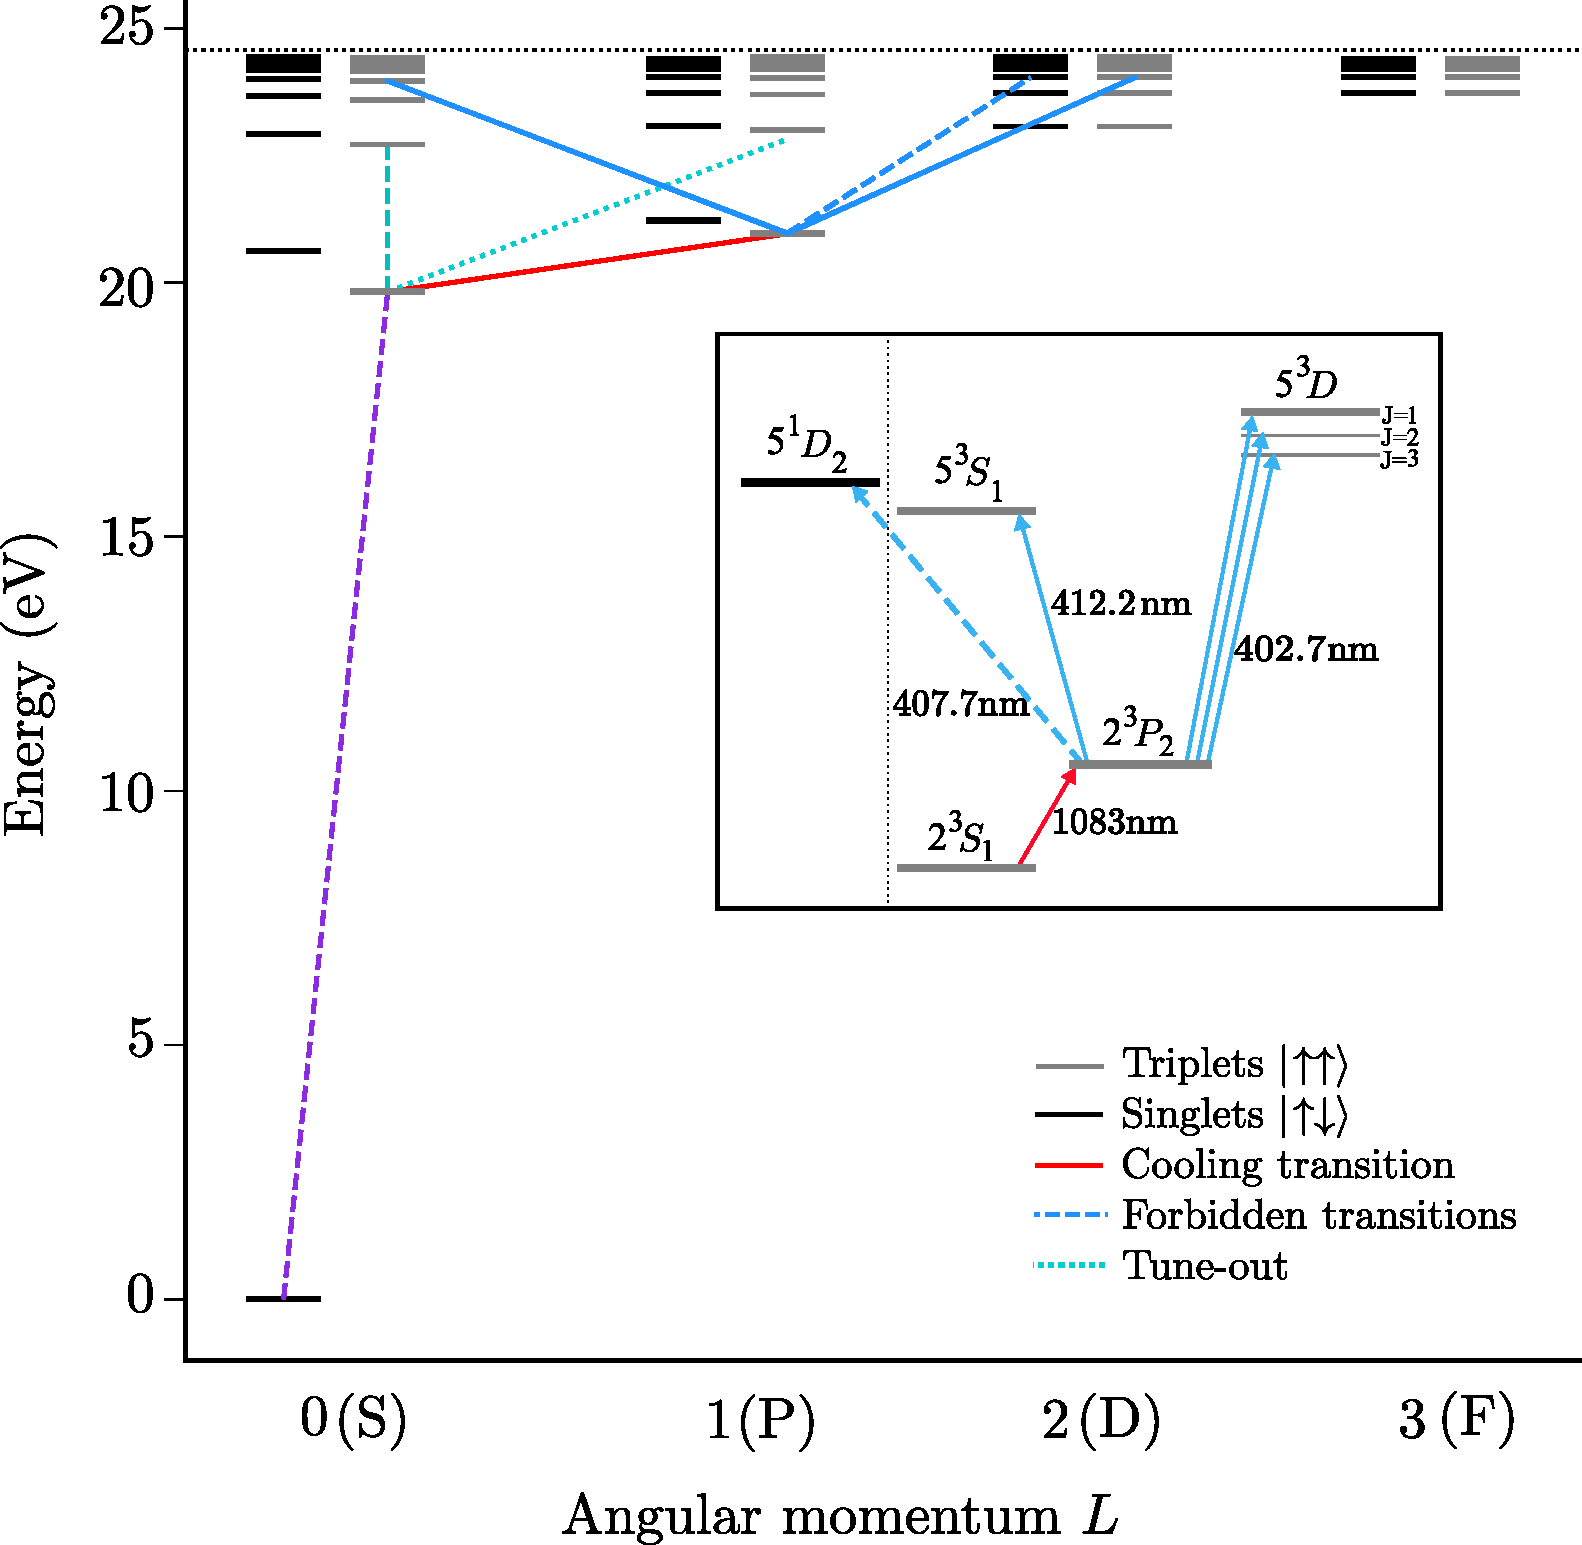
\includegraphics[width=\textwidth]{fig/introduction/full_lvl_diag.pdf}
		\caption{Energy levels of the singly-excited $^4$He atom, grouped by orbital angular momentum quantum number $L$. The $n=1$ manifold contains the unique $1^{1\!}S_0$ ground state - the Pauli exclusion principle precludes the existence of any $1^{3\!}S$ state. All singlet states (with total electron spin $S=0$) are marked with black lines, and the triplet states ($S=1$) in black. Levels up to $n=10$ and $L=3$ are shown along with notable optical transitions. The 1083.331nm cooling and trapping $2^{3\!}S_1\rightarrow2^{3\!}P_2$ transition is shown in solid red. The $63$nm transition between the ground and metastable excited $\MetastableState$ state is indicated in purple, and indicated as \emph{forbidden} by a dashed line. The transitions discussed in Chapter \ref{chap:transitions} and \cite{Ross20} are detailed in the inset (not to scale) , illustrating the fine structure splitting between states with different azimuthal quantum number $J$ which is too small to resolve at the scale of the main diagram. These were measured in the same campaign as the tune-out wavelength (dotted line, Chapter \ref{chap:tuneout} and Ref. \cite{Henson22}) and the forbidden $2^{3\!}S_1\rightarrow3^{3\!}S_1$ transition (reported in \cite{Thomas20}, not discussed in this thesis). The dotted line shows the 24.6 eV ionization threshold \cite{Drake07}.}
		\label{fig:full_level_diagram}
	\end{figure}

	The astute reader will notice the absence of presentation of an explicit form for the electron wavefunctions in the helium atom.
	Indeed,	helium is not analytically solvable because its eigenfunctions are not separable into a form $\Psi = \psi_1\otimes\psi_2$.
	A variational approach is required for tractable and accurate calculations, which was developed by Hylleraas \cite{Hylleraas1920,Hylleraas1929,Hylleraas1930}.
	In the intervening century, numerical methods for calculating the energy levels and transition rates in the helium atom have kept pace with precision experiments, and have incorporated the effects of relativity, nuclear recoil, and finite optical wavelength. A more detailed survey of recent progress is given in chapter \ref{chap:transitions}.

	

% Fine structure/sublevels; define 'manifold', 'term',' level', 'state' somewhere
	

	\subsection*{Magnetic fields and the Zeeman effect}

	The inclusion of spin introduces another important feature of atomic spectra, the Zeeman effect, whose discovery heralded a `watershed' moment of modern physics.
	The Zeeman effect refers to the phenomenon of spectral line splitting that occurs when an atom is immersed in a DC magnetic field\footnote{Oscillating magnetic fields have other effects on atoms, for example inducing magnetic dipole (or higher order) transitions involving spin-flips.}.
	The interaction energy of an atom in a magnetic field, 
	% \footnote{Along with  the discoveries of X-rays, radioactivity, and the observation that `cathode rays' had a mass-to-charge ratio equal to particles within atoms, now known as \emph{electrons}\cite{FootAtomic}}.
	
	% H spectrum provided observations to challenge class mech, then QM, then RQM, and indeed the current QED
	\begin{equation}
		H = -\text{\boldmath$\mu$}\cdot \textbf{B},
	\end{equation}
	has contributions from both orbital and spin angular momenta ($\textbf{L}$ and $\textbf{S}$, respectively) through the atom's magnetic moment,
	\begin{equation}
		\text{\boldmath$\mu$} = -\mu_B\textbf{L} - g_s\mu_B \textbf{S}.
	\end{equation}
	Working in the $\ket{LSJm_J}$ basis, where $J$ and $m_J$ are the total angular momentum and its z-projection, yields the energies $E_Z = g_J \mu_B B m_J$, where $\mu_B$ is the Bohr magneton..
	The atomic g-factor can be written as
	\begin{equation}
		g_J = \frac{3}{2} + \frac{S(S+1)-L(L+1)}{2J(J+1)},
	\end{equation}
	using the approximate value of the electron g-factor $g_s=2$.
	The eigenstates of the field-free atomic Hamiltonian will be $(2J+1)$-fold degenerate and specified by the $\ket{Lm_L S m_S}$ quantum numbers.
	Adding the magnetic field interaction breaks this degeneracy by introducing off-diagonal terms to the Hamiltonian when expressed in the $LS$ basis,  leading to the Zeeman splitting.
	The field-free and magnetic-interaction terms can be written in a common basis in terms of the Clebsch-Gordan coefficients and then diagonalized, as described in chapter \ref{chap:transitions}.
	The anomalous Zeeman effect arises in triplet states because the inter-level spacing depends on $m$ and $g_J$, which splits spectral lines as well as levels, whereas singlet states have $g_J=1$ and transitions between them do not fan out in the same fashion.
	
	% This distinction, whose explanation was an early victory for quantum mechanics, is illustrated in Figure \ref{fig:ZeemanLines}.
	

	% More than merely splitting lines, the Zeeman effect also induces a polarization-dependence  relative to the quantization axis.
	% The classical dipole envisions only circular polarization is visible along the quantization axis (z oscillation is not visible), but from transverse directions one can see the z oscillation and also the one-dimensional oscillations (eg along x when viewing the y axis) - so in a spatially varying mag field...
	% And we're nearly at the point of being able to project the Stokes vectors into the local field
	


	% RSP [10] ac stark shift -> dipole interaction, can include more levels for better calc [126] 
	% A Askkin acceleration and trapping of particles by radiation pressure, phys rev lett 24, 1970
	% RSP scattering happens [68] 
	% % Grimm, dipole traps
	
	For all the intricacy of atomic structure, life would be very dull indeed were it not for the interactions between them.
	Indeed, the material reality of the world depends, in a sense, less on the structure of its building blocks and more on how they fit together\footnote{This could be said to underpin the transferability of systems from a natural instantiation to analytic or simulated contexts, because there is truth in the \emph{structure} which is independent of the \emph{substrate} - this theme is elaborated in appendix \ref{chap:lattice}.}.
	The varied and central roles of interactions will be revisited in later chapters, traversing the spectrum from isolated, to weakly-interacting, to distinctly many-body systems.
	

\section{Interacting atoms}

	
	Here we briefly review elastic scattering, and then turn to important inelastic scattering processes present in our experiments.
	A detailed primer in atomic scattering physics can be found in the classic texts \cite{PitaevskiiStringari} and \cite{PethickSmith}, with more detail in the latter.
	An exhaustive review of low-temperature scattering studies up to the turn of the millenium can be found in \cite{Weiner99}.
	I focus here on two-body collisions, which are the dominant interactions in the low-density regime of ultracold helium.
	Low densities, which are necessary conditions to minimize the two-body loss processes characteristic to metastable helium, imply that low temperatures are required to achieve high phase space density and reach the degenerate regime.
	Two-body collisions are the crucial enabler for thermalization during the evaporative cooling employed to reach such low temperatures, so long as the relaxation times are shorter than the sample lifetime.

	Neglecting spin-orbit coupling and relativistic effects the two-body scattering problem reduces to the Schr\"{o}dinger equation in the centre-of-momentum frame,
	\begin{equation}
	\left(\frac{\hbar^2}{2m^*}\Delta + V(r) - E\right)\psi(r) = 0,
	\end{equation}
	where $\psi$ is the wavefunction capturing the relative motion of the two atoms	in terms of the separation $r=|\rvec_1-\rvec_2|$ between the particles and the reduced mass $m^*=m_1m_2/(m_1+m_2)$.
	In the asymptotic regime where $r$ is much larger than the scale of the interaction potential $V(r)$, the solution takes the form of a superposition of the initial plane wave and the scattered solution,
	\begin{equation}
	\psi(r) \propto e^{ikz} + f(\theta)\frac{e^{ikr}}{r},
	\end{equation}

	where $k=\sqrt{2m^*E/\hbar}$ is the plane wave-vector of the initial approach and $\theta$ is the angle of scattering from the direction of incidence.
	A general solution can found by expanding $f(\theta)$ into a convenient basis of \emph{partial waves} (spherical harmonics) which are labeled $s,p,d,f,..$ in order of increasing angular momentum.
	In the low-energy limit, $f(\theta)$ is independent of angle and only the spherically symmetric s-wave term contributes, and the limit $f(\theta)\rightarrow-a$ is accordingly called the s-wave scattering length.
	In the millikelvin regime the scattering physics is determined by just a few partial waves \cite{McNamara07}, and in the ultracold (microkelvin or colder) regime only the s-wave scattering channel is significant.
	The total cross section, which is the total probability that a near collision results in particle scattering, approaches $\sigma=8\pi a^2$ for polarized bosons\footnote{For fermion pairs with odd total spin, the cross section tends to zero because of the Pauli exclusion principle, and thus the s-wave scattering length vanishes.} \cite{PitaevskiiStringari,Przybytek05}.
	

	The s-wave scattering length is also an important determinant of the energetics of degenerate matter such as BEC.
	Because BECs are dominated by long-wavelength behaviour, a theoretical treatment can be considerably simplified by considering only the \emph{effective interactions}.
	By formulating the scattering problem in momentum space, the effective interaction strength for low-energy scattering  $g=4\pi \hbar^2 a/m$, also referred to as the pseudopotential, can be found by integrating out the high-frequency modes (also known as the Born approximation).
	This necessarily washes out extremely short-range correlations but makes fairly accurate calculations much more tractable by reducing the size of the basis set used in a calculation.

	In molecular collisions the scattering process will obviously depend on the relative orientation of the molecules.
	In collisions between single atoms, though, there is a more subtle orientation-dependence which arises from the total spin of the two-particle system.
	The three possible configurations between pairs of \mhe~atoms correspond to the singlet $^1\Sigma_g^+$, triplet $^3\Sigma_u^+$, and quintet $^5\Sigma_g^+$ Born-Oppenheimer molecular potentials\footnote{The subscript \emph{g} and \emph{u} are short for \emph{gerade} and \emph{ungerade} (German for even and odd) label the reflection symmetry of the two-body wavefunction.} with total spin 0, 1, and 2 .
	When the atoms are spin-polarized, as \mhe~atoms are when confined in magnetic traps, then the only scattering that occurs is in the quintet channel.
	In low-energy scattering contexts dominated by s-wave scattering, odd partial waves do not contribute to the interaction potential and hence the triplet $^3\Sigma_u^+$ potential is dominated by the quintet $^5\Sigma_g^+$ term for all interactions with nonzero total spin \cite{Leo01}. 
	As such the inter-species scattering lengths $a_{1,1}$, $a_{-1,-1}$, $a_{0,1}$, and $a_{0,-1}$ are all equal \cite{Leo01,Vassen16}.
	The most accurate determination of the s-wave scattering length in these configurations is 7.512 nm \cite{Moal06}, in agreement with calculations performed the year before the measurements \cite{Przybytek05}.
	When the total spin is zero, the singlet potential contributes and so $a_{1,-1}\approx8.8$ nm and $a_{0,0}\approx3.8$ nm \cite{Leo01,Vassen16}.
	In general this thesis will be concerned with interactions between spin-polarized helium atoms and hence will use the abbreviation $a\equiv a_{1,1}$ unless specified otherwise.
	

	A powerful tool available in some cold atom experiments are Feshbach resonances.
	A detailed description is found in \cite{Chin10}, but from an operational standpoint they allow control of the scattering length as $a = \tilde{a}(1-\Delta/(B-B_0))$, where B is the strength of an ambient magnetic field, $B_0$ is the resonance value of the field, $\tilde{a}$ is the value when the field is far from a resonance and $\Delta$ sets the resonance width.
	The scattering length can thus be tuned in size and even in sign.
	However, the stability of a BEC with arbitrary population requires a positive s-wave scattering length.
	Attractive interactions leading to instability and collapse of a condensate with number above a critical value $N_\textrm{cr}\sim\mathcal{O}(a_{ho}/|a|)$, where $a_{ho} = \sqrt{\hbar/m\omega}$ is the length scale of the ground state of the harmonic trap housing the atoms \footnote{In some negative-temperature states created in an optical lattice, a BEC can be stable with attractive interactions \cite{Braun13}.} \cite{PitaevskiiStringari}.
	Switching from stable to unstable configurations permits one to examine condensate collapse (as in the spectacular Bosenova experiments \cite{Cornish00}) and also to explore the BEC-BCS crossover \cite{Bourdel04}.
	The spinless nucleus of $^4$He prohibits coupling of bound states within an $m_J$ manifold from crossing an open-channel threshold, precluding this pathway to a Feshbach resonance \cite{Goosen10}.
	Nonetheless, Feshbach resonances induced by spin-spin interactions between helium atoms have been predicted \cite{Venturi99, Goosen10}, but have not observed to date \cite{Borbely12}.
	In a recent work \cite{Hirsch21}, the authors (including members of the ANU He* lab) describe calculations with a newer method predicting, unfortunately, the absence of Feshbach resonances between $^4$He-$^4$He collisions.
	
	Inelastic scattering processes are those which exchange energy between the internal and motional states of either atom.
	They can be represented as a complex scattering potential \cite{Leo01} which permits losses from on-shell scattering channels.
	An important inelastic process characteristic of metastable noble gases is \emph{Penning ionization} \cite{VassenReview}.
	 This can occur through the decay channels
	\begin{equation}
		\textrm{He}^*+\textrm{He}^*\rightarrow 
		\begin{cases}
			\textrm{He}+ \textrm{He}^+ + e^-&\textrm{(PI)}\\
			\textrm{He}_{2}^{+} + e^-&\textrm{(AI)}
		\end{cases}
	\end{equation}
	wherein the first channel is formally called Penning ionization and the second is  Auto-ionization and the rate of the latter is generally very small in comparison to the former \cite{Muller91}.
	Indeed, the energy of the metastable state is sufficient to ionize any neutral atom (except helium or neon) from its ground state, and underpins the single-atom sensitivity of our solid state detector (described in section \ref{sec:DLD}).
	Aside from attracting intensive study in its own right \cite{Partridge10,Stas06,McNamara07}, this explosive potential was a significant hurdle for researchers attempting to achive Bose-Einstein condensation with helium.
	The density achieved in early magneto-optical traps (MOTs) was limited to some hundredfold less than the alkali-metal MOTs of the day \cite{Bardou92,Kumukura92,Mastwijk98}.
	Helium MOT densities were limited by losses through two-body collisions involving atoms in the $\metastable$ and those excited to the $2\triplet P_2$ state by the trapping beams, as opposed to rescattering pressure as in the case of alkali metals.
	Indeed, while the Penning loss rate constant\footnote{The rate constant $\beta_{i,j}$ for losses via collisions between atoms in states $i$ and $j$ yields an absolute loss rate per volume per time through the product with the respective densities, $\Gamma_{i,j} = \beta_{i,j}n_i n_j$ cm$^{-3}$s$^{-1}$.} between pairs of $\metastable$ atoms is of order $2\times10^{-9}$ cm$^3$/s, the loss rate for $\metastable-2\triplet P_2$  collisions is around $10^{-7}$ cm$^3$/s.
	Thus early MOTs had loss rates which were a population-weighted average of these rates, around $7\times10^{-8}$ cm$^3$/s \cite{Weiner99}.
	Such light-assisted losses  limited the population achievable in MOTs until larger beams and detunings were used \cite{Tol99}.
	The Penning ionization rate is some 20-fold lower at large detunings compared to near-resonant light \cite{Mastwijk98}, reducing this loss rate to the order of $5\times10^{-9}$ cm$^3$/s at large detunings.
	Fortunately, the inelastic scattering cross-sections depend on the molecular potentials in such a way that condensation becomes attainable: When all the atoms are polarized in the either of the $m_J=\pm1$ states, the incoming state has a total spin of 2, whereas the reaction products have a total spin of 1, and so this process is forbidden.
	In reality, it does occur through a weak virtual spin-dipole transition \cite{Shlyapnikov94}, but slowly enough that spin-polarized \mhe~exhibits a $10^4$-fold reduction in the Penning ionization rate.
	At field strengths above 50 G, however, the suppression weakens \cite{Shlyapnikov94,Borbely12}.
	Other noble gases also exhibit highly energetic metastable states, but the lifetime and suppression of Penning ionization decreases with increasing mass \cite{Orzel99, Spoden05}.
	Thus helium may be the only noble gas ever to cooled to degeneracy.
	
	% F bardou, O emile, J M courty, C I Westbrook, A Aspect, magneto-optical trapping of metastable ehlium: Collisions in the presence of resonant light, Europhysics letters 20, Dec 1992
	% M Kumakura N Morita, visible observation of metastable helium atoms confined in an invisible/visible resonance trap, japanese journal of applied physics 31, march 1992
	% H C Mastwijk, J W thomsen, P van der straten, A niehaus, optical collisions of cold, metastable helium atoms, physical review letters 80, june 1998

	% \cite{Shlyapnikov94} predicts 1e5x reduction in PI in spin-pol samples; relaxation-induced penning; virtual spin-dipole transitions (induced by spin-dipole interaction) to the zero spin state of the quasimolecule can lift the spin-conservation rule and lead to regular penning ionization	Direc dipole-exchange ionization is also a possibility but dominated by spin-relazation (relaxation-induced penning; virtual spin-dipole transitions to the zero spin state of the quasimolecule can life the spin-conservation rule and lead to regular penning ionization)
	
	
\section{Bose-Einstein condensation}
\label{sec:BEC_theory}

		% M H ANderson, J R Ensher, M R Mathews, C E Wieman, and E A cornell, observation of bose-einstein condensation in a dilute atomic vapor, Science 269, 198-201, July 1995
		% K B Davis, M O Mewes, M R Andrews, N J van Druten, D S Durfee, D M Kurn, W Ketterle, Bose-Einstein condensation in a gas of sodium atoms - Physical Review Letters 75, 3969-3973, Nov 1995
		% C C Bradley, C A Sackett, J J Tollett,  G Hulet, evidence of Bose-Einstein condesnation in an atomic gas with attractive interactions, phyiscal review letters 75, 1687-1690, aug 1995
		% W D Phillips, H Metcalf, Laser deceleration of an atomic beam, Phys Rev Lett 48, 1982
		% Chu et al, three-dimensional viscous confinement and cooling of atoms by resonance radiation pressure, phys rev lett 55, 1985
		% Ch et al, experimental observation of optically trapped atoms, phys rev lett 57, 1986
		% Raab et al, trapping of neutral sodium atoms with radiation pressure, phys rev lett 59, 1987
		% P D Lett et al, observation of atoms laser cooled below the Doppler limit, phys rev lett 61, 1988

	% \subsection{What is a BEC?}
	% Things I might like to put in later: Partition function Z = Tr(\exp(\beta H)), expectation values Tr(O rho)/Z, 

	The fifth state of matter\footnote{The familiar first phases, solid, liquid, and gas, are vanishingly rare in cosmological terms.
	The fourth, plasma, is the state of at leats 99\% of the ordinary matter in the universe \cite{Plasmastuff}.
	Helium comprises about 23\%, most of which being primordial baryons formed during the recombination epoch.}  has a long and storied history\cite{Mukundanote}.
	Interest in BEC was amplified back in the middle of the 20th century when Fritz London proposed that Bose-Einstein condensation was connected to the superfluid phenomenon in liquid helium.
	Nikolay Nikolayevich Bogolyubov formalized this connection and so, historically speaking, helium was the element which hosted the earliest experimental realization of Bose-Einstein condensation, albeit with a very small condensed fraction\footnote{Nikolay was a darling of Russian theoretical physics, receiving his PhD-equivalent qualification at 19 and made important contributions to quantum field theory. In his famous paper on the problem of interacting bosons, his name is transliterated as \emph{Bogolubov}. \emph{Bogolyubov} and \emph{Bogoliubov} are also common transliterations.}.
	While liquid helium is a rare thing in cosmological terms, BEC may have existed already for millions of years in the superdense quark matter of neutron stars \cite{Haskell18, Martin16,Baym69,Page11}, wresting the claim of cosmic novelty from human hands. 
	Nonetheless, the essentially pure atomic condensates and the emerging study of molecular condensates in laboratory settings are among the most extreme conditions in the universe, and are not believed to occur naturally elsewhere.
	Following the oft-cited seven decades between the initial theoretical descriptions and the experimental realization of atomic Bose-Einstein condensates (BEC) \cite{Davis95,Bradley95,Anderson95}, the field has become quite industrious at the eve of its centenary.
	As pithily put by a review only five years after the Nobel-winning experiments, `Any attempt to review recent progress is out of date as soon as it is published' \cite{Courteille01}.
	This is no less true today, as the number of ultracold quantum gas experiments worldwide\footnote{See \url{everycoldatom.com}} now number nearly 200 and numerous companies have been founded on the promise of selling better sensors and computers using technologies based on BEC physics.
	There are numerous treatments of the theory of Bose-Einstein condensation, for example the classic textbooks \cite{PitaevskiiStringari,PethickSmith} and review articles \cite{Dalfovo99, Yukalov11_basics,Courteille01}.
	The essential background for discussion here draws on these standard sources unless otherwise cited.
	% anquez16 also cites Bogoliubov theory as being used in analysis of quantum phase transitions in spinor condensates


	% There's something to be said here; there is a distinction between the ground state, which is global, and the single-particle states...
	As for what a BEC \emph{is}, there are several workable operational definitions, but a precise and lab-relevant definition is surprisingly elusive.
	The canonical description of Bose-Einstein condensation is the condition where the de Broglie wavelength associated with thermal kinetic energy
	\begin{equation}
		\lambda_T = \frac{h}{\sqrt{2\pi m k_B T}}
	\end{equation}
	is comparable to the interparticle spacing, coinciding with a macroscopic occupation of the single-particle ground state as the de Broglie waves of many bosons constructively interfere.
	This condition can also be restated as the point when the phase space density
	\begin{equation}
		\aleph = n \lambda_T^3
	\end{equation}
	exceeds the critical value of $\zeta(3)\approx2.612$. 
	This is generally introduced of as the point where the volume over which the atoms are `delocalized'  exceeds the average volume per particle, and so the spin-statistics of the particles dictate the deviation from the statistics of an ideal gas.
	Although it is commonly said that at this point the `wavefunctions overlap', the wavefunctions of the individual particles in a trapped gas overlap wherever the wavefunction is supported - that is, throughout the trap.
	Furthermore, the de Broglie wavelength pertains to the wavelength associated with the plane-wave motion of a free particle rather than the spatial scale of the `wavepacket' of a particle, and as given above is defined as the wavelength corresponding to the \emph{average} particle velocity, rather than fully characterizing the ensemble. 
	Thus even above the critical temperature there are many states with long wavelengths who will be populated, and so the `delocalization' picture is not so sharp.
	A more precise criterion is to compute, in the framework of the grand canonical ensemble, the number of particles in the ground state. For a Bose gas this yields
	\begin{equation}
		N_0 = \frac{1}{\exp((E_0-\mu)/k_B T)-1},
	\end{equation}
	where $E_0$ is the ground state energy of the single-particle Hamiltonian and $\mu$ is the chemical potential of an adjoining reservoir. 
	One can then show that, below the critical temperature $T_c$, the ground-state population diverges, corresponding to Bose-Einstein condensation.
	However, in laboratory realizations of BEC, there is no reservoir attached to the system under study, but rather an isolated gas at some finite entropy which contains both the thermal and condensed fractions (if the latter is present). 
	
	Moreover, in the presence of interactions, this criterion faces another issue: the stationary states of an interacting gas of $N$ atoms cannot be written as a product $\ket{\Psi} = \ket{\psi_i}^{\otimes N}$ of single-particle eigenstates $\ket{\psi_i}$.
	That is, while measurements are confined to observables of single particles, the single-particle states are not eigenstates and so it is not sensible to talk of their `macroscopic occupation'.
	The Penrose-Onsager criterion \cite{Penrose56} provides an alternative in terms of the density matrix $\rho$ for the isolated composite system comprised of all the gas particles.
	The single-particle density matrix is then the expected value of the one-body field operator
	\begin{equation}
		\rho^{(1)} = \Tr\left(\rho\hat{\Psi}^\dagger\hat{\Psi}\right),
	\end{equation}
	whose eigenvalues $p_{l}^{1}$ give the occupation probability of the $l^{\rm th}$ eigenvector of $\rho^{(1)}$.
	The eigenvectors themselves are the single-particle modes (which may be, in general, some superposition of the non-interacting eigenstates).
	If any eigenvalue $p_{l}^{i}$ is proportional to $N$ in the limit $N\rightarrow\infty$, then the system is said to have undergone Bose-Einstein condensation (or, simply, \emph{condensed}) into the $l^\textrm{th}$ mode.
	Of course, real systems are subject to atom losses and heating, violating the assumptions of equilibrium underpinning both the approaches above.
	
	This is all to illustrate the point that the real world is full of intricacies and the `intuitive' pictures of BEC, despite being useful pedagogical tools, can skirt around some important physical features.
	Ultimately though, this is a thesis concerned with experiments, and we shall say little more than remarking on the compelling agreement between abstract and actual condensates irrespective of the preceding issues.
	Indeed, the Penrose-Onsager criterion has been shown to be a good characterization of a non-Hermitian polariton condensate \cite{Manni12} in that off-diagonal long range order (i.e. phase coherence) emerges along with the growh of a single eigenvalue of the one-body density matrix.
	As the saying goes, if it interferes like a condensate \cite{Andrews97} , undergoes number fluctuations like a condensate \cite{Kristensen19},  has HBT correlations like a condensate \cite{Schellekens05,Jeltes07}, Kibble-Zureks like a condensate \cite{Anquez16}, and quacks like a condensate \cite{Duck01}, then it probably \emph{is} a condensate.

	While most atomic condensates, and all of those in this thesis, are trapped in non-uniform potentials, many important features of condensates are easier to state for homogeneous systems.
	One can usually extend calculations to harmonically trapped systems by a local density approximation, wherein one performs a density-weighted average across a condensate, considering each volume element as a homogenous condensate in its own right.
	Thus, for the most part the following discussion will focus on homogeneous systems for simplicity's sake.
	I present some particular results in the case of a harmonically trapped gas at the end of this section.

	% \todo{ODLRO links}
		% https://physics.stackexchange.com/questions/79846/what-is-off-diagonal-long-range-order-in-superfluid
		% https://arxiv.org/abs/1804.04084

	% distinction worth making; the ground state is a global property of the configuration.
	% Interactions mean it is not the same as the product of single-particle ground states: I mean, it *is* actually in this case, I think, but the ground states are not solutions of a free hamiltonian (I guess they are in the bogo pictures though??)


	% Potential for historical note about liquid helium
	
	%  Potential resolution; Mastsubara (1955) A new approach to quantum-statistical mechanics, Progress of Theoretical Physics vol 14, no 4
	% Many characteristic features predicted for Bose-Einstein condensates have been observed in ultracold trapped gases.
	
	% Something something grand-canonical ensemble; role of chemical potential; tracing out reservoir
	% We have the other formlation, \rho = \exp(\beta \hat{H});
	\subsection*{Bogoliubov theory}
	The fundamental theoretical object of interest is the Hamiltonian of a bosonic quantum field with two-body interactions $\hat{H} = \hat{K} + \hat{I}$, with kinetic part
	%mark
	\begin{equation}
		\hat{K} = \int\left(\frac{\hbar^2}{2m}\nabla\hat{\Psi}^\dagger(\textbf{r})\nabla\hat{\Psi}(\textbf{r})\right)d\textbf{r}
		\label{eqn:ham1}
	\end{equation}
	and the interaction term
	\begin{equation}
		\hat{I} = \frac{1}{2}\int\left(\hat{\Psi}^\dagger(\textbf{r}')\hat{\Psi}^\dagger(\textbf{r})V(\textbf{r}'-\textbf{r}) \hat{\Psi}(\textbf{r}')\hat{\Psi}(\textbf{r})\right)d\textbf{r}'d\textbf{r}
		\label{eqn:ham2}
	\end{equation}
	where $\Psi(r)$ are the field operators subject to the bosonic commutation relations
	\begin{align}
		[\Psi(r),\Psi^\dagger(r')] &= \delta(r-r')\\
		 [\Psi^\dagger(r),\Psi^\dagger(r')]&=[\Psi(r),\Psi(r)]=0.
	\end{align}	
	We can then write the field operator in the suggestive form	
	\begin{align}
		\hat{\Psi} &= \psi_0 \hat{a}_0 + \sum_{i\neq0}\psi_i \hat{a}_i
	\end{align}
	in terms of an orthonormal basis of single-particle modes $\psi_i$ and corresponding field operators $\hat{a}_i$.
	In doing so we distinguish $\pvec=0$ as the condensed mode, and say that condensation occurs when $N_0=\langle\hat{a}^\dagger_0\hat{a}_0\rangle =\mathcal{O}(N)$.
	The observation that the condensed mode has a population of order $N$ means that in the thermodynamic limit ($N\rightarrow\infty,~V\rightarrow\infty$), one particle here or there will not really make a measurable difference.
	% More quantitatively, one could say $\hat{a}_0\psi_0 = 
	This argument can be expressed quantitatively as the Bogoliubov approximation wherein the annihilation and creation operators for the condensed mode are replaced with complex numbers as per
	\begin{equation}
		\hat{a}_0 = \sqrt{N_0}e^{i\alpha}, \hat{a}_0^\dagger= \sqrt{N_0}e^{-i\alpha}, 
	\end{equation}
	which permits the condensate wavefunction to take the form
	\begin{align}
		\hat{\Psi} &= \sqrt{N_0}e^{i\alpha} \psi_0 + \delta\hat{\Psi}\\
					&= \Psi_0 + \delta\hat{\Psi}
	\end{align}


	% Where  $\sqrt{N_0}e^{i\alpha}$ is the \emph{order parameter} which gives the amplitude of the condensate wavefunction and $\psi_0$ is some self-consitent defn of the condensed mode, however one gels the atom-density-matrix defn with the bosonic field...
	

	% usuall The eigenfunctions of the non-interacting(?) case can be used to express the field operator $\Psi(r) = \sum_i \phi(i) \hat{a}_i$ in terms of the creation operator, which obeys similar commutation relations.
	% This then leads to a similar separation of the field operator into the condensed and noncondensed part,
	% % $$
	% % \Psi(r) = \phi_0\hat{a}_0 + \sum_{i\neq0}\phi_r(r)\hat{a}_i,
	% % $$
	% % Does bogo assume $[\hat{a}_o,\hat{a}^{\dagger}_0] = 0$? 
	% % form is then $\Psi(r) = \Psi_0(r) + \delta\Psi(r)$ where the first term on RHS is the complex fn $\sqrt{N_0}\phi_0$ and the last term is a sum over other modes.
	
	% %%See also; assuming \Psi = \phi + \hat{\psi} with \int|phi|^2 >> \langle\psi^\dagger\psi\rangle permits discarding third-and-higher order terms in the full bosonic field hamiltonian, leading to GPE...
	% how relates to Born approx?
	The first term is the condensate wavefunction (the \emph{mean-field} term), and the second corresponds to the population of non-condensed modes thanks to the effect of interactions, which are captured by the quasiparticle picture sketched in the next section.	The emergence of a condensate has many of the hallmarks of a classical phase transition: kinetic effects are necessary to redistribute energy and reach steady-state; a unique critical temperature $T_c$ exists; below $T_c$ an \emph{order parameter} takes on a nonzero value; and condensation is equivalent to the spontaneous breaking of a U(1) gauge symmetry \cite{Yukalov11_symmetry}.
	Above the critical temperature, $|\Psi_0|=0$, and in general it exhibits a discontinuous derivative at the critical temperature.
	Hence, in the Landau-Ginzburg framework, condensation is a second-order phase transition\footnote{In the Ehrenfest picture one is instead concerned with the number of times one must differentiate some state function (e.g.
	specific heat, compressibility, pressure, free energy) before finding a discontinuity at the critical point.
	In this picture, the transition is first-order as one has continuous state functions with discontinuous derivatives.}.
	The other hallmark of Landau-Ginzburg phase transitions is the spontaneous breaking of symmetry as one crosses from the disordered to the ordered phase (as when a solid breaks the translational symmetry of the fluid phase).
	Condensates do exhibit such symmetry breaking: The Hamiltonian has a $U(1)$ gauge symmetry, but the ground state of a condensate spontaneously chooses a fixed but unpredictable phase $\alpha$.
	By interfering two independently prepared condensates, one observes interference fringes \cite{Andrews97}, and indeed, the fringe locations will change with each realization and measurement.
	More directly, one can interfere light leakage from a reservoir-coupled photon condensate against a reference beam, and observe that phase jumps occur in the output when the condensate field drops to zero.
	That is, the re-emergence of the condensate is heralded by the selection of a new, specific, phase, apparently uncorrelated with the phase that existed before it \cite{Schmitt16}.
	
	
	Symmetry breaking is a subtle point discussed infrequently in standard textbooks.
	It happens that one can substitute complex numbers for the field operators,  even when $\langle N_0\rangle \rightarrow 0$ and still obtain correct results \cite{Ginibre67}.
	That is, condensation is not necessary for the Bogoliubov approximation to be valid.
	However, it \emph{is} the case that the onset of condensation coincides with the ground state breaking\footnote{This is sometimes called `breaking the gauge symmetry'.
	This is a misnomer, as a gauge symmetry is a property of the theory, not a state, and all consistent theories must be gauge symmetric throughout.
	These subtleties are discussed at length in lucid terms in \cite{Poniatowski19}.} the $U(1)$ symmetry \cite{Suto05}.
	
	% That this coincides with the validity of the `coherent state' approximation is quite profound: Like the transition from the quantized electromagnetic field to the Maxwell equations, BEC has the flavour of a classical field but one which is consitued by matter which has dispersed in some delocalized state.
	% The interactions between atoms present a marked departure from the physics of the electric field, however, and yet the system remains in the grasp of human theorists thanks to the Bogoliubov approximation, which I introduce here and examine experimentally in chapter \ref{chap:QD}.
	% %  First-order phase transition as the chemical potential has a discontinuous derivative \cite{Ykalovreview}, cf ehrenfest critioerion of discontinuous derivative of a state function; the ginzburg-landau classification is in terms of the order parameters; BEC is a second-order transition as the order parameter is continuous with a discontinuous derivative.
	% % Penrose and Onsager generalized the definition of condensation to include interacting particles and non-uniform systems.
	%  In fact, the Bogoliubov picture of superfluidity actually refers to a condensation of non-interacting collective bosonic modes, rather than the condensation of the constituent atoms.
	% The definitions coincide fairly well.../
	% % NB most BEC theory most simply stated for homogeneous systems, so will consider these initially, and return to a few remarks about harmonically trapped gases at the end of the section.


	% Actually in the following, one starts from the full second quantized hamiltonian and assumes smooth density in the born approx to get to the  GPE.
	% The variational approach is just an alternative and need not be included.
	
	
	
	\subsection*{Harmonically trapped condensates}

	Turning back toward harmonic gases, we can begin from the full Hamiltonian (Eqns.
	(\ref{eqn:ham1},\ref{eqn:ham2}) and produce an effective Schr\"{o}dinger equation.
	By assuming slow variations in the density, integrating out short-wavelength modes as in the Born approximation, one can derive the Gross-Pitaevskii equation (GPE),
	\begin{equation}
		i\hbar\frac{\partial \Psi_0(r,t)}{\partial t} = \left(-\frac{\hbar^2\nabla^2}{2m} + V(r,t) + g|\Psi_0(r,t)|^2\right)\Psi_0(r,t).
		\label{eqn:GPE}
	\end{equation}
	which is valid for arbitary interactions dominated by the s-wave scattering length.
	 If one further assumes that the condensate density varies on scales larger than the healing length $\xi = \hbar/\sqrt{2mgn}$, one can make the Thomas-Fermi approximation and ignore the kinetic term in the GPE, whereby the condensate density profile can be written as

	
	\begin{equation}
		n(\textbf{r}) = \frac{\mu-V(\textbf{r})}{g},
	\end{equation}
	where $\mu$ is the chemical potential.
	The chemical potential for the harmonically trapped condensate also fixes the average energy per particle as
	\begin{equation}
		\mu = \frac{7}{5}\frac{E}{N} = \frac{\hbar\bar{\omega}}{2}\left(\frac{15 N a}{a_{ho}}\right)^{2/5} ,
	\end{equation}
	recalling $a_{ho} = \sqrt{\hbar/m\bar{\omega}}$ is the length scale of the ground state of the harmonic oscillator, with $\bar{\omega}$ being the geometric mean of the $x$, $y$, and $z$ trapping frequencies.
	For a Bose gas confined in a harmonic potential of the form
	\begin{equation}
		V = \frac{1}{2} m \omega_x^2 x^2 + \frac{1}{2} m \omega_y^2 y^2 + \frac{1}{2} m \omega_z^2 z^2,
	\end{equation}
	the condition $\mu-V(\textbf{r})=0$ determines the boundary of the condensate, giving the Thomas-Fermi radii $R_i = \sqrt{2\mu/m \omega_i^2}$, where $i\in\{x,y,z\}$.
	This produces the famous inverted-parabola density profile with a peak density of
	\begin{equation}
		n_0 = \frac{1}{8 \pi}\left( (15N_0)^2 \left(\frac{m \bar{\omega}}{\sqrt{a \hbar}}\right)^{6}\right)^{1/5}.
		\label{eqn:n0}
	\end{equation}
	The Thomas-Fermi approximation is valid when $N a/a_{ho}\gg1$. 
	This is when the mean-field energy significantly outweighs the kinetic term.
	The phase space density for condensation is achieved at the (ideal) critical temperature 
	\begin{align}
		T_c^{0} &= \frac{\hbar \bar{\omega}}{k_B}\left(\frac{N}{\zeta(3)}\right)^{1/3}\\
				&\approx0.94\frac{\hbar \bar{\omega} N^{1/3}}{k_B}.
	\end{align}
	where $\bar{\omega}=(\omega_x\omega_y\omega_z)^{1/3}$ is the geometric mean of the trapping frequencies, and the condensed fraction below the critical temperature is 
	\begin{equation}
		\frac{N_0}{N} = 1 - \left(\frac{T}{T_c^{0}}\right)^3.
	\end{equation}
	The rest of the population, occupying excited single-particle states, is called the thermal fraction.
	The population $N_T$ of the thermal fraction saturates as $\frac{N_T}{N} = \left(\frac{k_B T}{\hbar \bar{\omega}}\right)^3$ in a non-interacting Bose gas, wherein any atoms added to the gas fall into the condensate mode, regardless of the density of the gas.
	Real gases generally don't show such a feature, and this bifurcation is corrected by including the effect of interactions on the thermodynamics of the Bose gas.	 
	Interactions between particles reduce the critical temperature in a harmonic trap, which can be understood in terms of repulsive interactions reducing the density at a given temperature and thus requiring a lower temperature to achieve a give $\aleph$.
	The resulting shift in the critical temperature can be supplemented with a correction for the finite population of the condensate and written as
	\begin{equation}
		\frac{\delta T_c}{T_c^{0}} = -1.3 \frac{a}{a_{ho}} N^{1/6} -0.73\frac{ \langle\omega\rangle}{\omega_{ho} N^{1/3}}
	\end{equation}
	where the latter term, the correction for finite atom number, includes the arithmetic mean trapping frequency $\langle\omega\rangle$ and vanishes in the thermodynamic limit $(N\rightarrow\infty,~V\rightarrow\infty,~N/V$ finite).
	These deviations from ideal behaviour have been observed in experiments \cite{Tammuz11,Smith11}.

	% For an ideal gas, this is the expected fraction of the population in the ground state of the trap.
	As for the practical production of condensates, much quality literature has been written on the theory and techniques of atomic cooling employed to reach degeneracy.
	These days, such techniques are standard across hundreds of laboratories and so space will not be spared for their general consideration here.
	The curious reader is directed to \cite{MakingProbingUnderstanding,Courteille01,MetVdS, TychkovThesis} for detailed discussions.
	Rather, in the next chapter I discuss the specifications of the apparatus I used in the course of this research. 
	
\subsection{Cooling techniques}
	\label{sec:doppler_basics}
	In brief, both BEC machines discussed in this thesis exist to achieve magnetic trapping of metastable helium in ultra-high vacuum (UHV) conditions, and from there apply further operations as required by the science at hand.
	Magnetic trapping is required because the limits of optical cooling are too hot to achieve degeneracy with the densities realizable with optically trapped helium.
	However, optical cooling is a necessary first stage of cooling to reach the cold (millikelvin) regime before evaporatively cooling to the ultracold (microkelvin) regime en route to degeneracy in the nanokelvin regime.
	Doppler cooling is the most-used optical cooling technique in this thesis for two main reasons.
	First, helium's spinless nucleus means it has no hyperfine structure and precludes some other forms of sub-Doppler cooling.
	Second, Doppler cooling is sufficient to reach phase space densities high enough to seed evaporative cooling sequences which achieve condensation. 
	
	% H F Hess, Evaporative cooling of magnetically trapped and compressed spin-oolarized hydrogen, Physical Review B 34, 3476-3479, Sept 1986
	% W Ketterle and N J van Druten, Evaporative cooling of traped atoms, advanes in atomic molecular and optical physics 37, 181-236, 1996
	% O J Luiten, M W reynolds, J T M Walraven, Kinetic theory of the evaporative cooling of a trappe dgas, Physical Reveiw A 53, 381-389 Jan 1996
	Doppler cooling effectively produces a velocity-dependent force by exploiting both radiative pressure and the Doppler effect, which I illustrate here with reference to a two-level atom with resonant frequency $\omega_0$.
	An atom moving with velocity $\vec{v}$ with respect to the source of a laser (approximated as a plane wave with wavevector $\vec{k} = \omega/c$ in the reference frame of the laser emitter) will see a radiation field with a Doppler-shifted frequency $\omega' = (1 - \vec{k}\cdot \vec{v}/c)\omega$.
	If the laser is detuned from the transition one has the resonance condition $\vec{k} \cdot \vec{v}/c = (1 - \omega_0/\omega)$, hence if the detuning $\Delta = \omega-\omega_0$ is negative (i.e. the laser is \emph{red} of the resonance) then the light is Doppler-shifted into resonance in the atomic frame for some $\vec{k} \cdot \vec{v}<0$, i.e. when the atom is moving toward the source of the laser. 
	When the atom absorbs a photon and is excited to the upper state of the transition it acquires the photon recoil momentum $\vec{p} = \hbar \vec{k}$.
	If the laser is red-detuned then this impulse opposes the atomic motion along the $\vec{k}$ direction and slows the atom down.
	The atom eventually decays to the ground state on a timescale $\tau = 1/\Gamma$ where $\Gamma$ is the excited-state linewidth.
	The emission events (at a rate $\Gamma$) are isotropic and so the integrated momentum imparted from the many emission recoils is zero.
	The atom is then excited again at a rate $\Gamma_{sc}$ (the real part of Eqn. \ref{eqn:lorentzian}), which can be written 
	\begin{equation}
		\Gamma_{sc} = \frac{s}{2 }\frac{\Gamma}{1 + s + (2\delta/\Gamma)^2}
	\end{equation}	
	in terms of the (atom-frame) detuning $\delta$ and $s=I/I_\textrm{sat}$, where the saturation intensity $I_\textrm{sat} = \pi h c \Gamma/(3\lambda^3)$ is $0.167$ mW/mm$^2$ for the cooling transition in \mhe~\cite{BaldwinReview}.
	The cycling absorption-emission events culminate in an effective force $\vec{F} \approx \Gamma_\textrm{sc}\hbar\vec{k}$ (when $\Gamma_\textrm{sc}>\Gamma$) called the \emph{radiative force}. 
	The scattering rate $\Gamma_\textrm{sc}$ depends on the detuning, hence the radiative force inherits a velocity-dependence via the Doppler effects and so is occasionally called \emph{optical molasses} because it is a friction-like force that reduces the atomic kinetic energy.

	% bergeman93 quantum calculations for one-dimensional laser cooling
	% castin89 limits of laser cooling in 1D
	% castin91 theory of sisyphus cooling(polz gradient?)
	% doery94 using 1083nm transition to look at lattice effects in optical molasses

	The fundamental temperature limit for laser cooling is the \emph{recoil limit} set by the relation $k_B T = \hbar^2k^2/2m$, where $k$ is the wavevector of the cooling light.
	This is the energy scale fixed by a single-photon emission, and is about 2 $\mu$K for Helium.
	While this is too hot to achieve condensation in the traps considered in this thesis (whose critical temperature is about 1 $\mu$K), we generally only use laser cooling down to the \emph{Doppler limit}.
	The latter is given by $T = \hbar\Gamma/2 k_B\approx 38~\mu$K and corresponds to the minimum velocity difference which can be distinguished by the cooling laser.
	In practise this is set by the linewidth $\Gamma$ of the cooling transition (1.6MHz for the $2\triplet S_1 - 2\triplet P_2$ transition), as the laser linewidth is smaller by about an order of magnitude \cite{Shin16}.
	These limits of optical cooling mean that laser cooling of helium to the ground state of our traps is not possible.
	Furthermore, helium has a spinless nucleus and thus no hyperfine structure, precluding the polarization-gradient cooling employed in alkali atoms.
	Fortunately, condensation is achievable via evaporative cooling in magnetic traps (and in an optical dipole trap, as discussed in appendix \ref{chap:lattice}).

	The machinery used to cut the pathway from room temperature to degeneracy is described in the next chapter. 
% 
\chapter{Experimental infrastructure}
\markboth{\thechapter. EXPERIMENTAL INFRASTRUCTURE}{}
\label{chap:apparatus}
	\begin{adjustwidth}{0cm}{0cm}
	\begin{flushright}
	\singlespacing
	\emph{``Every sensor is a temperature sensor.\\
	 Some sensors measure other things too."\\} 
	- Engineer's aphorism\footnote{Quoted without attribution in Elecia White's \emph{Making Embedded Systems}, O'Reilly media (2011).}
	\end{flushright}
	\end{adjustwidth}
	\onehalfspacing
	\vspace{1cm}
	{While} nature abhors a vacuum, experimentalists abhor a background.
	Ultracold atom experiments require ultra-high vacuum (UHV) conditions because collisions with a background gas can easily overcome the frail forces that hold the atoms in their traps.
	% H F Hess, Evaporative cooling of magnetically trapped and compressed spin-oolarized hydrogen, Physical Review B 34, 3476-3479, Sept 1986
	% W Ketterle and N J van Druten, Evaporative cooling of traped atoms, advanes in atomic molecular and optical physics 37, 181-236, 1996
	% O J Luiten, M W reynolds, J T M Walraven, Kinetic theory of the evaporative cooling of a trappe dgas, Physical Reveiw A 53, 381-389 Jan 1996s works conducted on two experimental apparatus built around the skeletal structure of their respective vacuum systems.
	The major works discussed in chapters \ref{chap:transitions},  \ref{chap:tuneout} and \ref{chap:QD} were undertaken on a machine which has been in productive operation for many years\footnote{This machine is described in great detail in past publications \cite{Swansson04,Dall07_BEC} and PhD dissertations \cite{HodgmanThesis,ManningThesis,ShinThesis,DallThesis}.
	This chapter presents a summary description. The motivated reader is referred to the aforementioned sources for more information, and to the texts \cite{FootAtomic,MetVdS} for general information about cooling and trapping techniques.}.
	This machine achieved BEC in 2007 \cite{Dall07_BEC}, utilizing a bright cold beam of helium \cite{Swansson04} and optimized Zeeman slower \cite{Dedman04}.
	Key technical facilitations were the installation of auxiliary field coils for active cancellation of stray magnetic fields \cite{Dedman04}, and ambient air temperature control to the centikelvin level at the BEC chamber by control of the cooling air mixture \cite{Dedman15}.
	The machine has had a storied history since then, hosting a range of experimental themes including testing quantum-electrodynamic predictions of electronic transition rates \cite{Dall08}, momentum correlations between many atoms \cite{Hodgman17,Dall13,Manning13} (especially Hanbury Brown-Twiss correlations \cite{Manning10,Dall11a,Hodgman11,Rugway11,Rugway13}), studies of atom lasers \cite{Dall07_laser,Dall08a,Henson18_BCR,Manning10} and guided matter waves \cite{Dall10, Dall11a,Dall11}, and quantum-optics demonstrations such as single-particle sources \cite{Manning14}, ghost-imaging \cite{Khakimov16,Hodgman19}, and foundational topics such as Wheeler's delayed choice thought experiment \cite{Manning15}, and Bell-type correlations between pairs of freely propagating atoms \cite{Shin19}.
	This machine was also used for proof-of-principle demonstrations of a machine-learning assisted optimization of a quantum transport protocol \cite{Henson18_ML} and 3D magnetic gradiometry with pairs of atoms \cite{Shin20}.
	While I was a collaborator on the latter two works, they are not included in this thesis.
	My main work on this machine include laser spectroscopic measurements of several transition energies \cite{Ross20,Thomas20} (the former constituting chapter \ref{chap:transitions}); a measurement of the 413 nm tune-out wavelength (as first reported in \cite{Henson15} and improved during the course of this thesis, discussed in Chapter \ref{chap:tuneout}); and measurement of the quantum depletion of a condensate as described in chapter \ref{chap:QD}.
	

	About half the duration of this course of study was devoted to the refurbishment of a retired cold-atom experiment towards loading a \mhe~BEC into an optical lattice.
	The two machines can be distinguished by their intended final trapping method: The first-described machine can therefore be called the \emph{BiQUIC machine}, and the upgraded apparatus referred to as the \emph{lattice machine}.
	Before its erstwhile retirement, the lattice machine was used for the study of electron scattering and  dual-species MOT experiments \cite{Uhlmann05,Byron10,Byron10a} and determination of electronic transition rates in \mhe~\cite{Hodgman09_23P} .
	The renovation of the lattice machine was motivated by the insufficient optical access into the BEC chamber of the BiQUIC machine, preventing a straightforward upgrade to incorporate several additional trapping beams.
	BEC was recently achieved in the lattice machine by the resident graduate students \cite{Abbas21}, and the construction is ongoing.
	As the lattice machine has yet to produce scientific results in its newfound youth, I will discuss the scientific motivation for its construction and my contributions to the project in chapter \ref{chap:lattice}.
	The present chapter is concerned with the anatomy of the BiQUIC machine, which hosted the works described in chapters \ref{chap:transitions}, \ref{chap:tuneout}, and \ref{chap:QD}.

\section{Helium beamline}

\subsection{Vacuum system}
	Our vacuum is maintained by continuous operation of several turbomolecular pumps\footnote{One of the earliest accomplishments of significant vacuum was by Lavoisier, who used pumps from the fire station to evacuate a chamber.
	Since then vacuum has advanced considerably, and at ultrahigh vacuum the exhaust is so dilute that one does not have the viscosity to operate pumps in the true sense.
	Nonetheless, the name remains.}, backed by roughing pumps that vent directly to the atmosphere.
	For the UHV chambers where BEC is created, an additional turbomolecular pump operates between the vacuum-adjacent turbo and the roughing pump.
	
	The vacuum systems form the skeleton of both machines, which have a common structure illustrated schematically in Figs. \ref{fig:apparatus}\&\ref{fig:apparatus_2}.


	

	The placement of some of the turbomolecular pumps, Faraday cups, and pressure gauges differ between the machines, but this makes no functional difference.
	However, the beamline of the lattice machine does not feature a deflection stage or a focusing stage for the \emph{low-velocity intense source} of helium (LVIS).
	The BiQUIC machine has more limited optical access and has featured the addition of a tunable titanium-sapphire laser (section \ref{sec:spec_laser}).
	A major difference between the two setups is the configuration of the chamber that houses the final trapping stage where BEC is achieved (which is still under development in the lattice machine).
	Otherwise, the overall structure of the vacuum systems is the same and so only the BiQUIC machine is shown in its entirety in in Figs. \ref{fig:apparatus}\&\ref{fig:apparatus_2}.
	For comparison, the apparatus around the lattice machine's science chamber is shown and described in chapter \ref{chap:lattice}.

	% 	\begin{figure}
	% 	\centering
	% 	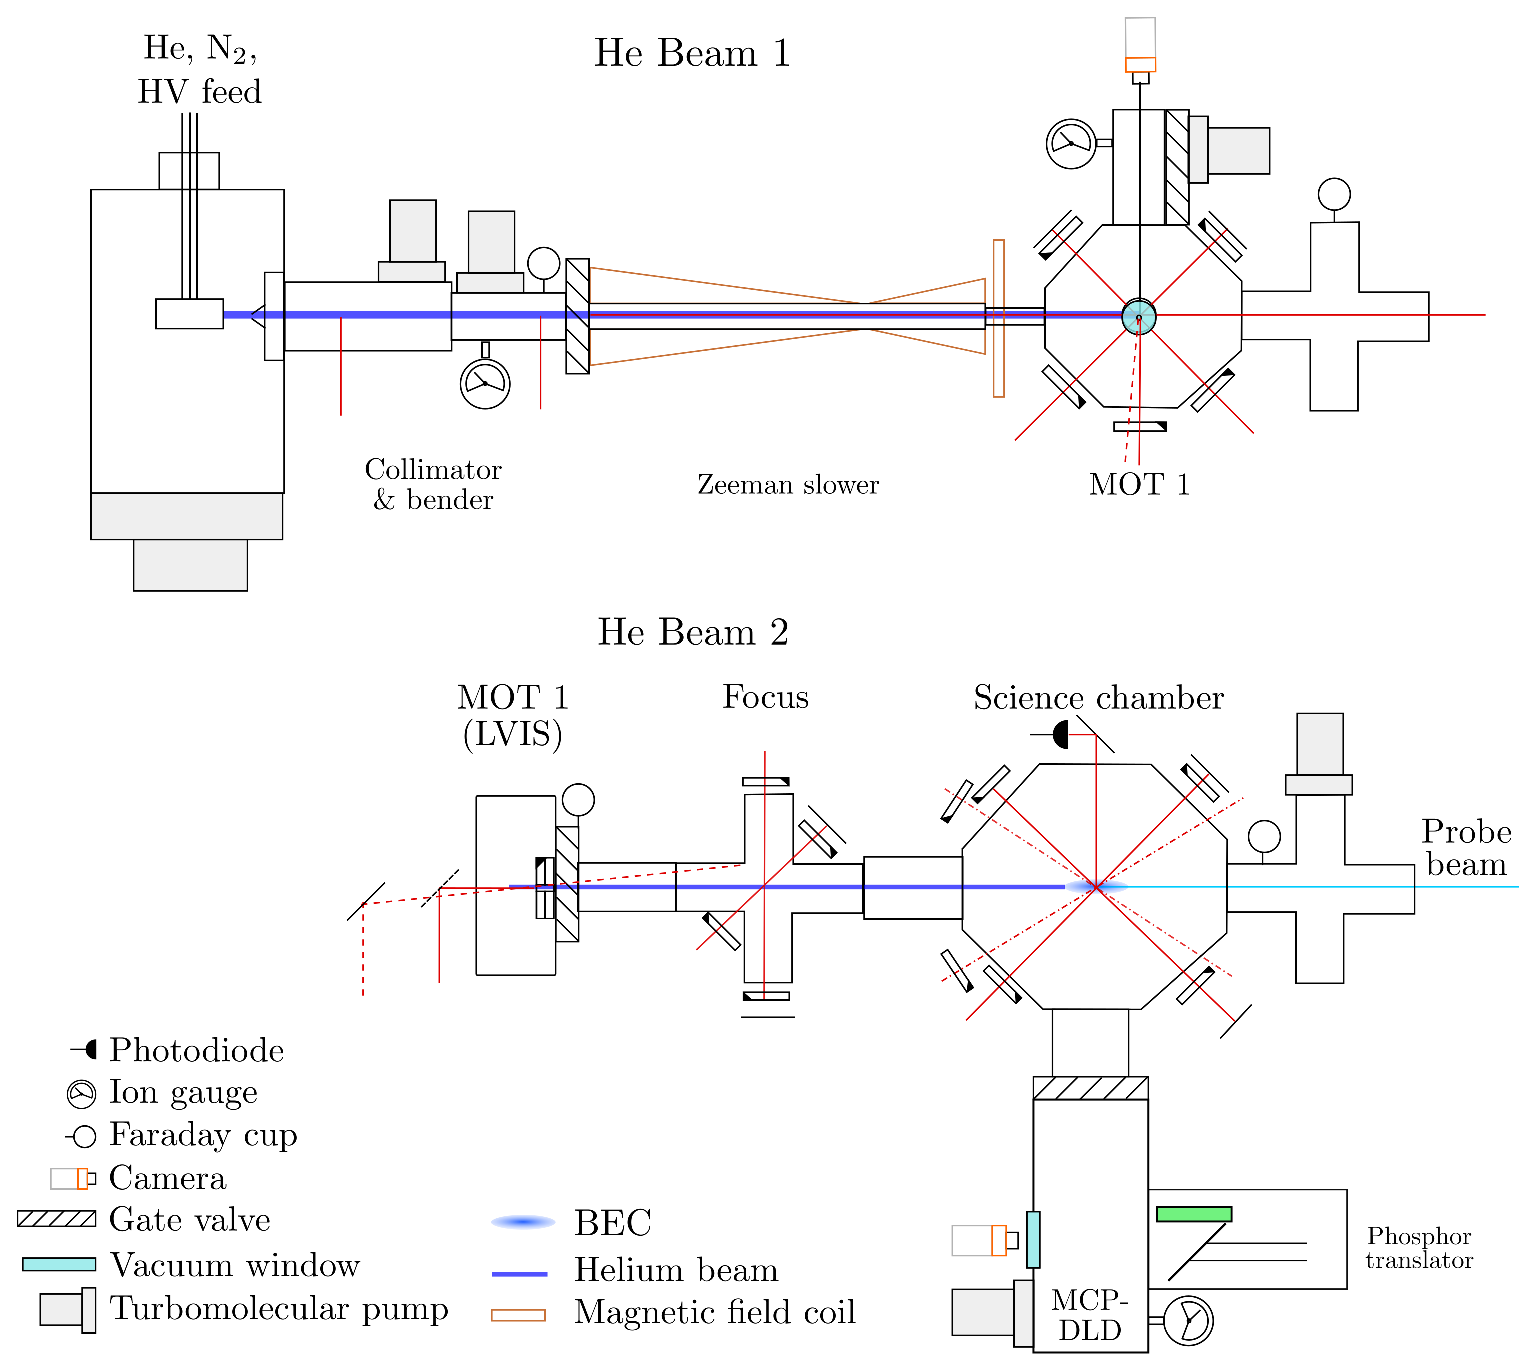
\includegraphics[width=\textwidth]{fig/apparatus/vacuum_schematic_simplified}
	% 	\caption{Vacuum system and laser insertion optics used in the BiQUIC machine.  The following features are not present in the lattice mahine: The spectroscopic laser (blue line) is inserted through a vacuum window along the weak ($x$) axis of the trap.  A phosphor-screen-backed MCP (green) is mounted above a 45$^\circ$ mirror permitting imaging of the phosphor pattern with a camera. This is typically used for troubleshooting and alignment rather than scientific purposes, and so is moved out of the fall-line with an in-vacuum translation mount.}
	% 	\label{fig:apparatus}
	% \end{figure}

	\begin{figure}
		\centering
		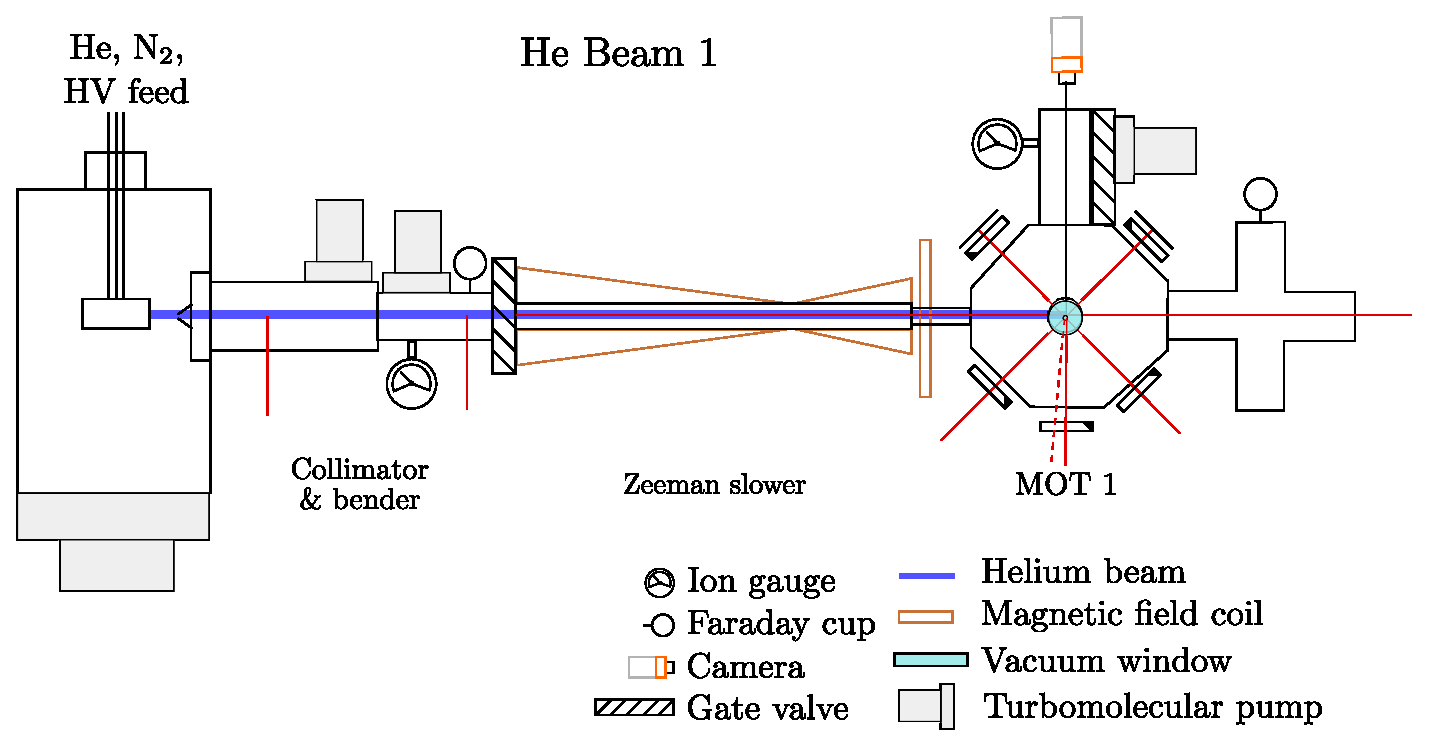
\includegraphics[width=\textwidth]{fig/apparatus/vacuum_schematic_split_1}
		\caption{Vacuum system and laser insertion optics for initial cooling of the helium from room temperature to the mK scale in the first MOT. The helium source is cooled by liquid $\textrm{N}_2$ and sustained by a high-voltage (HV) DC discharge.
		Cooling and trapping beams (solid red lines) are transmitted via free-space links from the AOM table and inserted through flange-mounted windows.
		The collimation and bending stage provide intial cooling and background reduction before feeding into the Zeeman slower, which reduces the longitudinal velocity of the atoms so they can be captured by the first MOT at the end of beam 1. 
		The horizontal beam in the first MOT is retro-reflected though a quarter-wave plate mounted on a mirror with a 2 mm hole bored through the centre, which feeds cold helium from MOT 1 into science chamber (see Fig. \ref{fig:apparatus_2})}
		\label{fig:apparatus}
	\end{figure}

	\begin{figure}
		\centering
		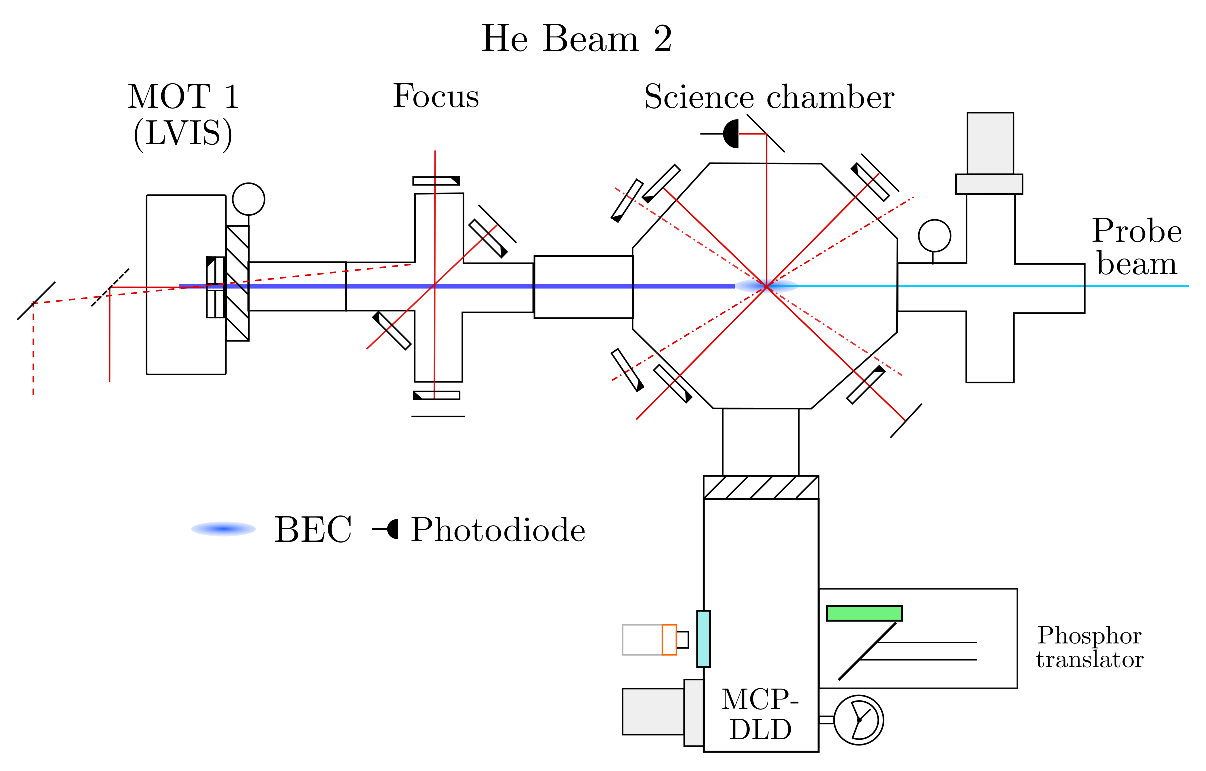
\includegraphics[width=\textwidth]{fig/apparatus/vacuum_schematic_split_2}
		\caption{Schematic of the second beamline. The low-velocity intense source (LVIS) of \mhe~ atoms is formed by kicking atoms from the first MOT into the ultra-high vacuum conditions of the science chamber with a slightly blue-detuned `push' beam. Doppler cooling beams (red dot-dash lines) lower the temperature before commencing evaporative cooling. Two other features are present in this diagram, and abesnt in the lattice machine. The spectroscopic laser (blue line) is inserted through a vacuum window along the weak ($x$) axis of the trap. A phosphor-screen-backed MCP (green) is mounted above a 45$^\circ$ mirror permitting imaging of the phosphor pattern with a camera. This is typically used for troubleshooting and alignment rather than scientific purposes, and so is moved out of the fall-line with an in-vacuum translation mount. }
		\label{fig:apparatus_2}
	\end{figure}
	

\subsection*{\mhe~atom source}

	The metastable \mhe~state is generally produced by a DC electric discharge as opposed to optical excitation due to the lack of convenient X-ray light sources at 63nm.
	Electrons accelerated by a strong potential gradient can ionize helium atoms, and thus also have enough energy to excite atoms into the \mhe~state (or achieve it by recombination and/or relaxation along a decay pathway including the $\MetastableState$ state).
	In our experiments, a grounded copper block cooled by liquid nitrogen serves as the anode and reaction vessel.
	A tungsten cathode is held at 2kV and placed in front of the vessel, separated by electrically insulating boron nitride spacers.
	The breakdown voltage of helium gas in this geometry is lowest at a pressure above the standard operating setting, and even then an additional 2.5kV pulse is required to achieve ignition before turning the source pressure down into the operating regime.
	Unfortunately, the DC discharge only excites about .01\% of the atoms into the \mhe~state \cite{Stas06}.
	Further, the light mass of helium means that even at temperatures around 70K (thanks to the liquid nitrogen cooling) the atoms have fairly high velocities necessitating a Zeeman slower stage before the initial trapping stage. 
	The source chamber tends to operate consistently over a year or so, permitting development and execution of a handful of experimental campaigns.
	However, the copper housing degrades with use.
	The first symptom of an ailing source is intermittent extinctions and, if not promptly addressed, an inability to successfully strike.
	This is remedied by extracting the source chamber from the vacuum system and skimming a few microns of material from the interior surface of the block, a procedure which is  straightforward but painstaking.
	

\subsection*{Beam forming}

	The gas expands out of the forward-facing aperture of the reaction vessel and a small solid angle is selected by a skimming nozzle between the source chamber and the rest of the helium beamline.
	The skimmer also functions as a differential pumping stage by rejecting atoms with large transverse velocities, and keeping the first laser cooling stages at a lower pressure than the source chamber.
	The beam is collimated by a single beam reflected in a figure-4 configuration (see Fig. \ref{fig:figure_4}), forming a a 2D optical molasses \cite{Lett81,Rooijakkers96} and providing cooling in the two transverse degrees of freedom.
	Before insertion into the chamber, a cylindrical lens expands the laser beam into an ellipse with a roughly 5:1 aspect ratio. The long axis is parallel to the helium beamline. The retro-reflection mirror (right of Fig. \ref{fig:figure_4}) is in fact a corner mirror which deflects the laser beam parallel to the helium beam before reflecting it back parallel to the incoming optical beam path.  
	This extends the interaction zone to about 10 cm. 
	The beams are offset in the image plane here for clarity, but in reality they are offset along the axis of the helium beam.
	In the schematic, the beam passes through the four-way intersection of the laser beams. 
	The laser detuning (red of resonance) ensures that only atoms moving against the laser propagation are Doppler-shifted towards resonance, hence reducing the beam divergence\footnote{Technically speaking, the beam is not collimated in the same manner as a laser beam.
	The divergence is reduced, but not eliminated such that the spot size remains fixed or becomes focused.}.
	% \begin{wrapfigure}{l}{0.5\textwidth}
	\begin{figure}
		\centering
		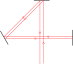
\includegraphics[width=0.5\textwidth]{fig/apparatus/figure_4_beams}
		\caption{Schematic of the figure-4 configuration used for transverse cooling of the source beam in the collimation stage. }
		\label{fig:figure_4}
	\end{figure}


	This is followed by a `bending' stage wherein a single beam, picked off from the collimator beam, deflects the metastable atoms by a few degrees through a second stage of differential pumping, which blocks the line of sight from the source to the MOT, into the Zeeman slower chamber.
	This provides better selectivity of \mhe~atoms by reducing the number of unexcited atoms that enter the Zeeman slower and first MOT chamber.
	% \subsection*{Optical molasses}
	% P D Lett, W D Phillips, S L Rolston, CE Tanner, R N Watts, C I Wetbrook, Optical Molasses, journal of the optical society of america B 6, 2084-2107, Nov 1981
	% W Rooijakkers, Wo Hogervorst, W Vassen, an intense collimated beam of metastable helium atoms by two-dimensional laser cooling, Optics COmmunications 123, january 1996

	Zeeman slowers, so named for the exploitation of the Zeeman effect\footnote{In the earier days of cold atom science they were sometimes called \emph{Zeeman-compensated slowers} \cite{Mastwijk98}}, are necessary to slow atoms from thermal characteristic of their sources to below the capture velocity of the magneto-optical traps located at the end of the slower.
	An atom moving with respect to a laser source (as described in section \ref{sec:doppler_basics}) in a magnetic field $\textbf{B} = B\hat{b}$ will have its electronic resonances shifted by the Doppler and Zeeman effects, which can be summarized as
	\begin{equation}
		\omega_{0,\text{lab}} = \omega_{0}\left(1 + \frac{k\cdot v}{c}\right) + \frac{\mu_B B}{\hbar}\left(g_e m_e - g_g m_g\right),
	\end{equation}
	where the $g$-factors and magnetic quantum numbers $m$ of the ground and excited state are denoted by $g$ and $e$, respectively. 
	Hence, a carefully architected magnetic field can compensate for the changing Doppler shift as atoms decelerate.
	The $\sigma^+$ light employed in our Zeeman slower drives the cooling transition with $g_g m_g = 2\times 1$ and $g_e m_e = \frac{3}{2}\times2$, leading to a field-dependent shift of $\approx1.4$ MHz/G.
	
	The magnetic field profile for maximum deceleration depends on the initial velocity, and so the spread of initial velocities according to the Maxwell-Boltzmann distribution necessitates another figure of merit to optimize against.
	In our experiments the Zeeman slower coil windings are built to create a field profile that maximizes the number of atoms slowed below the capture velocity of the first MOT \cite{Dedman04}.
	The Zeeman slower thus reduces the most probable longitudinal velocity of the beam from $\approx700$ m/s to $\approx70$ m/s, which permits loading of the MOT to a steady-state population in about one second.

	% W Rooijakkers, Wo Hogervorst, W Vassen, an intense collimated beam of metastable helium atoms by two-dimensional laser cooling, Optics COmmunications 123, january 1996

\subsection*{First Magneto-Optical Trap}
	% cooper94 temperature of atoms in a MOT
	The magneto-optical trap combines the radiation pressure with a spatially-varying magnetic field to confine atoms in three dimensions.
	Current-carrying coils in an anti-Helmholtz configuration create a locally linear magnetic strength (about the zero in the centre) with a gradient of the form $(B',B',-2B')$ where the stronger gradient is along the axis of symmetry. 
	Because the Zeeman shift of the levels in the helium $2\triplet S_1$ and $2\triplet P_2$ manifold are linear functions of the magnetic field strength (at least in regimes relevant to our traps, where the fine structure splitting of the $2\triplet P$ states is a thousandfold larger than the Zeeman shift), the cooling transition exhibits a Zeeman shift which is proportional to the distance from the centre of the trap.
	We drive the $\sigma^+$ transition between the $2\triplet S_1(m_J=1)$ and $2\triplet P_2(m_J=2)$ states, and red-detune the laser to ensure the light is resonant on an ellipsoidal shell around the trap centre.
	The atoms also exhibit a Doppler broadening from their motion within the trap, but this amounts to a broadening of $\approx100$ kHz at $\approx1$ mK, which is tiny in comparison with the $\approx 100$ MHz ($\approx 70\Gamma$) shift in the $1.6$ MHz-wide transition, a small correction to the picure just outlined\footnote{The Maxwellian distribution of velocities in a thermal cloud leads to a broadening of the absorption line due to the range of Doppler shifts experienced by the atoms. The Doppler-broadened linewidth can be calculated through $\Delta_{D} = \sqrt{8 k_B T\log(2)/(mc^2)}\omega_0$, where $\Delta$ is the broadened linewidth and $\omega_0$ is the resonant frequency \cite{FootAtomic}.}.
	The net result is that as an atom moves away from the origin of the trap, the probability of it absorbing a photon from the beam pointing back towards the origin increases, thus creating a restoring force along each axis.

	This technique was first proposed by Jean Dalibard and eventually realised by Raab \emph{et al} \cite{Raab87}.
	The population of early helium MOTs were limited because the small size of the trap and low detunings led to high densities and thus rapid deterioration by Penning losses.
	Later attempts achieved larger atom numbers by operating with larger beams and detunings (-22$\Gamma$), obtaining lower densities than in other species and mitigating losses due to Penning ionization \cite{Tol99}.
	The multifaceted physics of MOTs has proven rich ground for study in general \cite{Townsend95,Walker90}, and also in the specific case of helium, for which the two-body loss rate has been studied \cite{Tol99} along with the roles of light-assisted collisions \cite{Stas06,McNamara07}. 
	Temperatures in a MOT are, at best, on the order of the steady-state molasses temperature $\approx1$ mK \cite{Lett81}.
	Further evaporative cooling is therefore required to reach quantum degeneracy.
	
	The background pressure in the first MOT chamber is still too high to maintain a long-lived magnetic trap.
	Therefore, the first MOT is used as a source for a secondary helium beam which feeds into the science chamber.
	The MOT chamber features a $\approx$2 mm hole bored through a compound quarter-waveplate-and-mirror mounted inside the vacuum chamber (see Figs. \ref{fig:apparatus}\& \ref{fig:apparatus_2}), which adjoins the transfer conduit supplying the BEC chamber with cold helium.

	A slightly blue-detuned `push' beam is used to kick atoms through the aperture at the back of the first MOT into the second MOT along ballistic trajectories \cite{Swansson04}.
	In practise the beam points slightly upward, and the orientation is optimized by maximizing the saturated fluorescence signal in the second MOT (see section \ref{sec:he_detection}for a description of the technique).
	The atoms pass through a `focus' stage consisting of two crossed, retro-reflected laser beams with a $\approx$1 cm waist.
	Wire coils mounted around the (horizontal) 2$\frac{3}{4}$" window flanges create a quadrupole magnetic field surrounding the beamline such that the circularly-polarized beams address only atoms on the half of the beam proximal to the optical insertion.
	This final stage of transverse cooling increases the efficiency of loading the second MOT from the \mhe~beam.
	The focusing stage typically increases the saturated fluorescence signal in the second MOT by at least 50\%.
	

\subsection*{The Science Chamber}

	The second trapping chamber is evacuated to a pressure of some $10^{-11}$ mbar, yielding an excellent magnetic trap lifetime (permitting optical interrogation periods of up to 25 seconds after the $\approx$20 second BEC production sequence in one recent measurement \cite{Thomas20}).
	The chamber is surrounded by three pairs of square magnetic coils which actuate active cancellation of stray fields from the earth and nearby electronic equipment\footnote{The `nuller' reduces, but does not eliminate, 50Hz noise from the AC mains supply to the laboratory.} \cite{Dedman07}.
	This assists the creation of a stable magnetic trap with two coil pairs in a Bi-planar quadrupole Ioffe configuration (BiQUIC) \cite{Dall07}.
	These coils also generate the field which maintains the second MOT, wherein the final stage of optical cooling is provided by a pair of low-intensity Doppler cooling beams inserted at 15$^\circ$ relative to the horizontal \cite{Dall07_BEC}.
	The transfer between the two traps is achieved by simply switching off the light.


	Magnetic traps exploit the interaction between the atomic magnetic dipole and a magnetic field, taking the form $E_B = -\mu\cdot \textbf{B} = -\hbar g m_J B$.
	A magnetic field with a local extremum can therefore form a confining potential for the states whose energy is minimized at this point.
	It follows from the Earnshaw's theorem that a magnetic field in free space cannot have any local maxima \cite{Harms00,MakingProbingUnderstanding}, and so one must select an atomic state with $g m_J>0$ for confinement at a local minimum of the magnetic field strength.
	In \mhe~this uniquely selects the $m_J=+1$ state for magnetic trapping, which also ensures complete spin-polarization and the attendant reduction in Penning losses.
	The BiQUIC design is a solution to a critical issue with early traps \cite{Migdall85}: The quadrupole fields generated by coils in an anti-Helmholtz configuration feature a zero crossing in the trap centre.
	Atoms in a magnetic field undergo transitions to untrapped states, known as \emph{Majorana transitions}, at a rate proportional to $\exp(-B/\omega)$, where $\omega$ is the trapping frequency and $B$ is the magnitude of a (uniform) magnetic field \cite{Sukumar97}.
	In harmonic traps the Zeeman splitting at the trap minimum thus sets the upper bound on the Majorana transition rate \cite{Brink06}.
	Many variations on the quadrupole trap exist to mitigate this issue, including the Time-Orbiting Potential (TOP) \cite{Petrich95}, Ioffe-Pritchard \cite{Pritchard83}, cloverleaf \cite{Mewes96}, and QUIC \cite{Esslinger98} traps, while other groups have added a repulsive dipole potential to the trap zero with a focused and blue-detuned laser beam \cite{Davis95}.
	The magnetic trap enables forced evaporative cooling to below the condensation threshold, some three orders of magnitude colder than the limits of optical cooling. 


  

	\begin{figure}
	\begin{minipage}{0.55\textwidth} %4-8-16
	\vspace{0pt}
		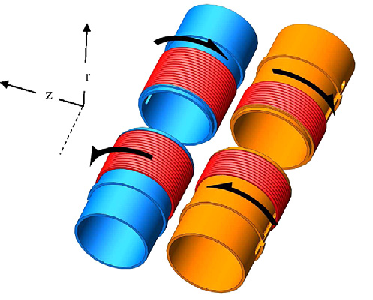
\includegraphics[width=\textwidth]{fig/apparatus/biquic_coil.pdf}

	\end{minipage}
	\hfill
	\begin{minipage}{0.45\textwidth}
	\vspace{0pt}
	\caption{Schematic diagram of the Bi-QUIC coil design. Black arrows indicate the direction of current flow. The cylindrical coordinate axes indicate the axis of symmetry ($z$), which has a lower trapping frequency (O(40) Hz) than the `tight' axes (O(400) Hz). Diagram reproduced with permission from \cite{Dall07}}
	\end{minipage}
	\end{figure}

	A comprehensive introduction to evaporative cooling can be found in \cite{Ketterle96}; see \cite{FootAtomic,PethickSmith} for more compact discussions. 
	Here I present a short, intuitive picture of evaporative cooling in a semiclassical, non-interacting model. 
	A gas of bosons at finite temperature will consist of atoms whose energies are described by Bose-Einstein statistics (see chapter \ref{chap:theory}). 
	At equilibrium, the expected population of single-particle states falls off exponentially with energy $E$. 
	Therefore there will be some atoms which have much greater energy than the average. 
	If these atoms are confined in a magnetic trap, then the more energetic atoms will be more likely to be found further from the trap origin.
	The wavefunction of the high-energy atoms will thus be supported in regions with larger magnetic fields than the lower-energy atoms.
	Therefore it is possible to selectively remove the high-energy atoms by driving the transition between trapped and untrapped states with radio-frequency (RF) radiation tuned to the resonance near the Zeeman splitting seen by only the most energetic atoms in the trap.
	After a timescale on the order of a few times the (inverse) inter-atomic collision rate, the gas rethermalizes (i.e. regains the Bose-Einstein statistics after having its tail cut off) at a lower temperature by virtue of losing its most energetic constituents.
	Repeating this process for lower RF frequencies removes atoms with progressively lower energies, cooling the sample.
	If one ramps the radio frequency down too quickly, then the loss rate of atoms can counteract the loss of temperature and result in a decrease in phase-space density, i.e. moving further from the condensation threshold.
	Conversely, a ramp that is slow will be more efficient but also more subject to other trap loss channels and needlessly prolong the experimental cycle.
	Theoretically optimal evaporative cooling ramps are discussed in \cite{Ketterle96}, and in practise we apply a continuous RF sweep from 20 MHz down to $\approx800$ kHz, with an empirically-optimized and roughly exponential shape over about 20 seconds.
	The endpoint of the ramp depends on the configuration of the BiQUIC trap (specifically the trapping frequency and the bias at the trap centre) and the desired size and temperature of the condensate. 
	


	Two radio antennas provide the RF signals for evaporative cooling and atom lasers, respectively.
	The evaporative cooling ramp is generated by an arbitrary waveform generator pre-loaded with a time-varying frequency ramp created with the LabView control software (see section \ref{sec:DAQ}).
	The secondary coil is driven by a function generator according to a waveform that is pre-loaded at the start of the experimental sequence.
	Both signals are passed through separate dedicated 30W amplifiers before insertion into the chamber.
	A vacuum window on the opposite side to the helium beam provides optical access for a spectroscopic probe beam or the 1550nm beams used for atom-optics techniques (employed in works not relevant to this thesis).
	The final relevant component is a diagnostic photodiode mounted outside the chamber and is used to measure a saturated fluorescence signal (see section \ref{sec:he_detection}), which serves as a diagnostic for the in-trap population.


\section{Light sources}\label{ssec:lasers}
\subsection*{Cooling and trapping light}
	
	\begin{figure}
		\centering
		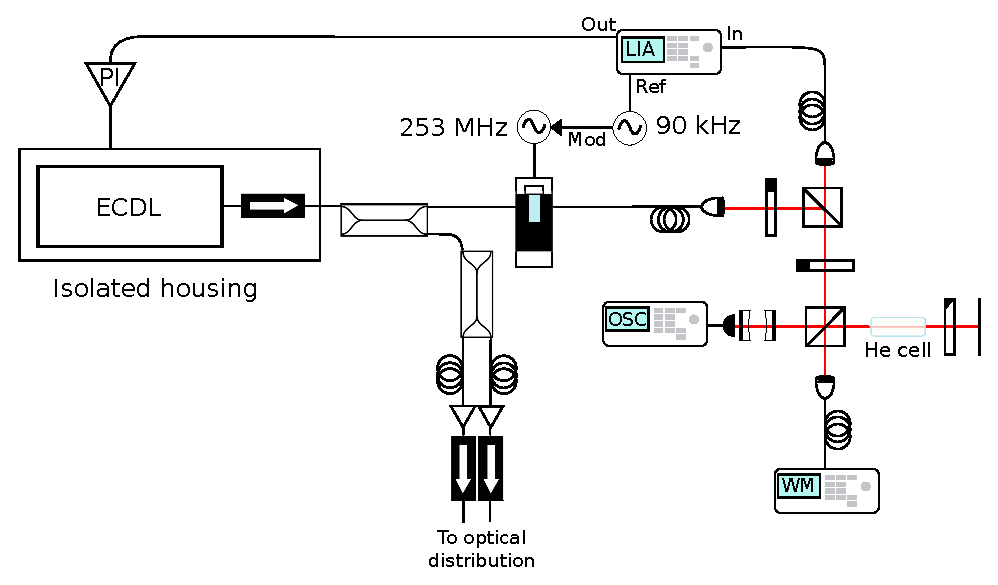
\includegraphics[width=\textwidth]{fig/apparatus/master_laser_system}
		\caption{Schematic of the generation and control system for the main cooling laser operating at 1083.331nm described in the text. Light from the laser diode is filtered by the cavity resonance and internal diffraction grating, which is actuated by a piezoelectric crystal. Part of the light is picked off with an in-fibre beamsplitter and sent to the experiments. The rest passes through an in-fibre AOM which increases the frequency by 253 MHz and outputs light into the saturated-absorption spectroscopy system (lower right). The SAS offset is in turn modulated at 90kHz and the demodulated signal (output of the LIA) is proportional to the gradient of the SAS signal, which is minimized at the absorption peak. Hence the demodulated output serves as the error signal for a PID controller that feeds back to the piezoelectric actuator of the frequency-selective diffraction grating. Further details about the spectroscopy technique can be found in \cite{ShinThesis,FootAtomic}.}
		\label{fig:main_laser}
	\end{figure}
	
	
	The principal light source for both machines is the 1083.331nm cooling and trapping laser.
	The light source, depicted in Figure \ref{fig:main_laser}, is an external-cavity diode laser (ECDL) that operates with a locked linewidth below 100kHz and is detailed in the publication \cite{Shin16} and in PhD thesis of D. K. Shin \cite{ShinThesis}.
	The output of the ECDL passes through an in-fibre beamsplitter, from which one output is blue-shifted by 253MHz by an acousto-optical modulator (AOM) and locked to a helium gas cell by saturation absorption spectroscopy.
	The remaining arm is coupled by optical fibres to the fibre amplifiers of both experiments.
	Each experiment features its own fibre amplifier that produces up to 5 Watts of laser power from the $\approx$3 mW supplied by the ECDL and then distributes the light to the laser cooling and trapping chambers via a suite of dedicated AOMs (depicted in section \ref{sec:new_optics}).

	
	% N Herschbach, Trrapped Triplet helium atoms: inelastic collisions and evaporative cooling, PhD thesis VU Amsterdam 2003


	% http://www.heliumbec.com/wiki/February_2017_Bake
	% https://imgur.com/a/4BxKh
	% http://www.heliumbec.com/wiki/Titanium_Sublimation
	% \begin{figure}
	% 	\centering
	% 	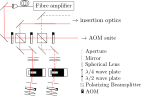
\includegraphics[width=0.6\textwidth]{fig/apparatus/distribution_optics}
	% 	\caption{Partial schematic of the control and distribution system for cooling light in the lattice machine. The fibre amplifier supplies light to each of several AOMs in cat's-eye configuration (two shown, one marked with dashed beamline). Half-wave plates control the optical power supplied to each AOM via polarizing beamsplitters. Pairs of mirrors permit alignment through a focus lens into the AOM crystal. The first diffracted mode is spatially selected by an aperture on the outgoing side, which is reflected and re-focused by a lens of equal focal length. A quarter-wave plate ensures that the the polarization is rotate from H to V after the second pass through the AOM hence is transmitted through the beamsplitter and then to the beam-forming optics before insertion into the vacuum chamber. }
	% 	\label{fig:distribution_optics}
	% \end{figure}

	In each machine, a suite of AOMs are used to independently control the power and frequency of each of several specialized beams\footnote{The active component of an AOM is a crystal is driven at radio frequencies by an amplified voltage-controlled oscillator.	An acoustic standing wave, constituted by phonons with frequency matched to the driving frequency, scatters light into discrete diffraction modes width momenta shifted by the phonon-lattice momentum.	The action is analogous to a diffraction grating, and described by the Kapitza-Dirac mechanism.	Thus the AOM transduces electronic signals into optical frequency shifts.	An analogous effect, with the role of atoms and light interchanged, is the operating principle of optical lattices.}.
	The AOM suites are supplied by light picked off from the output of the fibre amplifier by a half-waveplate and beamsplitter pair per AOM.
	The first-order diffraction is usually chosen for its more efficient transmission.
	The pointing of the diffracted beams vary with the AOM frequency, which is a problem when the ultimate destination of the light is separated from the AOM by several meters of optical path length, after which the deflection can become significant.
	To circumvent this, the AOMs are set up in a double-pass `cat's-eye' configuration so the deflection in one pass is canceled by the second pass in the opposite direction.
	A quarter-wave plate placed in the optical path through the cat's-eye ensures the doubly-diffracted beams are transmitted back through the beamsplitter into the distribution optics.
	
	AOMs offer the advantage of fast switching times, but some light can leak from the AOM suite through the optical paths into the vacuum chamber.
	As such we used electronic shutters and an opaque enclosure to prevent this from occurring.
	The shutter action as well as the detuning and diffraction efficiency of the AOMs are actuated by the control software described later in this chapter.
	
	The supply of light which is 253MHz red of the field-free resonance reduces the risk of stray light interacting with atoms and disrupting the delicate cooling and trapping processes.
	Furthermore, the fact that AOMs are limited in operation to a maximum frequency on the order of a hundred MHz or so means that the large detunings required for certain laser cooling applications could not be achieved using such double-pass setups seeded by resonant light\footnote{Cascading double-pass systems are certainly possible, but adding more moving parts with efficiencies generally below 80\% is undesirable.}.
	The lattice machine also makes use of 1550nm light for trapping in an optical dipole (and eventually lattice), whose generation and application is discussed in chapter \ref{chap:lattice}.	


	
	

\subsection*{Spectroscopic laser}
%mark
\label{sec:spec_laser}
	\begin{figure}
		\centering
		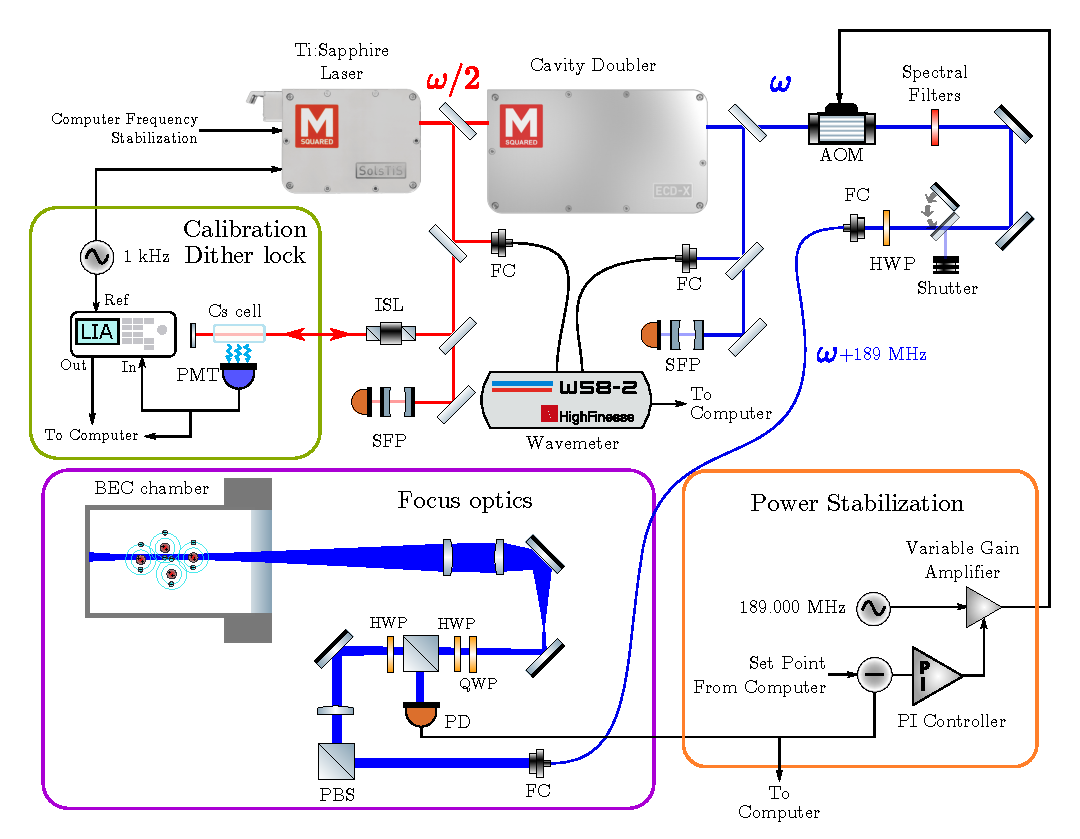
\includegraphics[width=\textwidth]{fig/apparatus/exp_optics_schematic}
		\caption{Schematic of the spectroscopic laser system.  The main laser modules supply light through an optical fibre, after three stages of optical filtering, to the insertion optics. The input to the fibre is the first diffraction mode from the AOM that serves as the actuator for an electronic PID loop whose power set point (P set) is compared to the reading of a photodiode (P act) at the insertion optics. The laser frequency is stabilized by a software-based PID loop that actuates the Ti:S cavity length (via inboard piezos) to reduce the between the desired and actual wavelengths ($\lambda$ set and $\lambda$ act, resp.). A pair of scanning Fabry-Perot cavities (SFP)  monitor the light from each laser module to verify both are operating in a single-mode regime. The switches at the input to the Ti:S are shown in the configuration used to calibrate the wavemeter. In this procedure the flipper mirror (coupling red light to the SFP) is removed and light enters a cesium gas cell. The fluorescence signal is measured by a photomultiplier tube backed by a photodiode, and this provides the signal for a dither lock at 1 kHz, demodulated by a lock-in amplifier (LIA).}
		\label{fig:tunable_laser}
	\end{figure}

	A light source unique to the BiQUIC machine was the tunable laser system used to generate light in the $402-430$nm range for laser spectroscopy (namely the works \cite{Ross20,Henson22} corresponding to chapters \ref{chap:transitions} and \ref{chap:tuneout} respectively, and also Ref. \cite{Thomas20}).
	This laser system is depicted in Figure \ref{fig:tunable_laser}.
	Light at 1064nm from a Lighthouse Photonics \emph{Sprout} module was frequency doubled by second-harmonic generation to pump an M-squared SolsTi:S titanium-sapphire laser which we operated around 800nm.
	The output from the SolsTi:S was doubled again in an M-squared ECD-X module to the target wavelengths.
	A fraction of the light is fed into a High Finesse WS-8 wavemeter.
	A MATLAB software lock uses the wavemeter output to stabilize the laser to within 100 kHz of the target wavelength, and allows automatic scans across the region of interest by automatically updating the laser set point (details are provided in section \ref{sec:DAQ}).
	We use the wavemeter to lock the tunable laser with respect to the red light, so the instrumental uncertainty is doubled in determinations of the blue frequency.
	High Finesse specifies the absolute accuracy of the WS-8 at 2 MHz within 2 nm of a transition line, and 10 MHz otherwise.
	We calibrated the wavemeter once every day or so with respect to the two-photon crossover transition between the $6^2P_{\frac{3}{2}} (F=4)$ and $6^2P_{\frac{3}{2}} (F=5)$ lines in a cesium vapor cell.
	We used saturated absorption spectroscopy to lock the red light to the Cs transition while feeding light into the wavemeter for the calibration.	
	

	We used the first diffracted mode of an AOM, driven at 189 MHz, to control the beam power.
	The output of the AOM was fed into an optical fibre which coupled the light to the vacuum insertion optics.
	{After exiting the fibre, the light was linearly polarized and a small fraction was directed onto a photodiode, whose voltage served as the input parameter to a PID loop.
	The control loop had a 3dB bandwidth of 170 kHz and was able to stabilize the beam power to within a relative error of 0.3\%.}
	There, we used waveplates to set the polarization and a telescope to magnify the beam up to $\approx$2 cm waist.
	A final lens fixed to a three-axis translation mount was used to focus and align the beam.
	For the measurements of the tune-out and forbidden transition wavelengths, we focused the beam to a $\approx10~\mu$m diffraction-limited waist at the site of the BEC to achieve strong interaction given the weak signals of interest.
	For the $2\triplet P_2\rightarrow 5\triplet D$ transitions described in chapter \ref{chap:transitions}, the beam was collimated and operated at a reduced power to mitigate power broadening and saturation of these much stronger resonances.
	The optical power was regulated with reference to a photodiode that sampled the beam after the fibre via a polarizing beamsplitter.

	The wavemeter logs, photodiode voltage, and transmission of light from both the red and blue beams through two scanning Fabry-Perot cavities (SFPs) were recorded through the DAQ system in order to provide diagnostics in post-processing.
	Part of the data analysis pipeline then automatically discarded shots where either SFP showed multiple peaks within a single free-spectral range (FSR), indicating that one of the lasers was running in a multimode regime, or where the photodiode trace indicated a laser supply failure, or where other anomalous behaviour was detected.

% \rem{\subsubsection{Wavemeter Calibration}
% 	To provide an absolute calibration of the wavemeter we use the Doppler-free two-photon $6^{2}S_{1/2} (F=3) \rightarrow 8^{2}S_{1/2} (F=3)$ and $6^{2}S_{1/2} (F=4) \rightarrow 8^{2}S_{1/2} (F=4)$ transitions in cesium around 364.5~THz (822.5~nm). We split off a small fraction ($\sim$50~mW) of the red light generated by the Ti:Sapphire laser (before the doubling cavity), pass it through a warm (50$^{\circ}$~C) cesium cell with a beam waist of $\sim0.5$~mm, and then reflect it backwards along its path.
% 	We detect the excitation of the transition using the blue florescence from the radiative cascade \cite{Hagel99}, with a blue-sensitive (red-blind) photomultiplier tube (PMT). Previous measurements \cite{Wu13,Fendel07} have precisely measured the $F=3\rightarrow3$ and $4\rightarrow4$ transitions to be 364\,507\,238.363(10) and 364\,503\,080.297(10) MHZ respectively, and have demonstrated an insensitivity to environmental conditions, which makes these transitions suitable as a secondary frequency standard. 

% 	To calibrate the wavemeter we disable the usual software based wavemeter feedback to the laser and instead stabilize the laser using one of these transitions. To produce a derivative error signal suitable for feedback we modulate the frequency of the Ti:Sapphire laser (frequency deviation $<50$~kHz, modulation frequency $\sim1$~kHz) and detect the resulting modulation in the PMT current with a lock-in amplifier. This analog error signal is continuously read by a software based PID controller which sends adjustment commands to the laser controller (rate $\sim20$~Hz) to maintain the the laser frequency at the maximum of the fluorescence.

% 	As a verification of the calibration procedure we then re-engage the wavemeter based laser feedback system and measure the PMT current as a function of the frequency set point. We fit these data with a Lorentzian profile to extract the transition frequency and verify the calibration procedure (see Fig.~\ref{fig:2p_scan_single}). After calibration we find that measurements of both $F=3\rightarrow3$ and $F=4\rightarrow4$ transitions give frequencies within 50~kHz of the reference values.
% 	Calibrations are carried out every few days as the ($\sim100$~mK) temperature stability of our laboratory reduces the thermal drift of the wavemeter.
% 	Based on previous systematic studies of these transitions \cite{Wu13,Fendel07} and the conditions used for calibration, we believe that the systematic error of this calibration procedure ($<100$~kHz) is well below the absolute accuracy of the wavemeter over the measurement range used in the this work (2~MHz within 3~THz (2~nm) of calibration \cite{wstechnical}). As the wavemeter measurement and calibration is carried out on the red side of the laser system before the doubling cavity the absolute accuracy of the frequency of the delivered (blue) light is doubled to 4~MHz, well below other systematic uncertainties.

	% references for 2p transtion
	% https://www.osapublishing.org/ol/abstract.cfm?uri=ol-32-6-701
	% https://www.osapublishing.org/ol/abstract.cfm?uri=ol-30-24-3413
	% https://www.sciencedirect.com/science/article/pii/S0030401898006622?via%3Dihub#FIG3
	% https://www.osapublishing.org/ol/abstract.cfm?uri=ol-38-16-3186


	% \begin{figure}
	%     \centering
	%     \includegraphics[width=0.6\textwidth]{fig/tuneout/2p_scan_nice}
	%     \caption{(Top) single scan of PMT current vs. optical frequency relative to the two photon transition $6^{2}S_{1/2} (F=3) \rightarrow 8^{2}S_{1/2} (F=3)$. A Voigt fit is shown as the black line for comparison, with fit parameters are $\sigma=0.18(3)$~MHz $\gamma=0.49(3)$~MHz. This scan took a total of \(75\)~s. (Bottom) Residuals of the fit model, where the shaded region is the standard deviation of the observation error model. 
	%     }
	%     \label{fig:2p_scan_single}
	% \end{figure}}
	% Camera/mirror setup Reproducibility
	% issues

\section{Detection of metastable helium atoms}
\label{sec:he_detection}
	Two optical detection methods are employed in the ANU helium labs.
	Resonant absorption imaging is only used in the lattice machine, and is therefore discussed in chapter \ref{chap:lattice}.
	Both machines make use of saturated fluorescence measurements to measure the number of atoms in a trap.
	In this method, bright resonant light ($I\gg I_\textrm{sat}$) is applied to the atoms such that the population of the excited state saturates at 50\%.
	If the light is applied while the trap remains on, then while some atoms may decay to a trapped state, repeated absorption events eventually drive them out of the trap.
	Therefore, one expects a sharp peak and subsequent decay in the optical power re-emitted from the trap.
	This radiation can be captured by a lens and focused onto a photodiode, producing an analog voltage which can be used to measure the number of atoms confined in the trap.
	The difference between peak and steady-state voltage after the pulse is a direct probe of the atomic population (see chapter \ref{chap:lattice} for further discussion).
	This technique is employed as a diagnostic tool for fast readout of the second MOT population when optimizing the alignment of cooling and trapping beams. 

	A unique diagnostic available in helium experiments is the production of helium ion-electron pairs.
	This process can be monitored by in-vacuum electron multipliers mounted near the trapping region.
	Proximity to the trap is desirable for efficient collection of the resulting particles.
	Aside from investigating Penning ionization itself, ion detection has been applied in photoassociation spectroscopy \cite{Herschbach00,Koelemeij04}, to monitor the onset of Bose-Einstein condensation \cite{Tychkov06}, and for high-precision laser spectroscopy \cite{Rengelink18}.
	Ion detection garners only a brief mention in works relevant to chapter \ref{chap:lattice}, wherein we hoped to detect ions as a diagnostic when aligning an optical dipole trap\footnote{The ion detector in the BiQUIC machine stopped working some years ago and has not been replaced: the utility of this diagnostic is outweighed by the effort required to break vacuum for the first time in a decade or so, disassemble the chamber and surrounding optics, reassemble everything, bake the chamber, and realign all the optics.}.
	In an accident a year or so after I left that lab, a ceramic feed-through connecting the ion detector to the external electronics cracked.
	This broke vacuum, necessitating a rebake of the chamber, and saw the detector retired.
	


\subsection*{Single-atom detection with the MCP-DLD stack}
	\label{sec:DLD}
	% http://www.heliumbec.com/wiki/Detectors
	The principal detection scheme in this thesis is single-atom sensing in the far-field regime using a multichannel plate and delay-line detector combination (MCP-DLD)\footnote{In this context far-field means that the density of the cloud is determined by the initial velocity distribution and that effects of the finite initial size are negligible. This is suitable in our experiments because the condensate is smaller than the detector resolution. See chapter 5 of D. K. Shin's PhD thesis \cite{ShinThesis} for a quantitative discussion.}.
	

	\begin{figure}
		\centering
		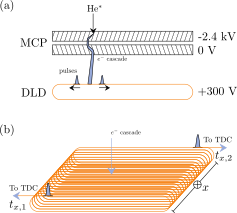
\includegraphics[width=\textwidth]{fig/apparatus/mcp_dld_schematic}
		\caption{Schematic sketch of the MCP-DLD detector. The twin plates of the multi-channel electron multiplier (MCP) have a 2.4kV potential between the upper and lower surfaces which accelerates electrons along the pores after they are freed from the surface by the energy released from \mhe~impact events. The resultant shower of electrons deposits a charge excess on a winding of the delay-line detector (DLD), which disperses as oppositely-travelling current pulses along the line. The arrival times ($t_{i,1}$ and $t_{i,2}$) of each pulse along each axis are received by the TDC and used to infer the respective coordinate of the electron cascade (only the winding along $x$ is shown for simplicity, but in the BiQUIC machine the DLD consists of two orthogonal windings).}
		\label{fig:MCP_DLD}
	\end{figure}

	In some configurations, such as the one at the \mhe~group at VU Amsterdam, the MCP itself can be used as an ion- or metastable-atom detector.
	In our machines, the MCP is paired with either a phosphor screen (usually only used for diagnostic purposes) or more typically with a delay line detector to form the MCP-DLD that is the workhorse of most experiments conducted at ANU.
	A summary description is given here, and detailed explanations of the detector stack and signal processing pipeline can be found in \cite{ShinThesis, HodgmanThesis, ManningThesis}.
	The MCP consists of two plates, each of which feature 10 $\micron$-diameter pores arranged in a square grid with 20 $\micron$ between the centres of the pore openings.
	The plates are 80 mm in diameter, with the upper surface 848 mm below the BiQUIC trap centre.
	The freefall time-of-flight of the centre of mass of the cloud is 417 ms, and so the maximum detectable horizontal velocity is about 9.5 m/s, sufficient to capture almost all of the thermal fraction for clouds below the critical temperature.
	The detector plates are grounded for most of the experimental sequence, and then the top plate is ramped to $-2.4$ kV over about 2 seconds before dropping the trap.
	The negative voltage repels electrons from the surface of the plate, protecting the detector surface from degradation and reduces the background count rate.
	The background rate, also called the \emph{dark count} rate, is typically 0.56 Hz/cm$^2$ when operating the plates at $-2.4$ kV, and is negligible for the purposes of experiments in this thesis.
	

	When an atom strikes the surface of a pore after falling from the trap, a second-order process releases a free electron with most of the 19.8 eV as kinetic energy \cite{Jagutzi02,Hotop96}.
	These electrons are accelerated down the pore by the strong electric field, and themselves impact the pore surface and eject more electrons, triggering an electron avalanche that amplifies each atom impact into over 10$^6$ electrons.
	The electron shower exits the back of the detector and is accelerated by a +300V potential towards the delay-line detector (DLD).
	The DLD in the BiQUIC machine consists of two coils of wire each wound in a helical pattern and arranged perpendicular to one another.
	 The arrival of an electron cascade causes a current pulse to travel along each wire in both directions from the point of impact.
	The pulses pass through a fast pre-amplifier and then through a constant-fraction discriminator which converts the analog pulses into a digital signal.
	Both of these processes take place within a Roentdek DLATR6 which is located outside the vacuum chamber.
	The digital pulses are transmitted to a Roentdek TDC8HP time-digital converter (TDC) which registers the arrival times, relative to the arrival of the main trigger signal from the LabView control software, and writes these to a \verb|txt| file as \verb|(channel,time)| pairs.
	Finally, a custom C++ script passes over the file and converts the timing data to \verb|(t,x,y)| tuples.
	The conversion from \verb|(channel,time)| to \verb|(t,x,y)| is performed separately, and indeed the latter usually by a different machine, so as to provide maximum CPU availability to the acquisition function.	Further details about the architecture, construction, and calibration of these detectors is found in \cite{HodgmanThesis,ManningThesis}.

	A second MCP, backed by a phosphor screen and a mirror at 45$^\circ$ to the vertical axis, is mounted on an in-vacuum translation stage below the main chamber.
	The mirror directs light from the phosphor screen to a CCD camera mounted outside the vacuum chamber.
	This detection method is not typically used for scientific purposes these days, but is a useful additional diagnostic when the MCP-DLD detector stack appears to be faulty.
	The phosphor screen does have a much larger dynamic range than the DLD, however, which makes it useful for visual spotting of subtle distortions in the BEC profile, such as used in the alignment of the spectroscopic probe beam.
	


	% % NTM [185] derivation of detector flux profiles - inc mean field 
	% % % Tychkov PhD thesis
	% % RGL [98] calibration of QE - depends on plate voltage, which in turn affects plate lifetime and rate of degradation of QE 
	% % % van Rooij PhD thesis
	% % RGL MCP flux models [94] inc BEC flux in terms of chemical potential 
	% % % van Rooij PhD thesis
	% % TKV [9,10] expanding condensate density distributions 
	% % % Y Castin, R Dum, bose-einstein condensation in time-dependent traps, Physical Review Letters 77, 1996
	% % % F Dalfovo, S Georgini, L P Pitaevskii, S stringari, theory of bose-einstein condensation in trapped gases, rev mod phys 71, april 1999
	% % SSH [38,39] condensate ballstic expansion 
	% % % Castin & Dum
	% % % K.
	% Dieckmann, Bose-Einstein Condensation with High Atom Number in a Deep Magnetic Trap, Ph.D.
	% thesis, University of Amsterdam (2001).

		 % \newpage
	 \begin{figure}
	 	\centering
	 	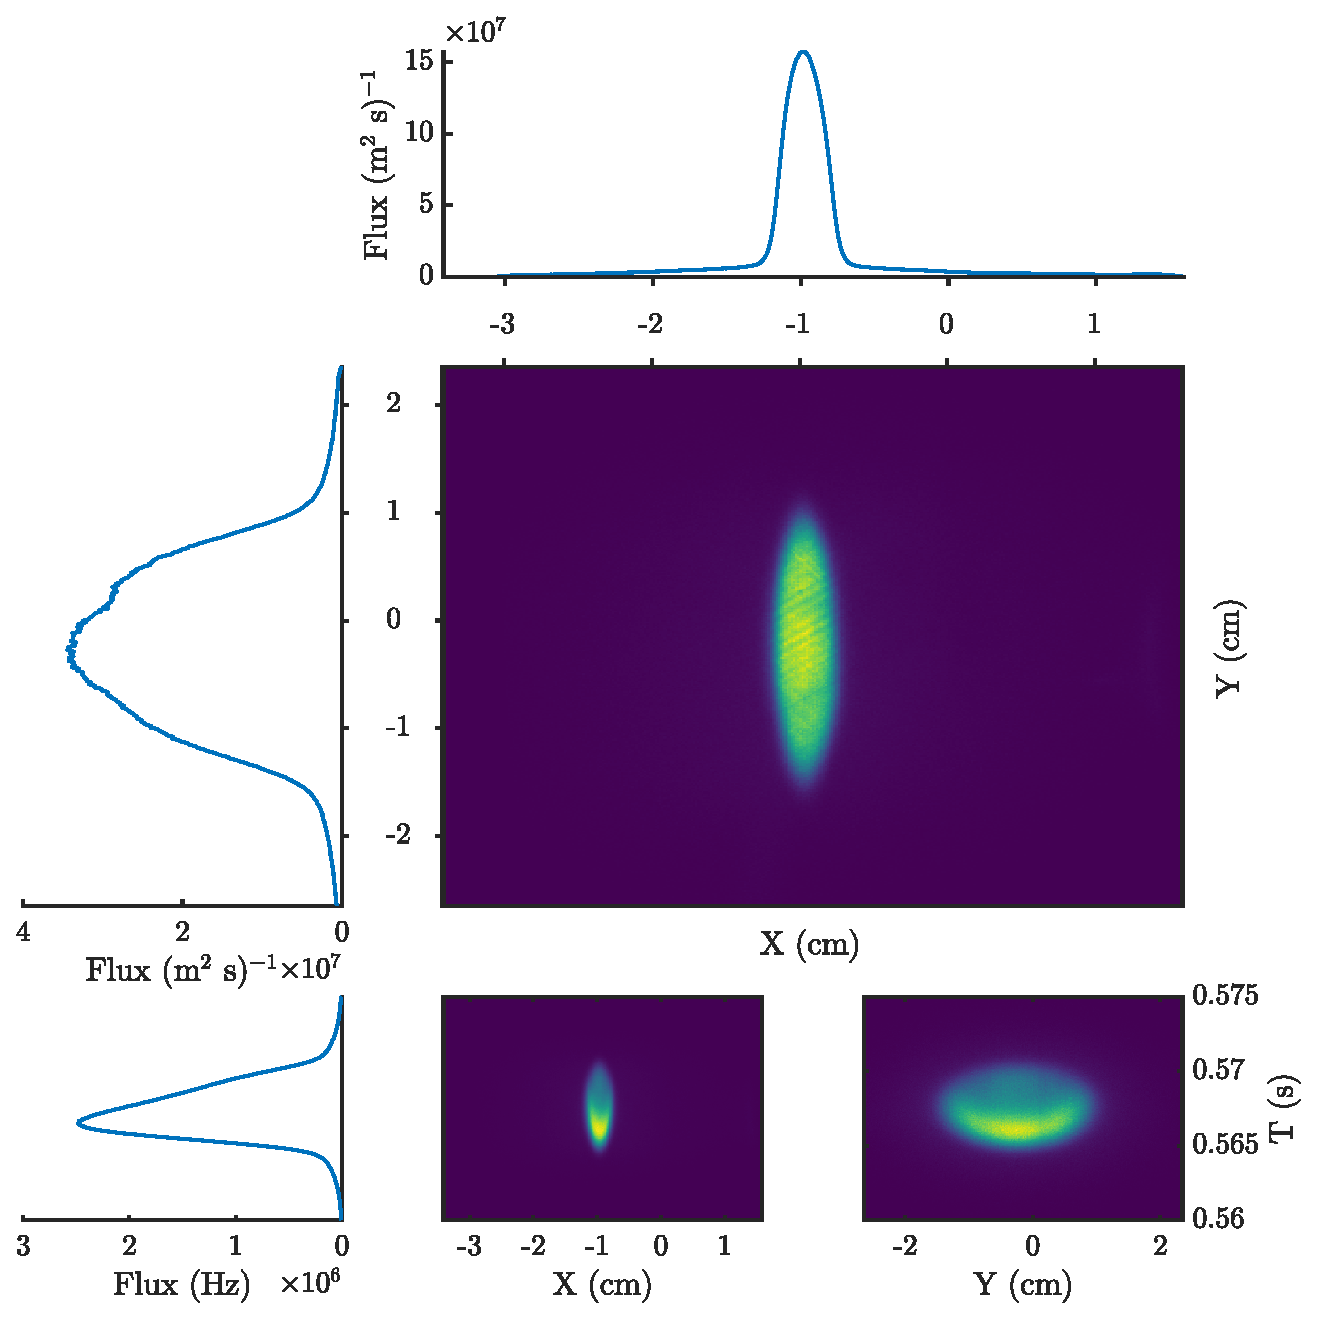
\includegraphics[width=\textwidth]{fig/apparatus/dropped_bec}
	 	\caption{MCP readout of a dropped BEC with small thermal fraction, just visible as dilute wings outside the central peak.
		The detector saturation is evident in the time-of-flight profiles (bottom row, all with common vertical axis) as a sudden downturn in the detected flux, whereas the full BEC has a parabolic profile.
		The density- and space-dependence of the saturation is visible in the 2D sections (lower middle and lower right). The one-dimensional fluxes along X and Y are averaged over the time interval displayed in the bottom row, and the total count rate (bottom left) is integrated over the entire detector.}
	 	\label{fig:dropped_bec}
	 \end{figure}

	 \newpage
	 \begin{figure}
	 	\centering
	 	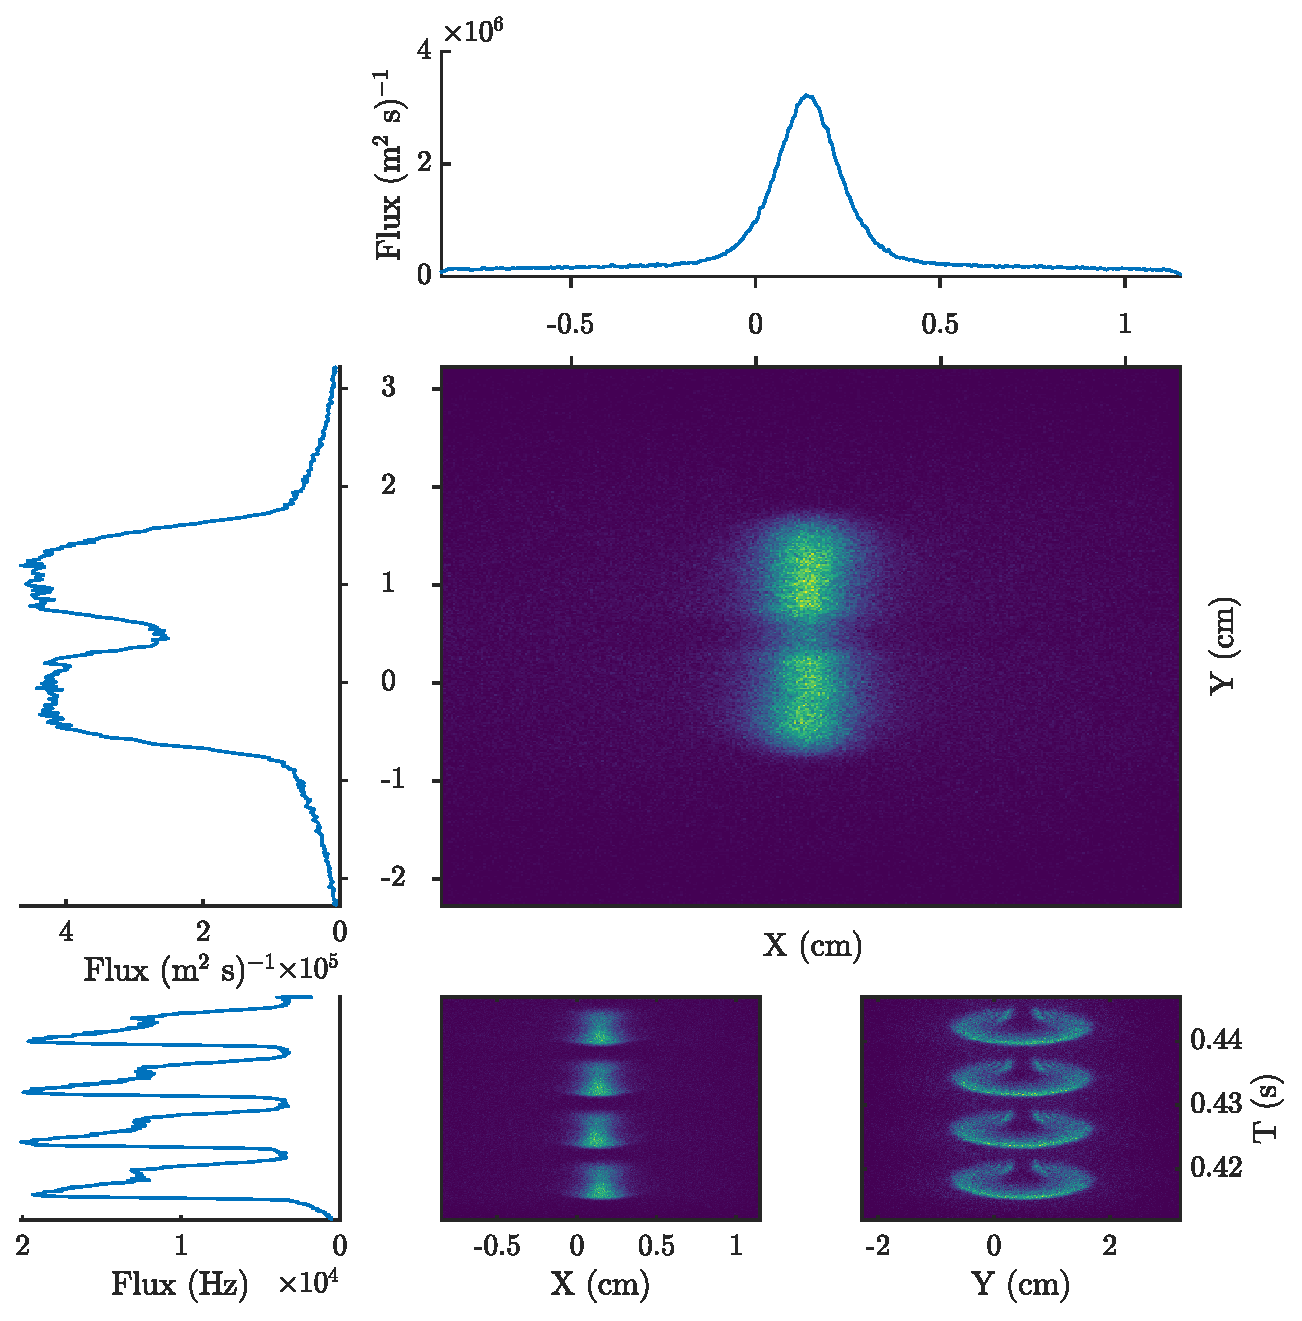
\includegraphics[width=\textwidth]{fig/apparatus/dropped_pal}
	 	\caption{MCP readout of the first few pulses from a pulsed atom laser, displayed similarly to Fig. \ref{fig:dropped_bec}. When atoms are transferred into the untrapped state, they are repelled from the trap by the mean-field energy of the remaining condensate, leading to pulse broadening especially in the tight $(y,z)$ axes. In the dilute outcoupled pulse, the speed of sound is low enough that the relative velocity of the pulse and BEC is supersonic in the outcoupled cloud, leading to the complex interference patterns which have been identified as \emph{Bogoliubov-Cerenkov radiation}\cite{Henson18_BCR}. The peak flux is about a thousandth of that for a dropped BEC, and hence saturation is avoided.
	 	% \footnote{This can be verified in two ways: One, for BECs of $N_0$ atoms, and variable outcoupling rate $\beta$ the pulse populations $N_i$ are proportional to the outcoupling rate. Two, within a single shot and fixed outcoupling rate $\beta$ the pulse populations decay geometrically, which would not be true were saturation evident in the earlier pulses.}. 
	 	The flat top of the Y-projection is due to the distortion of the profile during the trap escape, not detector saturation.}
	 	\label{fig:dropped_pal}
	 \end{figure}
	 \newpage

\subsection*{Atom lasers}
	\label{sec:atomlaser}


	% 	NB - the Einstein coefficients have a cubic dependence on frequency (See also the natural lifetime) and so optical transitions tend to exhibit spontaneous decay more quickly than the Rabi oscillations, but radio transitions (as in the fine structure states) fall much more slowly and coherent oscillations can be seen 
	% One can see that at large detunings, the oscillation frequency ncreases but the amplitude falls off like the detuning-squared, and one instead encounters the dipole potential, right?

	The most straightforward way to use an MCP-DLD to interrogate a BEC is simply to drop the atoms onto the detector.
	An example of this straightforward detection scheme is illustrated in Fig.
	\ref{fig:dropped_bec}.
	A drawback of this method is that the high atom fluxes in large BECs can temporarily deplete the available current carriers near the surface of the detector, resulting in a nonlinear reduction in detection efficiency known as \emph{saturation}.
	This means that for even moderately sized condensates, a determination of the condensate population by counting detection events or by straightforward fitting of the time-of-flight profile is impractical, and one cannot compute interesting quantities like correlation functions with meaningful accuracy.
	Another limitation of the trap-release method is that it is a completely destructive measurement - one cannot re-trap the cloud or only drop part of it, which slows down data acquisition for even simple purposes like determining the trapping frequencies.
	Atom lasers can circumvent both of these issues.
	

	The basic principle of an atom laser is to transfer some portion of the condensed atoms into a state that is no longer confined by the trapping potential.
	This was first achieved (shortly after the first realisation of BEC) by applying pulses of RF radiation to a magnetically trapped condensate \cite{Mewes97}.
	Later, a continuous-wave atom laser was demonstrated and used to perform RF spectroscopy of the cloud, revealing the symmetry-breaking action of gravity which pulls the BEC away from the minimum of the magnetic field \cite{Bloch99}.
	Optical Raman transitions\footnote{In atom optics, \emph{Bragg} transitions, which impart a momentum transfer, are distinguished from  \emph{Raman} transitions which induce a change in the electronic state.} can also be used as the outcoupling mechanism \cite{Hagley99} with the advantage of imparting a controllable momentum to the outcoupled atoms, but are not employed in the works in this thesis.
	

	Atom lasers are so named because the trapped condensate acts as a reservoir of coherent matter waves, in analogy to lasers as a source of coherent light \cite{Naraschewski99,Glauber63}.
	The first-order coherence of atom lasers is evident from the observation of interference fringes between matter-wave beams \cite{Andrews97} and the higher-order coherence manifests in the many-particle correlations detected in \mhe~atom lasers \cite{Manning10,Dall11a,Rugway11}.
	Atom lasers can also be collimated \cite{Bloch99}, directed with collimated laser beams playing the analogous role of an optical waveguide \cite{Guerin06,Couvert08}, and manipulated with optically-induced `mirrors' and beamsplitters \cite{Bloch01}.
	The potentially continuous operation of atom lasers \cite{Chikkatur02} brings the analogy with conventional lasers even closer.
	Atom laser physics has been studied in detail and widely deployed through the field of atom optics in the two intervening decades since their conception, including all of the experiments described in this thesis.
	
	% NB this Andrews paper makes some interesting points about the nature of the condensate order parameter, arrguments about whether BEC is actually coherent/hhas a phase, and the relationship between gauge symmetry breaking and particle number conservation - c.f.
	% that recent paper about number fluctuations in a condensate, discuss in overview


	A simple explanation of the mechanism of an atom laser requires a two-level atom with magnetically trapped and untrapped states labeled $\ket{1}$ and $\ket{0}$.
	An RF pulse tuned to the splitting $\omega_{10}$ induces an oscillation between the two states with Rabi frequency $\Omega$ for a duration $t$.
	For an ensemble of $N$ atoms, the independent single-particle oscillations produce a many-body product state which evolves as \cite{Mewes97}
	\begin{align}
		\ket{\Psi} &= (\cos(\Omega t/2)\ket{0} + \sin(\Omega t/2)\ket{1})^{\otimes N} \\
		& = \sum_{n=0}^{ N}\sqrt{\frac{N!}{n!(N-n)!}}\cos(\Omega t/2)^{N-n}\sin(\Omega t/2)^n\ket{N-n,n},
		\label{eqn:PAL_Rabi}
	\end{align}
	where $\ket{N-n,n}$ denotes the state with $n$ atoms coupled out of the trapped state and $N-n$ atoms remaining.
	The outcoupled fraction is then $\sin^2(\Omega t/2)$.
	% \footnote{There is the question of when the atoms actually leave the trap.
	% In one picture, the RF pulse simply allows the atomic wavefunction to couple periodically to the decay channel corresponding to collision with the detector.
	% So they don't actually 'leave' the trap until there's a detection event.}.

	In practise, the Zeeman splitting varies across the trap due to the inhomogeneous magnetic field, and so a narrow RF pulse would only be resonant with a section of the condensate.
	While useful for detailed spectroscopy of the condensate, the outcoupling rate would depend on the condensate population.
	This can be circumvented by applying short RF pulses resonant with the minimum Zeeman splitting of the trap.
	If such pulses are sufficiently short, the Fourier broadening of the finite-duration pulse is wider than the RF width of the condensate.
	The typical radio-frequency width of the condensate, i.e.
	the difference between the resonant frequency at the centre and the edge of the condensate, is set by the chemical potential of the condensate and is typically less than 10 kHz in our experiments.
	The outcoupling pulse typically consists of 6-10 cycles of RF tuned to the Zeman splitting of the trap bias, which typically ranges from 0.6-1 MHz depending on the configuration that is most suited to the experiment at hand. 
	This leads to pulses that range from about 5-25 $\mu$s, where the number of cycles is the most direct means to control the outcoupling rate (c.f. Eqn. \ref{eqn:PAL_Rabi}).
	An example of the MCP-DLD readout from a pulsed atom laser is shown in Figure \ref{fig:dropped_pal}.

	% Therefore, an RF pulse duration of order X sec is sufficient to ensure a uniform transfer across the trap.
	
	
	 % The pulses typically on the order of 100$\mu$s long, which for a typical trap splitting of order 2MHz ensures the spectrum of the pulse has a FWHM of order xMHz thanks to Fourier broadenin.
	


% PAL picture is integrated over 156 shots from 5_3d_2_3 data
% QD picture is integrated over about 1300? in tight trap fwiw from run 8

% PAL parameters; 1.6-3 MHz centering (see that ol plot) depending on trap
% pulsees 6-12 cycles
% typically sampled at 6-11 ms periods, generally limited by BEC width
% 




	


\section{Data acquisition \& control}
\label{sec:DAQ}
	
	Control of the optical components, coil current supplies, and RF radiation is coordinated by a central LabView program which transmits pulse sequences to the machine via National Instruments pulse generation cards.
	The cards themselves are connected to the CPU by a PCI bus, and synchronize their internal clocks at the beginning of each shot.
	The cards also record analog inputs such as Fabry-Perot cavity scan traces, photodiode traces, and mains voltage traces for post-processing diagnostics.
	The spectroscopic laser lock and tuning operations are also performed on the main control computer, as described in section \ref{sec:spec_laser}.

	The LabView control is supplemented by a command that calls a MATLAB subroutine (referred to as the `interface'), which is customizable to suit the purposes of a given experiment\footnote{The software developed to analyse the data from various experiments is invariably written in MATLAB.	Many core capabilities are stored in the repository \url{https://github.com/HeBECANU/Core_BEC_Analysis}, and generally each project will have a unique public repository as well.}.
	The motivation for this extension was for automatic and more flexible variation of experimental sequences. 
	This subroutine can return the \verb|.xml| file path of a LabView pulse sequence file for use in the next experimental cycle, and even modify the sequences, albeit in a limited way due to the particulars of LabView's sequence specification format.
	This extension allows for automatic optimization of experimental sequences, as was demonstrated in \cite{Henson18_ML}, but obviously is of no use for mechanical tasks like beam alignment\footnote{One can dream, though.}.
	Moreover, running back-to-back measurement and calibration shots would otherwise have to be done manually, as would updates of the spectroscopic laser wavelength during scans across the spectral region of interest.
	Therefore without the automatic update procedures enabled by the interface, the multi-day data collection runs embarked upon in this thesis would have become considerably more time-consuming and error-prone. 
	
	The interface script also writes metadata to a log file, including the POSIX timestamp, type of shot executed (e.g.
	\verb|calibration| or \verb|AtomLaser|), shot number, and other relevant parameters.
	The timestamps in this logfile can be cross-referenced with the \verb|txt| files that are written by the TDC computer and with the LabView logs of analog inputs in order to match the experimental parameters with data files for post-processing purposes.
	The data analysis pipelines for modern experiments can be complex, and the experiments in this thesis generally comprise a handful of different diagnostics processed in parallel.
	The tagging of shots by timestamp cross-referencing allows separation of relevant shots for each processing subroutine.
	
\subsection{Laser lock control protocol}

	As mentioned, the interface plays an important role in scanning the spectroscopic laser set point across regions of interest (be they electronic transitions as in chapter \ref{chap:transitions} or the tune-out wavelength in chapter \ref{chap:tuneout}). 
	The relationships between the subroutines involved in the laser control system are illustrated in Fig. \ref{fig:tcp_control}.
	The major features of this system architecture are two parallel processes which communicate with each other via MATLAB's cross-thread communication (\verb|labSend(data,to_process_id)| and \verb|labReceive(from_process_id)|).
	The messenger thread (T1) continuously looks for a TCPIP connection with the interface, which runs at the start of each experimental sequence and opens a TCPIP channel for the thread to connect with and receive the new setpoint.
	The control thread (T2) operates a PID loop by querying the wavemeter for its present reading (via USB connection) and also querying the laser control module for relevant parameters (particularly internal photodiode readings and voltages across piezoelectric actuators for interal optomechanics).
	The control loop then compares the desired set point to the measured set point and updates the actuator voltages according to the output of a discrete PID function.
	The control thread (T2) also contains a subroutine which is triggered when T1 sends the new setpoint through via \verb|labSend()| (which sets the \verb|labSend| bit to 1).
	If this condition is met, then T2 updates the setpoint for the PID loop with the new value obtained from \verb|interface| via T1.
	There is a stall condition here where the TCPIP port is opened by \verb|interface| but T1 is still waiting for the timeout of the last query, hence \verb|interface| will hang until the next loop of T1.
	This is not a major problem as the interface script must terminate before the pulse generation cards are triggered (they are sequential in the LabView program), so rather than interrupting the experimental execution it simply reduces the PID bandwidth briefly at the start of each run.
	The loop bandwidth is speed-limited by the frequent condition checks, device queries, MATLAB's limited speed as an interpreted language, and competition with other processes for CPU time. 
	Nonetheless the lock loop maintains a clock speed on the order of 10-15 Hz.
	The system has sufficient bandwidth to achieve a $\sim900$~ms rise time (10\% to 90\%) for a $\sim300$~MHz frequency step, and during interrogation we measured a typical (in-loop) standard deviation of 170~kHz. 
	The stabilization of the laser frequency uses measurements of the red side of the laser system (before the doubling cavity), so interruptions to the doubling cavity do not impact the lock.
	

	\begin{figure}
		\centering
		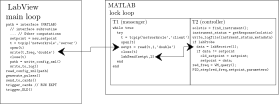
\includegraphics[width=\textwidth]{fig/apparatus/lock_loop}
		\caption{Schematic of the three major components of the lock loop used to scan the laser setpoint during spectroscopic measurements. As detailed in the main text, the main LabView script calls MATLAB subroutine which, among other tasks, communicates with a parallel pair of worker threads T1 and T2 which actuate the SolsTi:S controls.}
		\label{fig:tcp_control}
	\end{figure}




% tcpip interface for laser lock
% 	t = tcpip(IP, 33333, 'networkrole','server')
% 	fopen(t)
% 	fwrite(t,freq,'double')
% 	fclose(t)

% And on the other end - a loop that hammers it with queries?
% init parallel pool
% 	if workerID == 1
% 		while true
% 			try
% 				t = tcpip('localhost',33333,'networkrole','client')
% 				fopen(t)
% 				setpt = fread(t,1,'double')
% 				fclose(t)
% 				labSend(setpt,2)
% 			end
% 		end
% 	elseif workerID ==2 
% 		solstis = find_instrument();
% 		instrument_status = getResponse(solstis)

% 		write_logfile(instrment_status,metadata)
% 		% Omitting parameters for lock loop like wait times, slew rate limits, etc, various timers,

% 		if labProbe
% 			data = labReceive(1);
% 			if data != setpoint
% 				old_setpoint = setpoint;
% 				setpoint = data;
% 		red_freq = WM_query();
% 		PID_step(red_freq,setpoint,parameters)


% -> Something about communication between parallel workers?
% Ethernet link between PC and solstis driver; query returns machine state like internal photodiode readings and optomechanical actuator voltages


\subsection*{Optimizing machine performance}

	% Routine maintenance is required to keep the machine capable of producing large condensates.
	Despite the stabilized environment, optics are prone to wander slightly over time.
	The stable temperature is especially important as the cooling beams are coupled from the AOM tables to the vacuum chamber optics by free-space links.
	Drift in the relative position of the optics tables would therefore result in misalignment of many laser beams, and degrade performance of the machine.
	The conditioned air is supplied through three HEPA filters in the lab ceiling.
	The resulting positive pressure in an area enclosed by PVC strip walls keeps dust from entering the area on air currents.
	

	If the second MOT is loading and a saturated fluorescence signal is visible, one can usually optimize all of the optical alignments on this signal, which is a factor of ten faster than the full BEC creation sequence.
	If this is not available, logs of diagnostics taken at several points throughout the beamline can facilitate diagnosis of the point of failure.
	The most commonly employed tests are Faraday cups which produce a current when impacted by \mhe~atoms, as read out on a picoammeter.
	These current sensors are placed after the deflection stage, at the end of the Zeeman slower (with a large hole bored through it to allow the slowing beam to pass through), between the first MOT and the focus stage, and behind the second MOT chamber.
	In case the first MOT is not operational, a Xenics Bobcat CCD camera mounted above the chamber provides a view of the trapping region and direct visual feedback about the presence, shape, and density of the MOT.
	


	% A more elegant solution could take the form of a main script that generates control pulses, absorbs the functions of the interface while monitoring the TDC output directory, and creates a direct link between log files and the \verb|d.txt| files.
	% Unfortunately, even if LabView were able to provide all this functionality, upgrading the control software would be like moving deckchairs on the titanic.
	% It would be more effective to replace the entire control suite, which could take several months.
	% Given the long build times required for new experiments, during which continuous operability is essential, and that adjusting the control software is a relatively small part of the demands of operator time, this upgrade is not a high priority.
	%  However, the control software for Staggering Grace was recently upgraded to a more readily usable and modifiable Python-based infrastructure, which will surely prove both helpful and informative for future designs.

    % \begin{figure}
    % 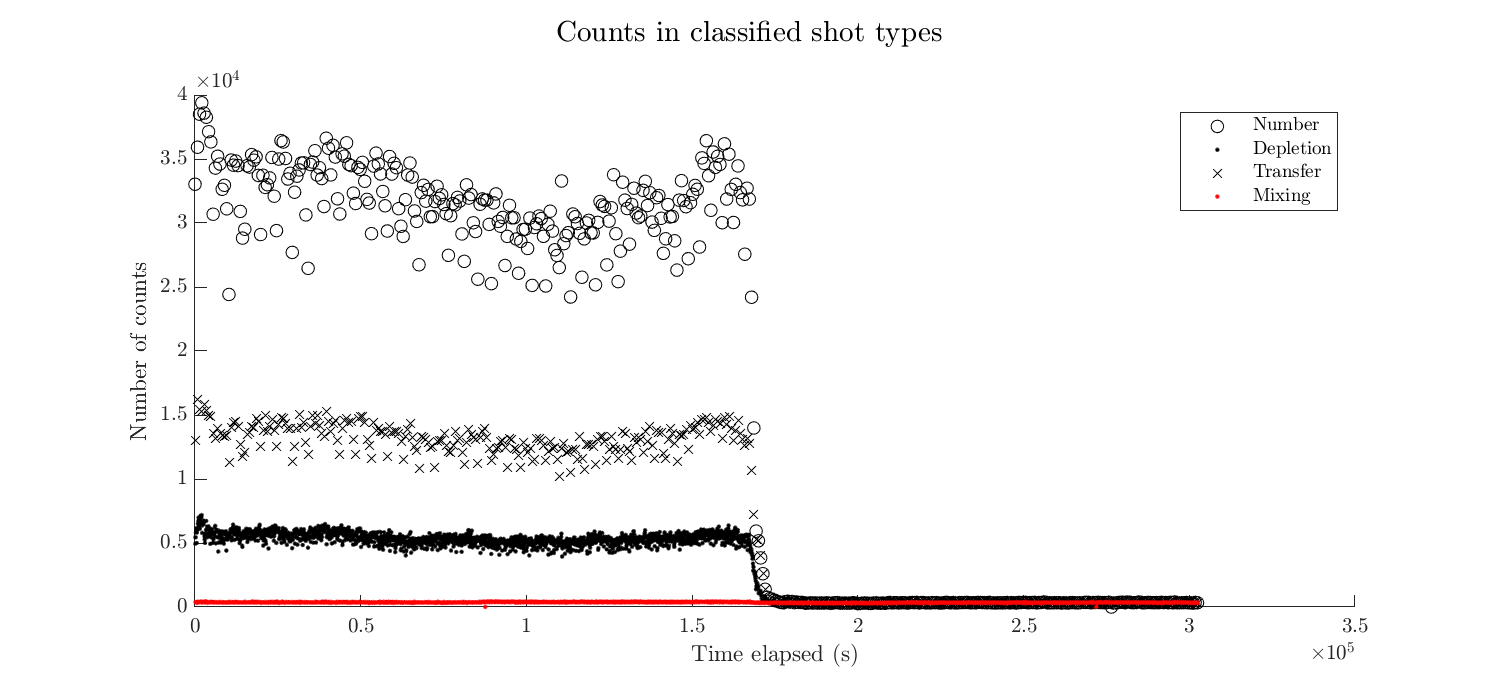
\includegraphics[width=\textwidth]{fig/depletion/partition_QD_files_01_shot_counts_combine}
    % \label{fig:qd-count_by_type}
    % \caption
    % \title
    % \end{figure}





   
 % %   Notes on new BEC paper
	% % We report the realisation of Bose-Einstein condensation (BEC) of metastable helium atoms using an in-vacuum coil magnetic trap and an optical dipole trap.
	% A novel quadrupole-Ioffe configuration (QUIC) magnetic trap made from in-vacuum hollow copper tubes provides fast switching times while generating traps with a 10G bias without compromising optical access.
	% The bias enables in-trap 1D doppler cooling to be used, which is the only cooling stage between the magneto-optic trap (MOT) and the optical dipole trap.
	% This allows direct transfer to the dipole trap without the need for any additional evaporative cooling in the magnetic trap.
	% The entire experimental sequence takes 3.5 seconds, with essentially pure BECs observed with ∼ 1e6 atoms after evaporative cooling in the crossed dipole trap.

	% % Get Herwig Ott paper [7] for thesis ref

	

	% % Can extract mu via R_tf ^2 / 2t_tof ^2, and so from TF picture get N_0 = (2mu)^{5/2}/(15\sqrt{m}\hbar\bar{\omega}^3 a).
	% % Cross T*_c at 6\mu K with 3e6 atoms, down to 80% BEC with 1e6 atoms


	% % is that supposed to be a dot product?.
	% The dipole potential is proportional to the intensity and the real part of the polz, which descrives the in-phase component of hte oscillation.
	% The force is given by the gradient of this potential.
	% The absorption from the driving field (and reimission in steady-state) is 
	% % $P_{abs} = \langle\dot{\textbf{p}}\textbf{E}\rangle = \frac{\omega}{\varepsilon_0 c}Im(\alpha) I$.
	% The scattering rate is therefore $P/\hbar\omega$.
	% The Lorentz oscillator considers an electron with an SHO-like elastic binding to a fixed nucleus, with natural freq $\omega_0$ and a damping rate $\Gamma$.
	% The resulting DE 
	% % $x''+\Gamma_{\omega}x'+\omega_0^2x = -e E(t)/m_e$ includes the natural decay rate 
	% % $\Gamma_{\omega} = e^2\omega^2/6\pi\varepsilon_0 m_e c^3$, which gives a solution for 
	% % $\alpha=\frac{e^2}{m_e}\frac{1}{\omega_0^2-\omega^2-i\omega\Gamma_\omega}$.
	

	% % In the limit of large detunings, negligible saturation, and in the rotating wave approx, one finds
	% % $$
	% % U_{dip}(r) = \frac{3\pi c^2}{2\omega_0^3}\frac{\Gamma}{\Delta}I(r),
	% % $$
	% % $$
	% % \Gamma_{sc} = \frac{3\pi c^2}{2\hbar\omega_0^3}\left(\frac{\Gamma}{\Delta}\right)^2I(r),
	% % $$
	% % Yielding the useful relation $\hbar\Gamma_{sc} = \Gamma U_{dip}/\Delta$, indicating two important principles: The scaling with intensity and detuning, and the importance of the sign of the detuning.

	% % In multilevel atoms, one can extend the argument to other higher-lying states and compute the polarizability farther from several resonances, which leads towards tuneout wavelenghts...


	% % This semiclassical model captures the absorption and stimulated emission of light from an electromagnetic field, but does not explain spontaneous emission.
	% A fully quantum-mechanical treatment of the system (such as the Jayne-Cummings model) will also fail in this respect.
	% The mechanism of spontaneous emission requires the theory of QED for a full explanation, wherein vacuum fluctuations produce short-lived virtual particles - including photons - which occasionally have the right wavelength to stimulate emission from atoms.
	% We will not explore this detail here, but remain satisfied with the natural lifetime 
	
	


	% % The interaction of an electric field with an atom induces a dipole $-e\textbf{r} - \varepsilon_0 \chi_a \textbf{E}$, where $\varepsilon_0\chi_a$ is the scalar polarizability (there are higher terms, as treated later).
	% The interaction energy is 
	% % $U=-\frac{1}{2}\varepsilon_0\chi_aE^2$ - by reference to the work above.
	% The force follows from $F = -\nabla U$.
	% A radiation field with frequency $z$ propagating along the $z$ direction gives rise to a force, averaged over timescales much larger than $1/\omega$, which can be written in terms of the Bloch components
	% % $$
	% % \bar{F}_z = \frac{-\hbar\Omega}{2 E_0}(u\frac{\partial E_0}{\partial z} - v k) = F_{dipole}+F){scatt},
	% % $$

	% % where $k$ is the wavenumber of the light, finally giving rise to 
	% % $$
	% % F_{scatt} = \hbar k\frac{\Gamma}{2}\frac{\Omega^2/2}{\delta^2+\Omega^2/2+\Gamma^2/4}
	% % $$

	% % $$
	% % F_{dipole} = -\frac{\hbar\delta}{2}\frac{\Omega^2}{\delta^2+\Omega^2/2+\Gamma^2/4}\frac{\partial\Omega}{\partial z},
	% % $$
	% % The latter goes to zero on resonance ($\delta=0$).
	% This argument applies for all three spatial dimensions and so one arrives at $U_{dipole} \approx \frac{\hbar^2\Omega}{4\delta}$, once again.
	% One can also arrive at a similar expression for the radiative force by considering a simple model of photons with wavenumber $k$ being absorbed and emitted at a rate $\Gamma$, where the re-emission process imparts a zero impulse on average, but is limited in temperature.
	% % from \cite{Grimm00}


	% % An experimentalist is occasionally required to negotiate the geometry of trapping fields, laser beams, and polarization vectors in order to correctly configure optics.
	% A method follows.

	% % For an electric field propagating with a wavevector $\vec{k}$ in the lab frame across an atom in a magnetic field $\vec{B}=B\hat{\vec{B}}$...
	% % 	The electric field of a purely polarized light ray at a point in space can be expressed as

	% % $$
	% % \textbf{E}(t)=\begin{bmatrix}
	% % E_x(t)\\
	% % E_y(t)\\
	% % E_z(t)
	% % \end{bmatrix}
	% % $$

	% % If we fix the axis of propagation to be $\hat{z}$, then we can write

	% % $$
	% % \textbf{E}(t)=\begin{bmatrix}
	% % E_{x0} e^{i(kz-\omega t -\phi_x)}\\
	% % E_{y0} e^{i(kz-\omega t -\phi_y)}\\
	% % 0
	% % \end{bmatrix}
	% % $$

	% % We can then define the Jones vector $\textbf{J}_0 = \left(E_{x0}e^{i\phi_x},E_{y0}e^{i\phi_y}\right)^T$, so $\textbf{E}(t) = \textbf{J}e^{i(kz-\omega t)}$.

	% % In this frame, the amplitudes of horizontal and  vertical polarization are $E_{x0}$ and $E_{y0}$ respectively.
	% Therefore, diagonal polarization is a linear combination of both these components, and circularly polarized light is a linear combination with an imaginary coefficient.
	
	% % A shortcoming of the Jones calculus is that it is only applicable to light which is completely polarized (that is, for some basis it can be written as $\textbf{E} = (E_0,0)$).
	% This is not true for a beam whose polarization varies, or where there are power fluctuations in one of the axes, etc.
	% There should be a single motivating example somewhere, but these are some examples.
	% If this assumption is not permitted - by which measurement would you tell the difference? - then we must move to the Mueller calculus.
	% %Determining purity of polz empirically


	% % When working with two-level systems it is convenient to introduce the density matrix $\rho$.
	% The assumption that the system must always be in \emph{some} state can be written as the normalization condition
	% % \begin{align}
	% % 	1&=\sum_i |\braket{\phi_i}{\psi}|^2\\
	% % 	 &= \sum_i \braket{\phi_i}{\psi}\braket{\psi}{\phi_1}\\
	% % 	 &= \textrm{Tr} \rho,
	% % \end{align}
	% % where the Trace operation is defined by $\textrm{Tr}(\ket{a}\bra{b})=\braket{b}{a}$.
	
	% % The density matrix permits a statistical approach to ensembles of conditional states, which will be useful in later chapters, and unifies the treatment of the important features of atom-light interactions, which is the subjects of the rest of this section.
	% \footnote{The density matrix formalism also allows for treatment of statistical mixtures of quantum states on equal footing with so-called `pure' states which are certain to be in some state $\ket{\psi}$.
	% While the normalization condition is guaranteed to hold for any $\rho = \sum_i p_i\hat{rho}_i$, there is no such way to write mixtures in the form $\ket{\Psi}=\sum_i\ket{\psi_i}$ without violating the assumption of conservation of probability.
	% Indeed, pure states, defined by $\textrm{Tr}(\rho^2)=1$, are quite exceptional: They are a set of zero measure in the set of all positive semidefinite Hermitian operators with unit trace.}.
	% When expressing the state  in terms of the energy eigenbasis $\{\ket{n}\}$, the diagonal elements $\rho_{ii}\in\mathbb{R}$ are the \emph{populations} of the $i^{\text{th}}$ eigenstate and the off-diagonal \emph{coherences} $\rho_{ij}=\rho_{ij}^{*}$ capture the utility of the quantum state for interferometric purposes\footnote{In what sense? c.f.
	% Ramsey interferometry}.
	

	% % By working in a rotating reference frame via the change of basis\footnote{This change of basis induces a change to the coefficients $c_n=\exp((-1)^n \delta t/2)$} $\hat{U} = \textrm{diag}(e^{i\delta t/2},e^{-i\delta t/2})$, in terms of the detuning $\delta=\omega-\omega_0$, one can write the Hamiltonian in the convenient form \cite{FootAtomic}

	% % \begin{equation}
	% % 	\hat{H} = \frac{\hbar}{2}\begin{pmatrix}\delta&\Omega\\
	% % 											\Omega&-\delta\end{pmatrix},
	% % \end{equation}
	% % which has eigenvalues $E'_\pm = \pm \sqrt{\delta^2+\Omega^2}/2$, retaining the bare splitting $\delta$ between levels when $\Omega=0$.
	% In the presence of an oscillating field which drives an allowed transition, i.e.
	% when $\Omega>0$, the energy of the \emph{dressed state} of the atom are shifted with respect to their unperturbed values

	% % %  For now we will simply note that the average of a set of measurements of the quantity $Q$ on an identically-prepared system can be calculated via the expectation value of the corresponding operator $\hat{Q}$,
	% % % \begin{align}
	% % % 	\langle Q\rangle &=  \bra{\psi} \hat{Q}\ket{\psi}\\
	% % % 	&= \textrm{Tr}(\hat{Q}\rho),
	% % % \end{align}
	% % % and that the time-dependence of the expected value follows from Ehrenfest's theorem
	% % % \begin{equation}
	% % % 	i\hbar \frac{\partial}{\partial t}\langle Q\rangle = [\hat{H},\hat{Q}],
	% % % \end{equation}
	% % % which holds equally well for the density matrix, providing the von Neumann equation $\dot{\rho} = i[\rho,\hat{H}]/\hbar$.
	
	% % Let us concern ourselves with a further simplified picture of the atom as well: Indeed, we model the atom with the simplest nontrivial quantum system, one with only two distinguishable states.
	% A two-level system permits convenient expression of the entire density matrix
	% % \begin{equation}
	% % 	\hat{rho} = \begin{pmatrix}
	% % 		\rho_{11}&\rho_{12}\\
	% % 		\rho_{21}&\rho_{22},
	% % 	\end{pmatrix}
	% % \end{equation}




	% % The wavefunction $\Psi$ of an electron of mass $m_e$ moving in a central potential $V(r)$ can be written in terms of the bound eigenfunctions (also called \emph{orbitals}) of the Schr\"{o}dinger equation
	% % \begin{equation}
	% % 	\left(\frac{-\hbar^2}{2m_e}\nabla^2 + V(r)\right)\psi_{nlm} = E_n\psi_{nlm},
	% % \end{equation}

	% % which have the form


	% % On the optical Bloch equations;
	% % Starting from the density matrix, 
	% % $$
	% % \begin{bmatrix}
	% % \rho_{11} & \rho_{12}\\
	% % \rho_{21} & \rho_{22}
	% % \end{bmatrix} = \ket{\Psi}\bra{\Psi},
	% % $$
	% % We make the unitary transformation into a rotating frame by $U=\exp(diag(-i\delta t/2,i\delta t/2))$, which is a gauge transformation such that the zero energy is exactly between the upper and lower states, 
	% % $\delta=\omega-\-\omega_0$.
	% This looks like a transformation $U = \exp(-i\sigma_z t)$ where $\sigma_z$ is the first of the Pauli matrices which generate the unitary group of dimension 2.
	% In the rotating frame one then has the Bloch vector defined by 
	% % $R_i = Tr(\rho\sigma_i)$.
	% One can then transform the differential equations for $c_i$ into the rotating basis and obtain the time evolution of the system which can be conveniently written in the form $\dot{R} = R\times W$ where $R$ is the Bloch vector and $W=\Omega\hat{e}_1+\delta\hat{e}_3$.
	 
	% % One can include damping by adding a decay term of the form $\dot{\rho}_{22} =-\Gamma\rho_{22} + \Omega \sigma_y/2$, which recovers the exponential decay of the excited state in the absence of a driving field.
	% We finally have the optical bloch equations, which (may) still be expressible in a neat vector form?
	% % $$
	% % \dot{u} = \delta v - \Gamma u/2\\
	% % \dot{v} = -\delta u + \Omega w - \Gamma v/2\\
	% % \dot{w} = -\Omega v - \Gamma(w-1)
	% % $$, 
	% % which capture the population dynamics of a two-level atom coupled to a radiation field near resonance with significant spontaneous decay.
	% A similar procedure can be extended to many-level atoms (one-two-many quote), and is employed in chapter X appendix Y to predict the SNR of interrogating the forbidden transition.

	% % In the rotating frame one can write the Schrodinger equation in terms of the amplitudes in the rotating frame 
	% % $$
	% % i\frac{d}{dt}(\tilde{c}_1,\tilde{c}_2) = \begin{bmatrix}\delta/2&\Omega/s\\\Omega/2&-\delta/2\end{bmatrix}(\tilde{c}_1,\tilde{c}_2),
	% % $$

	% % which has eigenvales $\lambda = \pm(\delta^2+\omega^2)^{1/2}/2$ - which reproduces the raw splitting $\delta$ in the absence of a field.
	% When $\Omega>0$ - see Cohen-Tannoudji for a deeper treatment of this dressed state picture.
	% When the detuning is much larger than the rabi frequency then one gets $\lambda\approx\pm(\delta/2 + \Omega^2/4\delta)$, which is the bare detuning with a light shift given by the second term.
	% The sign of the shift is given by the detuning.
	% This light shift, or AC stark shift, is what underpins the working of the dipole force.
	
	% % Dipole beams are widely used in biophysical contexts for manipulation of DNA, proteins, and even entire bacteria.
	% See Ashkin 1997 or Lang and Bloch 2003?
	% % $\varepsilon$
	
	% % Radiation pressure traps afew K deep, can cool to some 10s of $\mu$ K
	% % Typical dipole traps less than a mK deep!
	


	% % RGL Theory of AC stark shift for polz; [107-108] theory, latter Lorentz oscillator model, treats as SHO basically? Which is damped by emission of radiation - gives  second order ODE which can be solved.
	% Good for weak driving.
	
	% % Of course, corrections are needed when other transitions are important, i.e.
	% when fairly close to a strong line
	% % RGL [109] second order perturbation sums over all possible final states.
	
	% % % Sobel'man I, introduction to the theory of atomic spectral Pergamon press 1972
	% % show that the polzability can be written in the familiar alpha eqn 
	% % % A Derevianko, H katori, physics of optical lattice clocks, rev mod phys 83, 2011
	% % % J R P Angel, P G H sandars, the hyperfine structure STark effect, proc roy.
	% soc.
	% a, 305 1968		

\chapter{Towards an optical lattice trap for helium}
\markboth{\thechapter. TOWARDS A HELIUM LATTICE}{}
\label{chap:lattice}



	% \begin{adjustwidth}{1.5cm}{0cm}
	\begingroup
	\begin{flushright}
	
	\singlespacing{\fontsize{12}{12}\selectfont\emph{
	``It might be noted here, for the benefit of those interested in exact solutions, \\
	that there is an alternative formulation of the many-body problem:\\
	How many bodies are required before we have a problem? \\
	G.	E.	Brown points out that this can be answered by a look at history.	\\
	In eighteenth-century Newtonian mechanics,
	the three-body problem was insoluble.\\
	With the birth of general relativity and quantum electrodynamics in 1930,\\ 
	the two- and one-body problems became insoluble.
	And within modern\\
	quantum field theory, the problem of zero bodies (vacuum) is insoluble.\\
	So, if we are out after exact solutions, no bodies at all is already too many!"}\\
	- Richard Mattuck\footnote{R.
	Mattuck, \emph{A Guide to Feynman Diagrams in the Many-Body Problem}, Dover Books on Physics (1992)}
	}
	\end{flushright}
	\onehalfspacing
	\endgroup
	\vspace{1cm}

	% \end{adjustwidth}

\section{The many-body problem}


	In his 1972 essay \emph{More Is Different} \cite{Anderson72},  Philip W. Anderson argued that the constructionist hypothesis, that one can reconstruct the universe starting from known physical laws,  `breaks down when confronted with the twin difficulties of scale and complexity\footnote{Five years later, he was awarded the Nobel Prize in physics for his work on the electronics of magnetic and disordered systems}.' 
	In this he argues that composing a system out of many well-understood pieces with well-understood interactions will eventually give rise to  phenomena in need of `new laws, concepts, and generalizations'.
	Familiar examples in physics include quasiparticles and hydrodynamics, and even atoms, which compress enormous amounts of microscopic information into an effective description based on observed emergent regularities.
	Anderson acknowledges the utility of reductionism by noting that emergent features are always understandable in terms of their microscopic composition.

	A major challenge in science, then, is traversing this bridge between `macro' and `micro'.
	Simulations (on paper or \emph{in silico}) contribute to the `upward-pointing' inquiry which aims to explain emergent features in terms of elementary concepts.
	The rapid rise of computing power in the latter half of the twentieth century provided a boon to scientists by permitting direct interrogation of previously intractable theoretical models.
	Simulating systems can now be done en masse, in parallel, and with much less human effort than iterations of manufacturing, transporting, and characterizing physical samples.
	The design-build-test-learn cycle thus contracts, and humankind grows more proficient at the design of compounds or materials with desirable properties such as their light-harvesting efficiency or efficacy at neutralizing pathogens.
	In the quantum-mechanical context this project is particularly challenging because analytical models at the microscale may be conceivable but are often analytically intractable.
	
	Further, the amount of information required to describe a quantum state, and the computational effort needed to forecast its evolution, quickly become so large as to exhaust even the largest supercomputers.
	It was in 1982 that Richard P.	Feynman laid out a proposition for the now-burgeoning field of \emph{quantum simulation} \cite{Feynman82}:

	\bigskip

	\begin{flushright}
	\singlespacing
	\emph{The first question is, What kind of computer are we going to use to simulate physics? Computer theory has been developed to a point where it realizes that it doesn't make any difference; when you get to a universal computer, it doesn't matter how it's manufactured, how it's actually made. Therefore my question is, Can physics be simulated by a universal computer? ... the physical world is quantum mechanical, and therefore the proper problem is the simulation of quantum physics ... But the full description of quantum mechanics for a large system with R particles  has too many variables, it cannot be simulated with a normal computer with a number of elements proportional to R ... And therefore, the problem is, how can we simulate the quantum mechanics? There are two ways that we can go about it. We can give up on our rule about what the computer was, we can say: Let the computer itself be built of quantum mechanical elements which obey quantum mechanical laws.  ... Can you do it with a new kind of computer--a quantum computer? (I'll come back to the other branch in a moment.) Now it turns out, as far as I can tell, that you can simulate this with a quantum system, with quantum computer elements. It's not a Turing machine, but a machine of a different kind.}
	\end{flushright}
	\bigskip

	The hope, then, is that one can engineer \emph{quantum} systems that behave like a certain other, potentially hypothetical, system of interest and obtain useful data from it more efficiently than via conventional computing, when the cost is measured in some combination of time, energy, or some other convenient currency.
	One flourishing branch of this field of inquiry is the use of {optical lattices} to synthesize artificial crystals, scaled up some 10,000 times and many orders of magnitude colder than conventional solids.
	The ultracold atoms in such systems then play the role of electrons bound in the ion lattice of solid systems.
	Ultracold metastable helium offers an extension of the questions one can ask of optical lattice simulators by giving access to single-particle momentum information in three dimensions.
	This affordance opens lines of inquiry not accessible via low-resolution momentum measurements or particle position measurements, as discussed in the sections below.

	In this chapter I recount efforts towards constructing an optical lattice trap for helium.
	I will describe the motivation for the project and the basic model of interacting bosons which can tunnel between nearest-neighbour sites on a lattice, the Bose-Hubbard model.
	Then I will detail the stages of construction that were achieved, and give a short account of the progress that has been accomplished by other students in the meantime, resulting in the publication \cite{Abbas21}.
	
	

\subsection{There's always a bigger Hilbert space}


	Given two quantum systems $A$ and $B$ with $d_A$ and $d_B$ degrees of freedom each, the natural way to represent the composite of the two systems is the tensor product $\mathcal{H}_C$ of their respective Hilbert spaces $\mathcal{H}_A$ and $\mathcal{H}_B$ \cite{Carcassi21}, whose basis can be written as
	\begin{equation}
	\{\ket{e_C}\} = \{\ket{e_A e_B}=\ket{e_A}\otimes\ket{e_C}\}
	\end{equation}
	for all pairs $(\ket{e_A},\ket{e_B})$ of the basis vectors of $\mathcal{H}_A$ and $\mathcal{H}_B$, respectively.
	Thus the dimension of the composite system $d_C = |\{\ket{e_C}\}| = d_A d_B.$ A composite system of $N$ two-level systems provides a simple illustration of the resource challenge in that the total dimension of the Hilbert space is $2^N$.
	A pure state can be represented as a vector with $2^N-1$ coefficients (the asymptotically trivial reduction by 1 owing to the normalization of the wavefunction), but a general mixed state must be encoded in a density matrix while tracking $\mathcal{O}(2^{2N})$  coefficients.
	The Hamiltonian, if similarly stored as a full matrix, requires the full $\prod_i d_i\times\prod_i d_i$ matrix to be stored in memory (albeit typically with real-valued entries).
	If the complex coefficients are to be represented by pairs of floating-point numbers with single precision (for 8 bytes = 64 bits for the real and imaginary parts of each coefficient), the memory of a consumer-grade laptop is exhausted by the state vector of 16 two-level systems; the density matrix and Hamiltonian exceed available memory for even smaller systems.

	Fortunately, it is not always necessary to store the full Hamiltonian in memory.
	A sparse representation often suffices as most systems of interest exhibit local coupling only, and so most coupling constants are zero.
	However, matrix diagonalization algorithms exploit tradeoffs between memory use and compute depth.
	For instance, fully general matrix diagonalization executes in $\mathcal{O}(D^{3})$ time, where $D$ is the matrix dimension.
	Some specialized algorithms can perform faster (as low as $\mathcal{O}(D^{2})$) but this is still unfavourable when dealing with exponentially-growing matrices.
	Thus storing sparse matrices may save on memory but slows down the diagonalization.

	In the case of the physical state, physical insight can lead to reformulations of the problem in (potentially many) fewer dimensions, such as by identification of a few relevant degrees of freedom, symmetries in the system wavefunction, or by finding conserved quantities.
	In this respect we are sometimes limited by our own ingenuity, but in general we are limited by the need to include higher-order correlations when many-body degrees of freedom cannot be integrated out in a mean-field or Hartree-type approach.
	In these situations, the memory requirements for the state vector can  be reduced for purposes of simulations by using inventive representations.
	A full review of numerical techniques is far beyond the scope of this thesis, but we will note that exact diagonalization \cite{Zhang10} is complemented by an expanding suite of compression techniques including matrix product states \cite{Schollwock11} employing the iterative density-matrix renormalization group  method \cite{Dechiara08}, the multiscale entanglement renormalization ansatz \cite{Evenbly15}, quantum Monte Carlo simulations \cite{BeccaQMC}, and emerging techniques using artificial neural network representations of many-body states \cite{Carleo17}.

	Quantum-native platforms offer a route by which to circumvent some of these issues; clearly Nature has no trouble evolving the state of some $\mathcal{O}(10^{23})$ nuclear spins in solid materials (let alone all their electronic states).
	If one encodes the physics of interest \emph{directly} into another quantum system, then the space (memory) requirements of simulating quantum systems is obviated.
	This does present another challenge, which is the means of initialising the state, implementing time evolution, and obtaining accurate readout.
	A broad pallette of methods exists for quantum simulation with digital quantum computers, including Trotterization, linear combinations of unitary operators, qubitization (these and other methods are compared in \cite{Low19}).

	Important milestones have been reached along the way in trapped ions \cite{Hempel18}, quantum dots \cite{Hensgens17}, microcavity polaritons \cite{Boulier20}, and superconducting circuits \cite{Wilkinson20}, 
	while cavity QED \cite{Zhu18}, and photonic circuits \cite{Arrazola21} are also promising platforms for quantum simulation.
	A comprehensive review of the conceptual background and platforms and problems of interest (as of 2014) can be found in \cite{Georgescu14}.
	As of the time of writing this dissertation, the largest digital quantum computers have around 50 qubits, and are not able to implement fault tolerant quantum computation at a physically meaningful scale.
	While early claims to quantum advantage have made it to press \cite{Arute19}, so far these results relate to algorithms which do not correspond to any class of familiar physical systems, or even any otherwise-useful calculation.
	It is worth noting that this observation may well be out of date in half a decade given the rapid progress in quantum engineering.


	An important counterpart to universal digital quantum simulation is \emph{analogue} simulation.
	The closest analogy in conventional `classical' computing is the application-specific integrated circuit (ASIC).
	These present-day systems that are optimized to perform specific tasks much more efficiently than a general microprocessor built within the Von Neumann architectural paradigm, but might not be Turing-complete.
	Similarly, analogue simulators are direct and dedicated simulations of a specified family of Hamiltonians for exploration of that system in particular.
	The focus of this chapter is one particular platform for quantum simulation: Ultracold neutral atoms trapped in an optical lattice. 
	While schemes have been proposed for universal quantum computing with neutral atoms in optical lattices \cite{Brennen99,Henriet20}, this potential is still some way off \cite{Markov00}.
	Meanwhile, analogue simulation in optical lattices is flourishing.
	For the second time, we will note that `any attempt to produce a comprehensive review is out of date by the time it is published' and, in the below, survey some pivotal results in order to clarify the specific contributions that metastable helium atoms could make to the suite of capabilities in optical lattices.



\section{Quantum simulation with optical lattices}


	The groundbreaking experiment in quantum simulation with optical lattices was the achievement of the Mott insulating state \footnote{A hallmark of the Mott insulator is the suppression of number fluctuations at each lattice site (i.e.
	\emph{number squeezing}), which was first observed a year prior in \cite{Orzel01}.
	However, the later result was the first to completely eliminate site occupancy fluctuations in 3D - see \cite{Morsch06} for discussion.} in a lattice filled with ultracold bosonic atoms \cite{Greiner01}, realizing the proposition by Dieter Jaksch \emph{et al.} from three years prior \cite{Jaksch98}.
	The subsequent few years saw an explosion of foundational research and technical development, summarized in the reviews \cite{Morsch06,Bloch08}. 
	The following decade heralded many major advances in quantum simulation \cite{Bloch12,Gross17}.
	Theoretical foundations of the myriad models realized in lattices, and their context in a more general condensed-matter setting, are discussed in Refs. \cite{LewensteinLattices, Lewenstein07}.

	The central principle of an optical lattice is the careful deployment of the optical dipole force \cite{Grimm00} to synthesize a potential energy landscape with a persistent periodic structure.
	In simpler lattice configurations (as considered in this chapter), a stable laser is reflected back on itself, thus creating a standing wave so atoms in this optical field are subject to a periodic potential along the axis of propagation of the laser.
	Lasers which are red-detuned relative to the nearest transition and have a Gaussian profile provide an overall, approximately harmonic, confinement, but this is typically negligible over the scale of the occupied lattice.
	
	Additional laser beams can break the radial symmetry and induce two- or three-dimensional periodic structures.
	The simplest of these is a square lattice, but different optical arrangements can be used to generate more complicated geometries such as the hexagonal honeycomb \cite{Jotzu14},  triangular \cite{Becker10}, and Kagome lattices \cite{Jo12}, and the recently-emerging quasicrystal lattices \cite{Viebahn19}.
	The translational symmetry can be intentionally broken by superposing the speckle pattern of another laser \cite{Pasienski10} or by collinear propagation of another laser whose wavelength is close to an irrational multiple of the main lattice \cite{Rispoli19}.
	More generally, arbitrary potentials can be generated in up to two dimensions using a digital mirror device (DMD) in the Fourier plane to synthesize user-defined intensity patterns in the plane of the lattice \cite{Gross17}.
	
	
	An ever-expanding suite of additional techniques allow the experimentalist to furnish their lattices with sophisticated control over the dynamics.
	One can realize paradigmatic condensed-matter models including the Bose \cite{Greiner01,Miranda15,Rispoli19,Sherson10,Preiss15a} and Fermi \cite{Bakr09,Cheuk15,Haller15,Chiu18} variants of Hubbard models, their disordered cousin the Aubry-Andre \cite{Rispoli19} model, and Ising models \cite{Simon11}.
	Within these models, characteristic phenomena like higher-order tunnelling \cite{Folling07} and particle-hole pair formation \cite{Endres11} have been observed in optical lattices.
	The controllability of these machines has permitted extensive exploration of the phase diagrams of these models.
	Through varying parameters such as the ratio of the tunnelling and interaction energies (the latter often achieved via Feshbach resonances \cite{Chin10}), optical lattice experiments can explore the phase diagram of a range of systems \cite{Greiner01,Eckardt05,Jordens08,Jo09,Haller10,Simon11,Baumann10,Leonard17,Landig16,SachdevQPT,Endres12,Anquez16,Clark16}.
	Whereas a classical phase transition is associated with a non-analytic free energy at some boundary in the space of state variables, a quantum phase transition occurs at non-analytic points of the ground state energy of a combination of Hamiltonians $H = H_0 + g H_1$, where $g$ is some real coefficient \cite{SachdevQPT}.
	If $H_0$ and $H_1$ commute, then the eigenstates are common but varying the coupling leads to a level-crossing at some critical value $g_c$, either side of which the ground state has markedly different character (more generally the system will exhibit an avoided crossing, but the definition holds in either case \cite{SachdevQPT}).
	
	Quantum phase transitions have been central objects of study with lattice simulators \cite{Greiner01,Eckardt05,Jordens08,Baumann10,Endres12,Haller10,Leonard17,Landig16,SachdevQPT}.
	Over the preceding decade there has been much activity investigating \emph{topological} phase transitions, which are associated with a nonlocal order parameter capturing the long-range entanglement structure inherent in different topological phases \cite{Goldman16,Nakagawa14}.
	Condensed matter models featuring this kind of transition in optical lattices include Hofstadter models\cite{Aidelsburger13,Tai17,Miyake13} and the Haldane model \cite{Jotzu14}.
	These models are synthesized by applying additional optical fields to create lattices with complex tunneling terms, imbuing particle motion with a path-dependent Aharonov-Bohm phase \cite{Aidelsburger11,Aidelsburger13,Miyake13}.
	This permits creation of systems wherein neutral atoms can be made to follow the equations of motion of charged particles under the influence of electromagnetic fields \cite{Aidelsburger13,Tai17,Endres11,Rispoli19,Jo09,Simon11,Miyake13,Folling07,Jotzu14}.
	The transition between regimes of time-evolution characterized by distinct scaling laws, called \emph{dynamical} phase transitions between, can also be produced in lattices \cite{Clark16}, including dynamical topological transitions \cite{Nakagawa14}.
	On the other end of the energy scale, efforts are ongoing to extend the reach of the cold-atom lab to simulations of high-energy phenomena like matter coupled to non-abelian gauge fields \cite{Zohar16,Schweizer19,Tagliacozzo13} and the Schwinger effect of particle-antiparticle pair production \cite{Pineiro19}.	
	

\subsubsection{Frontier experiments with optical lattices}
	Another fascinating branch of inquiry led by optical lattice labs lies at the intersection of quantum information theory and the foundational questions regarding decoherence, the emergence of entropy in thermodynamics from unitary evolution, and the resulting familiar phenomena of classical states \cite{Osborne02,Osterloh02,Isakov11,Jiang12,Dalessio16,Goold16,Srednicki94,Amico08,Eisert15}.
	A modern picture entails that so-called eigenstate thermalization gives rise to classical thermodynamics even in unitary evolution \cite{Srednicki94,Dalessio16,Goold16}.
	The connection with quantum information is principally that sub-components of the system become entangled with one another as the system evolves, `scrambling' information about the inital configuration in non-local correlations.
	More specifically, although the global state remains pure (with nearly zero entropy) during isolated evolution, information exchange between subsystems entangles them.
	When performing local measurements, then, one discovers that the entropy of subsystems increases despite the whole system undergoing unitary evolution from an initially pure state.
	Sophisticated interferometric techniques have been implemented to measure the degree of entanglement between sites \cite{Brydges19,Daley12,Mouraalves04,Palmer05}.
	They then exhibit nonzero quantum \emph{mutual information} which is the difference between the entropy of the subsystems and the entropy of the entire system.
	The sub-additivity of the von Neumann entropy is a hallmark of the regime of quantum thermodynamics, whereas classical entropy is strictly additive.
	
	Optical lattice experiments are beginning to resolve relevant phenomena such as the growth of entanglement between subsystems coincident with the onset of thermalization \cite{Clos16,Kaufman16}.
	This work is enabled by several schemes for the measurement of entanglement in cold-atom systems \cite{Chiu18,Brydges19,Daley12,Mouraalves04}.
	The application of disordered and quasi-random lattices has permitted direct inquiry into wavefunction localization \cite{Anderson58,Dalessio16,Goold16,Srednicki94,Clos16,Kaufman16,Nandkishore15}, wherein the presence of disorder prevents the system from thermalizing and instead retains local information about its initial state over long timescales.
	As local order parameters are not obviously applicable to quantum hall states or spin liquids \cite{Isakov11}, which feature topological phases that are not locally distinguishable, non-local order parameters based on entanglement measures can distinguish between these collective states \cite{Isakov11,Jiang12}.
	Long-range entanglement also manifests in quantum phase transitions \cite{Osborne02} and shows scaling behaviour analogous to correlation functions at classical phase transitions \cite{Osterloh02}.
	Diatomic molecules also feature in lattices, contributing to cold chemistry \cite{Balakrishnan16} through studies of basic mechanisms like dipolar spin exchange \cite{Yan13}, enhanced interactions via Feshbach resonance \cite{Yang19} or microwave-dressed resonant interactions \cite{Yan20}.
	In fact, some schemes have been proposed for universal computation with dipolar molecules in optical lattices \cite{Yelin06, Micheli06}.
	% https://journals.aps.org/rmp/abstract/10.1103/RevModPhys.91.021001
	
\subsection{Quantum state microscopy}

	A key enabler of the studies described above are the techniques of quantum gas microscopy \cite{Bakr09,Cheuk15,Endres11,Haller15,Miranda15,Parsons15,Rispoli19,Sherson10,Miranda17,Preiss15a} which include state preparation and measurements of spin and on-site particle parity (and recently even population up to $N=4$ \cite{Preiss15a}), each with single-site resolution.
	Direct access to microscopic information renders density correlations readily measurable \cite{Endres11,Rispoli19}.
	Correlation functions are central in quantum field theory and quantify the probability distribution of joint measurements of many-particle operators $\mathcal{O}_i(x_i)$ at some coordinates $x_i$, generally taking the form
	\begin{equation}
		G^{(N)}(\textbf{x}) = \langle \prod_{i=1}^{N}\mathcal{O}_i(x_i)\rangle = \textrm{Tr}\left(\prod_i\mathcal{O}_i(x_i) \rho\right).
	\end{equation}
	Such correlation functions characterize the many-body nature of interacting systems through the Wick decomposition \cite{Wick50}.
	This theoretical result guarantees that when pairs of degrees of freedom do not interact, their correlation functions for all $N>2$ are expressible in sums of products of correlation functions with $N\leq2$.
	Thus observing a factorization (or not) of many-particle correlation functions of order $M$ into lower-order correlations serves to indicate the absence (or presence) of relevant interactions of more than $M$ degrees of freedom \cite{Schweigler17}.
	One implication is that experimental results can constrain the number of required terms in controlled approximation methods like cluster expansion or basis truncation techniques \cite{Hodgman17}.
	Another is that collecting correlation functions can effectively provide an operational solution to the many-body problem in that all relevant quantities of interest (higher-order correlation functions) can be inferred \cite{Schweigler17,Hodgman17}.

	Going a step further and predicting products of arbitrary observables would require determination of the many-body density matrix $\rho$.
	The process of determining $\rho$ is also called quantum state tomography because the density matrix contains non-local information but is only amenable to local projective measurements.
	Some platforms for quantum computation (such as superconducting qubits and photonic systems) are furnished with the ability to perform arbitrary unitary operations. 
	This capacity, coupled with the fast cycle time of such systems, makes it possible to perform exhaustive tomography of the density matrix for modestly-sized systems.
	For an atomic system containing tens of thousands to millions of atoms, using machines which operate over several seconds rather than microseconds, such a task is clearly not feasible - even leaving aside the computational resource demands.
	Therefore, correlation functions between the degrees of freedom of interest remain important tools of inquiry into the many-body dynamics of ultracold gases.
	
	An immediate caveat is that one is limited in the extent to which one can infer correlations between degrees of freedom other than those one has measured to obtain the lower-order correlations. 
	This presents an obstacle to obtaining certain interesting quantities from analogue simulators equipped with quantum gas microscopes.
	For instance, in particle physics a common exercise is computing the expected momentum correlations between the product particles after collision in accelerators, which is not readily achievable using the gauge-field simulators described above.
	On the other hand, condensed-matter physicists tend to study correlation functions for \emph{collective} degrees of freedom, a pertinent example being Bogoliubov modes (or phonons in general) which are not generally detectable by means of spatial correlations, and manifest in the correlated momenta of many particles.

	One aspect which has been hitherto underrepresented in the cold atom toolbox is \emph{momentum microscopy} \cite{Ott16}.
	As noted in \cite{Bergschneider18}, `many important aspects of quantum states are not accessible by position-space imaging alone: properties such as long-range coherence, currents and phase fluctuations are related to off-diagonal order, or coherences, in the many-body states.'
	Momentum correlations provide access to information about these many-body coherences through Glauber's foundational work in quantum optics \cite{Glauber63,Naraschewski99}.
	Optical lattice experiments have, to date, typically employed coarse measurements of momentum-space information, for instance by absorption imaging in the far-field.
	This provides estimates of the momentum density, which has been used to verify the Bogoliubov picture of phonon formation \cite{Vogels02}, to verify coherence of a Mott-insulating state through noise correlations \cite{Folling05}, and to obtain the second-order momentum correlation function for a 1D Bose gas \cite{Fang16}, but does not resolve single-particle information or higher-order correlations.
	
	\noindent As discussed in the introduction, metastable helium has previously been used to probe the coherence of degenerate quantum gases by measuring high-order momentum correlations (see the introduction to chapter \ref{chap:apparatus} and references therein).
	In particular, data from the BiQUIC machine at ANU was used to show that the three-particle correlations in ultracold scattering halos can be expressed in terms of two-particle correlations \cite{Hodgman17}.	
	Some promising methods for momentum microscopy with other elements have also been developed. 
	Most recently, fluorescence imaging of $^6$Li with a high numerical aperture objective has been used to measure the position and, separately, momentum of up to three atoms  \cite{Bergschneider18}. 
	While this method is currently limited to small numbers of atoms in one dimension, another advance \cite{Bucker09} can image the far-field momentum of some tens of thousands of atoms.
	The latter method uses a single-photon sensitive camera to detect atoms as they fall through a 2D sheet of resonant light, thus projecting out the momentum information in the vertical direction. 
	While this could be employed in a stroboscopic manner to obtain 3D information, this could require many experimental cycles, unlike \mhe~experiments with an MCP-DLD stack which intrinsically provide three-dimensional momentum information.
	Therefore while the new optical methods will surely bear worthy fruit, \mhe~experiments currently stand as the most effective way to perform three-dimensional momentum microscopy.
	

	



	

\subsection{The Bose-Hubbard model}

	One of the most accessible many-body systems to realize with ultracold bosons in an optical lattice is the Bose-Hubbard model.
	The Hubbard model was originally introduced to study the transition metals in an attempt to understand their magnetic properties \cite{SachdevQPT}.
	The Bose-Hubbard (or `boson Hubbard') model replaces the spin-1/2 fermions with spinless bosons, which might represent Cooper pairs of electrons in a superconductor tunnelling between superconducting regions - or bosonic atoms hopping between sites in an optical lattice.
	The proposal to realize this model in optical lattices was put forward by Dieter Jaksch \emph{et al.} in 1998 \cite{Jaksch98}.
	The Hamiltonian of this model is 
	\begin{equation}
		\hat{H}_B = -J\sum_{\langle i j\rangle}\left(\cre{a}_i\anh{a}_j+\cre{a}_j\anh{a}_i\right) 
		+	\sum_{i} \frac{U}{2}\hat{n}_{i}(\hat{n}_{i}-1) 
		- \mu\sum_{i} \hat{n}_i
		\label{eqn:BH_ham}
	\end{equation}
	where $n_i = \cre{a}_i\anh{a}_i$ is the particle number operator, $\mu$ is the on-site chemical potential, $U$ is the interaction strength, and $J$ is the tunneling energy.
	The interaction energy $U$ and $J$ are generally evaluated numerically  based on the respective integral expressions.
	The interaction energy is
	\begin{equation}
		U = \frac{4\pi\hbar^2 a}{m}\int |w(\vec{x})|^4~d^3 x,
	\end{equation}
	where $w(\vec{x})$ is the Wannier function \cite{Wannier37,Marzari00} representing the wavefunction of a particle localized at a single site.
	By approximating the potential minimum as a harmonic oscillator with trapping frequencies $\omega_i = \sqrt{4 V_j}/\hbar$, where $V_j$ is the depth of the $j^{\textrm{th}}$ beam, one can arrive at the approximate expression 
	\begin{equation}
		U \approx \frac{\hbar \bar{\omega}a_s}{\bar{a}_{HO}\sqrt{2\pi}}
	\end{equation}
	where $a_0$ is the scattering length, $a_{HO}$ is the size of the ground state wavefunction, and the overbars indicate the geometric mean of the respective quantities	\cite{Jaksch98}.
	The tunneling rate is given in general by
	\begin{equation}
		J_{i,j} = \int w(\vec{x}_i) \left(-\frac{\hbar^2}{2m}\nabla^2 + V_0(x)\right)w(\vec{x}_j)~d^3 x,
	\end{equation}
	which in the deep-lattice limit is approximately \cite{Jaksch98}
	\begin{equation}
		J \approx \frac{4}{\sqrt{\pi}} E_r\Big(\frac{V_0}{E_r}\Big)^{3/4}e^{-2\sqrt{V_0/E_r}},
	\end{equation}
	where $E_r = \hbar^2k^2/2m$ is the recoil energy of a single photon from the lattice beams.
	The simplest model to consider is one where only nearest-neighbour hops are possible, but in a homogenous (infinite) system one has $J_{i,j} = J(|i-j|)$ and this is not an onerous addition.
	The second-order tunnelling between next-nearest neighbours is much smaller than the tunnelling between nearest neighbours, but nonetheless has been observed in quantum gas microscopes \cite{Folling07}.
	
	The optical lattice realization of this model relies on the optical dipole force \cite{Grimm00}, whereby two counterpropagating lasers (in each dimension) create a standing wave pattern\footnote{The upgrade at ANU includes a design to reflect the lattice beams back on themelves, similarly to the MOT trapping beams.}.
	If the laser has wavelength $\lambda$, then the electric field creates a lattice with twice the spatial frequency (half the wavelength) $k_L = 2k_\lambda = 4\pi/\lambda$.
	In a lattice formed by a collimated, retro-reflected Gaussian beam, the time-averaged electric field gives rise to an optical potential that can be approximated by
	\begin{equation}
		V_0(\vec{x}) = - V_{L} e^{-2\frac{{\vec{r_i}}^2}{{w_i}^2}} \sin^2(k x_i)
	\end{equation}
	where the trap depth is given by the optical dipole potential of a two-level system,
	\begin{equation}
		V_{L} = \frac{3\pi c^2}{2{\omega_0}^3}\frac{\Gamma}{\delta}\frac{2P}{\pi {w_0}^2},
	\end{equation}
	and the exponential envelope is inherited from the Gaussian profile of the laser.
	
	In the case of a focused laser, there will be an additional longitudinal envelope due to the divergence of the beam.
	In a 3D lattice created by mutually orthogonal beams of equal power, and considering only the sites closest to the centre of the trap, the potential can be approximated by 
	\begin{equation}
		V_0(\vec{x}) = -\sum_{i=1}^3\Big( V_{L} \sin^2(k x_i) + \frac{m}{2}(\omega_i x_i)^2\Big)
	\end{equation}
	where the Gaussian profile is predominantly governed by the first ($x^2$) term in its Taylor series with small-amplitude trapping frequencies $\omega_i$.	
	For very cold gases, only sites near the centre of the lattice will be occupied, and the potential can be well approximated by retaining only the first term and considering the lattice to be uniform.

	The Bose-Hubbard model exhibits a quantum phase transition between superfluid and Mott insulating states at the point $U/zJ \approx 5.8$ where $z=2d$ is the number of nearest neighbours \cite{Jaksch98}.
	For a system of N particles on M lattice sites (with $N = nM$), the  Mott-insulating ground state has the form of a product of Fock states
	\begin{equation}
		\ket{\Psi_{MI}} \propto \prod_{i=1}^M (\cre{a}_i)^n\ket{0_i},
	\end{equation}
	which exhibits vanishing number fluctuations between sites \cite{Greiner01}.	
	In the regime where tunnelling dominates (at $U\rightarrow 0$) the ground state takes the form
	\begin{equation}
		\ket{\Psi_{SF}} \propto \left(\sum \cre{a}_i\right)^N\ket{0_i}
	\end{equation}
	which is a product of (local) coherent states with Poissonian statistics \cite{Greiner01}.
	
	The momentum representation of the Bose-Hubbard model can be obtained by the Fourier transform \cite{Zhang10} of the bosonic creation operators,
	\begin{equation}
		\cre{b}_q = \frac{1}{\sqrt{M}}\sum_{j=1}^{M}e^{i(2\pi q j/M)}\cre{a}_j
	\end{equation}
	in terms of which the Hamiltonian is
	\begin{equation}
		\hat{H} = -2J\sum_{q=0}^{M-1}\cos\left(\frac{2\pi q}{M}\right)\cre{b}_q\anh{b}_q + \frac{U}{2M}\sum_{q_1,q_2=0}^{M-1}\sum_{q_3,q_4=0}^{M-1}\cre{b}_{q_1}\cre{b}_{q_2}\anh{b}_{q_3}\anh{b}_{q_4}\delta_{q_1+q_2,q_3+q_4}.
	\end{equation}
	The latter sum represents momentum-conserving collisions and commutes with the total momentum $K = \sum_{q=0}^{M-1}(2\pi q/M)n_q$.
	For a one-dimensional system with $N$ atoms and size $M$, the system has dimensionality $D = (N+M-1)!/(N!(M-1)!)$ which rapidly outstrips the storage space of consumer-grade computers.
	The problem can be made much more tractable by neglecting interactions, as Ramakumar \emph{et al.} did in an exact diagonalization study of non-interacting bosons (in a combined lattice and overall harmonic confinement) for up to $N=M=1000$ in one dimension and 2500 bosons in a $50\times50\times50$ lattice \cite{Ramakumar07}.
	The state-of-the-art quantum Monte Carlo calculations currently find good agreement with experiments \cite{Cayla18,Herce21}.


	Later in this course of study, an optical lattice was loaded with \mhe~by the group at Institut d'Optique in Paris \cite{Cayla18}, which therefter achieved the Mott insulator transition \cite{Carcy19} and showed the critical behaviour at the transition boundary conformed with the three-dimensional XY universality class \cite{Herce21}.
	There remain many interesting topics of study\footnote{Besides, it will be important to obtain independent reproduction of surprising discoveries.}, and potential future pathways are discussed at the end of this chapter.

\section{Infrastructure upgrade}


	In this section we deal with the (literal) nuts and bolts of assembling a cold-atom machine.
	The obvious route toward a helium-filled lattice would be to upgrade the BiQUIC machine.
	The biggest obstacle on this route is the limited optical access to the chamber.
	For one, the windows are relatively small and so the beams would need to be inserted parallel to existing beams.
	In principle one could install flipper mirrors and switch in the MOT beams for the loading sequence and insert the lattice beams along fixed, stable optics.
	However, if the laser generation table could be described as a `forest of optics', then the space surrounding the BiQUIC chamber is a veritable jungle.
	In short, it is certainly plausible that the machine \emph{could} host an upgrade, but it would decommission the machine for some time.
	It is much more convenient to instead blow the dust off another machine lying dormant in the laboratory one floor above level 0 \footnote{The BiQUIC lab is the sole room at the sub-basement level of the school.}.

	Before my arrival in the lab, Dr. Hodgman (the PI of the project) and some students had put in good early miles refurbishing the discharge source and pumping the existing chamber down to around $10^{-10}$ Torr.
	Some of the cooling and trapping beams were present but most of the AOM suite was yet to exist.
	The prior incarnation of the machine consisted of a source chamber and a Zeeman slower terminating at a MOT chamber, and a secondary science chamber.
	The pre-existing chamber only had ports that were small enough to clip the first-order diffraction peaks of the expanding lattice, and so we needed to overhaul the machine 
	with a new science chamber.
	This build would also include a detector chamber, additional vacuum maintenance and diagnostic tools, and an imaging system for the new magneto-optical, magnetic, and optical traps.
	Before we proceeded with the extension, we needed a cold source of atoms. 
	Hence, the first point of attention was rebooting the MOT.
	% https://www.sciencedirect.com/science/article/abs/pii/S0030401806009680?via%3Dihub cited in abbas21 re: InGaAs PD use for pop measurements

	Achieving magneto-optical trapping required two preliminary steps: First, the cooling and trapping beams needed be produced from the amplified master laser ($\approx$3 W of continuous power tuned 253MHz red of the 1083.331 nm transition, see previous chapter).
	Figure \ref{fig:distribution_optics} shows two AOMs in the double-pass configuration and illustrates how a single source beam can be split into multiple, approximately collimated, outgoing beams with controllable power and detuning.
	Lenses within the double-pass setup were used to increase the AOM efficiency and ensure the outgoing beam was collimated.
	The polarization and profile (hence also intensity) of the beams is fixed further downstream by a series of telescopes and wave-plates.
	The AOMs were driven in open-loop configuration by an amplified voltage-controlled RF oscillator, whose frequency and power were controlled via the LabView-based data acquisition and control system (DAQ).
	The LabView program was also used to control the current supplies driving the magnetic coils, relays or MOSFETs for switching off the various field generation coils, and a number of shutters on the table.
	The control system architecture is essentially the same as the one described in section \ref{sec:DAQ}, but some components of the 1550nm laser system were controlled by other means, described below.
	
	\begin{figure}
	    \begin{minipage}{0.45\textwidth}
	    \vspace{0pt}
			\caption{Partial schematic of the control and distribution system for cooling light in the lattice machine.
	The fibre amplifier supplies light to each of several AOMs in cat's-eye configuration.
	Half-wave plates control the optical power supplied to each AOM via polarizing beamsplitters.
	The first diffracted mode is spatially selected by an aperture on the outgoing side.
	A quarter-wave plate ensures that the the polarization is rotated from V to H after the second pass and is transmitted through the beamsplitter, then to the beam-forming optics before insertion into the vacuum chamber.
	The parameters in the adjacent table were those used to achieve BEC \cite{Abbas21}.}
	    \label{fig:distribution_optics}
		\end{minipage}
	    \hfill
	    \vspace{5pt}
		\begin{minipage}{0.5\textwidth}
			\vspace{0pt}
			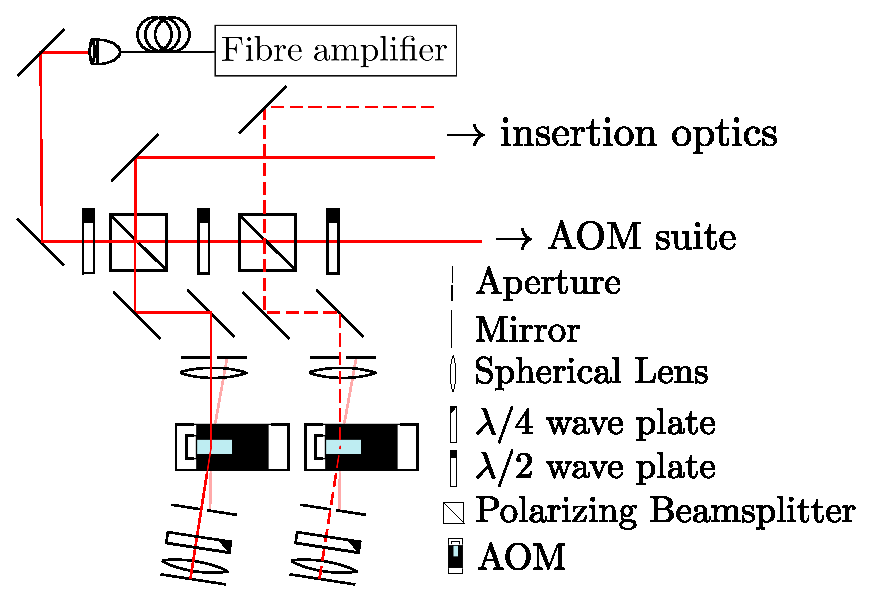
\includegraphics[width=\textwidth]{fig/lattice/distribution_optics}
		  {\fontsize{11}{13}
		  \begin{tabular}{l c c}
		  \hline\hline
		  Beam & Intensity & Detuning \\
		   & $(I_\textrm{sat})$ & ($\Gamma$) \\
		  \hline
		  Collimator &67& -5\\
		  Zeeman &92&-160 \\
		  MOT 1 &87 (Horz.)&-22 \\
		  		&110 (Vert.) & \\
		  Push &110&+3.3 \\
		  MOT 2 &37 (Horz.)& -33\\
		   &140,400 (Vert.)& \\
		  \hline
		  \end{tabular}}
	    \end{minipage}
	\end{figure}

	We had to align the collimator and Zeeman slower beams before the MOT could be built.
	Naturally, having set everything up perfectly the first time, the MOT was nowhere to be found.
	After some further tweaking, we obtained a visual signature of the MOT on the camera, a 1-2cm diameter smudge in the dark \footnote{We had to switch the room lights off to reduce scattered light in order to spot it.}.
	With some life breathed back into the old machine, it was time for a much larger operation.


\subsection{Vacuum build}

	
	The first stage of the build was to assemble the new science chamber.
	As we were waiting on delivery of the multichannel plates (MCPs) for the final detector, we assembled the second science chamber in order to get the low-velocity intense source (LVIS) operational in the interim.
	The first iteration of this build, prior to the addition of the MOT coils and optics, is shown in Fig. \ref{fig:first_build}.
	The large chamber (manufactured by Kimball physics) features two 8" windows on the flat sides through which the vertical MOT beams and absorption imaging are inserted, and 4.5" windows for insertion of the dipole beams on the top and side opposite the LVIS.
	Several $\frac{1}{2}$" ports are used as feed-throughs for in-vacuum instruments (namely a channel electron multiplier \emph{a.k.a.} channeltron for detecting ions produced by Penning ionization, a non-evaporative getter (NEG) to increase hydrogen adsorption and improve the vacuum, and a Faraday cup on a rotation stage to measure the flux of metastable atoms into the chamber via the LVIS) or covered with windows for optical instruments such as a photodiode to measure fluorescence of the trap.
	The lower assembly includes four-way and six-way crosses (6" flanges each).
	The four-way cross featured a turbomolecular pump (opposite the point of view) which was backed by roughing pump.
	The six-way cross (at the bottom of the stack) featured a residual gas analyser (RGA), whose purpose is described below.
	The entire assembly was put together while supported by four jack stands (one on each horizontal flange of the six-way cross) on a pallet jack.
	The pallet jack could then be wheeled into position and raised to height, and then carefully docked with the back of the gate valve on the MOT.
	The apparatus also featured an old discrete dynode electron multiplier (manufactured by ETP) that was used in early attempts to detect atoms dropped from a magnetic trap, but later stopped working and was thus of no use as a diagnostic for the optical dipole trap.

	The `push' beam was aligned by maximizing the flux from the first MOT into the science chamber as measured by the current on a Faraday cup.
	The sensor was positioned so that it could rotate into the helium beamline from its resting position out of any relevant optical paths.
	The current $I$ (in amps) gives an estimate of the order-of-magnitude flux $\phi_a$ of the atoms by the rule of thumb that $\phi_a\approx I/q$.
	This is an approximate method, but easily suffices for diagnostic purposes.
	Once we obtained a signal that the push beam was reading a current of order 200pA, indicating a flux on the order of 10$^9$ \mhe~atoms per second, we proceeded to assemble the rest of the vacuum system (shown in Fig. \ref{fig:underbelly}) and the MOT optics (detailed in section \ref{sec:new_optics}).
	The strategy was to assemble the MOT and absorption imaging systems to establish the magnetic and dipole traps, then use the ETP electron multiplier to optimize the dipole in the case we were still waiting on the MCP.
	The gate valve below the science chamber meant that we could close off the lower portion of the system and replace a single flange at the bottom of the 24" chamber when installing the MCP-DLD detector stack.
	Thus we would be able to perform the final upgrade without disturbing the MOT optics or breaking vacuum in the MOT chamber, which would be a significant advantage in that it would considerably simplify the necessary bake-out of the vacuum chamber, the subject of the next section.
	

	\begin{figure}
	  \begin{minipage}{0.55\textwidth} %4-8-16
	  \vspace{0pt}
			\includegraphics[width=\textwidth]{fig/lattice/science_chamber_internal}
		   {\begin{flushright}\caption{Initial build of the new science chamber.
	Right: The science chamber features a Faraday cup,  channeltron, and a NEG for vacuum maintenance.
	The camera was initially used to monitor the first MOT. Later uses of the camera are discussed in sections below.
	A 6" gate valve separates the chamber from a temporary assembly underneath the table.
	Top: Internal view of the chamber, taken the preceding day (after which the channeltron was moved to make room for the mounting plate, see below).}\label{fig:first_build}\end{flushright}}
	  \end{minipage}
	  \hfill
	  \begin{minipage}{0.45\textwidth}
	  \vspace{0pt}
		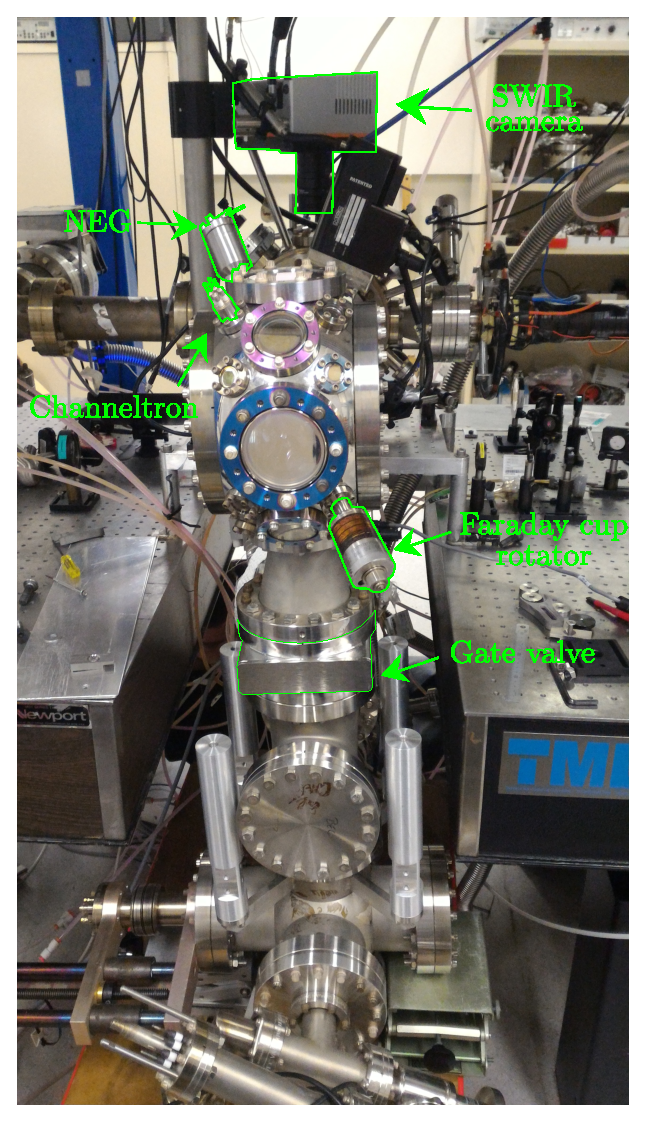
\includegraphics[width=\textwidth]{fig/lattice/science_chamber_profile}  % 5-8-16
	  \end{minipage}
	\end{figure}


	
	
	\begin{figure}
			\centering
		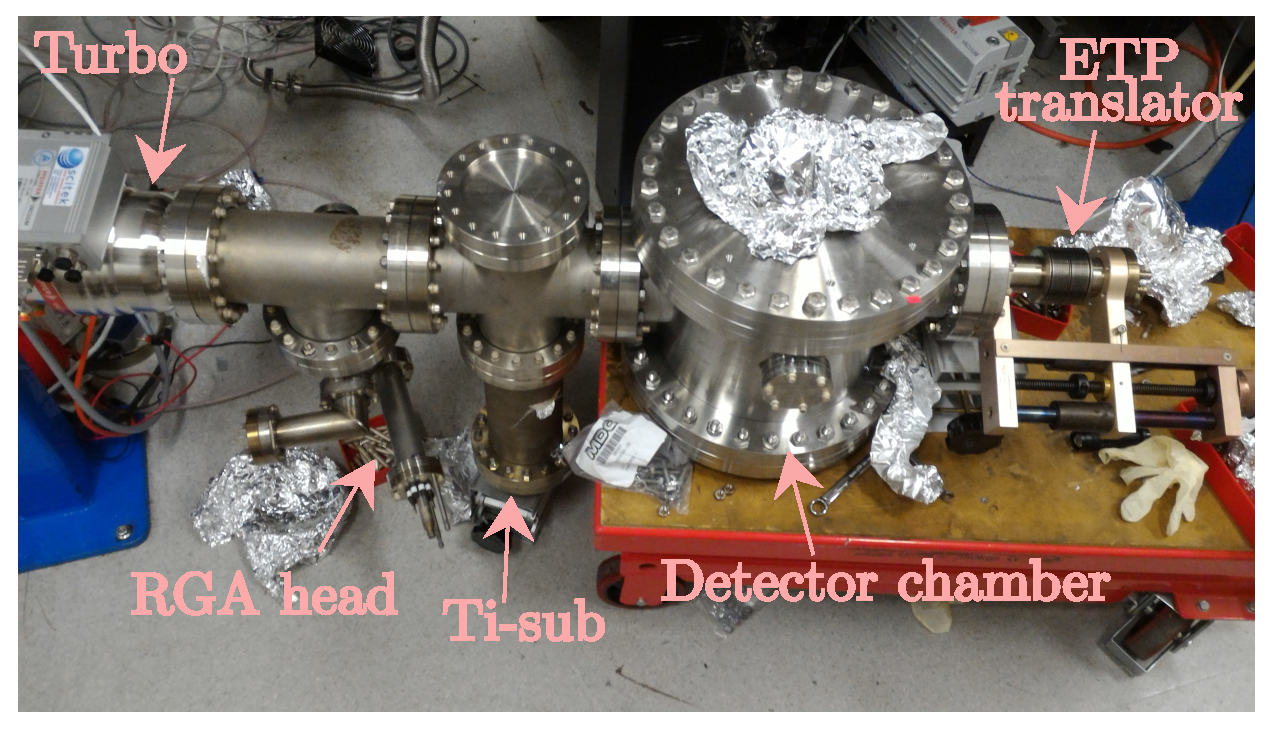
\includegraphics[width=\textwidth]{fig/lattice/detector_level.eps} %15-9-16
		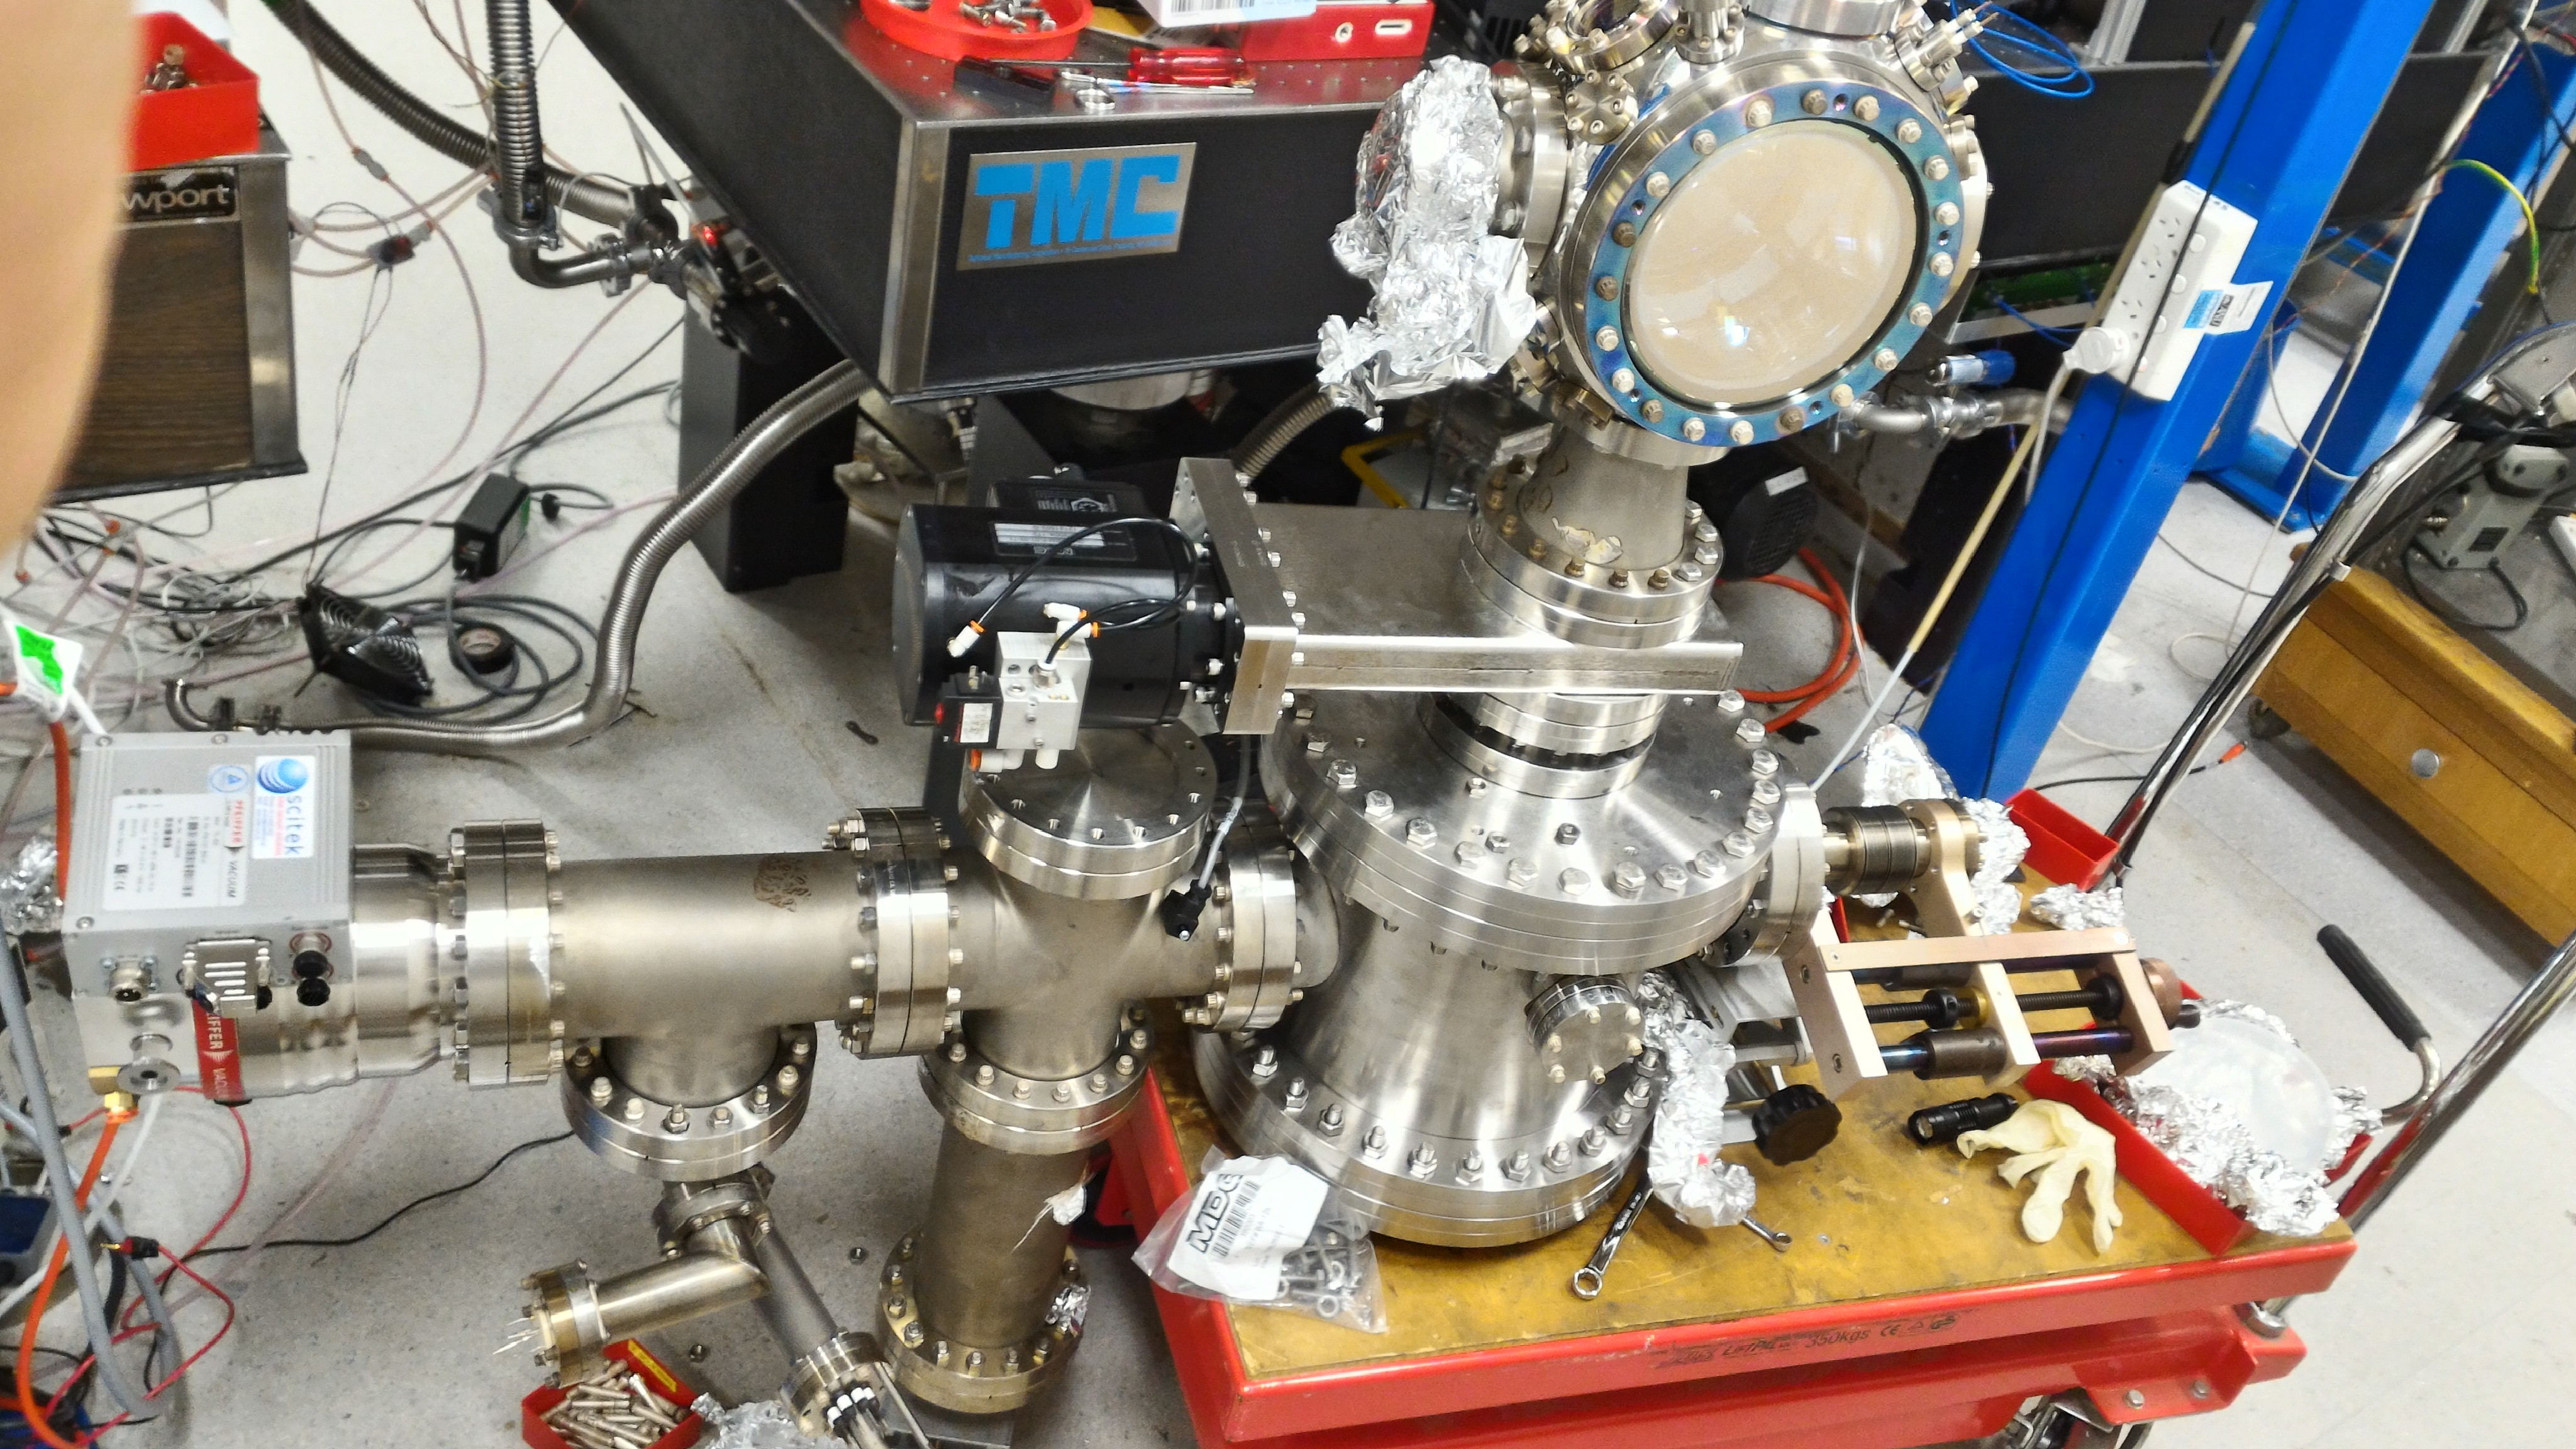
\includegraphics[width=\textwidth]{fig/lattice/full_assembly_20160915} %15-9-16
			\caption{Top: The leviathan-like underbelly of the science chamber resting after assembly on the mobile pallet jack and a smaller hand jack to support the TiSub.
		 Bottom: The science chamber was re-mounted with an intermediate gate valve and then wheeled into place.
		The assembly was stabilized on the blank flange at the bottom of the {24"}-diameter detector chamber, and by being \emph{really} heavy.}
	\label{fig:underbelly}
	\end{figure}

	


	
	\subsubsection{Improving vacuum conditions}

		As mentioned in chapter \ref{chap:apparatus}, the viability of cold-atom experiments depends on having a good quality vacuum.
		Any background gas molecules will typically have thermal velocities of several hundred m/s, with kinetic energies many orders of magnitude larger than the depth of the trapping potentials.
		Thus an overabundance of background gas can dramatically reduce the lifetime of magnetic and dipole traps, rendering evaporative cooling to degeneracy impossible.
		In the case of helium, there is the added issue of the small atomic mass and possibility of Penning ionization (even in low-momentum collisions) which only exacerbate the issue.
		This lab does not maintain cleanroom conditions outside of the optics tables, so even though care was taken to cover components in new foil when they were not being handled, some environmental pollution would be inevitable.
		Water is a common contaminant, but handling errors can also be a problem, and dust or aerosols can accumulate invisibly on the steel surface.
		All of these contaminants become problems when pumping down to vacuum as the pressure rapidly drops below the vapor pressure of many chemicals that may be stable in atmospheric conditions.
		These surface contaminants may outgas slowly (or be comparatively large) and lead to persistent `virtual leaks' in the chamber.
		The standard remedy is to wrap the machine in highly resistive wires insulated with fibreglass, cover it with aluminium foil to keep heat in, and bake the entire apparatus at around 150 degrees celsius for several days.
		The initial evacuation of the chamber by connecting the turbomolecular pumps was enough to observe a magnetic trap, but would be insufficient to make further progress (see Fig. \ref{fig:lifetime}).



		The higher temperature during the bake increases the outgassing rate and can even liberate some contaminants from the surface, allowing them to be pumped out by the turbomolecular pumps.
		In this process one typically observes a sharp rise in pressure as the chamber heats and the contaminants vaporise, and then a decrease to a lower steady-state pressure as the contaminants cease outgassing and the remnants are evacuated.
		Once the pressure stabilizes, the heater tapes can be turned off, and as the apparatus cools the pressure then settles to a steady-state value.
		An example of this procedure is illustrated in Fig.	\ref{fig:bakeouts}.
		The chemical makeup of gaseous contaminants can be determined using a residual gas analyser (RGA) which are essentially compact mass spectrometers.
		Figure \ref{fig:bakeouts} shows the partial-pressure contributions of gaseous contaminants before the first bake.
		
		Even after baking, the pressure may not be low enough to permit long-lived traps.
		Hydrogen leaching from the surface of the steel chamber can be significant, and even permeate the steel on long enough timescales.
		One means of addressing this is with a titanium sublimation pump (TiSub).
		This is not a pump \emph{per se} but rather a titanium filament.
		A pulsed current of $\approx5A$ (duty cycle approximately 30 seconds on, 60 seconds off) heats the filament and causes titanium to sublimate off the filament and adsorb onto the interior surface of the steel vacuum chamber.
		Hydrogen adsorbs to the titanium surface but not to steel, thus creating a `virtual pump' and driving the pressure further down.


		\begin{figure}
		% 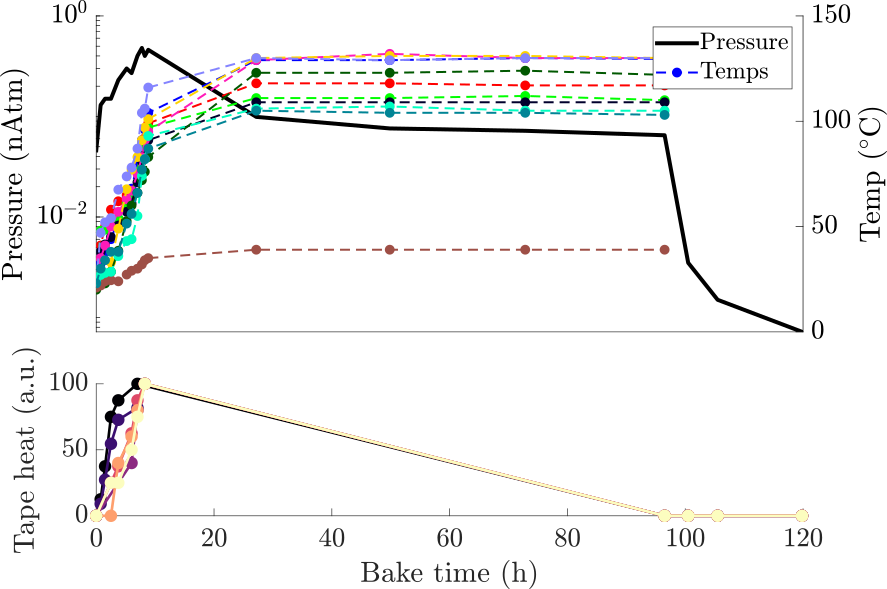
\includegraphics[width=0.5\textwidth]{fig/lattice/mid_december_bake_chart}
		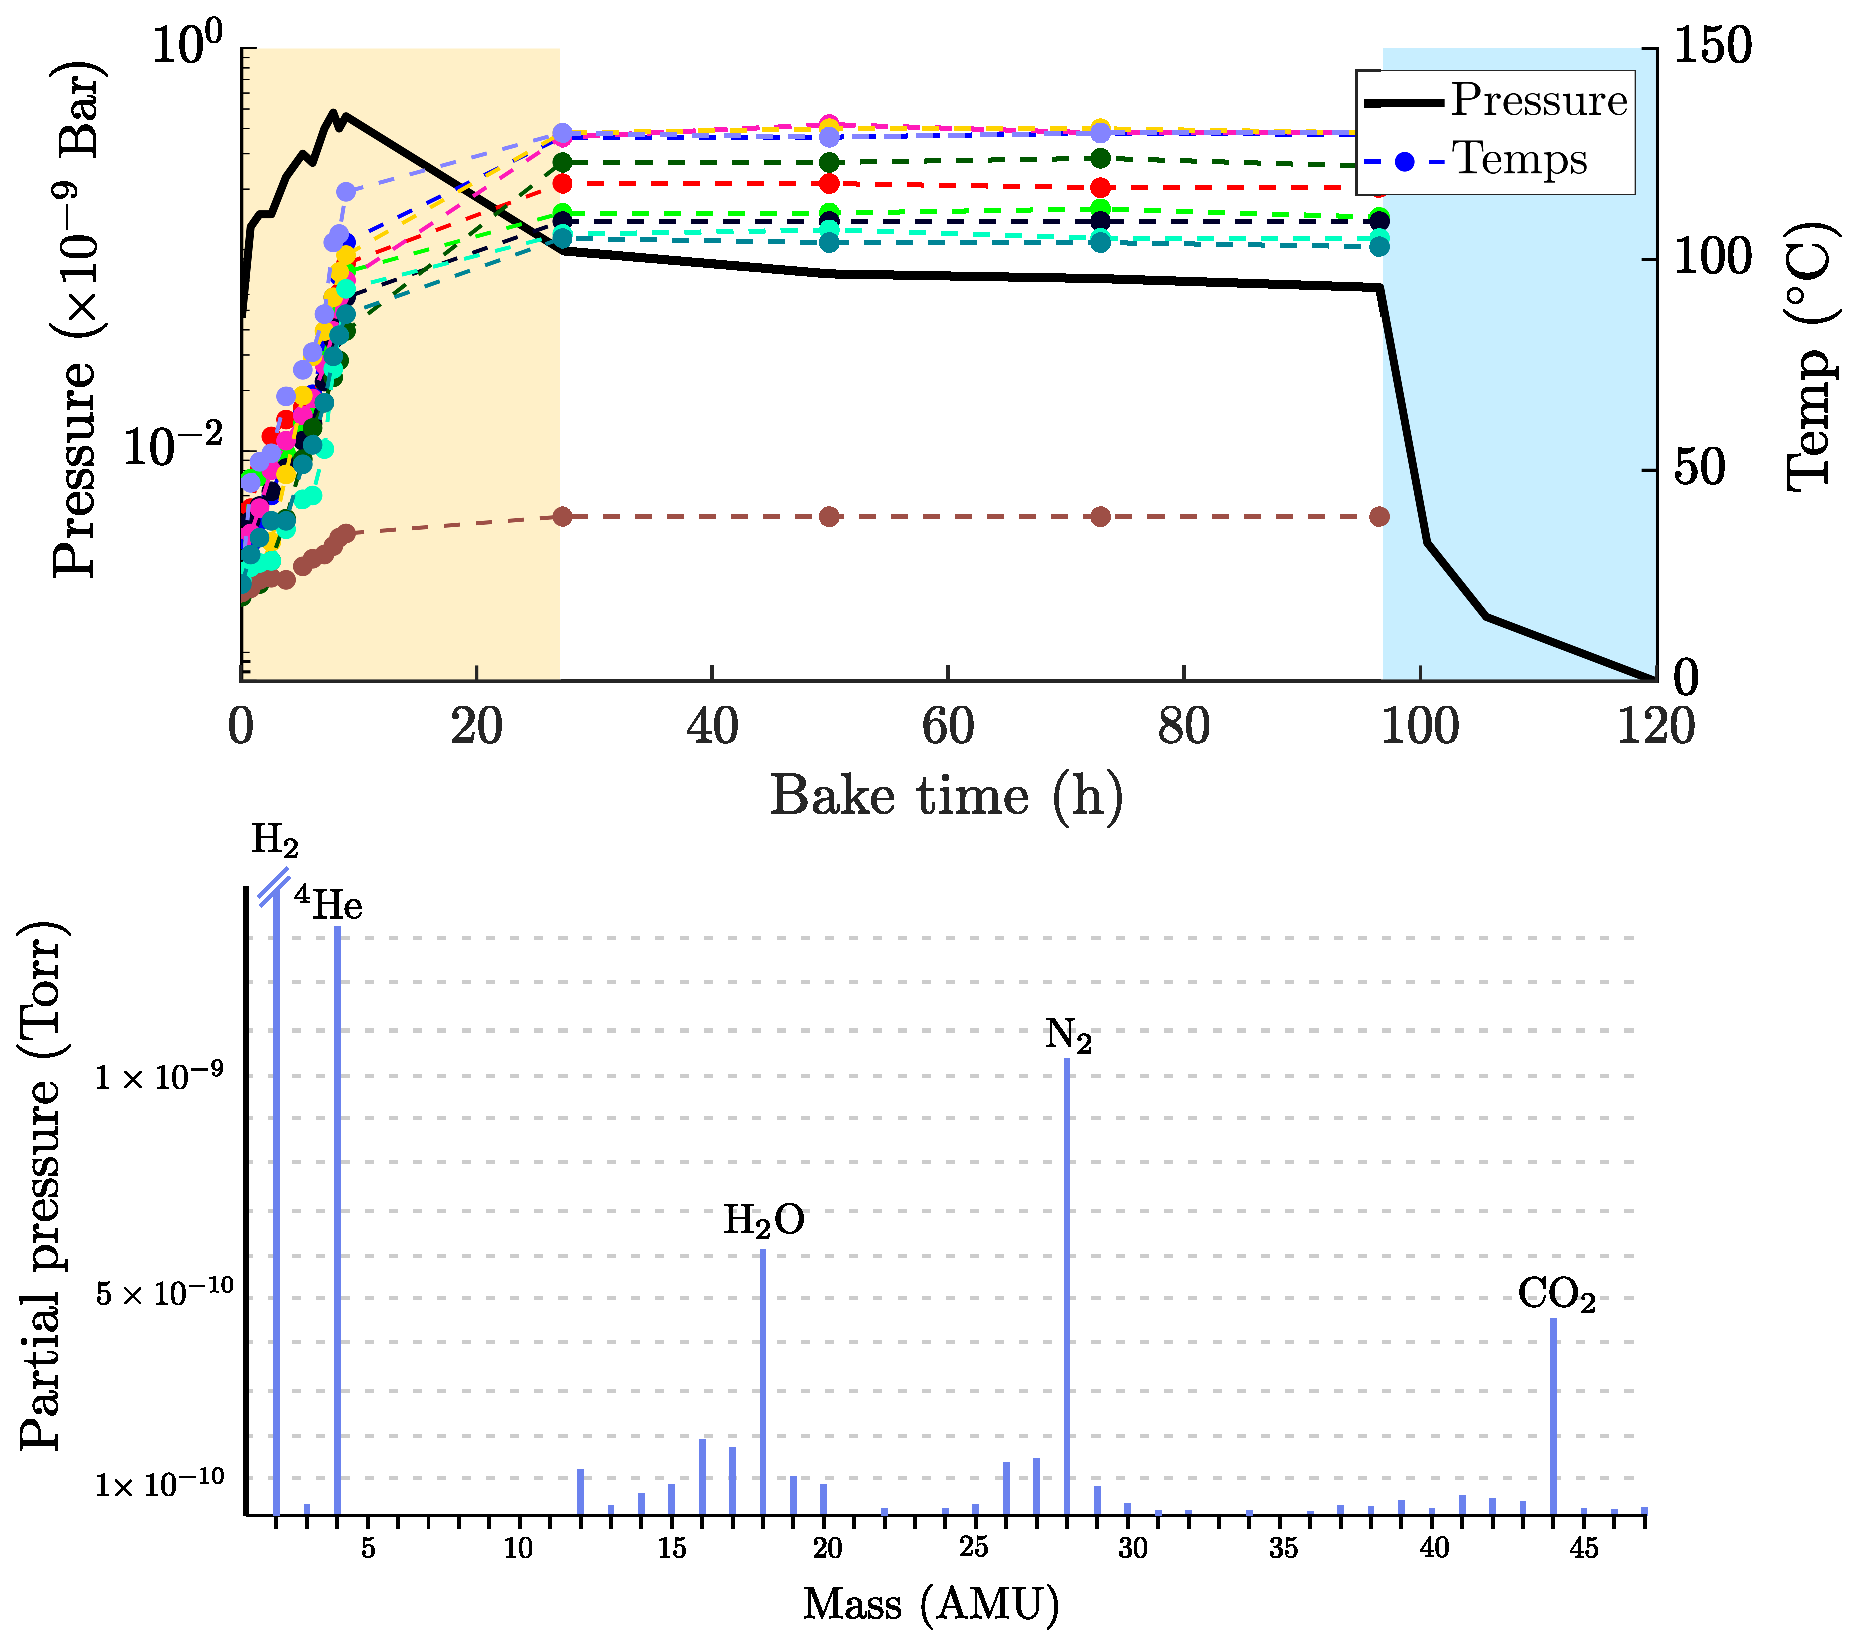
\includegraphics[width=\textwidth]{fig/lattice/RGA_pre_post_bake_nice}
		\caption{Top: The temperature measured by several thermocouples taped to the surface of the vacuum chamber (dots with dashed lines) and the pressure readout from the ion gauge on the science chamber during a bake.
		The heater tapes are supplied with current from variable voltage sources (variacs) which are turned up gradually to ensure even heating when starting the bake (orange region).
		After the tapes are switched off and the insulating foil opened, the steel quickly cools and the vacuum pressure stabilizes (blue region).
		The lower (brown) temperature curve was measured with a thermocouple on the flange connecting the 6" T-piece to the turbo (see Fig. \ref{fig:underbelly}) which was kept cool to avoid excessive heating of the turbo itself. 
		Lines in this figure are to guide the eye, individual measurements are denoted by the solid points.
		Bottom:
		Gas concentrations before the first bake as measured using the residual gas analyser (RGA).}
		% 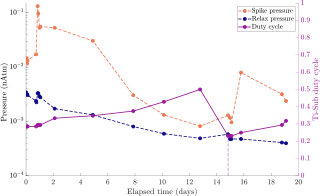
\includegraphics[width=0.9\textwidth]{fig/lattice/tisub_record}
		\label{fig:bakeouts}
		\end{figure}

	Another pressure reduction can be obtained by `getters' which operate in a variety of ways (a TiSub is a kind of hydrogen getter).
	In our machine we used a non-evaporative getter (NEG) in the science chamber.
	The NEG has a highly porous active area which adsorbs hydrogen very strongly.
	This means that they tend to carry in a lot of contaminants and have little remaining active area when first pumping down.
	We cleared the surface of the NEG by passing up to 5A of current through it.
	Again, the pressure spikes and eventually relaxes up to an hour later, when the current is switched off.
	As shown in Fig \ref{fig:bakeouts}, chamber bakes can improve the chamber pressure by up to three orders of magnitude.
	Afterwards, the TiSub can improve the pressure by a factor of five to ten, and the NEG by a factor of two to five.
		
	The payoff for this multi-stage procedure is the enormous reduction in background pressure that permits long-lived magnetic and (purely) optical traps.
	The lifetime can be quantified by any means that provides a reasonable proxy of the trapped population (the quantity of concern is the relative population at some time later), such as in Fig.	\ref{fig:lifetime}.
	Currently the machine operates at a background pressure below 3$\times10^{-11}$ mTorr (at which point the Ion gauge bottoms out).
		






\subsection{MOT and magnetic trap}
\label{sec:new_optics}

	\begin{figure}
		\includegraphics[width=\textwidth]{fig/lattice/science_chamber_oblique} %4-8-16
		\includegraphics[width=\textwidth]{fig/lattice/science_chamber_optics} %3-5-17
		\caption{The first iteration of the science chamber (in August 2016)  illustrating the coordinate axes used in the lab and the mounting surfaces for the magnetic coils (one of the Anti-Helmholtz (AH) coils was mounted on the back face of the large Kimball chamber). 
		The channeltron is visible on the lower right of the chamber (top), but was moved the next day to make room for the MOT mirror in a similar location in the later image.
		This configuration was used to test vacuum viability and align the LVIS.
		Once the new optic-mounting platform had ben constructed by technician Ross Tranter, we could install the MOT optics (bottom, mounting plate in lower-left quadrant).
		The MOT and imaging beam trajectories are marked, along with the direction of propagation of the LVIS.
		The Faraday cup and NEG are still installed in the lower picture, but the NEG is obscured by the chamber.}
		\label{fig:MOT_optics}
	\end{figure}
	% 1.7e8 atoms loaded at 2.5mK in 1 second, as measured using saturated fluro on an InGaAs PD [26]
	With a good, clean, vacuum and ample optical bench space around the science chamber, the optical components could finally be installed.
	Figure \ref{fig:MOT_optics} shows the enclosing construction around the science chamber that supports a MOT, magnetic trap, and absorption imaging.
	First, the magnetic coils were mounted on the windows to create the anti-Helmoltz field (with axis of symmetry along $x$, parallel to the Zeeman slower) and a bias field directed along the $y$ axis, back along the LVIS.
	The diagonal MOT beams enter through the 2$\frac{3}{4}$" widows on the 45$^\circ$ ports.
	We used the channeltron as a sensor for the presence of a MOT during initial alignment.
	A poorly-aligned MOT (or one with unfavourably set beam parameters) would not have been easily visible by camera or photodiode, but the increase in Penning ionization rate would in principle be controllable by blocking a laser beam and hence provide a fast diagnostic.
	The MOT itself could only be constructed after installing a mounting plate around the base of the vacuum chamber, which was installed after baking the entire new assembly.
	


	\begin{figure}
		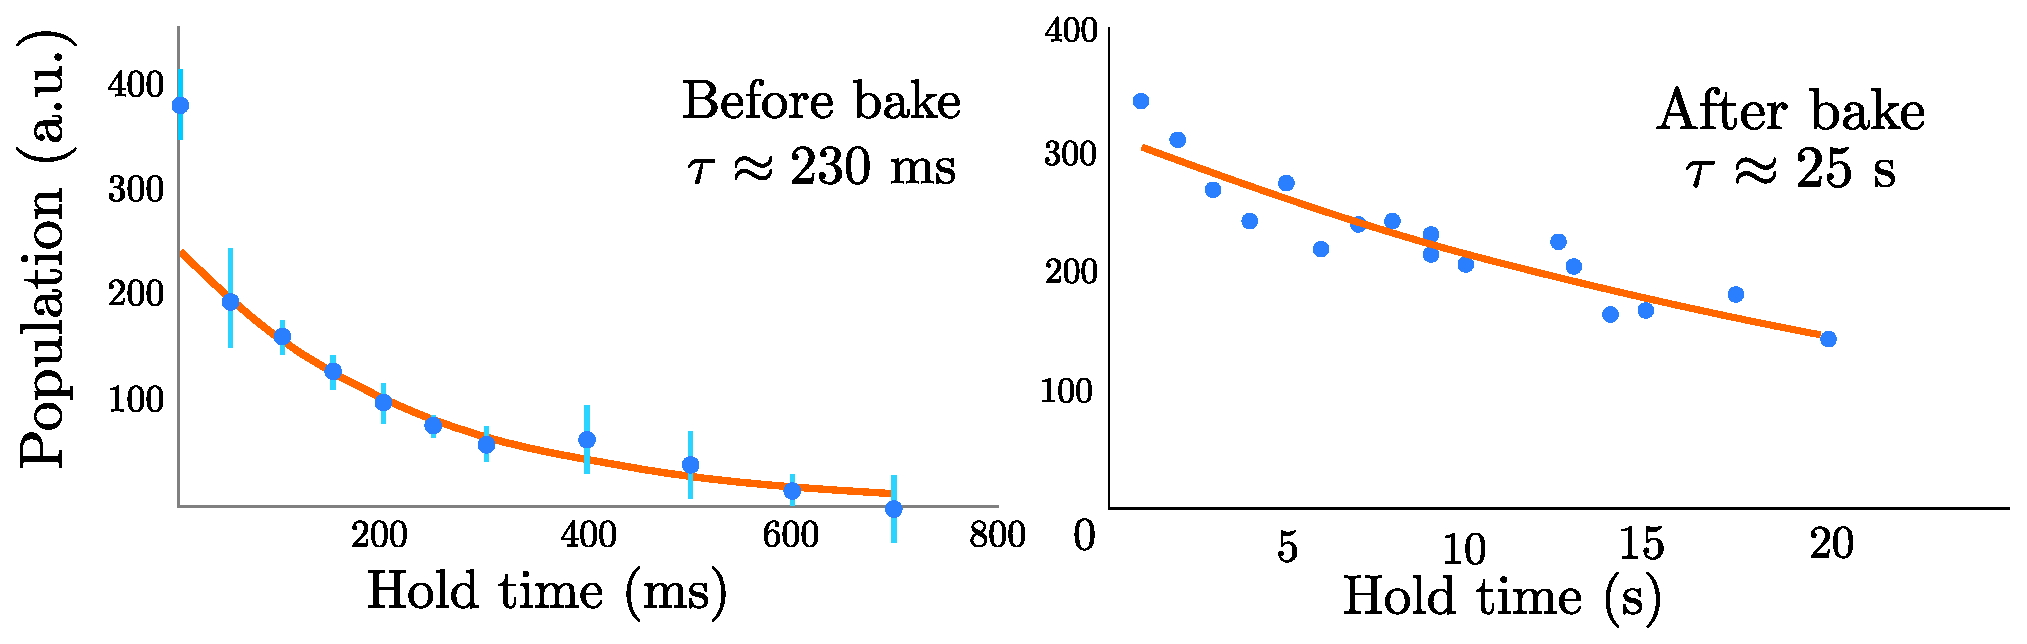
\includegraphics[width=\textwidth]{fig/lattice/trap_lifetimes}
		\caption{Magnetic trap lifetime measurements using before and after baking the new vacuum system. 
		The uncalibrated measurements only show the relative population, due to the measurement method described in section \ref{sec:abs_img}.
		Data points in the left plot are taken from averages of three shots, points on the right plot are single shots.
		The lines in both graphs are exponential fits.}
		\label{fig:lifetime}
	\end{figure}


\subsubsection{Absorption imaging}
\label{sec:abs_img}
		
	Alignment of the dipole trap was eventually made possible by absorption imaging.
	This system is preferred over the MCP-DLD for imaging MOTs and magnetic traps because 
	the clouds can be so wide on the detector that it is impossible to accurately determine the width, thus temperature, of the cloud.
	The analysis can be made more difficult by the potential saturation of the detector at large fluxes.
	A final, albeit lesser, concern is that MOTs and magnetic traps contain thousands of times as many atoms than remain after condensation and so they would shorten the detector's lifespan.
	% This imaging system now provides access to measurements of the temperature, density, atom number, and thus phase space density of a trapped cloud.
	

	\begin{figure}
	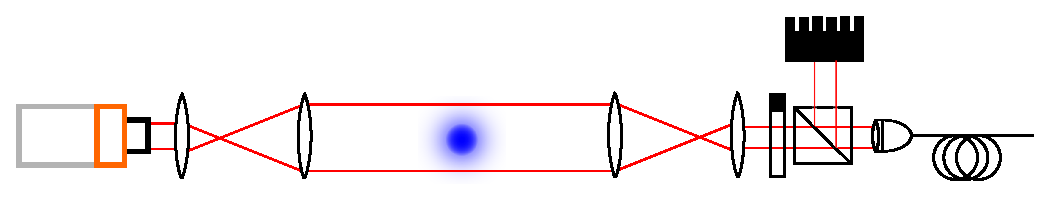
\includegraphics[width=\textwidth]{fig/lattice/abs_img}
	\begin{minipage}{0.44\textwidth}
	\vspace{0pt}
		\caption{ Above: Schematic of the absorption setup as described in the text.
		Adjacent: 
		Example image of the MOT.
		In practise the shot noise on the camera can be significant, and so for visual inspection a smoothing kernel is applied.
		Because of the issues in the text, it is nontrivial to make meaningful inferences about trap properties from in-trap images like these.}
		\label{fig:abs_img}
		\end{minipage}
		\hfill
		\begin{minipage}{0.54\textwidth}
	    \vspace{0pt}
	    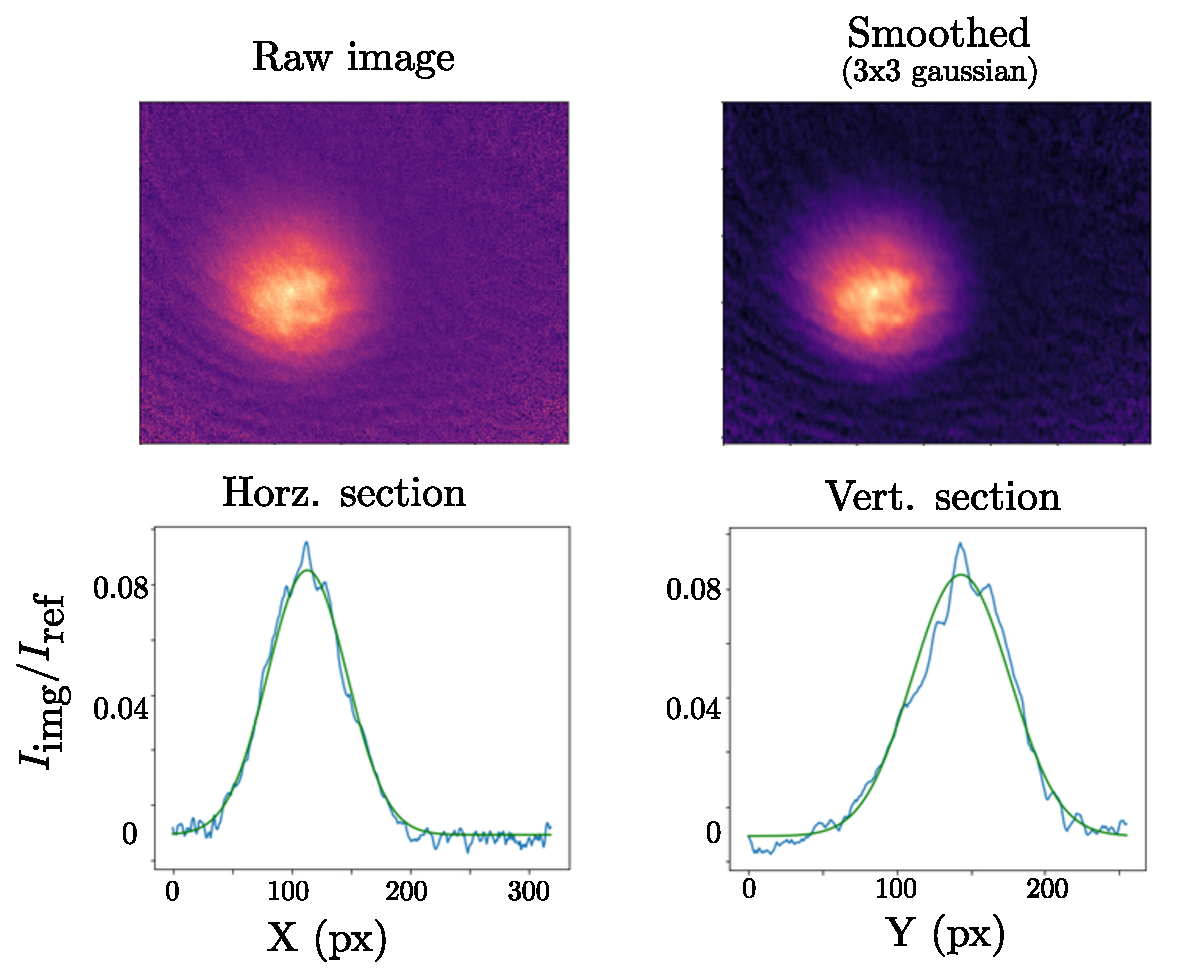
\includegraphics[width=\textwidth]{fig/lattice/20170606_CMOT_img}
	    \end{minipage}
	\end{figure}


	A simple description of absorption imaging is that one `takes a photo of the shadow of the atoms' by illuminating the sample with a collimated laser beam, and then projecting the beam onto a camera (Xenics Bobcat, 256x320 pixel InGaAs sensor, 20$\mu$m pixel pitch).	
	Detailed discussions of the physical principles and implementations of this technique are presented in \cite{MakingProbingUnderstanding,TychkovThesis}.
	Here we present a simple picture, and an illustration in Fig. \ref{fig:abs_img}.
	A laser tuned close to resonance with the atomic sample is coupled via optic fibre to the absorption imaging setup.
	The light passes through a polarizing beam splitter and then a half-wave plate to fix the polarization, which is useful when imaging in the presence of a bias field\footnote{And indeed the earth's field, which was later found to be strong enough to suppress Penning ionization sufficiently to achieve condensation \cite{Abbas21}.}.
	The beam is then magnified by a 4:1 telescope to a $\approx1$ cm collimated waist and directed at the atomic sample through the vacuum windows.
	The electric field on the exit side of the cloud will have been attenuated by a factor $Ae^{i\phi}$, where the attenuation factor $A=\exp(-\frac{\tilde{n}\sigma_0}{2}\frac{1}{1+\delta^2})$ depends on the column density  $\tilde{n} = \int n(x) dx$ (integrated along the beam axis), the detuning in (half-linewidths) $\delta=2(\omega-\omega_0)/\Gamma$, and the absorption cross-section which is $3\sigma_0\lambda^2/2\pi$ in the two-level approximation \cite{MakingProbingUnderstanding}.
	The phase $\phi$ also depends on the atomic density and detuning from resonance, and is in principle useful for techniques like phase contrast imaging, but is not presently used in this apparatus.

	The camera records an image during the application of the laser light and a second image of identical exposure time after a {$\approx$10 ms delay}\footnote{We found it helpful to ensure that the AOM switched off in the meantime as well, and turned back on for the same cycle time for the second measurement.
	The AOMs can exhibit slow rise-times to their steady state pointing and efficiency due to dissipation of heat into the crystal from the RF drive.
	This was measurable as differences in the light intensity between subsequent images if the AOM was left on between exposures.}
	By this point the atoms have scattered many photons and left the laser path.
	The second image is used as a reference to compute the integrated absorption at each pixel.
	A light-free image can be used as a `darkfield' to compensate for the camera's inherent noise profile.
	The ratio of (calibrated) pixel intensities in the presence of atoms $I_\textrm{abs}$ to the reference image without atoms $I_\textrm{ref}$ then provides a measure of the squared transmission coefficient,
	\begin{equation}
	A^2(x,y)=\frac{I_\textrm{abs}-I_\textrm{dark}}{I_\textrm{ref}-I_\textrm{dark}}.
	\end{equation}
	The 2D absorption profile can be fitted for purposes of further quantitative analysis. 
	Imaging in-trap is certainly possible and useful for optimizing performance, but it introduces the complication of a spatially-varying magnetic field.
	This means that the transmission coefficient varies due to the Zeeman shift around the trap.
	However, the initial imaging setup had too large a magnification to image the far-field density distribution which is necessary for thermometry.
	This design was shaped by the objective to load atoms into the dipole trap by using absorption imaging as the diagnostic, hence the magnification was chosen such that the MOT would almost fill the frame of the camera sensor.
	Therefore thermometry was not performed using this technique. 
	This was a shortcoming of the first design which was later remedied by upgrading the magnetic coils (see below), thus producing a more tightly-confining field and thus a denser trap.
	For detection and analysis of clouds released from a dipole trap, the lab currently uses the pulses of current across the MCP plates to infer the time-of-flight of atomic detection events \cite{Abbas21}.
	Calibration of the DLD for reconstruction of spatial information is currently underway.

	We could still perform (approximate) population measurements by fitting a Gaussian profile to the images.
	Unfortunately this was not adequately sensitive to measure the lifetime of the magnetic trap.
	After a short decay time it became impossible to get a good fit or even to see the cloud by eye in the absorption images, and thus the long-time behaviour was inaccessible.
	Instead, we released atoms by turning off the magnetic trap and used the number of detection events from the electron multiplier (manufactured by ETP) as a proxy for the population. 
	The current pulses resulting from atoms landing on electron multiplier were passed through a constant fraction discriminator, amplifier, and pulse rate counter which passed into the LabView software.
	The lifetime could then be obtained by an exponential fit to the measured populations over time.
	Measurements of the magnetic trap lifetime before and after the chamber bake are shown in Fig. \ref{fig:lifetime}.


	
	

\subsection{Dipole trap}
	While the main chamber was unworkable during bakeouts, construction could continue on other components of the machine, including the control and distribution systems for the optical dipole beams.
	These beams are generated by a 1550nm diode laser with a linewidth of $\approx100$ kHz that seeds a 30W fibre amplifier.
	The high-power beam is split into two AOM arms in a similar manner to the cooling optics described above.
	This configuration is illustrated  in Fig.	\ref{fig:dipole_optics}.
	% Because of the high power and stability demands, the optics were mounted on sturdier posts.
	
	To mitigate against misalignment of the dipole beams, which would eventually need to be overlapped in the focal region within less than 100 $\mu$m, we coupled light from the generation optics to the shaping optics via high-power NKT Photonics photonic crystal fibres to ensure the downstream optics are independent of the alignment upstream.
	Each AOM was driven at a fixed frequency by an amplified voltage-controlled oscillator, but the drive power was set in closed-loop configuration (in contrast to the cooling optics) to mitigate against heating the trap through intensity fluctuations.
	The voltage from a post-fibre photodiode was returned to a PID controller whose set point was determined by an arbitrary waveform generator pre-loaded with user defined waveforms and triggered by the main DAQ system.
	After losses in AOM transmission efficiency and fibre coupling losses, the maximum achievable (total) efficiency of each arm was about 30\% (defined as the ratio of power delivered into the chamber over the input power to the respective AOM).
	While I was working in the lab, the beam powers were roughly equal, but in the interim the dipole system has been redesigned, as discussed in \cite{Abbas21}.

	
	
	\begin{figure}
		\centering
		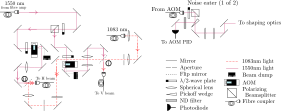
\includegraphics[width=\textwidth]{fig/lattice/dipole_optics}
		\caption{Schematic of the 1550nm optics used to generate and control the dipole trap beams in the lattice machine.
		The AOMs are used for amplitude control and fast switching, and to run the dipole beams at slightly different frequencies to avoid mutual interference.
		They are driven by dedicated PID controls set in configurable sequences with the arbitrary-waveform generators.
		The beams then focus into an optical fibre which transports the beam to the shaping optics (example on top right).
		Initial alignment of the dipole beams is achieved one beam at a time by inserting one of the removable mirrors (marked (i) and (ii)) and coupling resonant 1083nm light into the fibre.}
		\label{fig:dipole_optics}
	\end{figure}
	

	It is generally desirable to operate far-red-detuned dipole traps at very high intensities to create deeper traps (recall the ground-state shift scales with the intensity $I$, c.f. chapter \ref{chap:theory}).
	Deeper optical dipole traps can contain more atoms at a given temperature by virtue of trapping over a larger range of particle momenta, and so greater laser intensity is generally a good thing.
	It is true that spontaneous off-resonant scattering rates increase (approximately linearly) with intensity, but this can be remedied by detuning further (the scattering rate falls off with $\Delta^2$).
	Therefore one can obtain better loading efficiencies by using brighter beams.
	The purpose of the shaping optics are thus to shape the profile of the beam such that it reaches a tight focus.
	In order to achieve this, given the non-collimated laser profile emitted from the fibres, we first had to determine the profile of the beam, and then determine an arrangement of lenses to shape the beam to a tight focus at the desired trap location.
	The procedure we used to construct the shaping and insertion optics are discussed here.
	We aligned the beam output from the fibre parallel to a 1m-long rail which would be used to mount the lenses.
	We measured the profiles (at low power) by taking images with an InGaAs camera and fitting the output images with 2D gaussian profiles .
	A constrained two-dimensional Gaussian fit yields the waists $\sigma_x$ and $\sigma_y$ along the frame axes.

	A collection of measurements of the waists at positions $z_i$ along the rail can be fitted by the expression $w(z) = w(0)\sqrt{1 + (z/z_R)^2}$ for the waist of a Gaussian beam.
	In the preceding expression, $w(z)$ is the beam waist at distance $z$ from the focus and $z_R=\pi w(0)^2n/\lambda$ is the Rayleigh range (in terms of the laser wavelength $\lambda$ and refractive index $n$).
	We can then calculate the complex beam parameter $q(z) = z + i z_R$ and propagate it backward to determine the spot size and radius of curvature at the beginning of the rail.
	We used these values as input to a home-coded optical simulator which predicts the beam waist at a position $z$ after the beam propagates through a user-defined set of lenses and total optical path length.
	An example of such a simulated beam profile is shown in Fig. \ref{fig:profiling}.
	In reality some manual adjustment is necessary.
	The focus was finessed by deflecting the beam along a path of equal length to the distance to the desired trap centre and focusing the beam with respect to a camera at that position.

	\begin{figure}
	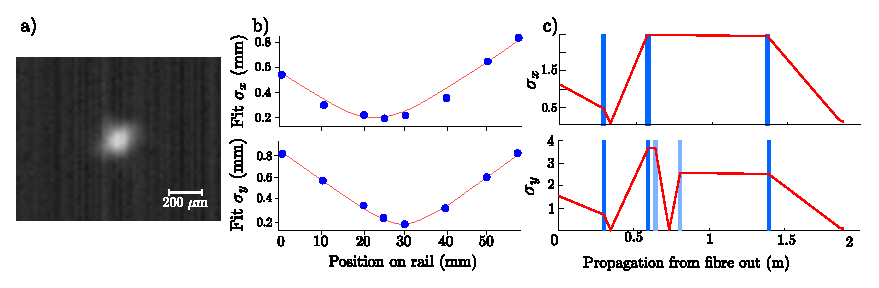
\includegraphics[width=\textwidth]{fig/lattice/dipole_profle_combo}
	\caption{a) Image taken from the InGaAs camera near the focus of a dipole beam.
	b) Beam waists along the rail as obtained from two-dimensional Gaussian fits to the images.
	c) Forward-propagation simulation of the beam waists which was designed to reshape the profiles.
	Cylindrical lenses only act on one of the axes, and are shown in a lighter blue.
	This iterative process produced the image on the left, with waist sizes 130$\mu$m and 124$\mu$m.}
	\label{fig:profiling}
	\end{figure}



\subsubsection{Dipole trap}
\label{sec:dipole_trap}

	The dipole beams were first aligned to overlap with the magnetic trap by piping resonant light (at 1083 nm) through the dipole beam delivery fibres instead of 1550 nm.
	To do this, we redirected a few mW of light from the absorption imaging optics using a beamsplitter, passed it through an attenuator, and inserted it into the dipole optics via removable mirrors as illustrated in Fig.	\ref{fig:dipole_optics}.
	The endgame strategy was to achieve BEC by evaporative cooling in an optical dipole trap composed of two beams intersecting at right angles.
	Given total efficiencies of about 30\% through the dipole optics, we could deliver about 5W of power through each beam.
	With each beam focused to a waist of order 100$ \mu$m, the peak intensity of each beam would be $I_0 = 2P/\pi w_x w_y \approx 3.5\times10^9$ mW cm$^{-2}$, and combine to give a dipole trap about 70 $\mu$K deep.
	This highlights the need for very cold magnetic traps (and tightly-focused dipole beams) to ensure many atoms have sufficiently low energy to remain in the dipole trap.
	One also desires a tightly-confined magnetic trap to ensure good spatial overlap of the magnetic trap with the brightest parts of the dipole beam.
	Furthermore, the rate of elastic collisions between trapped atoms increases with tighter traps, which permits more efficient evaporative cooling \cite{Ketterle96}, underscoring the need for tight traps.
	Several iterations of magnetic field configurations and RF ramps were tried during the build but no significant improvement in loading efficiency (based on absorption-imaging measurements) was obtained.
	Due to the aforementioned issues with time-of-flight imaging given the small field of view, the challenges of in-trap imaging, and the low loading efficiency of the dipole trap, precise thermometry was not yet possible.  
	In the end, a key step forward was to install in-vacuum coils (at no small expense of effort) after I had left the lab.
	Details about the present trapping methods are presented in \cite{Abbas21}.
	This includes several re-assemblies of the optics and a change in the dipole trap configuration (namely switching to a second horizontal beam rather than a vertical beam as the upper flange of the Kimball chamber now hosts the coil feed-throughs including their cooling water).
	


	\begin{figure}
		\begin{minipage}{0.43\textwidth}
		\vspace{0cm}
		\caption{The $y$-axis dipole passes through a final focusing lens (lower middle) and is lifted by sturdy optics mounted to a heavy post.
	The upper mirror dials can be remotely controlled, using piezo-driven stepper motors, for precision alignment.
	The camera and refocusing optics for the absorption imaging system are just outside the left of the frame.}
		\label{fig:lifetime}
		\end{minipage}
		\hfill
		\begin{minipage}{0.55\textwidth}
		\vspace{0cm}
		\includegraphics[width=\textwidth]{fig/lattice/dipole_insertion_mirror} %20-11-17
		\end{minipage}
	\end{figure}


	
	However, the basic operation of the dipole is unchanged, including the alignment procedure we discovered, and so is documented here.
	As discussed above, the alignment procedure used resonant light, directed through the dipole fibre into the trap.
	Coarse alignment could be found by supplying light near resonance through the dipole optics after loading a magnetic trap, and optimizing for the destruction of the cloud in response to the beam.
	Alignment could be finessed by reducing the intensity until the cloud recovers, then re-adjusting the beam to hit the centre of the trap and destroy it again.
	The cycle could be repeated until very low intensities were able to destroy the trap.
	Unfortunately we eventually found that there were multiple such optima.
	We determined that these were due to reflections of the beam from the inside of the chamber and scattering back across the trap.
	Afterwards, we acquired the image coincident with the resonant beam (rather than afterward) and found that when the beam intensity was reduced to a mere 4$\mu$W, the beam appeared to bore a hole through the cloud, as shown in Fig.	\ref{fig:dipole_align}.
	
	\begin{figure}
	\centering
	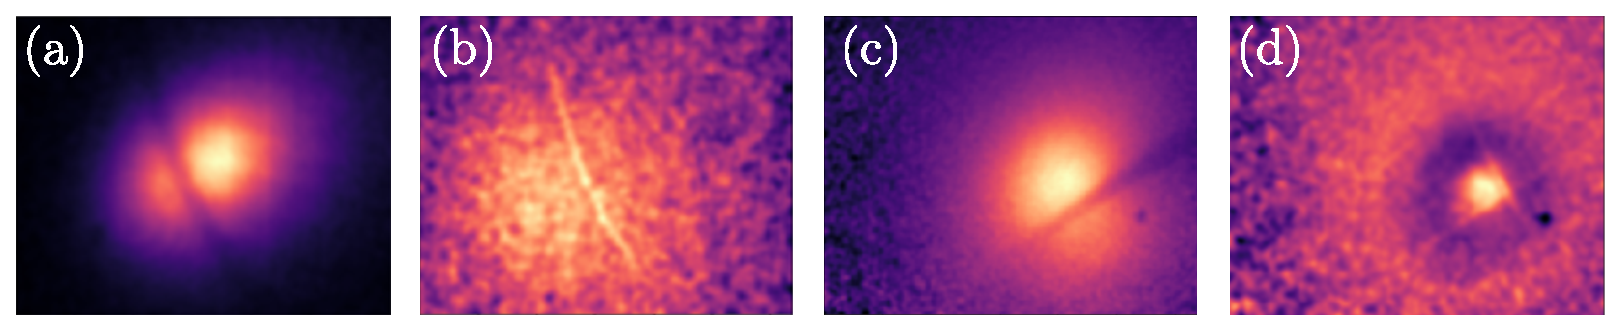
\includegraphics[width=\textwidth]{fig/lattice/dipole_alignment_stages}
		\caption{Stages of dipole beam alignment.
	The first alignment was achieved by passing resonant light through the cloud (a) and triggering the image acquisition (for 10 $\mu$s) at the same time as the resonant pulse.
	After switching to 1550nm light, the beam deflected slightly due to chromatic aberration in the optics (b) and could then be resolved in averages of 8-10 images. 
	The beam appears to bend in these images because the imaging beam was not aligned with the optical axis of the lenses, which was discovered and corrected using this technique.
	Some time later the vertical dipole was aligned using the same method (c) and so two dipoles could be loaded simultaneously. 
	Finally, an image of the combined magnetic and dipole traps could be taken ((d), average of 10 shots). To obtain this image, a Gaussian fit to the central cloud was subtracted from the image, with a residual halo and bright spot (c.f. the aforementioned issues with in-trap imaging).}
	\label{fig:dipole_align}
	\end{figure}

	After this initial alignment several attempts were made to optimize the dipole loading by adjusting the final lens position, mirror orientation, and experimental control sequences.	
	Matters were made more difficult by several concurrent issues.
	For one, we were \emph{still} waiting for parts for the MCP-DLD detector mount, the ETP electron multiplier had since failed, and the channeltron showed only modest changes in the ionization rate as a function of beam positioning.	
	This left absorption imaging as the sole means of ascertaining the loading efficiency.
	Unfortunately the signal-to-noise was poor and the dipole would only resolve after $\approx 8$ shots.
	At the time the experimental cycle was on the order of 15 seconds, and the long acquistion times were a major obstacle.
	It would eventually be found that the magnetic trap was simply not tight enough.
	The magnetic field gradient would later be improved by upgrade to in-vacuum coils during the tenure of the students who took up the mantle.
	

\section{Progress and outlook}
	


	After my departure, the lab sat motionless for some months as I had been the sole graduate student on the project.
	Later, the \mhe~lattice team was renewed by two PhD students (A. H.	Abbas and X. Meng) and a Masters student (R. S. Patil).
	The team has since achieved a BEC production time of as low as 3.3 seconds, nearly a factor of 2 faster than the prior art \cite{Bouton15} and a factor of 8 faster than the BiQUIC machine.
	The subsequent publication \cite{Abbas21} contains details about the new coils, additional infrastructure and cooling techniques, and characterization techniques.
	The large condensates, containing something on the order of a million atoms, are also competitive with the state-of-the art.
	I take my hat off to the students who picked up the trail where I had left off, and accomplished a goal I'd struggled towards for two years.


	Ahead, the team is faced with the challenge of aligning and optimizing three pairs of lattice beams.
	Once this is accomplished, there is still much ground to cover in exploring the Bose-Hubbard model.
	For instance, the time evolution of the system following a quench or sudden change in dimensionality would be a natural starting point.
	The onset of coherence could be probed via many-particle mometum correlations, extending the work in \cite{Carcy19} into the dynamical regime.	
	Beyond the Bose-Hubbard model, there lies a fork in the road.
	One path leads to the Fermi-Hubbard model by way of further infrastructure upgrades to achieve degenerate $^3$\mhe~in the same machine.
	The expertise gained through the ongoing upgrade of the BiQUIC machine to include $^3$He circulation would be instrumental in this mission.
	The other path is towards the study of the disordered Bose-Hubbard model (also known as the Aubry-Andr\'{e} model), which has been studied in quantum gas microscopes \cite{Rispoli19} but not, so far, with a momentum microscope.
	Theoretical studies predict that momentum-space localization occures in disordered lattices generated by lasers with incommensurate wavelengths \cite{Larcher11}, which is an aspect of localization which has received little attention.
	\vfill
	\begin{flushright}
	\singlespacing
	\emph{``It is not necessary to succeed in order to persevere.\\
	As long as there is a margin of hope, however narrow, \\
	we have no choice but to base all our actions on that margin"}\\
	- Leo Szilard\footnote{\emph{LIFE magazine} volume 51, issue 9, 1961 }\\
	\end{flushright}
	\onehalfspacing

	
% \part{Experiments with ultracold metastable helium atoms}
% % New papers to check out

% @article{PhysRevA.103.032810,
%   title = {Magic wavelengths for the helium $2{\phantom{\rule{0.16em}{0ex}}}^{3}{S}_{1}\ensuremath{\rightarrow}2{\phantom{\rule{0.16em}{0ex}}}^{1}{P}_{1}$ forbidden transition},
%   author = {Zhang, Yong-Hui and Tang, Li-Yan and Zhang, Jun-Yi and Shi, Ting-Yun},
%   journal = {Phys.
	% Rev.
	% A},
%   volume = {103},
%   issue = {3},
%   pages = {032810},
%   numpages = {7},
%   year = {2021},
%   month = {Mar},
%   publisher = {American Physical Society},
%   doi = {10.1103/PhysRevA.103.032810},
%   url = {https://link.aps.org/doi/10.1103/PhysRevA.103.032810}
% }




% https://arxiv.org/pdf/2103.14365.pdf

% https://www.sciencedirect.com/science/article/abs/pii/S0009261421003237
%  doubly excited states of He
\chapter{Frequency measurements of resonances between the second and fifth manifolds in {$^4$}\mhe}
\markboth{\thechapter. TRANSITION FREQUENCY MEASUREMENTS}{}
\label{chap:transitions}

\blankfootnote{The contents of this chapter relate to the work published in \textbf{Frequency measurements of transitions from the $2\triplet P_2$ state to the $5\singlet D_2$, $5\triplet S_1$, and $5\triplet D$ states in ultracold helium} by J. A. Ross, K. F. Thomas, B. M. Henson, D. Cocks, K. G. H. Baldwin, S. S. Hodgman, A. Truscott, \href{https://journals.aps.org/pra/abstract/10.1103/PhysRevA.102.042804}{\emph{Physical Review A} \textbf{102}} (2020)}




  {The} appearance of ordinary matter arises from interactions between charged particles and light.
	This phenomenon is the domain of the theory of quantum electrodynamics (QED), which provides the most accurate quantitative predictions of any physical theory to date.
	The theory of QED is the workhorse of modern atomic structure calculations, whose only inputs are the CODATA values of three physical constants: the proton-electron mass ratio, the Rydberg constant, and the fine structure constant $\alpha$.
	These constants of nature can be constrained with state-of-the-art atomic spectroscopy, which is accurate enough to match theoretical uncertainties in table-top experiments.
	Thanks to the quality of modern theory and experiment, atomic structure measurements reprise their role in frontier tests of physics.
	

  In 1964 Schwartz proposed the determination of $\alpha$ from the fine structure intervals of the $2\triplet P$ manifold in helium \cite{Schwartz64}, which are subject to strong QED effects.
	The contemporary knowledge of helium's structure greatly exceeds Schwartz's anticipation of parts-per-million accuracy.
	For example, the $2\triplet S_1 - 2\triplet P$ and $2\triplet P - 3\triplet D$ intervals measured by Cancio Pastor \textit{et al.} \cite{Pastor04} and Luo \emph{et al.} \cite{Luo15}, respectively, both have relative uncertainties better than 50 parts per \emph{trillion}, providing Lamb shift measurements accurate to several ppm.
	The measurement of the $\PStateManifold$ fine structure splitting by Smiciklas \textit{et al.} to sub-kilohertz precision determines $\alpha$ to several ppb \cite{Smiciklas10}.
	Measurements of the $2^{3\!}P_1-2^{3\!}P_2$ interval by Kato \emph{et al.}, accurate to 25Hz, would constrain $\alpha$ to less than one ppb given a similarly accurate measurement of the $2^{3\!}P_0 - 2^{3\!}P_1$ transition and QED calculations including terms of order $\alpha^7$ \cite{Kato18}.
	The corresponding QED calculations to seventh order have been completed \cite{Patkos21}. The authors note, however, that the predicted energies of the $2\triplet S - 3 \triplet D$ and $2\triplet P - 3 \triplet D$ transitions disagree significantly with experiments, and refrain from computing the nuclear charge radius until these discrepancies are resolved.
	

  \begin{figure}
  	
  	\begin{minipage}[t]{0.38\textwidth}
			\vspace{0pt}
      \caption{Energy level diagram for $^4$He showing the transitions measured in this work (blue) are driven by a tunable laser referred to in the text as the \emph{probe beam}.
				A laser tuned to the $2\triplet S_1-2\triplet P_2$ transition (red, referred to as \emph{pump beam}) populates the lower state of the target transitions.
				 The doubly forbidden $1^{1\!}S_0 - 2^{3\!}S_1$ transition is excited in a high voltage discharge source.
				Transitions across the dotted line are \emph{forbidden} by the $\Delta S=0$ selection rule.
				Level splittings are not to scale.}
      \label{fig:lvl_diag}
      \end{minipage}
      \hfill
      \begin{minipage}[t]{0.6\textwidth}
      \vspace{0pt}
      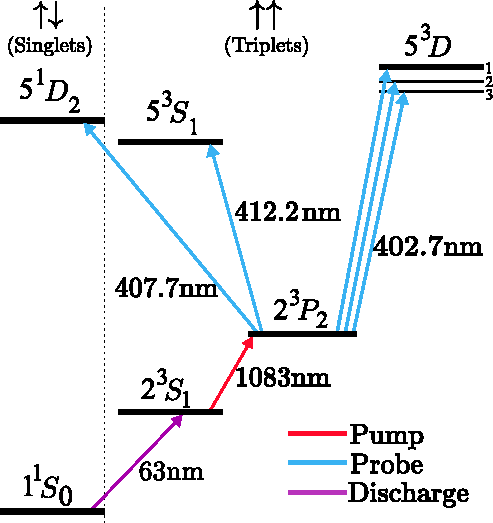
\includegraphics[width=\textwidth]{fig/spectroscopy/level-diagram-tight-latex-pdf.pdf}
      \end{minipage}
  \end{figure}

  A concurrent issue is the so-called `proton radius puzzle': Determinations of the proton charge radius from Lamb shift measurements in muonic and electronic hydrogen \cite{Pohl10, Bezginov19}, electron-hydrogen scattering experiments \cite{Beyer17,Xiong19}, and isotope shifts in light muonic atoms \cite{Kalinowski19,Pohl16} disagree significantly with both the CODATA recommended value and with other recent experiments \cite{Fleurbaey18}.
	 Helium is a promising candidate to provide insight into this unresolved issue because its simple structure is tractable to QED calculations.
	Ongoing theoretical work \cite{Pachucki15,Pachucki17,Pachucki11,Pachucki10,Morton12,Morton06,Patkos16,Patkos17} and recent high-precision measurements \cite{Rooij11,Notermans14,Notermans16,Rengelink18} find a $4\sigma$ discrepancy between the difference $\delta = r^2(^3\textrm{He}) - r^2(^4\textrm{He})$ of squared nuclear charge radii obtained from the isotope shifts of the $\MetastableState - \PStateManifold$ and ${2^{1\!}S_{0}} - \MetastableState$ transitions \cite{Pachucki15,Patkos17}.
	The completed calculation of QED effects to order $\alpha^7$ will allow determination of the absolute nuclear charge radii accurate to better than 1\% \cite{Pachucki17}.
	Along with these $\alpha^7$ contributions, measurement of the $2\triplet P-2\triplet S$ spacing to within 1.4kHz would allow a determination of the nuclear charge radius to below 0.1\% accuracy, better than expected from the muonic helium Lamb shift \cite{Wienczek19}.
	 
  Notable among recent studies of helium's structure are the measurements of \emph{forbidden} transitions between the singlet and triplet manifolds.
	Such transitions are made possible in reality due to relativistic effects and are extremely narrow, therefore precise measurements of their spectral features can provide stringent tests of QED \cite{Lach01}.
	The work in this chapter complements existing measurements of forbidden lines in helium at 1557nm \cite{Rooij11,Rengelink18}, 887nm \cite{Notermans14}, and 427nm \cite{Thomas20}.

	This chapter concerns frequency measurements of the transitions from the $2^3P_2$ state to five states in the $n=5$ manifold of $^4$He, illustrated in Fig.
	\ref{fig:lvl_diag}.
	Below, I describe the laser absorption spectroscopy technique we used to measure the energy intervals between the $2\triplet P_2$ level and five levels in the n = 5 manifold.
	These measurements improve on the precision of previous measurements by at least an order of magnitude \cite{Martin60}, and resolve the fine structure splitting of the $\PStateManifold_2 - 5\triplet D$ transition.
	Theoretical transition energies agree with the observed values within our experimental uncertainty.
	These include the first direct measurement of the spin-forbidden $2^{3\!}P_2 - 5^{1\!}D_2$ transition in helium, whose transition rate is four orders of magnitude smaller than the other transitions discussed here.  

\section{Measurement technique}

	The experimental sequence began with $\sim10^8$ atoms in the metastable $2\triplet S_1$ state, cooled to  $\sim1 \textrm{mK}$ in a magneto-optical trap, which were then transferred to a magnetic trap by switching off the light.
	Next, during the Doppler cooling stage, we illuminated the atoms with $\sim$30$\mu$W$/m^2$ of $\sigma^+$ polarized cooling light in an approximately uniform magnetic field set by the high bias of the BiQUIC coils, further cooling the atoms to $\sim200\mu \textrm{K}$ \com{Doesn't figure 5.5 show that the field is not uniform? }.
	Finally, forced evaporative cooling lowers the sample below the critical temperature to form a BEC.
	Each iteration of this procedure produced a BEC of $\sim 5\times10^5$ atoms in a cigar-shaped harmonic trap with trapping frequencies $\omega = 2\pi (425,425,45)$ Hz.
	To perform the absorption measurements, we disturbed the Doppler cooling stage by applying a probe beam tuned near the target transition, resulting in a reduction in the number of atoms cooled to degeneracy. 
	

	At the end of the experimental sequence a pulsed atom laser, described in section \ref{sec:atomlaser}, transfers $\sim$2\% of the trap population at a time to the untrapped $m_J=0$ state \cite{Manning10,Henson18_BCR}.
	The resulting coherent matter-wave pulses fall onto the detector, {depleting the entire trapped population after $\sim$200 pulses over 2 seconds.
	This allows}  the atom number and temperature to be accurately determined without saturating the detector.
	Our data collection protocol consisted of a cycle of one calibration shot with the probe beam switched off, followed by one measurement shot (with the probe beam on) at each of two magnetic field strengths used in the in-trap cooling stage.
	
	The physical basis of the measurement is the sensitivity of forced evaporative cooling to the initial conditions of the helium atoms.
	The precise effect of photon scattering on the final cloud properties depends on the exact details of the evaporation sequence, and is hard to model exactly.
	Instead, what follows is a qualitative picture of the role evaporative cooling plays in transforming photon scattering to a measurable change in trap population.

	During the Doppler cooling stage of BEC creation, the 1083nm cooling beam acts as an optical pump and excites atoms to the $2\triplet P_2(m_J=2)$ state.
	From the $2\triplet P_2$ state they may decay, with a lifetime of $\sim$97ns, back to the trapped metastable state or absorb photons from the probe beam and become excited again to the target state.
	Doubly-excited atoms may decay back to the trapped $m_J=+1$ state of the $2\triplet S_1$ level, in which case the photon absorption and emission events add heat to the cloud by imparting a nonzero average impulse to the atoms.
	This leads to an initially hotter cloud, which in turn reduces the efficiency of evaporative cooling, resulting in a higher atom loss during evaporation and a lower final number in the trap. Alternatively, atoms may decay to other untrapped magnetic states of the metastable state, or to the true ground state via a spin-flip transition to the singlet manifold.

	Decay to untrapped states reduces the initial atom number and can even impart heat to the cloud as these atoms leave the trap - via scattering with trapped atoms.
	This heating will be much smaller than in the previous case because the scattering rate will be small in such a dilute gas.
	However, reducing the initial trap population also manifests as a reduced final atom number.
	In both cases a photon scattering signal clearly manifests in the reduction of the total trapped final number $N$ relative to the final number $N_c$ in calibration shots.
	As such, the signal is defined to be the relative number loss $(N_c-N)/N_c$ to compensate for drift in the trap population over time.

\begin{figure}
      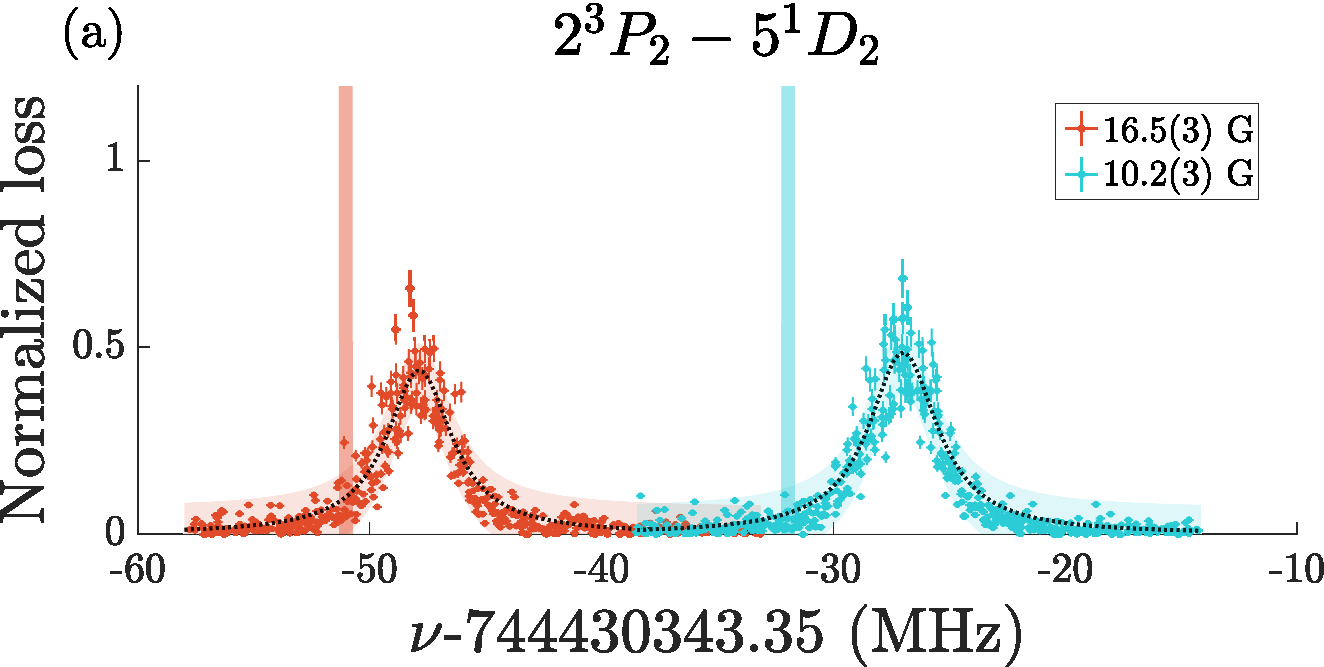
\includegraphics[width=\textwidth]{fig/spectroscopy/ci-plot-51D2.pdf}
    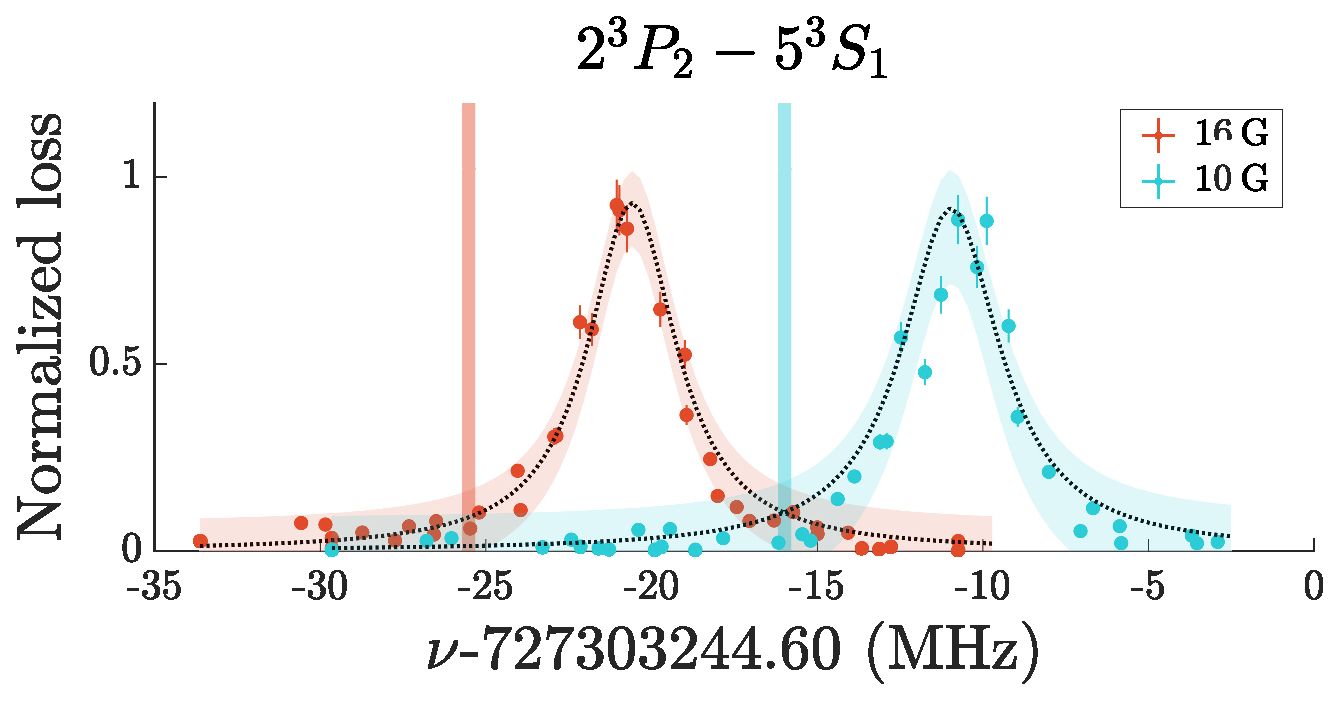
\includegraphics[width=\textwidth]{fig/spectroscopy/ci-plot-53S1}
   \caption{Line profile for (a) the spin-forbidden $\PStateManifold_2 -  5^{1\!}D_2$  and (b) the $2\triplet P_2 - 5\triplet S_1$  resonances, showing normalized atom number loss versus probe laser frequency $\nu$, as measured in a {16.5(3)}G (red) and {10.2(3)}G (blue) background field, with Lorentzian fits (black dotted line, with prediction confidence interval shaded).
	Error bars account for detector efficiency and calibration model uncertainty.
	For comparison, theoretical predictions (vertical bars) Zeeman shifted from the predicted zero-field value \cite{Drake07} according to the field calibration, whose uncertainty (shaded width) is dominated by background field measurements.}
    \label{fig:simple_lines}

\end{figure}


% \begin{figure}
%     \centering
%     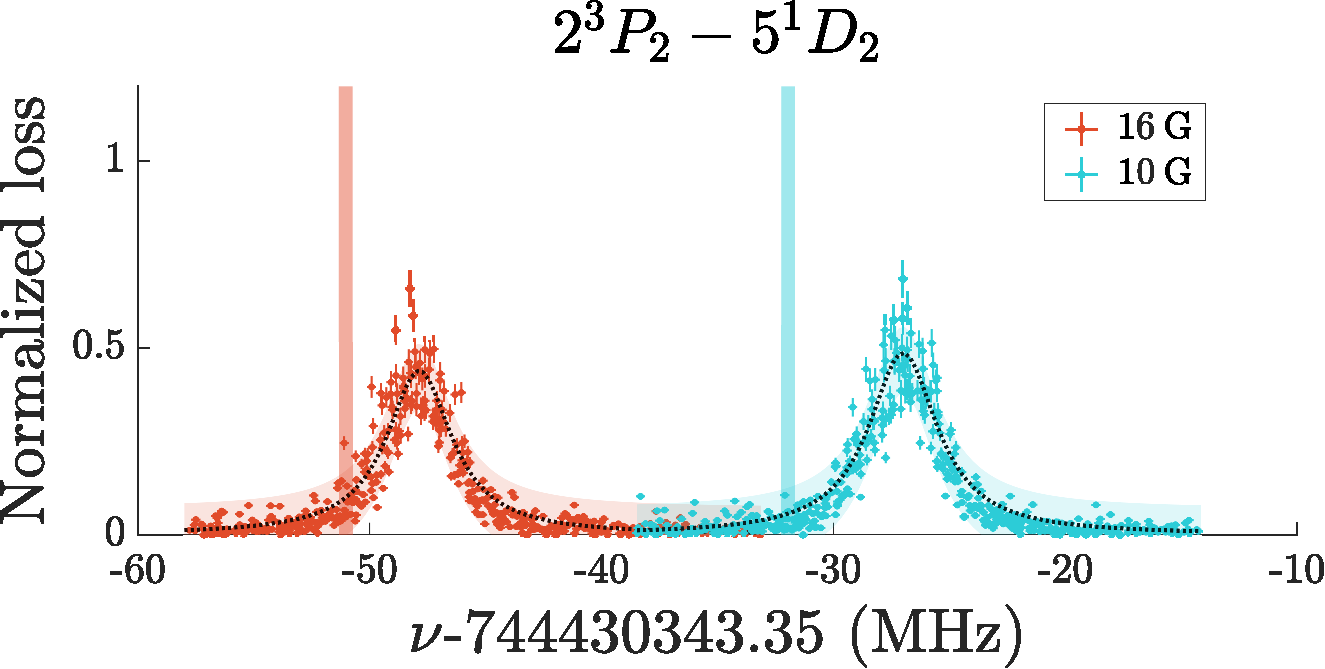
\includegraphics[width=0.66\textwidth]{fig/spectroscopy/ci-plot-51D2-eps-converted-to.pdf}
%     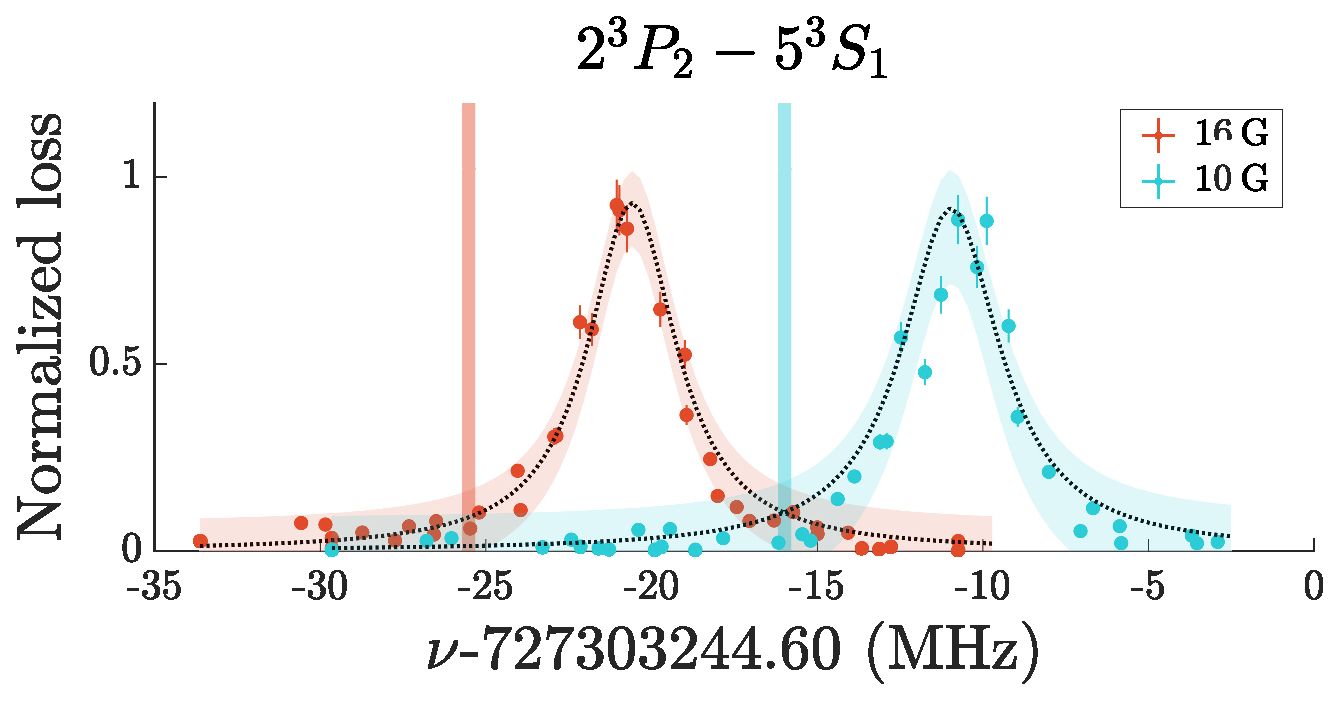
\includegraphics[width=0.66\textwidth]{fig/spectroscopy/ci-plot-53S1}
%     \caption{Line profile for the spin-forbidden $\PStateManifold_2 -  5^{1\!}D_2$ and the $2\triplet P_2 - 5\triplet S_1$ resonances, showing normalized atom number loss versus probe laser frequency $\nu$, as measured in an {16.8(1)}G (red) and {10.06(7)}G (blue) background field, with Lorentzian fits (black dotted line, with prediction confidence interval shaded).
% 	Error bars account for detector efficiency and calibration model uncertainty.
% 	For comparison, theoretical predictions (vertical bars) Zeeman shifted from the predicted zero-field value \cite{Drake07} according to the field calibration, whose uncertainty (shaded width) is dominated by background field measurements.}
%     \label{fig:simple_lines}
%   \end{figure}


% Laser
	

	We illuminated the atoms with the probe light (generated by the system described in section \ref{sec:spec_laser}) during the Doppler cooling stage, then measured the relative number loss as a function of frequency.
	For the $5\singlet D_2$ and $5\triplet S_1$ states, the exposure time was of order 100 ms.
	The exact duration differed for each line to obtain a good SNR without saturating the atom loss.
	The light was $\sigma^-$ polarized to drive transitions to the $m_J=1$ states of the upper levels.
	For the forbidden $5\singlet D_2$ transition the beam was focused on the atom cloud with a waist of approximately $100\mu$m and a peak intensity of order $5\times 10^3$ W/m$^2$.
	For all other measurements the beam was collimated with a peak intensity of order $ 5$ W/m$^2$.
	The Doppler cooling stage uses two magnetic field strengths and so measurements could be made with bias field strengths of {16.5(3)} and {10.2(3)} Gauss, which were calibrated independently by RF spectroscopy.
	For each field strength, the atom loss (with respect to calibration shots) versus probe laser frequency can be fitted by a Lorentzian lineshape to obtain the centre frequency and full-width at half-maximum (FWHM).
	Results of these fits are shown in Fig.
	\ref{fig:simple_lines}, after corrections for the AOM and vapor cell shifts (see the supplementary material of \cite{Thomas20} for details on the latter).
	{The transduction from photon scattering to atom loss via evaporative cooling is complicated and not linear.
	However, fits using a nonlinear function of the Lorentzian lineshape differed from the simple Lorentzian fit by substantially less than the statistical uncertainty.}

	After correcting for the linear Zeeman shift, the field-free transition frequencies are fixed with sub-MHz statistical uncertainty.
	This determines the $2\triplet P_2-5\singlet D_2$ and $2\triplet P_2-5\triplet S_1$ transition energies to be 3MHz and 5MHz larger, respectively, than the predictions presented in \cite{Drake07}.
	However, the absolute accuracy of these measurements is limited by the instrumentation.
	The results (Tab.	\ref{tab:results}) are consistent with current predictions \cite{Drake07} within $2\sigma$ after accounting for all systematic uncertainties (Tab.	\ref{tab:errors}).

\section{5$\triplet$D fine structure}

	Unlike the $5\singlet D_2$ and $5\triplet S_1$ levels, the $5\triplet D$ manifold splits into fine structure sublevels, leading to multiple absorption peaks and requiring a more involved analysis.
	For this measurement, the final quarter-wave plate in the insertion optics was rotated to give a combination of $\pi$ and $\sigma^-$ polarized light (in the atomic frame) as opposed to pure $\sigma^-$ light.
	This light drove transitions to the $5\triplet D_J, J\in\{1,2,3\}$ levels and obtained four peaks, as shown in Fig.	\ref{fig:combined_5D_lines}.
	The saturated peak near -300MHz (relative to the predicted $2\triplet P_2 - 5\triplet D_1$ interval) is in fact two peaks corresponding to the $5\triplet D_2(m_J=1)$ and $5\triplet D_3(m_J=2)$ states, which are separated by less than their linewidth. 
	This illustrates a shortcoming of the technique, namely the limited dynamic range.
	For measurements of single peaks this is not an issue as the total irradiated energy can be adjusted to obtain a good signal-to-noise ratio without completely depleting the BEC.
	In this case, however, there is a trade-off between keeping the small peaks above the noise floor and preventing the superposed peaks from saturating.
	This limitation could be eased with a larger initial condensate because the dynamic range is essentially limited by the atom loss, or with much larger magnetic field strengths which would ensure the lines are separated by much more than their linewidth.
	The other peaks correspond to transitions to the $5\triplet D_2(m_J=2)$, $5\triplet D_2(m_J=1)$, and $5\triplet D_1(m_J=1)$ states, which are used in the analysis described below.

	The Zeeman shift of the $J=2$ and $J=3$ levels is comparable to the interval between them, and so the mixing of levels means the correction is no longer proportional to $B$.
	Instead, the Zeeman shift can be corrected for by solving the eigenvalue optimization problem 
%
\begin{equation}
\textrm{min}_{E_{\textrm{fs}}} \sum_{J,m_J} \left(\nu_{{J,m_J}}^{\textrm{{pred}}}(E_{\textrm{fs}},B) - \nu_{{J,m_J,B}}^{\textrm{{obs}}}\right)^2,
\label{eqn:opt-problem}
\end{equation}
%
which minimizes the squared error between observed and predicted transition frequencies ($\nu^{\textrm{{obs}}}$ and $\nu^{{\textrm{pred}}}$ respectively), summed over all relevant $|J,m_J\rangle$ states and magnetic field strengths $B$.
	The optimized variable $E_{\textrm{fs}}=(E_1,E_2,E_3)$ is the bare fine-structure splitting of the $5\triplet D$ levels.
	In the argument below, the only assumption is the formalism of atomic structure theory and the data from the experiment.
	To determine the bare $5\triplet D$ transition energies from the data, consider the Hamiltonian
%
\begin{equation}
    \hat{H}(B) = \hat{H}_{\textrm{fs}} - B\hat{\mu}_z,
    \label{eqn:hamiltonian}
\end{equation}
%

\begin{figure}
	\centering
	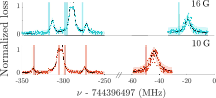
\includegraphics[width=\textwidth]{fig/spectroscopy/ci-plot-53D}
   \caption{Line profiles for the $\PStateManifold_2 -  5^{3\!}D$ transitions, shown as for Fig.
	\ref{fig:simple_lines}.
	The normalized loss is shown versus probe laser frequency for the two different field strengths with a common horizontal scale.
	Theory lines indicate predictions from \cite{Drake07} after applying the relevant Zeeman shift.
	N.B.	the scale break here and in Fig.	\ref{fig:fitting_3D} coincide.}
    \label{fig:combined_5D_lines}
\end{figure}

% \begin{figure}
%   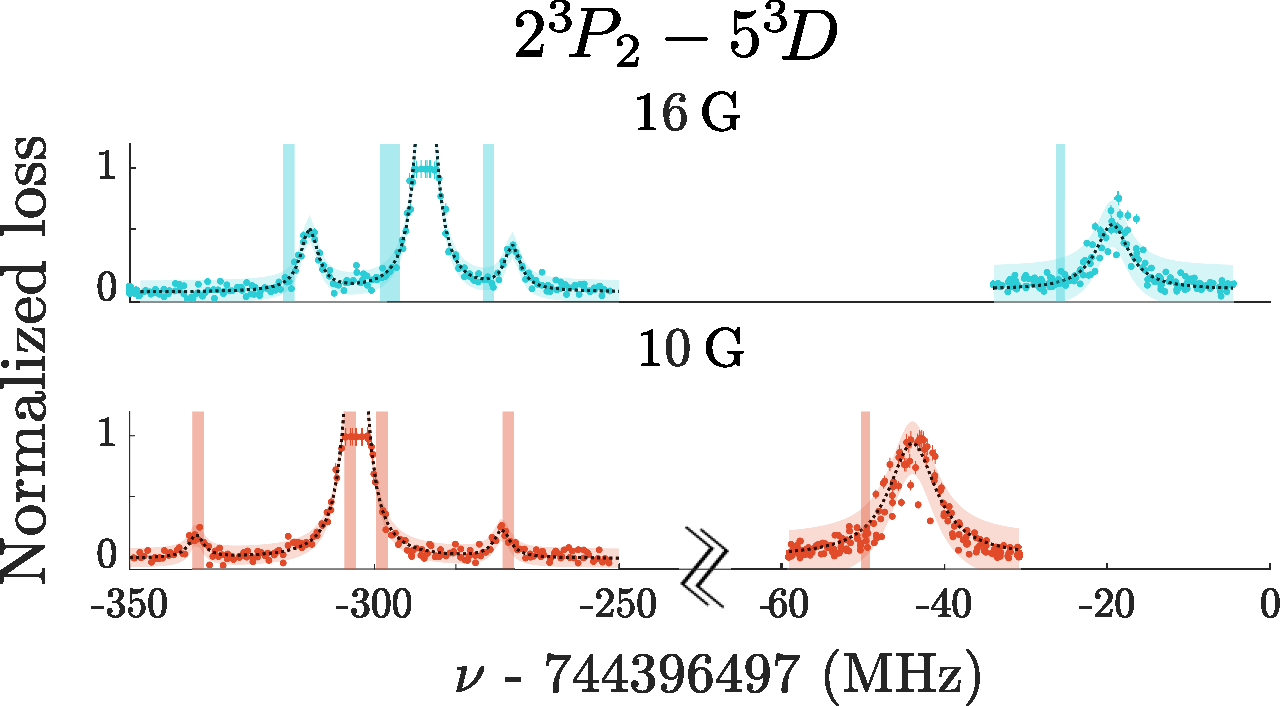
\includegraphics[width=0.5\textwidth]{fig/spectroscopy/ci-plot-53D-eps-converted-to.pdf}
%   \caption{Line profiles for the $\PStateManifold_2 -  5^{3\!}D$ transitions, shown as for Figs.
% 	\ref{fig:simple_lines}.
% 	The normalized loss is shown versus probe laser frequency for the two different field strengths with a common horizontal scale.
% 	Theory lines indicate predictions from \cite{Drake07} after applying the relevant Zeeman shift.
% 	N.B.	the scale break here and in Fig.	\ref{fig:fitting_3D} coincide.}
%   \label{fig:combined_5D_lines}
% \end{figure}

%
	\noindent where $\hat{\mu}_z = \mu_B(\hat{L}_z + g_s \hat{S}_z)/\hbar$ is the coupling of the orbital and spin angular momenta of the electron with a magnetic field of strength B pointing in the $z$-direction, $\mu_B$ is the Bohr magneton and $g_s$ is the electron spin $g$-factor.
		The fine structure Hamiltonian $\hat{H}_{\textrm{fs}}$ is diagonal in the $|LSJ m_J\rangle$ basis with eigenvalues $E_{\textrm{fs}}$,
	%
	\begin{equation}
	  \hat{H}_{\textrm{fs}}|LSJm_J\rangle = E_{\textrm{fs},LSJ}|LSJm_J\rangle,
	\end{equation}
	%
	which are degenerate for all $m_J$ with fixed $J$.
		The magnetic moment $\hat{\mu}_z$ couples states of different $J$, and is instead diagonal in the $|L m_L S m_S\rangle$ basis.
		In the $|LSJ m_J\rangle$ basis the matrix elements of $\hat{H}(B)$ are, with abbreviated notation,
	%
	\begin{equation}
	\begin{aligned}
	H_{J',J} =& \langle J'|\hat{H}|J \rangle\\
	  =& E_{\textrm{fs},J} - B \frac{\mu_B}{\hbar} \sum_{m_L} (2m_J - m_L)C_{J,'m_L}C_{J,m_L},\\
	\end{aligned}
	\end{equation}
	%
	where $C_{J,m_L} = \langle LSJ m_J|L m_L S m_S\rangle$ is shorthand for the Clebsch-Gordan coefficients.
		For $B>0$, the contribution of $\hat{\mu}_z$ breaks the degeneracy of $\hat{H}_{\textrm{fs}}$, giving rise to the Zeeman shift.
		
	%
	%
	\begin{figure}
	\centering
		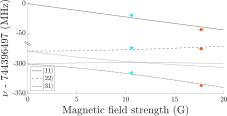
\includegraphics[width=0.9\textwidth]{fig/spectroscopy/fitting-lines}
		\caption{Determining the $5\triplet D$ fine-structure splitting.
		The values for the $|J,m_J\rangle=5\triplet D_J(m_J)$ levels (grey lines) at $B=0$ are fixed by solving the optimization problem (Eqn.
		\ref{eqn:opt-problem}), constrained by the fitted peak centres (filled circles).
		The saturated peaks are not used to constrain the levels and are not shown here. \com{}
		The corresponding frequencies predicted by the optimization method are shown in dotted lines.}
	    \label{fig:fitting_3D}
	\end{figure}

	The solution of Eqn.
	\ref{eqn:opt-problem} is illustrated in Fig.
	\ref{fig:fitting_3D}.
	By defining the energies $E_{\textrm{fs}}$ relative to the $2\triplet P_2(m_J=2)$ state,  the predicted transition frequencies can be read directly from the eigenvalues of $\hat{H}$ via $\nu_{J,m_J}^{\textrm{pred}}=E_{J,mJ}(B)/h$, where $h$ is Planck's constant.
	The observed frequencies $\nu_{J,m_J,B}^{\textrm{obs}}$ used in this procedure exclude the overlapping saturated peaks because their centre frequencies cannot be determined with satisfactory accuracy.
	The triple $E_{\textrm{fs}}$ which minimizes the cost function (Eqn.
	\ref{eqn:opt-problem}) corresponds to the $2\triplet P_2 - 5\triplet D_J$ intervals at $B=0$, as listed in Tab.
	\ref{tab:results}.
	Again, the difference in this determination of the field-free splitting is consistent within 2$\sigma$ predictions in \cite{Drake07} after accounting for systematic effects (Tab.
	\ref{tab:errors}).
	


% \usepackage{floatrow}



% \begin{figure}
% \floatbox[{\capbeside\thisfloatsetup{capbesideposition={left,top},capbesidewidth=4cm}}]{figure}[\FBwidth]
% {\caption{A test figure with its caption side by side}\label{fig:test}}
% {\includegraphics[width=5cm]{name}}
% \end{figure}

% \begin{figure}
% \floatbox[{\capbeside\thisfloatsetup{capbesideposition={right,top},capbesidewidth=4cm}}]{figure}[\FBwidth]
% {\caption{A test figure with its caption side by side}\label{fig:test}}
% {\includegraphics[width=5cm]{name}}
% \end{figure}




% \begin{figure}
% 	\begin{minipage}[t]{0.38\textwidth}
% 			\vspace{0pt}
% 			\caption{Determining the $5\triplet D$ fine-structure splitting.
% 	The values for the $|J,m_J\rangle=5\triplet D_J(m_J)$ levels (grey lines) at $B=0$ are fixed by solving the optimization problem (Eqn.
% 	\ref{eqn:opt-problem}), constrained by the fitted peak centres (filled circles).
% 	The saturated peaks are not used to constrain the levels, but are shown with hollow circles and the corresponding frequencies predicted by our method are shown in dotted lines.}
%     \label{fig:fitting_3D}
% 	\end{minipage}\hfill
% 	\begin{minipage}[t]{0.6\textwidth}
% 		\vspace{0pt}
% 		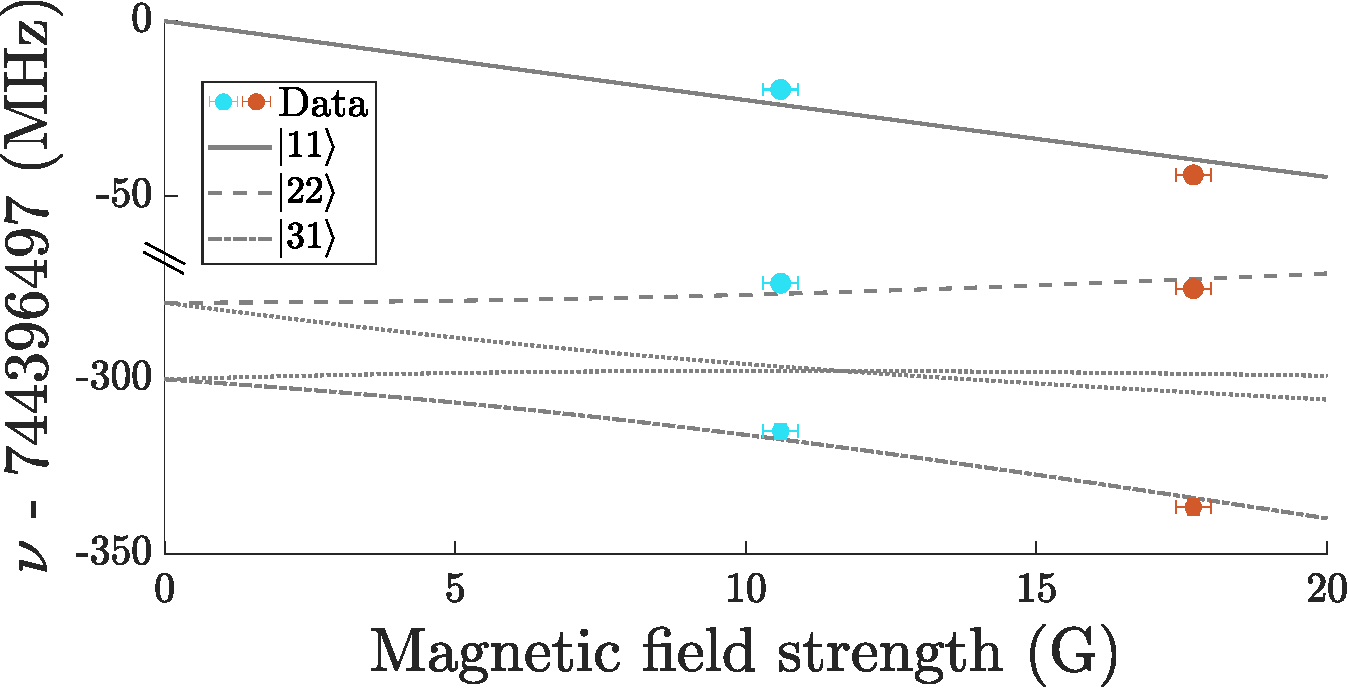
\includegraphics[width=\textwidth]{fig/spectroscopy/fitting-lines-eps-converted-to.pdf}
% 	\end{minipage}

% \end{figure}

% \begin{figure}
%     \centering
%     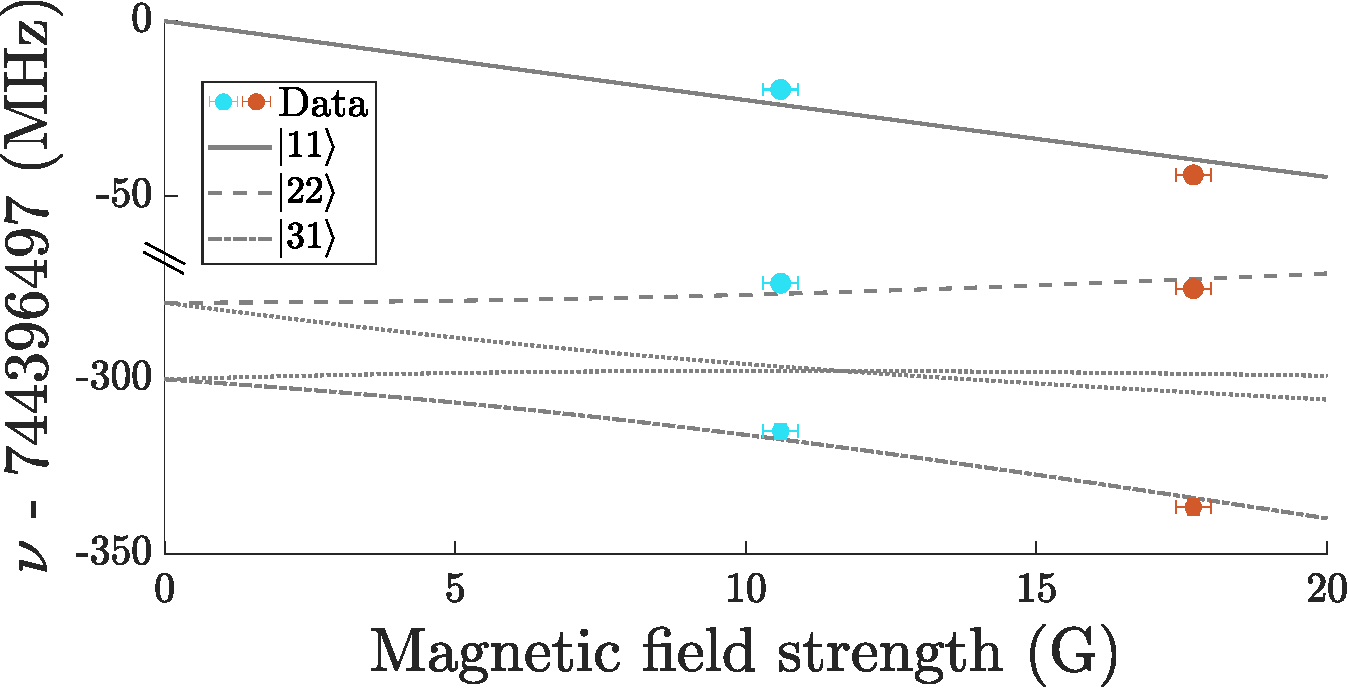
\includegraphics[width=0.48\textwidth]{fig/spectroscopy/fitting-lines-eps-converted-to.pdf}
%     \caption{Determining the $5\triplet D$ fine-structure splitting.
% 	The values for the $|J,m_J\rangle=5\triplet D_J(m_J)$ levels (grey lines) at $B=0$ are fixed by solving the optimization problem (Eqn.
% 	\ref{eqn:opt-problem}), constrained by the fitted peak centres (filled circles).
% 	The saturated peaks are not used to constrain the levels, but are shown with hollow circles and the corresponding frequencies predicted by our method are shown in dotted lines.}
%     \label{fig:fitting_3D}
% \end{figure}



\begin{table*}
\centering
  % \begin{tabular}{c c c c c c c c c c c}
  %     \hline\hline
  %     Transition                        & &  $f_\textrm{exp}$ & &  $f_\textrm{theory}$ & Ref.
		% &  $f_\textrm{exp}-f_\textrm{theory}$      & &  $\textrm{FWHM}_{\textrm{exp}}$  & &  $\textrm{FWHM}_{{\textrm{pred}}}$ \\
  %     \hline
  %       $2\triplet P_2 - 5^3\mathrm{S}_1$ & &  {727,303,248(3)} & &  727,303,244.6(4)   & \cite{Drake07} &  {3(3)}    & &  3.4(5)  & &  1.5\\ % A = 
  %       $2\triplet P_2 - 5^3\mathrm{D}_1$ & &  {744,396,496(7)} & &  744,396,511.1(7)   & \cite{Yerokhin20} &  {-16(7)}    & &  5.8(6)  & &  2.6\\
  %       $2\triplet P_2 - 5^3\mathrm{D}_2$ & &  {744,396,220(7)} & &  744,396,227.6(7)   & \cite{Yerokhin20} &  {-8(7)}    & &  4.2(5)  & &  2.6\\
  %       $2\triplet P_2 - 5^3\mathrm{D}_3$ & &  {744,396,194(7)} & &  744,396,208.3(7)   & \cite{Yerokhin20} &  {-14(7)}    & &  4.0(1)  & &  2.6\\
  %       $2\triplet P_2 - 5^1\mathrm{D}_2$ & &  {744,430,343(7)} & &  744,430,343.1(7)   & \cite{Yerokhin20} &  {0(7)}    & &  3.2(1)  & &  2.2\\  % 744430344
  %     \hline\hline
  %   \end{tabular}

    \begin{tabular}{c c c c c c c c c c c}
      \hline\hline
      Transition                        &  $f_\textrm{exp}$ &  $f_\textrm{theory}$ & Diff.
		  &  $\textrm{FWHM}_{\textrm{exp}}$  &  $\textrm{FWHM}_{{\textrm{pred}}}$ \\
      \hline
        $2\triplet P_2 - 5^3\mathrm{S}_1$ &  {727,303,248(3)} &   727,303,244.6(4)   &  {3(3)}      &  3.4(5)  &  1.5\\ % A = 
        $2\triplet P_2 - 5^3\mathrm{D}_1$ &  {744,396,496(7)} &   744,396,511.1(7)   &  {-16(7)}     &  5.8(6)  &  2.6\\
        $2\triplet P_2 - 5^3\mathrm{D}_2$ &  {744,396,220(7)} &   744,396,227.6(7)   &  {-8(7)}      &  4.2(5)  &  2.6\\
        $2\triplet P_2 - 5^3\mathrm{D}_3$ &  {744,396,194(7)} &   744,396,208.3(7)   &  {-14(7)}     &  4.0(1)  &  2.6\\
        $2\triplet P_2 - 5^1\mathrm{D}_2$ &  {744,430,343(7)} &   744,430,343.1(7)   &  {0(7)}      &  3.2(1)  &  2.2\\  % 744430344
      \hline\hline
    \end{tabular}
\caption{Summary of results for each transition.
	After correcting for the AOM and vapor cell shifts, the centre frequencies obtained from Lorentzian fits have statistical error at the $10\textrm{kHz}$ level.
	The field-free energies follow after correcting for Zeeman shifts, shown with theoretical predictions in the row below.
	The difference between our measurements and theoretical predictions is comparable with the experimental error.
	Observed full width at half maximum line widths (FWHM) of the Lorentzian fit to each line are shown in comparison to predicted linewidths as given in \cite{Drake07}.
	$f_\textrm{theory}$ for the $2\triplet P_2 - 5^3\mathrm{S}_1$ line comes from \cite{Drake07}, all others from \cite{Yerokhin20}
	All values are in MHz with uncertainty in the final digit in parentheses.}
  \label{tab:results}
\end{table*}

\section{Shifts, broadening, and errors}




% summarize results

	The results of these measurements are summarized in Tab.
	\ref{tab:results} and are consistent with theoretical predictions \cite{Morton06} within $2.1\sigma$ or less.
	The accuracy of these determinations of the field-free transition energies is limited by the absolute accuracy of the wavemeter.
	High Finesse specifies \cite{HighFinesseDoc} a 3$\sigma$ accuracy of 2MHz within 2nm of a calibration line (as in the transition to the $5\triplet S_1$ state), and 10MHz for all other lines measured.
	Because the wavemeter is used to lock the seed light for the doubler, the uncertainty is doubled in determinations of the absolute probe frequency.
	In Table \ref{tab:results} the corresponding 1$\sigma$ accuracy is shown in order to be consistent with other terms in our error budget, as displayed in Table \ref{tab:errors}.
	Note that this specification does not depend on the specific difference between the calibration and measured wavelengths, and may vary due to nonlinear dispersion of the wavemeter optics.
	Without an independent calibration this error cannot be rigorously constrained, which would be overcome with the instrumental improvements discussed below.
	As such, the 1-sigma errors determined in this way are presented with the caveat that they may be slightly underestimated.
	Still, all measured frequencies are consistent with predictions to within 2.1$\sigma$.
	Finally, the $5\triplet S_1$ transition line is 1.9nm away from the calibration line, and as such the 2MHz uncertainty may again be a slight underestimate.

\begin{table}
\centering
  \begin{tabular}{c c c}
      \hline\hline
          Source & Shift & Broadening  \\
      \hline
          Wavemeter ($5\triplet S_1$)& 0(1.3) & - \\
          Wavemeter (all other lines)& 0(6.7) & - \\
          Pump lock & - & 4$\times10^{-2}$ \\
          Pump AOM & - & 0.3 \\
          Probe lock & - & 0.3\\
          Probe AOM & -189 & 1$\times10^{-6}$\\
          Zeeman & Variable & Variable \\
          Recoil & - & 1.4$\times 10^{-3}$ \\ % assume angle accurate to 1deg
          Doppler & - & 2.7(4) \\
          Interference effects & 0.5 & - \\ 
          Cs cell & -1.9 & 0.4 \\
          \textbf{Total} ($5\triplet S_1$ level) & -190.9(1.7)+ZS& 2.2\\
          \textbf{Total} (all other levels) & -190.9(6.7)+ZS& 2.2\\
      \hline\hline
  \end{tabular}
\caption{Error budget for the determination of the peak centre frequencies.
	 The master laser for the pump beam is described in \cite{Shin16}.
	AOM stabilities were checked with an RF spectrum analyser.
	See \cite{Thomas20} for measurement of the Cesium cell shift and probe beam lock drift.
	The shift and uncertainty from the Zeeman shift (ZS) varies between the lines, so these contributions are omitted from the total.
	All values are in MHz.}
  \label{tab:errors}
  
\end{table}

	The linewidth of the pump and probe laser sources are 40kHz \cite{Shin16} and 200kHz \cite{Thomas20}, respectively.
	The laser lock error has a standard deviation of $100$kHz.
	The additional contribution from the pump and probe AOMs are 300kHz and 1Hz, respectively, as determined with an RF spectrum analyser.
	

{I obtained the magnetic field calibrations by measuring the number of atoms detected by the MCP-DLD after applying 300ms of RF radiation at variable frequencies (see Fig. \ref{fig:RF_spec}).
The number $n_\delta(\nu)$ of detections probes the population of trapped atoms $n_\text{T}(B)$ subject to a magnetic field strength $B$ through the relation $2 \mu_B B = h \nu$.
	
As shown in Fig.
	\ref{fig:RF_spec}, $n_\text{D}(B)$ follows a Bose-Einstein distribution with a chemical potential $g \mu_B B_0$, where $B_0$ is the bias in the magnetic field strength and $g\approx2$ is the g-factor of the $2\triplet S_1$ state.
	The Bose-Einstein fit provides a model for $n_\text{T}(B)$ and an estimate of the temperature of the cloud at each stage of the cooling process (and thus at each field strength).
	We can use the average temperature of $\sim130(20)\mu K$ to estimate  Doppler broadenings of 100(10) kHz and 2.6(3) MHz for the pump and probe transitions, respectively.

	Kinetic effects do not contribute any significant uncertainty in these frequency measurements, rather they just broaden the observed peaks.
	The pump light was applied by two counterpropagating beams, subtending angles of 15$^\circ$ and 195$^\circ$ relative to the direction of propagation of the probe beam.
	Photon absorption events contribute a recoil velocity of magnitude $\cos(15^\circ)\cdot\hbar k/m\approx6$mm/s, imparting a Doppler shift of order 1.4kHz.
	Atoms may absorb probe light after absorbing a photon from the pump beams, but not after decaying again, so the decay events do not contribute.
	Because there were two counterpropagating pump beams, the resulting contribution is a negligible broadening, especially in comparison with the thermal broadening.
	The 1-3 MHz difference between predicted and observed line widths is well accounted for by these broadening effects, mainly by Doppler broadening.
	\com{Is it worth including a Voigt fit to the profiles to extract homogenous broadening and natural linewidth? Would give lifetime measurement but not accurately enough to be very interesting.}

	The optical absorption profile near the 1083nm pump transition can be calculated by convolving $n_\text{T}(B)$ with Zeeman-shifted absorption profile of the 1083nm transition, which is a Lorentzian $\mathcal{L}_\text{abs}(f,B)$ with a 1.6 MHz FWHM \cite{Drake07}.
	The pumping rate at a given field strength is given by the convolution of $\mathcal{L}_\text{abs}(f,B)$ with the pump laser line $\mathcal{L}_\text{L}(f)$.
	Hence, the range of magnetic field strengths $B$ at which atoms were pumped to the $2\triplet P_2$ state were concentrated at field strengths of 10.2(3) G and 16.5(3) G for the two measurement stages.

	The Zeeman shift of the $2\triplet P_2 - 5L, L\neq D$ transitions is given by $\Delta E = \mu B (g_e m_e-g_g m_g)$, whose error is obtained by standard propagation of uncertainties.
	
	For the $5\triplet D$ states, the uncertainty in the iterative method described above follows from varying the magnetic field constraints within the range of experimental uncertainty ($0.3$G). }


	\begin{figure}
	\centering
  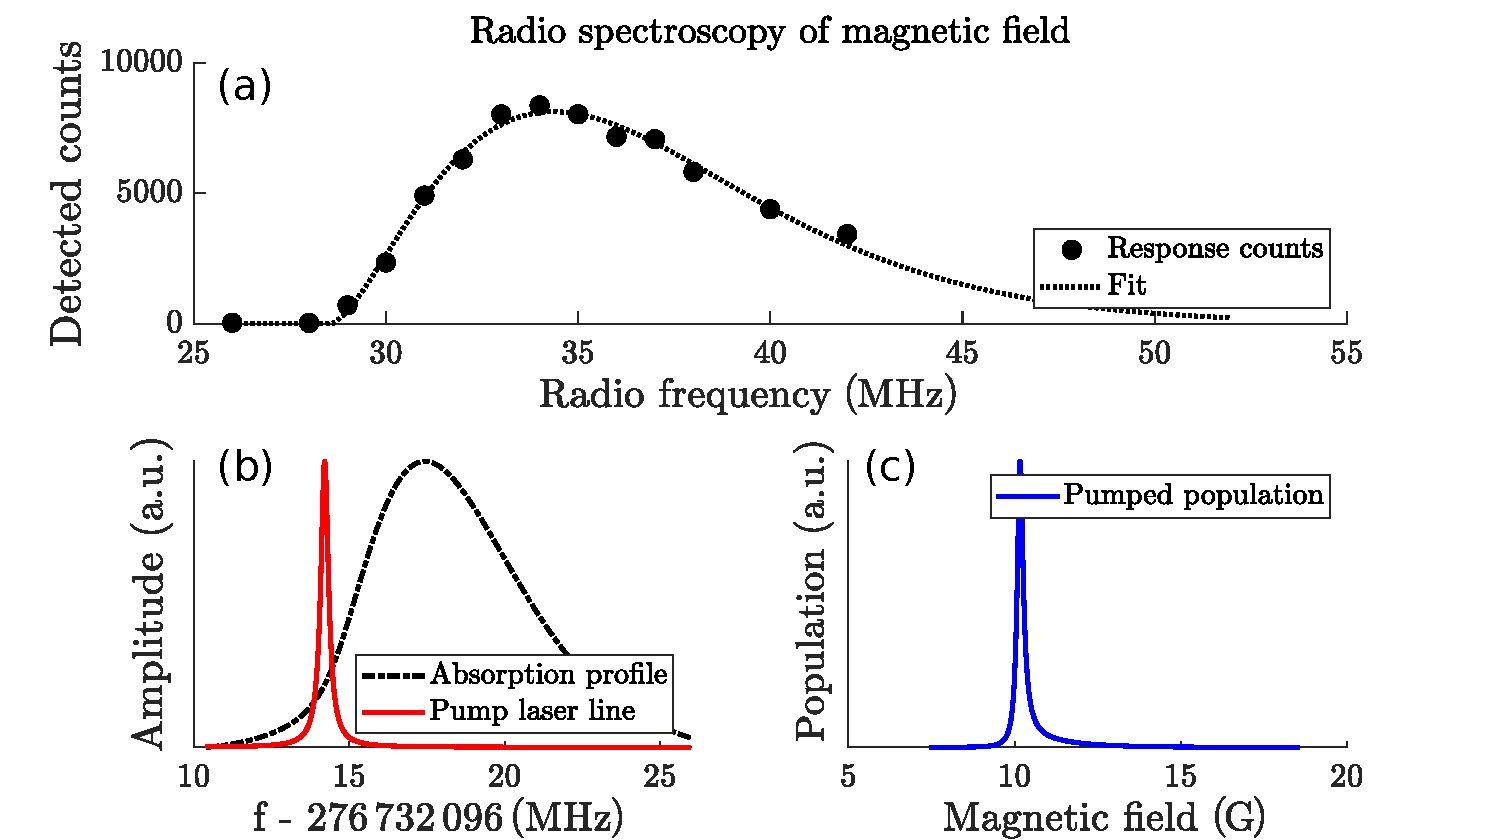
\includegraphics[width=\textwidth]{fig/spectroscopy/rf_spec_subfig-eps-converted-to.pdf}
  \caption{Determination of magnetic field for Zeeman shift correction.
	The number $n_\text{D}$ of atoms detected after probing the trap with 300ms of RF radiation is shown in (a) versus the frequency of the applied radiation.
	Each point is an average of three shots.
	A Bose-Einstein fit models the population density $n_\text{T}$ of the $2\triplet S_1$ state at a given field strength.
	In (b) the calculated absorption profile of the gas in the vicinity of the 1083nm pump transition is shown, along with the spectral profile of the pump laser.
	The pump laser selectively excites atoms with a certain Zeeman splitting, leading to a population of atoms in the $2\triplet P_2$ state (c) that is concentrated around a specific magnetic field strength.
	The resulting Zeeman broadening is dominated by the probe beam linewidth.}
  \label{fig:RF_spec}
\end{figure}


% \begin{figure}
% 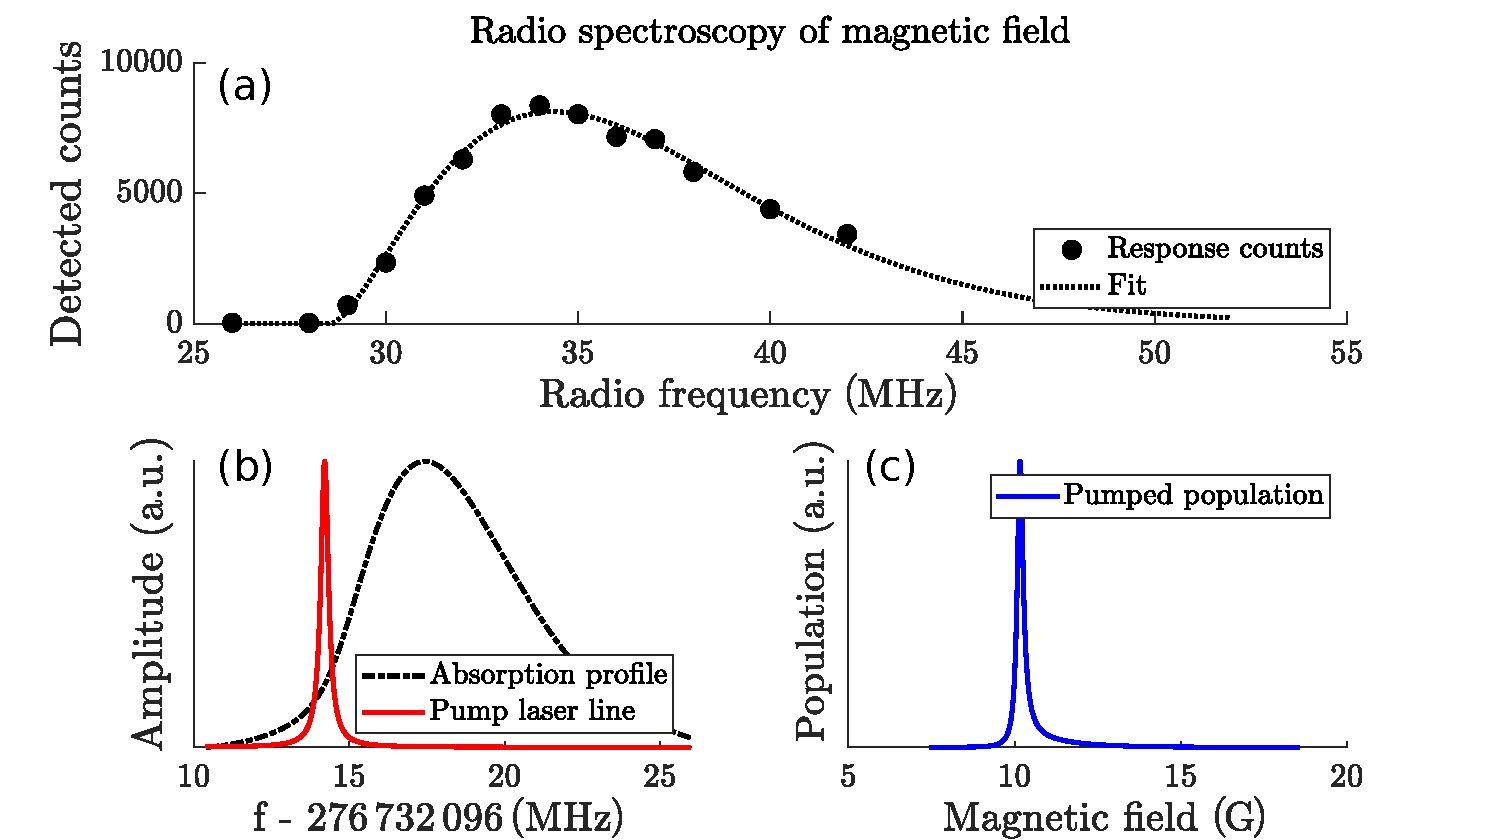
\includegraphics[width=0.5\textwidth]{fig/spectroscopy/rf_spec_subfig-eps-converted-to.pdf}
% \caption{Determination of magnetic field for Zeeman shift correction.
% 	The number $n_\text{D}$ of atoms detected after probing the trap with 300ms of RF radiation is shown in (a) versus the frequency of the applied radiation.
% 	Each point is an average of three shots.
% 	A Bose-Einstein fit models the population density $n_\text{T}$ of the $2\triplet S_1$ state at a given field strength.
% 	In (b) the calculated absorption profile of the gas in the vicinity of the 1083nm pump transition is shown, along with the spectral profile of the pump laser.
% 	The pump laser selectively excites atoms with a certain Zeeman splitting, leading to a population of atoms in the $2\triplet P_2$ state (c) that is concentrated around a specific magnetic field strength.
% 	The resulting Zeeman broadening is dominated by the probe beam linewidth.}
% \label{fig:RF_spec}
% \end{figure}

% The probe laser can only excite atoms pumped into the $2\triplet P_2$ state, which has a population distributed over a finite range of magnetic field strengths.
	% The peak of the response to the probe laser is given by the convolution of the probe laser spectrum and the density of pumped states over the magnetic field strengths.
	% We identify the 

% Finite temp in non-uniform field would lead to Zeeman broadening as well as a shift...
	% ungh run the trap sim?

	


\begin{figure}
  \begin{minipage}[t]{0.6\textwidth}
  \vspace{0pt}
  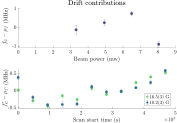
\includegraphics[width=\textwidth]{fig/spectroscopy/power-drift-combined}
  \end{minipage}\hfill
  \begin{minipage}[t]{0.38\textwidth}
  \vspace{0pt}
\caption{Top: Variation in fitted centre frequency for single scans across the $5\triplet D_1$ line versus applied laser power.
	The measurements at increasing beam power were not taken in chronological order Bottom: Variation in fit center frequency for the $2\triplet P_2 - 5\singlet D_2$ between scans.
	The value of the fitted peak centre $f_\textrm{c}$ is shown for each field strength, relative to the mean $\mu$ of all values for that field strength.}
\label{fig:power_drift_combined}
  \end{minipage}
\end{figure}

% \begin{figure}
% \includegraphics[width=0.48\textwidth]{fig/spectroscopy/power-drift-combined-eps-converted-to.pdf}
% \caption{Top: Variation in fitted centre frequency for single scans across the $5\triplet D_1$ line versus applied laser power.
% 	The measurements at increasing beam power were not taken in chronological order Bottom: Variation in fit center frequency for the $2\triplet P_2 - 5\singlet D_2$ between scans.
% 	The value of the fitted peak centre $f_\textrm{c}$ is shown for each field strength, relative to the mean $\mu$ of all values for that field strength.}
% \label{fig:power_drift_combined}
% \end{figure}

	Other precision measurements of transition frequencies have been shown to be subject to line pulling effects \cite{Marsman15,Marsman15PRA}.
	These effects arise in multilevel transitions because of interference between the laser-driven transition path and off-resonant driving through transitions with neighbouring intermediate states.
	The worst-case shift can be approximated by $w_{\text{pump}}^2/\Delta_{2P} + w_{\text{probe}}^2/\Delta_{5L}$ \cite{Marsman15,Marsman15PRA}, where the $w$ terms are the linewidths of the pump and probe transitions, and the $\Delta$ terms are the Zeeman splittings between the sublevels of the pump and target states.
	The largest estimate among all the reported transitions is 500kHz.
	While this uncertainty is dominated by other effects in our experiment, it may be important to understand them for improved measurements in the future.
	\com{I actually think this is bogus because we drove through (hyperfine) magnetic sublevels. For these, $\Delta\rightarrow 0$ at B=0, so the above expression would diverge, as oppsed to the case in Marsman \emph{et al} where they considered fine structure sublevels with $\delta>0$ at $B=0$. Without doing the calculations I suspect this rule of thumb doesn't actually apply to hyperfine levels but I'm not certain. Either way I will probably leave this in, as I'm unsure whether it's worth entering into that discussion.}

	There was no significant detectable contribution from the AC Stark effect.
	During measurements of the $5\triplet D_1$ transition with varying probe beam powers, the dependence of the centre frequency on the laser power was dominated by the drift in the wavemeter output, as shown in Fig.
	\ref{fig:power_drift_combined}.
	For the triplet-singlet transition, the increase in laser intensity is more than compensated for by the reduced dipole matrix element, and hence the same conclusion follows.
	



\section{Discussion}

	This chapter described multilevel laser absorption spectroscopy of excited state transitions in ultracold helium.
	The observations include the first observation (to my knowledge) of the forbidden $2\triplet P_2 - 5\singlet D_2$ transition.
	These measurements agree with current predictions within the error budget and suggest that the $93\sigma$ difference between previous measurements \cite{Martin60} and predictions \cite{Morton06} of the $\PStateManifold_2  -  \UpperS$ and $\PStateManifold_2  -  \UpperStateManifold$ intervals are due to an unkown systematic error \footnote{As a historical note on the advancement of experimental methods, Martin's measurements were made using a nitrogen-cooled helium discharge lamp fed through an in-vacuum prism onto photographic plates, on which the line separations were measured by hand with a ruler.}.
	This work offers five contributions to the NIST database of atomic spectral lines.

	The techniques described here are readily extensible to other opportunities in $^4$He structure measurements.
	For example, while there is an outstanding 7.4$\sigma$ disagreement between the predicted and observed singlet-triplet interval for the n=3 level in $^3$He \cite{Morton06,Derouard80}, the corresponding transition in $^4$He has never been directly measured.
	An indirect measurement in $^4$He could be made with the techniques described here by taking the difference betweeen the $2\triplet P_2 - 3\triplet D_2$ and $2\triplet P_2 - 3\singlet D_2$ transitions near 587.6nm and 587.4nm.
	While the latter transition is also spin-forbidden, it is predicted to be an order of magnitude stronger than the $2\triplet P_2 - 5\singlet D_2$ transition reported here \cite{Morton06}.

	{Further, energies of other $2L-nD$ transitions in $^4$He are a few MHz larger than predicted, apparently independent of $L$ \cite{Wienczek19,Yerokhin20}.
	The results here deviate from this trend, and invite independent verification.
	Further study of transitions between states from different shells to MHz precision or better, in particular the prospective study of the $2\triplet P - 3 D$ intervals, would also provide further clarification.}

	Simply exchanging the light source would suffice to make these measurements, but a definitive comparison with theory would require an improved frequency reference.
	For instance, the hypothetical $10/n^3$ MHz shift could be checked by a measurement of the $2~P-n~D$ transitions accurate to sub-MHz precision.
	The associated theoretical uncertainties are about this size, dominated by the 700 kHz uncertainty in the lower state \cite{Pachucki17,Wienczek19}.
	As the $\alpha^7$ terms could improve the theoretical accuracy to as little as 10kHz \cite{Pachucki17}, this more challenging precision appears to be a more appropriate budget, and readily achievable with current methods.
	Reference-locked optical frequency combs can readily achieve kHz accuracy or better \cite{Luo15,Rengelink18}.
	Magnetic field strengths can be determined by RF spectroscopy with sub-kHz accuracy and so would not present a serious limitation.
	Improving the AOM frequency stability would provide sufficient accuracy to account for laser-induced stark shifts, likely leaving systematic drifts as the dominant source of error.

	Extending these methods to direct measurements on $^3$He would also permit isotope shift measurements from forbidden excited-state transitions in $\triplet$He.
	Theoretical calculations of isotope shifts are already accurate to the sub-kHz level, so such measurements would be even more demanding than the prospects above.
	Existing demonstrations of comparable accuracy \cite{Rengelink18} show such measurements are worthy challenges whose completion can access nuclear structure information at the femtometre scale via optical atomic spectroscopy.


\vfill

\begin{flushright}
\emph{
``Immediately you would like to know where this \\
number for a coupling comes from: is it related to pi\\
or perhaps to the base of natural logarithms? \\
Nobody knows.\\
It's one of the greatest damn mysteries of physics: a magic number \\
that comes to us with no understanding by man. You might say \\
the ``hand of God" wrote that number, and ``we don't know how\\
He pushed his pencil." We know what kind of a dance to\\
do experimentally to measure this number very accurately,\\
but we don't know what kind of dance to do on the computer\\
to make this number come out, without putting it in secretly!"}\\
- Richard P.
Feynman \footnote{\emph{QED: The Strange Theory of Light and Matter}.
	Princeton University Press.	p.	129.	(1985)}
\end{flushright}



% * Dipole operator -> Clebsch-Gordan again
% % Fermi's golden rule: $\Gamma_{ij} = \braket{i, H_{dip}, j}/\hbar$ ?

% This comes from the atom in an oscillating electric field.
	% The Hamiltonian is
% % $$
% % \hat{H} = \hat{H}_{\alpha} + \hat{H}_{\omega} + H_{int}\\
% 		% & H_{nLm_lSm_s} + \frac{\hat{n_\gamma}+1}/{2}\hbar\omega_\gamma ...\\
% 				% + \int H(\alpha,\omega) d\omega
% % $$
% where $\alpha$ and $\omega$ denote the Hilbert spaces of the atom and of the bosonic field, respectively, and $H_{\int}$ is the interaction term.
	% In the plane wave picture, we can think of the electromagnetic field, with modes $\omega$, then a \emph{coherent} field has several connotations and implications.
	 

% Classically, we can also describe the electromagnetic field as a vector field $E\times X$ with $E(x): (x,y,z,t) \rightarrow \mathcal{S(x)}$, where $S(x)$ is the Stokes vector at each point.

% \end{itemize}

% 	This chapter describes two measurement campaigns of electronic transition energies in Helium.
	% First, I recount the method and used to measure the energy splittings between the $\PStateManifold_2$ state and a collection of states in the $n=5$ manifold, including the first observation of a transition between the $2\triplet P$ and $5\singlet D$ manifolds in Helium.
	% Second, I describe two methods used to measure the energy and the transition lifetime of the forbidden $2\triplet S_2\rightarrow 3\triplet S_1$ transition, the weakest electronic transition observed in a neutral atom to date, previously considered too weak to be measured\cite{Lach01}.
	

% 	The work described in this chapter provided the basis for the following publications:

% 	\begin{itemize}
% 		\item K.F.Thomas, J.A.Ross, B.M.Henson, D.K.Shin, K.G.H.Baldwin, S.S.Hodgman, and A.G.Truscott, Direct Measurement of the Forbidden $2\triplet S_1\rightarrow 3\triplet S_1$ Atomic Transition in Helium, \emph{Journal} \textbf{issue}(2020), \href{<https://arxiv.org/abs/2002.04811>}{<arXiv>}
% 		\item J.A.Ross,  K.F.Thomas,  B.M.Henson,  D.Cocks, S.S.Hodgman,  K.G.H.Baldwin,  and  A.G.Truscott, Measurement of spin-forbidden excited-state transitions in metastable helium, \emph{Journal}, \textbf{issue} (2020) 
% 	\end{itemize}
% 	% Spec paper
% 	% forbidden paper

% 	\newpage

% \section{Measurement of five $2\triplet  P_2\rightarrow 5L$ transition energies}\label{sec:he-trans}

% 	Some of the $\PStateManifold_2\rightarrow5_D$ transitions were observed by Martin in 1960\cite{Martin60}, but his measurements are in stark disagreement with present predictions\cite{Wiese09} by about 13 GHz.
	% Further, in the NIST database, the transition energies to the $5\triplet D$ states are all identical\.
	% Indeed, in Martin's original paper, he only quotes measurements from $\PStateManifold$ to the $5D$ level in general, indicating that his equipment did not have the resolving power to distinguish the fine structure of the $5\triplet D$ state.
	% Martin was also unable to distinguish transitions to the $5\singlet D$ level, probably due to its proximity to the $5\triplet D$ lines .
	% The contents of this chapter are complementary to the following publications:

% \subsection{Tests of fundamental physics with helium spectroscopy}

% 	Quantum electrodynamics (QED) describes the interaction of light and matter.
	% It is the most accurate quantitative physical theory to date.
	% The state of the art of experimental atomic spectroscopy is sufficient to match theoretical uncertainties in table-scale experiments, signalling an era in which atomic physics laboratories can contribute to tests of fundamental physics.
	% Atomic structure predictions are made using the theory of QED and assuming the CODATA values of the fundamental constants.
	% With the present accuracy of theory and experiment, it is possible to back-calculate from observed data and constrain fundamental constants.
	% Schwartz identified opportunity to determine the fine structure constant in Helium in 1964, noting that the $\PStateManifold$ fine structure intervals are subject to strong QED effects, but have lifetimes about an order of magnitude larger than the same states in Hydrogen.
	

% 	The ongoing theoretical campaign \cite{Pachucki15,Pachucki17,Pachucki11,Pachucki10,Morton12,Morton06,Patkos16,Patkos17} has reached sufficient accuracy to obtain a $4\sigma$ discrepancy for the squared charge radii difference between Helium-3 and Helium-4 obtained from the $\MetastableState \rightarrow \PStateManifold$ and the $\MetastableState\rightarrow {2\singlet S_{0}}$ transitions\cite{Pachucki15}.
	

% 	A comprehensive tabulation of Helium levels and transition rates was compiled by Wiese and Fuhr in 2009 \cite{Wiese09}, based on the extensive work by Pachucki, Yerokhin, Morton, Drake, and collaborators.
	% These calculations were recently verified by Zhang et al \cite{Zhang15}.
	% Predictions are made using the theory of QED and assuming the CODATA values of the fundamental constants.
	% With the present accuracy of theory and experiment, it is possible to back-calculate from observed data and constrain fundamental constants.

% 	The theoretical campaign \cite{Pachucki15,Pachucki17,Pachucki11,Pachucki10,Morton12,Morton06,Patkos16,Patkos17}, has reached order $\alpha^6m^2/M$ in both singlet and triplet states states\cite{Patkos16,Patkos17}.
	% Efforts are ongoing to compute the $\alpha^7$ contributions expected to allow determination of the Helium nuclear charge radius accurate to 1\%\cite{Pachucki17}.
	% Already, there is sufficient accuracy to obtain a $4\sigma$ discrepancy between squared charge radii difference between Helium-3 and Helium-4 obtained from the $\MetastableState \rightarrow \PStateManifold$ and the the $\MetastableState\rightarrow {2\singlet S_{0}}$ transitions in each, namely $\delta r^2 = 1.069(3)~\textrm{fm}^2$ and $\delta r^2 = 1.061(3)~\textrm{fm}^2$ for the former and $\delta r^2 = 1.027(11)~\textrm{fm}^2$ for the latter\cite{Pachucki15}.
	% With improved calculations of $\PStateManifold$ splitting to 1.7kHz\cite{Pachucki17}, experimental precision is now the limiting factor in determining the isotope shift.
	

% 	Cancio Pastor \textit{et al.} used Helium spectroscopy to make the then-most accurate Lamb shift measurement in any atomic system\cite{Pastor04}.
	% Six years later, Smiciklas \textit{et al.} measured the $\PStateManifold$ fine structure splitting to sub-kilohertz precision, determining fine structure constant to 5ppb\cite{Smiciklas10}.
	% Measurement of the $2^3P-2^3S$ spacing to within 1.4kHz would determine the nuclear charge radius to below 0.1\%, better than expected from the muonic helium Lamb shift\cite{Wienczek19}.
	 

% 	Recently Kato \emph{et al} refined measurements of the $2\triplet  P_2\rightarrow2\triplet  P_1$ to 25Hz accuracy, which can constrain $\alpha$ to less than one ppb in conjunction with similarly accurate measurement of the $2\triplet  P_1\rightarrow2\triplet  P_0$ transition and QED corrections of order $\alpha^7$ \cite{Kato18}.
	% Ongoing efforts \cite{Pachucki17} to obtain these corrections will also allow determination of absolute nuclear charge radii accurate to better than 1\%, complementary to ongoing investigation of the proton radius puzzle.

% 	Curiously, measured transition energies from the $n=2$ manifold to the 3D levels are about 1MHz larger than predicted.
	% Assuming the usual $1/n^3$ scaling of QED effects, such an anomaly would imply a deviation of $10/n^3$ MHz in ionization energy for an arbitrary state, motivating further study of transitions between states from different shells \cite{Wienczek19}.
	% In this work, we measure five transitions from the $2^3P_2$ state to the $n=5$ level, improving on the precision of past measurements\cite{Martin60} by order of magnitude.
	% We resolve lines from the $\PStateManifold_2$ to the $\UpperSingletStates$ states individually for the first time.
	% We make the first observation of the spin-forbidden $2^3P_2\rightarrow5^1D_2$ transition in Helium.
	% Future measurements with greater precision could assist efforts to resolve a 7.5$\sigma$ disagreement between the predicted and observed $n=3$ singlet-triplet splitting\cite{Morton06}.

% 	\begin{figure}[b]
% 	    \centering
% 	    \includegraphics[width=\textwidth]{fig/Spectroscopy/level_diagram_tight_latex.eps}
% 	    \caption{A level diagram for the helium atom.
	% The transitions measured in this work (blue), are driven by a tunable laser referred to in text as the 'probe'.
	% The cooling transition (red) is referred to as 'pump' throughout the paper and populates the lower state of the target transitions.
	 % The doubly forbidden $1\singlet S_0\rightarrow2\triplet  S_1$ transition is excited in a high voltage discharge cell.
	% Transitions between the singlet and triplet manifolds (left and right of dotted line) are forbidden in the dipole approximation.
	% The level splittings are not to scale.}
% 	    \label{fig:lvl_diag}
% 	\end{figure}

% \subsection{Detection scheme}\label{ssec:spec-detection}
% \begin{itemize}
% 	\item Setup - alignment
% 	\item Procedure
% 	\item Mechanism
% 	\item Calibrations
% 	\item Analysis
% \end{itemize}

% \subsubsection{Procedure}
% 	We use a micrometer translation mount on the final lens to align the beam on the Helium sample.
	% We locate the transitions approximately by using the maximum available laser power at the predicted frequency, and then reducing the power and adjusting the frequency set point until the signal no longer saturates at the peak.
	% We then scan the set point of the laser across the transition to obtain the transition signal.
% 	The beam was initially aligned by tuning the probe beam to the predicted value of the 53S1 transition and operating with the maximum available power.
	% Although the uncertainy in wavemeter accuracy was larger than the transition linewidth, by operating well above the saturation intensity, the transition was broaded by tens of MHz and so the WM error was less significant.
	% When scanning the beam pointing across the expected target region, approximate alignment was signaled by a dramatic loss of atom number.
	% When the signal saturated, the power was lowered until the signal was just above the noise floor, and then scanning resumed.
	% This process iterated a few times until the maximum attainable signal was below saturation - that is, when for fixed power one could not completely destroy the trap.
	% Notice there are three kinds of saturation here: Atomic population saturation, detector saturation, and signal saturation when you run out of atoms.
	% perhaps the term `dynamic range' would be more suited to the latter\ldots{} Something to think about.

% 	During the calibration shots, we also block the beam with a mirror mounted on an automatic translation mount.
	% The profile and polarization of the beam are determined with lenses and waveplates prior to vacuum entry.
	% The measurement sequence consists of measurement shots with each of the two magnetic field strengths followed by calibration shots, wherein the laser beam is blocked and switched off.
	% We calibrate the wavemeter before each transition measurement.
	% Analysis of the wavemeter stability suggests that calibration drift is not a significant source of error, as discussed in the supplementary materials.

% 	The method therefore consists of alternating measurement trials with control trials, wherein the laser beam is blocked before the fibre coupler with a flipper mirror.
	% At the moment I use an interpolation, but I might want to try using a model-based estimate of the atom number.
	% Either way, there is going to be some error in the number estimation.
	% It's probably small.
	% The difference between the interpolated, unperturbed atom number and the detected number in the measurement trials is affected by the quantum efficiency and the introduced uncertainty in atom number.

% 	The polarization of the light was fixed with the waveplates before the chamber.
	% Can you tell handedness just by relative angle of waveplates? We hypothesized that the initial state of the atoms during the cooling phase was in the m=2 state, as the optics are configured to drive with a sigma+ beam during the in-trap cooling stage.
	% I verified this by driving with plane-polarized light (in the atom frame - put some trap sim in to show where the field points), which is a linear combination of sigma+ and sigma- light.
	% If there were atoms in initial states other than the m=2, then when driving to the 53S1 state, one would observe multiple peaks.
	% Instead, only one peak was observed, which vanished when the probe beam was set to sigma+ light.
	% (I think check the data).

% 	The measurements are taken at two different background field strengths.
	% Therefore the detuning from cooling resonance is X and Y MHz in each stage, respectively.
	% These values were calibrated independently by an RF spectroscopy technique.
	% This allows empirical extrapolation to the field-free transition energy by correcting for the calculated Zeeman shift of the centre frequency of each measured line.


% % Peak intensity is ~ total power x 1e3 /m^2 for large beam
% \begin{table}
% \begin{tabular}{|c|c|c|c|c|}
% \hline
% Line & Beam waist (cm) & Beam power (mW) &  Peak intensity (W/m$^2$) & Exposure time (ms)\\
% \hline
% $5\triplet S_1$  & 4.1 &  2.73(1) & 3.1(2) & 100 \\
% $5\triplet D_1$  & 4.1 &  4.5(1) & 5.2(1) & 150\\
% $5\triplet D_2,3$& 4.1 &  8.6(1) & 9.9(1) & 250  \\
% $5\singlet D_2$  & 0.1 &  10(2) & 6.3E3 & 100 \\
% \end{tabular}
% \label{tab:spec-beamparams}
% \caption{Probe beam parameters}
% \end{table}
% \begin{table}
% \begin{tabular}{|c|c|c|c|c|}
% \hline
% Stage & Beam power & AOM detuning & Peak intensity & Transition detuning\\
% \hline
% \end{tabular}
% \label{tab:spec-pumpparams}
% \caption{Pump beam parameters}
% \end{table}

% \subsubsection{Data acquisition}
% 	\com{This probably goes in the Intro/BEC machine part}

% 	Following the laser interrogation, the remaining atoms are gradually outcoupled from the trap with a pulsed atom laser.
	% At the beginning of each shot, the LabView control interface writes a line to the log file with the parameters \verb|timestamp, laser_setpt, shot_type| where \verb|shot_type| is either \verb|stage_1|, \verb|stage_2|, or \verb|calibration|.
	% When importing the data into the processing scripts, the 

% 	 As the laser set point is fixed for sets of three shots (one per field setting), 


% \subsubsection{Mechanism of action}
% 	
% 	To drive the transitions from the 23P2 state to the states in the n=5 manifold, I use the probe beam to disturb the near-resonant optical molasses cooling stage of the experiment.
	% This follows the MOT loading and precedes evaporative cooling, and operates with XYZ beam parameters for XXX ms, and then with ABC beam parameters for YYY ms.
	% I calculate that during these stages, the excited-state population is ZZZ per cent, which are then susceptible to scattering photons from the probe beam.

% 	I used the evaporative cooling sequence as a transducer between scattering-induced heating of the cloud and the final condensed number.
	% I will present a quantitative sketch of the mechanism below, but one can also take a heuristic understanding from the following argument:

% 	The evaporative cooling we use to achieve Bose-Einstein condensation has stringent tolerances on initial phase space density, which increases with number and at lower temperatures.
	% Tuning a radio chirp to the spin-flip transition from a trapped to an untrapped state and sweeping down to lower energies, higher-energy atoms are removed, the cloud rethermalizes at a lower temperature, and the phase space density increases.
	% Higher-energy atoms spend time further from the centre of a harmonic magnetic trap.
	% So, scattering photons from the probe beam heat the cloud, leading widening the velocity distribution, which drives more of the atoms into resonance with the radio chirp.
	% The final temperature is determined by the endpoint of the radio chirp.
	% Resonance with the probe light manifests as a signal in a reduction of the final population of the condensate.

% 	As I said, an essential part of our BEC production is an optical cooling and spin-polarizing stage which precedes the loading of our magnetic trap.
	% This ensures a nice large atom number and low temperature.
	% This give us a nice big phase space density, a dimensionless number which compares the length scale of quantum interference, the de Broglie wavelength, with the interparticle spacing given by the particle density n.~So, disturbances to this initial condition by atom loss or heating will reduce the phase space density input to the evaporation stage.
	% The Bose-Einstein condensation threshold occurs when the phase space density crosses about 2 - for comparison, atmosphere has a phase space density about one ten millionth of that.
	% One can therefore think of the RF evaporation as a phase space amplifier in the following way:

% 	Evaporative cooling works by creating a resonance between trapped and untrapped magnetic states of atoms with a specific Zeeman splitting by exposing the cloud to radio frequency radiation.
	% Energetic atoms travel up the magnetic field gradient, shown by the thickness of the purple lines, to the ellipsoidal shell defined by a fixed field strength at which the atoms resonate with the radio waves.
	% The atoms are then transferred into free states and leave the trap, taking with an amount of energy greater than the ensemble average.
	% This basically cuts out the upper tail of the Maxwell-Boltzmann distribution, driving down the atom number, but also the temperature once the cloud rethermalizes.
	% If you get this right, you continuously increase the phase space density by making the cloud cooler and smaller, until you get to BEC.
	% The endpoint of the RF chirp fixes an upper bound to the energy of the trapped atoms, and hence a temperature.
	% Then the phase space density can be estimated by counting the number of atoms you have left.
	% We measure this atom number using Helium's unique detectability - by applying broadband radio pulses to the trap we free about 0.5\% of the atoms at a time, creating a series of pulses of coherent matter waves, known as an atom laser.
	% This resolves on our detector as a series of discrete particle detection events, which we sum up with an abacus.
	% So by controlling our independent variable, the applied laser frequency, we have a gain mechanism that allows us to measure the dependent variable, which is the phase space density reduction by resonant scattering of photons from the probe beam.

% \subsubsection{Calibration measurements}

% 	After the probe is applied during the optical molasses cooling, we use a standard forced evaporative cooling procedure.
	% At the end of the sequence the atoms are in the metastable $2^3S_1$ state which exhibits a 19.8eV ground state separation.
	% This internal energy enables single-atom detection by a multi-channel plate and delay-line detector stack with an efficiency of 8 per cent\cite{Manning10} to determine the atom number loss.
	% We use a pulsed atom laser \cite{Manning10,Henson18} to transfer atoms to the untrapped state and avoid detector saturation.


% 	A translation mount on the final lens gives us micrometer precision in the placement of the focal point on the beam, which we use to align the beam on the trap, threading a ten micron needle in the dark 20 micro-radian accuracy.


% 	\begin{table}
% 	\label{tab:aom_calibration}
% 	\begin{tabular}{|c|c|c|c|}
% 		\hline
% 		RF centre frequency & Calibrated field strength (G) & AOM frequency (MHz) & Detuning (MHz) \\
% 		\hline
% 		XXX & 18 & 138 & 0.5\\
% 		XXX & 11 & 133.6 & 2\\
% 		\hline
% 	\end{tabular}
% 	\end{table}
% 	AO offsets 138MHz and 133.6MHz ?
% 	cooling transition is split 25.55 MHz, and 16.002 in stage 2
% 	Therefore the beams are (ish) detuned 0.5 and 2MHz respectively

% \subsubsection{Analysis}
% 	In this section I describe the data processing method used for the peaks, using the $5\singlet D_2$ line as an example.

% \subsection{Findings}\label{ssec:spec-findings}

% \subsubsection{Results}

% 	\begin{figure*}
% 	  % \includegraphics[width=\textwidth]{fig/Spectroscopy/pub_lines_j1.eps}
% 	  \caption{Measured line profiles for the $\PStateManifold_2\rightarrow 5\triplet  S_1$ (left) and   $\PStateManifold_2\rightarrow 5\triplet  D_1$ (right) transitions, with Lorentzian fits.
	% On the horizontal axis is the probe laser frequency $\nu$, relative to the theoretical prediction for the magnetic field-free splitting.
	% The vertical axis is the response as measured by atom number loss relative to the calibration shots.
	% Theoretical predictions (vertical bars) are Zeeman shifted from the zero-field value according to the field calibration, with uncertainty (horizontal bars) dominated by uncertainty in background field strength.
	% Lines obtained by measuring against an 18G and 11G background field are shown in red and blue, respectively.
	% }
% 	  \label{fig:simple_lines}
% 	\end{figure*}


% \subsection{Determination of transition energies}\label{ssec:spec-processing}


% \begin{figure}
% \includegraphics[width=\textwidth]{fig/spectroscopy/calib_model_51D2.eps}
% \label{}
% \caption{}
% \end{figure}

% \begin{figure}
% \includegraphics[width=\textwidth]{fig/spectroscopy/auto_peak_detect_51D2.eps}
% \label{}
% \caption{}
% \end{figure}

% \begin{figure}
% \includegraphics[width=\textwidth]{fig/spectroscopy/probe_set_err_51D2.eps}
% \label{}
% \caption{}
% \end{figure}

% \begin{figure}
% \includegraphics[width=\textwidth]{fig/spectroscopy/fitting_peaks_51D2.eps}
% \label{}
% \caption{}
% \end{figure}

% 	We empirically extrapolate to the field-free transition energy by correcting for the Zeeman shift in the observed lines.
	% The exposure time and intensity varied among measurements to avoid saturation.
	

% 	The table below displays the results of the measurements, including predicted linewidths.
	% In the case of the 23S1-33S1, the measured Einstein A coefficient is also listed.
	% These measurements are accurate to a few hundred parts per billion, and their accuracy is limited by the absolute accuracy of the wavemeter we used as a reference for the laser lock.
	% Within the accuracy stated by the manufacturer, these results are consistent with the predictions of QED.
	% Of the six lines measured, three have been resolved individually for the first time, and two have not been recorded elsewhere.
	% The centre frequencies are obtained by fitting Lorentzian profiles to the atom loss spectra.
	% Have a look at residuals; what are the expected broadening effects? What are the expected systematic errors? Error budget goes here also.
		

% 	Ah.
	% The CG madness is only needed for the triplet D states.
	% The singlet D and the triplet S have zero total angular momentum for the spin and orbital dof, respectively, so the basis is trivial and in these cases, we can use the linear extrapolation method with no worries.
	% What about the 2 3P2? Oh - I missed a point, which is the presence of other nearby levels.
	% For the singlet D, that's done, it's unique, as S=0.
	% And for the triplet S, also, as L=0.
	%  Not so for the 2 3P2.
	% But they're several GHz away so that shouldn't be a problem at all.
	% Well, then that's cleared up! Great.
	% Now to write this nonsense up.
	% Start concise in the paper, then we can expand it here.
	% later.

% % A and Sum A from \cite{Drake07}
% % Triplet D: 8.3444E+02 1.3929E+07
% % 5 3S1 line 2.4738E+06 sum 9.2072E+06
% % 5 3DJ sum 1.6412E+07
% % 	Lines
% % 	J=1 3.2224E+05
% % 	J=2 2.8999E+06
% % 	J=3 1.1601E+07
% % 5 1D FROM 2 3P1 402.7151538 nm
% % the 2 3P J=1-2 interval is 2291.177 MHz from Zheng
% % line 8.3444E+02 sum 1.3929E+07
			
% % Two-peak results STAGE 1:

% % Widths: [4.30,5.73,3.03,3.14]
% % Two-peak results STAGE 2:
% % Centres: [744396208.29,744396204.67,744396182.37,744396224.64]
% % Widths: [4.94,4.26,3.91,3.60]

% % Centres_1: [744396195.49,744396191.21,744396160.46,744396223.01]
% % Centres_2: [744396208.29,744396204.67,744396182.37,744396224.64]

% % 3S_1 727303244.61
% % 3D_3 744396209.66
% % 3D_2 744396228.89
% % 3D_1 744396512.43
% % 1D_2 744430344.53

% \begin{table*}
% 	\begin{tabular}{|c||c c|c|c|c|c|}
%     \hline
%         $|e\rangle$ & $f_\textrm{meas,1}$ & $f_\textrm{meas,2}$ & $f_{\textrm{field-free}}$   & $\Delta_\mathrm{theory}$ & $\textrm{FWHM}_\textrm{obs.}$ & $\textrm{FWHM}_\textrm{pred.}$  \\
%     \hline\hline
%         $5^3\mathrm{S}_1$    & 727,303,223.89 &				& 727,303,249(5)   &   4.4    &  3.12(40)& 9.21\\ % A = 
%                              & 727,303,234.04 &				&		& 			 & 		&	\\
%         \hline
%         $5^3\mathrm{D}_1$    & 744,396,453.41 &				& 744,396,496(21) & -16  &  5.79(62) & 16.4\\
%                              & 744,396,477.82 &				& 		& 			 & 	&	\\
%         \hline
%         $5^3\mathrm{D}_2$    &  744,396,191.21 & 744,396,223.01  & 744,396,217(22)  &  -12 & 4.18(50)  &16.4\\
%                              &  744,396,204.67 & 744,396,224.64 & 		& 			 &  &	\\
%         \hline
%         $5^3\mathrm{D}_3$    & 744,396,160.46 & 744,396,195.49 & 744,396,201(21) &  -8.7 & 4.04(12)   &16.4\\
%             			     & 744,396,182.37 & 744,396,208.29  & 		& 			 & 		&\\
%         \hline
%         $5^1\mathrm{D}_2$    & 744,430,295.37 &				& 744,430,347(21) &  2.5  & 3.21(13)  & 13.9\\
%                              & 744,430,316.37 &				& 		& 			 & 		& \\
%         \hline
% \end{tabular}
% \label{tab:spec-results}
% \caption{Summary of results (all in MHz) For each transition.
	% The measured frequencies are obtained in an ambient magnetic field of strength 18G (top row) and 11G (bottom row).
	% After correcting for the AOM and vapor cell shifts we extract the centre frequencies $f_{meas}$ from Lorentzian fits with statistical error at the $~ 10\textrm{kHz}$ level.
	% For the $5\triplet D_2$ and $5\triplet D_3$ states, each line shows the pair of transitions corresponding to the magnetic quantum number of the upper state $m_u=1$ and $m_u=2$, respectively.
	% After correcting for Zeeman shifts, the field-free energies $f_{\textrm{field-free}}$ are obtained, and shown with statistical error in parentheses.
	% We show the difference $\Delta_\mathrm{theory}$ between our measurements theoretical predictions \cite{Drake07}.
	% Observed line widths are the mean full width at half maximum $\textrm{FWHM}_\textrm{obs.}$ of a Lorentzian fit to each line, with theoretical predictions $\textrm{FWHM}_\textrm{pred.}$ from \cite{Drake07}.}
% \end{table*}
% 	\begin{figure}
% 	  % \includegraphics[width=\textwidth]{fig/Spectroscopy/pub_lines_5D1.eps}
% 	  \caption{Line profile for the spin-forbidden $\PStateManifold_2\rightarrow 5\singlet D_2$ transition, presented similarly to figure \ref{fig:simple_lines}.}
% 	  \label{fig:3D_1_line}
% 	\end{figure}


% 	\begin{figure}
% 	  % \includegraphics[width=\textwidth]{fig/Spectroscopy/pub_lines_5D2_3.eps}
% 	  \caption{Line profiles for the $\PStateManifold_2\rightarrow 5\triplet  D_{2}$ and $\PStateManifold_2\rightarrow 5\triplet  D_{3}$ transitions, driven by a mixure of $\sigma^-$ and $\pi$- polarized light and presented similarly to figure \ref{fig:simple_lines} and \ref{fig:3D_1_line}.
	% The large central peak is the overlap of two peaks, the transitions to the XXX and YYY lines, which are nearly degenerate for the entire operational range of our background magnetic field.}
% 	  \label{fig:3D_23_lines}
% 	\end{figure}
% 	Figure 2 shows the spectra measured using this technique.
	% Table I summarizes the results of our measurements.
	% An account of our error budget is given in the supplementary materials, and summarized in Table II.
	 % While we are able to resolve the $5\triplet  D_1$ peak, the $5\triplet  D_2$ and $5\triplet  D_3$ resonance are sufficiently close together to cause significant quantum interference effects \cite{Marsman15}, and require special treatment to obtain the zero-field values.
	

% \subsubsection{Error budget}

% 	The statistical error in the centre frequency of our Lorentzian fits is less than a MHz, fixing these transitions to some parts per billion, with MHz differences from theory.
	% The last measurement of the 2\textsuperscript{3P-5}3D gap could not resolve the fine structure splitting, about 300MHz, but we resolve them with excellent visibility.
	% To give credit where credit is due, the last measurement of these transitions used a discharge cell submerged in liquid nitrogen, passed through a window to an in-vacuum diffraction grating and illuminating a phosphor screen with lines whose splitting was measured with a ruler against a Mercury reference.
	% Still, they were wrong.

% 	But, our ultimate accuracy is limited by the wavemeter to 20MHz in the worst case, or 4MHz when close enough to the calibration line.
	% Unfortunately, we don't have the precision required to compete with the state of the art, but had we a frequency comb reference then we'd be in the game for tests of fundamental physics.
	% Still, we correct the previous values by thirteen gigahertz, update four values in the NIST database, and add a new line to boot.
	% We conclude that within our experimental uncertainty, QED is correct.

% 	The AC Stark effect from the probe beam varies between the measurements, but in all cases is calculated to be less than 1MHz, in agreement with an empirical determination described in the supplementary materials.
	% The recoil shift is ambiguous in sign because of the counterpropagating pump beams, but the shift is at least an order of magnitude less than the absorption linewidth.

% 	\begin{table}[h]
% 	\begin{tabular}{|c|c|c|}
% 	    \hline
% 	        Source & Shift (MHz) & Unc.
	% (MHz)  \\
% 	    \hline\hline
% 	        AC Stark (Pump) & $<$0.1 & -\\
% 	        AC Stark (Probe) & $<$1 & -\\
% 	        DC Stark & $<$0.1 & - \\
% 	        Mean field & $<$0.1 & -\\
% 	        Recoil & $\pm0.218$ & 1 \\ % assume angle accurate to 1deg
% 	        Wavemeter & 0 & Variable \\
% 	        Doppler & XX & YY \\
% 	        Pump lock & N/A & 0.3 \\
% 	        Probe lock & -190MHz & 0.1\\
% 	        Cs cell & -1.9 & 4 \\
% 	    \hline
% 	        Total & -1.9&4.1+WM\\
% 	    \hline
% 	\end{tabular}
% 	\caption{Error budget for the measured lines.
	% }
% 	\end{table}

% \subsubsection{Discussion}

% 	We improve on previous measurements with an order of magnitude greater precision and report the first observation of the spin-forbidden $2\triplet  P_2\rightarrow5\singlet D_2$ transition in Helium.
	% Our measurements constrain the $5\triplet  D$ and $5\singlet D$ ionization energies of $^4$He to 150 parts per billion, and the $5\triplet  S$ $5^3S$ to 28 parts per billion.
	% The theoretical transition energies agree with the observed values within experimental error.

% 	We performed multilevel laser absorption spectroscopy of excited states with ultracold atoms in hard vacuum.
	% Our measurements agree with current predictions within our error budget.
	% A $93\sigma$ difference between Martin's measurement\cite{Martin60} and predictions \cite{Morton06} of the $\PStateManifold_2 \rightarrow \UpperS$ and $\PStateManifold_2 \rightarrow \UpperStateManifold$ intervals are resolved by this work.
	 % Our measurements constrain the $5^3D$ and $5^1D$ ionization energies of 4He to 150 parts per billion, and the $5^3S$ to 28 parts per billion.
	% This work provides four contributions to the NIST database of atomic spectral lines.
	

% 	In Martin's original paper, he only quotes measurements from $\PStateManifold_2-5D$, indicating that his equipment did not have the resolving power to distinguish the fine structure of the $5D$ state.
	% Martin's measurements were made using a nitrogen-cooled Helium discharge lamp fed through an in-vacuum prism onto photographic plates where line separations were measured with a ruler.
	

% 	The apparatus used for this experiment is presently being upgraded to operate with $^3$He - $^4$He mixtures.
	% This technique could be employed, along with an improved frequency reference such as a clock-stabilized frequency comb, to constrain the charge radius difference for comparison with other transitions.



% \section{Detection of the forbidden $2\triplet  S_1\rightarrow3\triplet  S_1$ transition}\label{sec:forbidden}

% 	After our measurement of the 2P-5L transitions, our eyes turned to the 427nm transition.
	% To our knowledge, nobody had measured it.
	% We found that we required ten orders of magnitude greater sensitivity in order to detect this transition - a few mW over a few ms wasn't going to cut it.
	% After discussion we decided that the most promising method might be to look for heating or loss by directly illuminating a BEC - having found previously that weak trap lifetimes can in fact be several minutes.
	% However, before we embarked on the measurement, I performed some simple calculations to estimate the order of magnitude of the best signal-to-noise ratio we could expect.

% 	We determined that this SNR would be sufficient to warrant making an attempt at the measurement.

% 	RECOUNT CALCULATION * 3 level measurement * Clebsch-gordan coefficients
% 	and net transition rates * Collection efficiency monte carlo

% 	For this measurement, the data processing methods were the similar to the 5L transitions - a drift model was created to predict the undisturbed atom number in a given shot, based on atom number measurements from the calibration shots.
	% Wait - did the outcoupled fraction get used, counting the number dropped versus the number left in the trap? Were these things tried? Talk to Kieran.

% 	This method allows for the extraction of the line centre and width, which determines the state lifetime.
	% However, the state lifetime is dominated by a fast decay to the 3P state, the oscillator strength of which is many orders of magnitude larger.
	% The oscillator strength - which is proportional to the Einstein A coefficient - of the transition can be obtained by another method, described in the next section.

% 	We develop a second method to determine the Einstein A coefficient of the specific forbidden transition.
	% We perform time-dependent thermometry of the a thermal cloud (above the critical temperature) while alternating shots with and without the probe beam blocked.
	% During these sequences, we use RF pulses as per standard procedure (although in this case the term `laser' is especially misleading as the source is incoherent) and fit a Gaussian profile to each pulse.
	% During the 25 second hold time, the cloud heats at a rate of X K/sec.~This is possibly due to: Penning ionization, magnetic field noise, background collisions, majorana leaks? How does it depend on number? Anyway.
	% With the probe beam applied, the calculated scattering rate of up to Y Hz corresponds to a peak additional heating rate of Y J/sec.

% 	We fit the time evolution of the temperature of the thermal cloud with a linear model and obtain the change in heating rate with respect to the probe-free shots.
	% We can then back-calculate via the specific heat of a harmonically trapped Bose gas to determine the energy transfer rate (which should just be proportional I think, when above the critical temperature?), hence the photon scattering rate.
	% And so lo and behold we can determine the A coefficient, and look, it's really weak! What a great job we did.
	% I wonder whether Kieran's method is a bit sketch because does heassume a certain density distribution??

% 	Power \& curvature measurements - what actually drives Quadrupole
% 	transitions?
% \subsection{Proof-of-feasibility calculation}\label{ssec:forbidden-feasibility}
% \subsection{Two detection methods}\label{ssec:forbidden-methods}
% \subsection{Findings}\label{ssec:forbidden-findings}
% \subsubsection{Error budget}
% \subsubsection{Results}

% 	Isotope shifts \& better reference 
% 	Different target transitions?

% https://physics.stackexchange.com/questions/430532/why-are-there-no-transitions-between-orthohelium-and-parahelium





% 
\chapter{Precision measurement of the 413nm tune-out wavelength}
\markboth{\thechapter. MEASUREMENT OF THE 413nm TUNE-OUT}{}
\label{chap:tuneout}

% \begin{adjustwidth}{3cm}{0cm}
% \begin{flushright}
% {\emph{``Turn on\\
% 		Tune in\\
% 		Drop out"\\} 
% Tim Leary\footnote{Leary lamented misinterpretations of this motto as meaning `...abandon all constructive activity'. He later clarified that:
% 	As he clarified later, the intended meaning was `to go within... to interact harmoniously with the world around you and to externalize, materialize, express your new internal perspectives' and to suggest  `an active, selective, graceful process of detachment from involuntary or unconscious commitments... self-reliance, a discovery of one's singularity, a commitment to mobility, choice, and change.''
% 	Unhappily, my explanations of this sequence of personal development are often misinterpreted to mean "Get stoned and abandon all constructive activity".}}
% \end{flushright}
% \end{adjustwidth}

% \dropcap{Silence} is elusive.

% \section{Magic Zero}\label{sec:to-history}
% \section{Measurement technique}\label{sec:to-method}
% \subsection{Model of mechanism}\label{ssec:to-model}
% \subsection{Experimental implementation}\label{ssec:to-expt}
% \subsubsection*{Alignment}
% \subsubsection*{Laser polarization measurements}
% \subsection{Data processing}\label{ssec:to-proc}
% \section{Findings}\label{sec:to-results}
% \subsection{Error budget}\label{ssec:to-errs}
% \subsection{Results}\label{ssec:to-findings}

% % https://arxiv.org/pdf/2106.15149.pdf contains polarizability plot

% Silence - nothingness - stillness.
% 	A subject of fascination for humans
% over centuries.
% 	Entire schools of meditation practise, and pursuits of
% divinity, seem to be pointed towards realizing perfect stillness.
% 	The
% space between the breaths.
% 	The stillness of the mind and the insights
% that follow - from simple clarity.
% 	The universe, however, is never
% motionless.
% 	Whatever zero-point energy happens to be - suggests that
% true stationarity is impossible.
% 	And likewise, in depletion, nothing can
% be truly empty, thanks to vacuum fluctuations.
% 	But there is the
% resounding theme throug thsi thesis, right of approaching the
% motionless, of approaching the definitive, the ability to say precisely
% waht something is.
% 	To distill an element of truth, and the effort it
% takes to wrest away so much of the noise of the world is titanic.
% 	The
% continual drive to split the subject from the object - by ensconcing it
% in vacuum, by isolating something with laser precision, a \emph{pure}
% sample in \emph{stable} conditions - in some sense perfectly
% well-defined, perfectly characterized, and perfectly frozen.
% 	But nothing
% in reality is so simple - even at the ground state, there is endless
% detail - field noise, et cetera.

% The condensate aquiver in the ground state - depletion.
% 	As ketterle said
% `exquisitely isolated' The interplay of internal structure aligning
% perfectly to isolate the atom from the world.
% 	THere's poetic beauty in
% this.
% 	There's an allure.
% 	But elusive, and so is the condensate - the QM
% description works but there are always going to be traces of the initial
% conditions, right?

% So, tuneout.

% Electronic transitions can be violent events! THe electron cloud
% completely reconfigures.
% 	A disturbance in the electric field, the energy
% ripping out from the cloud (go read the attoclock/electron tunnelling
% papers maybe) - we continue the journey down to weaker signals in
% pursuit of the measurement of nothing.
% 	That nothing is almost always
% impossible to measure - detector noise, for instance, always present,
% and the ever-pervasive background.
% 	Best we can do is to account for all
% these - but zero crossings are easier to meaure.

% Blah.
% 	Even in TO we don't realize a state of perfect stillness - it's
% done by trying to shift a frequency.
% 	But to make it indistinguishable.
% We tried the trap driving method but that didn't really work.




% Intuition: Classical oscillator
% Polarization \& Polarizability 
% Sketch of method
% Trap freq theory
% Nonlinearity \& anharmonicity - why did our traps chirp? Model never quite nailed the same chirp did it? Was it trap ringing in the end?
% Uses of Tuneouts
% Previous measurement


% % \hypertarget{gap-aim-scope}{%
% % \section{Gap, Aim \& scope}\label{gap-aim-scope}}


% Have TO been used for QED?
% Measure the TO with sufficient precision to test QED


% % \hypertarget{contribution}{%
% % \section{Contribution}\label{contribution}}


% We did it.
% Error budget.


% % \hypertarget{method}{%
% % \section{Method}\label{method}}

% Trap configuration

% Alignment We employed three stages of successively increasing precision
% to align the probe beam with the magnetic trap, using a 2W? 532nm laser,
% followed by a 300mW 450nm beam, and finally using the tunable laser at
% approx 405nm?.
% 	The first beam was used for coarse alignment by scanning
% the vertical position of the focusing lens and dropping the BEC onto the
% phosphor detector.
% 	This technique has been used previously to align
% beams - reason being that the repulsive dipole potential of the 532nm
% beam creates a fissure in the BEC as the fallinc condensate diffracts
% around the beam.
% 	The effect is weak but visible as a dark stripe through
% the BEC - at least, ideally.
% 	Sadly, our ingenuity held us back (yet
% again).
% 	We used a pickoff plate - a large spherical optic which is
% weakly reflective at the target wavelength - for initial scans,
% deflecting a fraction of the beam onto a CCD (as described in the Laser
% System chapter).
% 	Unfortunately, Bryce dropped this optic at point point
% and the rim of the glass lost a chip.
% 	We did not notice for quite some
% time that this had altered the strain distribution on the transmitting
% surface of the optic, and actually completely destroyed the beam
% profile.
% 	How did we find this out, again? This led us to replace the
% optic with a mirror on a hinged mount, so we could remove the mirror and
% return it to a controllable position.
% 	Once we removed the damaged optic,
% we were quite quickly able to find a signal in the disturbed BEC.
% 	I
% think we eventually used the atom laser for a better visible signal -
% although the phosphor had a better dynamic range, the brightness
% difference was hard to see by eye, but integrating over several PALs
% gave us a density profile we could use.
% 	We aligned the beam with the
% fall path of the condensate by ensuring the destruction was in the
% centre of the falling condensate, and then raising the beam step by step
% until the signal vanished.
% 	At this point we figured we'd overshot the
% trap, so stepped back down and changed to another beam after marking
% beam position on the CCD.
% 	We then changed to the high power 450nm beam
% because it would produce a strong polarization response in the condensed
% atoms.
% 	We then ran successive trap frequency measurements while
% adjusting the beam position, looking for disturbances in the oscillation
% frequency under the same mechanism by which our measurement method
% works.
% 	When this signal reached a maximum with respect to position, we
% iterated adjustments in lens position along the beam axis with
% adjustments in pointing (as imperfectly aligned optics would couple
% these degrees of freedom).
% 	When this signal was maximized, we switched
% to the probe beam at 405nm.
% 	At this wavelength the atomic polarizability
% is positive so the beam is attractive.
% 	We therefore adjusted the
% sequence by switching off the beam at XXX ms after the trap release.
% When the beam was aligned we observed a second peak in the detection
% rate (picture), from the release of atoms trapped in the beam.
% 	We
% iterated this alignment procedure until the number of trapped atoms
% saturated - assuming this to be pointing at the BEC.
% 	Then we switched to
% alternating shots measuring the trap frequency, as in our measurement
% method, and adjusted the lens configuration until the frequency
% difference between the measurement and reference shots reached a
% maximum.
% 	Then, because the optical dispersion would be such that the
% beam pointing and focus would vary with wavelength, we repeated this
% procedure after taking steps of a few nm at a time towards the tuneout
% wavelength, eventually settling within a few MHz of the transition on
% the assumption that a few ppb change in frequency wouldn't bother us.
% 	We
% measured the distance from the focus lens to the chamber centre with
% reference to a technical diagram, and positioned the CCD at this
% distance away from the focus lens (including the reflection off the
% alignment mirror) but of course the beam before the focus lens would not
% have been perfectly collimated which might have affected the outcome.

% Tune-out for fixed polarization


% As described in the section above, for fixed laser intensity, the polarizability of the atom in the neighbourhood of the tuneout is proportional to the detuning from the tuneout.
% 	We used the machine control interface to automatically iterate the laser setpoint in steps of XX MHz for total scan sizes of YY MHz about the Tuneout.
% 	Alternating shots between measurement and control, where the laser was blocked on the pre-fibre side (even though the AO could be set to zero, light leakage had been observed.
% 	Why? Probably the zero offset of the photodiode.
% 	And also leaking fundamental light? I mean, we characterized that anyhow, will have to dig up that measurement).
% 	We use the calibration shots to produce a drift model to predict the underlying magnetic trap frequency (details?), then take the difference of squares of the measured frequency and the predicted frequency.
% 	Below is a plot of the squared difference versus wavelength for a single scan (PIC).
% 	The zero crossing is determined by fitting a linear model and solving for y=0.
% 	There was not a statistically significant quadratic contribution to the signal.
% 	The stat error in the zero determination is X.
% 	Sys contributions at this level are Y.

% The gradient of the line was found to vary, and in some cases invert in sign.
% 	While initially puzzling, this turned out to be a useful validation of the trap frequency picture came from the inadvertent observation of a change of sign of the trap frequency change.
% 	This was eventually ascribed to the sign change in the second derivative of a Gaussian function, which shows that the small-amplitude oscillation picture described above is actually quite accurate despite all the approximations (like, how big is the BEC?).
% 	(PIC)


% Polarization dependence


% We measured the dependence on polarization by adjusting the waveplate optics.
% 	We took wide scans (several GHz) about the TO for a few WP values, and produced an empirical model to predict the frequency of the tuneout as a function of waveplate angles.
% 	This helped us search for appropriate scan regions as we iterated.
% 	We did not rely purely on predictions based on waveplate configs as the birefringence would have been wavelength dependent (and we were about a nm from the spec wavelength - estimated error here? These are zero-order, so could perhaps estimate this, assuming no change in refractive index, just from the physical size diff maybe...).
% 	Not to mention there was the unfortunate fact that we put the focus lenses and mirrors after the optics - will be a tricky thing to put into the thesis, how we screwed this up and spent so long trying to correct it...
	

% As we have numerous scans across the tuneout in any given run, we have some options for processing.
% 	One would be to bin the shots by set wavelength, and fit the average values.
% 	However, this would lead to issues with trap frequency or alignment drift? But the solution we took was to determine the zero crossing each scan separately, then take an average over a given run weighted inversely by the statistical error in that shot.
% 	This is because deviations from perfet alignment would manifest as a lower gradient and hence reduced sensitivity - so did the gradient or the stat error get used as the weighting function? Should go check.
% 	This introduced a stat/sys error in the fixed-polarization tuneout of XXX MHz.

% We did not, in the end, know what the final state of the polarization was.
% 	We used a beamsplitter to measure the min/max transmitted power as a function of QWP angles (go revise the method) to determine the degree of linear polarization, leaving the sign of the circular component undetermined (can possibly calculate from WPs but wound up using the empirical model anyhow).
% 	We also passed the beam thruogh a few optics and a vacuum window in order to actually hit the atoms, and the effect of the optical birefringence, angle-dependent polarization shifts from reflective mirrors, et cetera, would mess with this.
% 	To estimate the polarization we set up a Rochon prism after the beam exited the vacuum chamber through the LVIS hole and calculated the circularity of the light.
% 	We compared with measurements taken at the centre of the beam axis before the window and found they were - how different? - this introduces an error margin of the light polarization of, well, some amount, and this manifests as a variable systematic error in some silly way.

% Unfortunately we did not have the ability to measure the pointing of the magnetic field in the trap.
% 	This meant we were unable to find the precise angle between the probe beam wave vector and the quantization axis - hence the precise polarization in the atomic frame was not possible to determine as a function of measured parameters before the experiment.
% 	We constrained the direction of pointing to within 4 degrees (in polar and azimuthal angles)? Or we estimate that it was BLAH degrees based on simulations of the magnetic trap (estimate systematic error here).
% 	Fortunately, somehow this is absorbed into the fit so it doesn't matter in the end.
% 	Will need to revise this procedure.
	 


% % \hypertarget{systematic-errors}{%
% % \section{Systematic errors}\label{systematic-errors}}


% What goes in here?


% % \hypertarget{issues}{%
% % \section{Issues}\label{issues}}


% Hyperpolz?


% Next? Isotope shifts? Precision required?

% % \hypertarget{chapter-wrap}{%
% % \section{Conclusion of Part 2}\label{chapter-wrap}}

% Key findings\\
% Section wrap\\
% Link to next part

% % \hypertarget{quantum-depletion}{%
% \section{Quantum depletion}\label{quantum-depletion}}
\chapter{Quantum depletion of a harmonically trapped Bose gas}
\markboth{\thechapter. QUANTUM DEPLETION OF AN EXPANDING CONDENSATE}{}
\label{chap:QD}

\begin{adjustwidth}{2cm}{0cm}
\begin{flushright}
\singlespacing
\emph{``Do not be content with the answer that is almost right; \\
	seek one that is exactly right... The Way is a precise Art.\\
	Do not walk to the truth, but dance."} 
	\\- Eliezer Yudkowsky\footnote{\url{http://yudkowsky.net/rational/virtues/}}
\end{flushright}
\end{adjustwidth}
\onehalfspacing
\vspace{1cm}



	{One} of Nikolay Bogoliubov's seminal contributions was to recognize the Bose-Einstein condensation of collective excitations as the mechanism underlying the physics of superfluidity \cite{Bogoliubov47}.
	The population of excited quasiparticle modes makes up the normal component in the Landau two-fluid model while the %macroscopically-occupied 
	quasiparticle ground state comprises the superfluid part. {The latter is composed of a macroscopically-occupied condensate and (in the presence of s-wave interactions between constituent particles) correlated particle pairs \cite{Bogoliubov47,Vogels02}}.
	{A consequence of these pairs is  that excited} single-particle modes are populated even at zero temperature.
	This is the \emph{quantum depletion} of the condensate and presents as an occupation of single particle modes with large momentum $p$ that decays like $p^{-4}$ \cite{PitaevskiiStringari,Decamp18}.

	The amount of quantum depletion, usually quantified either as the total population of depleted modes or the depleted fraction, increases with the s-wave scattering length $a$ and, crucially, with the density of the gas. 
	However, it has been argued on various grounds (discussed below, see \cite{Xu06,Qu16}) that the quantum depletion should \emph{decrease} during the time-evolution of a condensate released from a trap and therefore not be detectable in dilute gases.
	In this chapter I present observations of quantum depletion in expanding condensates released from a harmonic trap. 
	These measurements corroborate prior observations \cite{Chang16} of slowly-decaying tails in the far-field beyond the thermal component that exhibit features consistent with the survival of the quantum depletion. 
	The results of this experiment undermine the hypothesis that the depletion is reabsorbed during the expansion. 
	Indeed, the depletion appears even stronger in the far-field than the Bogoliubov theory predicts for the trapped condensate. 
	This result is in conflict with the hydrodynamic theory which predicts that the in-situ depletion does not survive when atoms are released from a trap.  
	I also describe simulations of the experiment that show how the depletion could survive into the far field and become stronger\footnote{Much gratitude to Piotr Deuar for undertaking these simulations.}. 
	However, while in qualitative agreement, the final depletion apparent in the experiment is larger than in the simulation.

	Before describing the experiment, I present some additional background including the relevant theory of interacting condensates, the connection to Tan's theory of contact interactions, and milestone experiments which validate the respective theories. Then I present the details of the methods used to probe the quantum depletion in the far-field. In this context I describe some of the pitfalls of least-squares nonlinear fitting in the context of power law analysis, and then apply a more parsimonious method which clarifies what can and cannot be said about this regime. After presenting some additional details about the technical aspects of the experiment, I summarize the findings of the simulations. Finally, I review the findings, discuss our leading interpretation, and present a couple of possible ways forward.

\section{Background}


	The Hamiltonian of a homogeneous system of interacting bosons can be written in terms of plane-wave field operators $\hat{a_\kvec}$, labelled by the wavevector $\kvec=\textbf{p}/\hbar$, as

	\begin{equation}
		\hat{H} = \sum_{\kvec} \frac{\hbar^2k^2}{2m}\hat{a}_{\kvec}^\dagger \hat{a}_\kvec + \frac{g n}{2}\sum_{\kvec,\kvec',{\bf q}}\hat{a}_{\kvec+{\bf q}}^\dagger\hat{a}_{\kvec'-{\bf q}}^\dagger \hat{a}_{\kvec'}\hat{a}_{\kvec},
	\end{equation}
	in terms of the particle density $n$ and the effective interaction strength $g=4\pi\hbar^2a/m$, where $a$ is the s-wave scattering length and $m$ is the atomic mass \cite{PitaevskiiStringari,PethickSmith}.
   
    This Hamiltonian can be diagonalized by the Bogoliubov transformation to a free Bose gas of collective excitations through the operator transformation $\hat{b}_{\kvec}^\dagger = u_k \hat{a}_\kvec^\dagger + v_k \hat{a}_{-\kvec}$ \cite{Bogoliubov47,PethickSmith}, wherein the collective excitations are superpositions of particles with opposite momenta \cite{Vogels02}. 
    In this representation, the Hamiltonian takes on the diagonal form 
    \begin{equation}
    	\hat{H} = E_0 + \sum_\kvec \epsilon(\kvec) \hat{b}^{\dagger}_{\kvec} \hat{b}_\kvec
    \end{equation}
	where the quasiparticle dispersion relation is
	\begin{equation}
		\epsilon(k) = \sqrt{\left(\frac{\hbar^2k^2}{2m}\right)^2 + gn\frac{ \hbar^2k^2}{m}}.
	\end{equation}
    The $u_k$ and $v_k$ coefficients are given by
	\begin{align}
		u_{k}^2 &= \frac{1}{2}\left(\frac{\hbar^2k^2/2m + gn}{\epsilon(k)} + 1\right)~\textrm{and}\\
		v_{k}^2 &= \frac{1}{2}\left(\frac{\hbar^2k^2/2m + gn}{\epsilon(k)} - 1\right),
	\end{align}
	In the non-interacting ($a\rightarrow0$) limit, $u_k=1$ and $v_k=0$, so the transformation reduces to the identity and the dispersion is that of free particles. 

	Since the realization of atomic Bose-Einstein condensates there has been considerable experimental \cite{Stewart10,Wild12,Chang16,Makotyn14,Eigen18,Xu06,Vogels02,Pieczarka20,Lopes17_depletion,Cayla20,Kuhnle11,Sagi12,Fletcher17,Lopes17_quasiparticle,Mukherjee19,Carcy19} and 
	theoretical \cite{Colussi20,Kira15_coherent,Decamp18,Smith14,Qu16,Braaten10,Braaten11,Rakhimov20,Braaten08,Zhang09,Combescot09,Werner12_boson,Werner12_fermion,Sinatra00,Deuar11} interest in the 	Bogoliubov theory \cite{Vogels02,Steinhauer03,Lopes17_quasiparticle,Sinatra00,Deuar11} (and quantum depletion in particular \cite{Lopes17_depletion,Chang16,Xu06,Pieczarka20,Cayla20}).
	Notably, the foundational predictions of  the form of the dispersion relation \cite{Steinhauer03} and single-particle decomposition \cite{Vogels02} have been shown to hold.
	The total fraction of condensed atoms in the depletion is $\approx 1.5\sqrt{n a^3}$ \cite{Bogoliubov47} in the Bogoliubov theory, which has borne out in experiments using ultracold atomic Bose-Einstein condensates (BECs) \cite{Xu06,Lopes17_depletion} and exciton-polariton condensates in solid substrates \cite{Pieczarka20}.
	

	The occupation of single-particle momentum modes can be found using the inverse transformation and is given by
	 \begin{align}
	 \rho(\kvec) &= \langle\hat{a}_\kvec^\dagger\hat{a}_\kvec\rangle\\
		 &=\left(u_{k}^{2}+v_{k}^{2}\right)\langle b_{\kvec}^{\dagger}b_{\kvec}\rangle + v_{k}^{2},
		 \label{eqn:popstats}
	 \end{align}
	wherein the bosonic quasiparticle population statistics follow the canonical ensemble as $\langle \hat{b}^\dagger_\kvec\hat{b}_\kvec\rangle = (\exp[\epsilon(k)/k_B T]-1)^{-1}$ \cite{PitaevskiiStringari,Chang16}. At finite temperatures, quasiparticle modes are thermally populated and deplete the condensate.  Even at zero temperature, when the thermal fraction vanishes, the $v_k^2$ term in Eqn (\ref{eqn:popstats}) persists giving a zero-temperature population of excited %quasiparticle modes 
	{particles \cite{Olshanii03,Decamp18,Chang16}} which decays as $\lim_{k\rightarrow\infty}\rho(\kvec)\propto k^{-4}$ \cite{PethickSmith,PitaevskiiStringari,Chang16}. 
	In the case of a harmonically trapped gas, one can employ the local-density approximation (LDA) to compute the amplitude of the $k^{-4}$ tail by  integrating $v_k^2$ across a Thomas-Fermi distribution \cite{Chang16}. 
	
	A more straightforward derivation can be made through the theory of contact intractions initiated in 2008 by Shina Tan \cite{Tan08_momentum,Tan08_virial,Tan08_energetics}.
	Tan proved, among other important theorems, that the amplitude of the $p^{-4}$ tail is exactly the quantity called the \emph{contact} \cite{Tan08_momentum, Braaten11}.
	The contact determines the amplitude of the power-law decay of the momentum density in terms of the gas density and s-wave scattering length, which fully determine collisional dynamics in ultracold dilute gases. 
	The two-body \emph{contact intensity} is defined by \cite{Tan08_momentum,Braaten11}
	\begin{equation}
		C = \lim_{k\rightarrow\infty}k^4\rho(k),
		\label{eqn:MomentumDef}
	\end{equation}
	% is the local  $32 \pi^2 a^2 n_{x}^{2}$ \cite{Werner12_boson}, where $n_x$ is the density at position $x$. 
	which is related to the total contact (or just \emph{contact})  $\mathcal{C} = \int C(r) d^3 r$.
	The contact can be derived from the total energy $E$ through the \emph{adiabatic sweep theorem} \cite{Tan08_energetics},
	\begin{equation}
		\mathcal{C} = \frac{8\pi m a^2}{\hbar^2}\frac{\partial E}{\partial a}.
		\label{eqn:sweep_theorem}
	\end{equation}
	In the Thomas-Fermi approximation, the energy of $N_0$ condensed bosonic atoms is related to the chemical potential via
	\begin{equation}
		\frac{E}{N_0} = \frac{5}{7}\mu = \frac{5}{7} \frac{\hbar \bar{\omega}}{2} \left(\frac{15 N_0 a}{a_\textrm{HO}}\right)^{2/5},
		\label{mu}
	\end{equation}
	where $a_\textrm{HO} = \sqrt{\hbar/(m \bar{\omega})}$ is the harmonic oscillator length and $\bar{\omega}=\sqrt[\uproot{2}\scriptstyle 3]{\omega_x \omega_y \omega_z}$ is the geometric trapping frequency \cite{PitaevskiiStringari,PethickSmith}. The sweep theorem yields
	\begin{equation}
		\mathcal{C} = \frac{8\pi}{7} \left(15^{2}(a N_0)^{7} \left(\frac{m \bar{\omega}}{\hbar}\right)^{6}\right)^{1/5},
		\label{eqn:TotalHarmonicContact}
	\end{equation}
	which can be simplified as $\mathcal{C} = 64\pi^2a^2 N_0 n_0/7$ by dividing out the peak density of a harmonically trapped condensate,
	\begin{equation}
		n_0 = \frac{1}{8 \pi}\left( (15N_0)^2 \left(\frac{m \bar{\omega}}{\hbar\sqrt{a}}\right)	 ^{6}\right)^{1/5}.
		\label{eqn:n0}
	\end{equation}
	Finally, one can compute the asymptotic momentum (density) distribution $n(k)$ of a harmonically trapped gas of spin-polarized bosonic atoms through
	\begin{equation}
		%(2\pi)^3 
		\lim_{k\rightarrow\infty} n(k) = {\frac{\mathcal{C}}{k^4}} = \frac{64\pi^2a^2}{7} \frac{N_0n_0}{k^4}.
		\label{eqn:pred_scaling}
	\end{equation}
	Note that hereon I refer to the momentum distribution $n(k)$ rather than the occupation numbers $\rho(k) = n(k) d^3k/(2\pi)^3$, and that
    the total number of atoms in this normalisation is $N=\frac{1}{(2\pi)^3}\int d^3 k\, n(k)$.

	The contact has also attracted considerable attention in the intervening decade (for a sample of works regarding contact measurements in ultracold gases consult Refs. \cite{Stewart10,Tan08_momentum,Tan08_energetics,Tan08_virial, Braaten10,Braaten11,Colussi20,Makotyn14,Eigen18,Decamp18,Smith14,Chang16,Qu16,Wild12,Hoinka15,Rakhimov20,Braaten08,Smith14,Kuhnle11,Sagi12,Fletcher17,Mukherjee19,Carcy19,Zhang09,Combescot09,Werner12_boson,Werner12_fermion}. This list is non-exhaustive and excludes studies of the contact in other systems such as nuclear matter.)
	Two central properties of the contact, known as the adiabatic sweep theorem and generalized virial theorem \cite{Tan08_momentum,Tan08_virial}, have been verified via radio spectroscopy \cite{Baym07,Punk07,Braaten10} of degenerate Bose \cite{Wild12} and Fermi gases \cite{Stewart10,Sagi12}. 
	While the Bogoliubov prescription breaks down in strongly-correlated systems \cite{Lopes17_quasiparticle}, Tan’s theory applies for any density, temperature, and geometry, and so both theories are expected to agree in the weakly interacting regime.
	% Thus, it is surprising that the prior work reported such strong tails as this apparently contravenes both the Tan and Bogoliubov theories in the weakly-interacting regime, 

	In contrast to the case of liquid helium, where the depleted fraction is large (of order 93\% of the fluid \cite{Dmowski17,Glyde00,Moroni04}) due to the strong interparticle interactions, the depletion is generally very small (less than 1\% \cite{Lopes17_depletion,Chang16}) in weakly-interacting dilute gases.
	Observations of the large-momentum tails thus typically employ Feshbach resonances to enhance interactions in ultracold gases and produce a depleted fraction visible with optical imaging techniques, but the power-law tails have proven elusive \cite{Makotyn14,Eigen18} in this regime. 
	A handful of theories have emerged \cite{Kira15_coherent,Colussi20,Smith14} which elucidate the role played by many-body interactions in the evolution following a quench to a large scattering length, and thus modify the momentum distribution.

	However, even measurements in the weakly-interacting regime have returned unexpected results.
	A previous experiment reported the presence of power-law-like tails in the far-field momentum distribution after releasing a BEC of metastable helium from a harmonic optical trap \cite{Chang16}.
	This was surprising because conventional wisdom argues that the density decreases adiabatically during expansion, motivating a hydrodynamic approximation wherein the tails are predicted to vanish \cite{Xu06}. 
	Moreover, the tails were reported to be approximately sixfold heavier than predicted by Bogoliubov theory.
	%mark
	% \footnote{The authors of Ref. \cite{Chang16} have since attributed the observed tails to the presence of a small admixture of different spin states in their optical trap, which persist}
	

	It is important to verify the anomaly and understand its origin because far-field measurements play a central role in the study of ultracold gases.
	To this end, I measured the momentum distribution of a BEC of metastable helium (\mhe) expanding from a harmonic trap. 
	The experiments cover a range of densities twice as large as the prior work and use a magnetic trap in place of an optical dipole trap, ensuring perfect spin-polarization of the trapped atoms. 
	Tails are visible in the large-momentum part of the condensate wavefunction, whose population agrees qualitatively with the predictions of the Tan and Bogoliubov theory, although a quantitative difference in amplitude remains.
	However, not much can be said with certainty about the exponent of a $p^{-\alpha}$ decay due to inherent difficulties one faces when analysing power-law distributions in general. 
	
		
	

\section{Experiment} 
	Information about the momentum distribution of trapped gases is generally obtained by absorption-imaging measurements of the spatial distribution after some finite time of flight. In contrast, metastable helium experiments usually use single-particle detection after a long time of flight (hence in the far-field regime) and thus give direct access to  single-atom momentum information in three dimensions. The metastable $\metastable$ state of helium, denoted He$^*$, is 19.8eV above the true ground state \cite{Hodgman09_mhe} which enables the use of a multichannel electron multiplier in combination with a delay-line detector (MCP-DLD) \cite{Manning10} for single-atom detection. Such setups have permitted the observation of many-body momentum correlations \cite{Hodgman11,Dall13} and the Hanbury Brown-Twiss effect in both condensed \cite{Schellekens05,Jeltes07,Manning10,Dall11,Perrin07,Perrin12} and quantum depleted atoms \cite{Cayla20}. 
	
	However, investigations of the quantum depletion in \mhe~are challenging because the absence of a known Feshbach resonance precludes control over the contact $\mathcal{C}\propto((a N_0)^7\bar{\omega}^6)^{1/5}$ via the scattering length $a$. 
	Given the small fixed $a=7.512$nm \cite{Moal06}, Eqn. (\ref{eqn:pred_scaling}) can be tested in the far-field by varying the density of the gas, $n\propto\left(N_{0}\bar{\omega}^3\right)^{2/5}$ (c.f. Eqn (\ref{eqn:pred_scaling})). 
	To facilitate this, I made measurements using two trap configurations with $(\omega_x,\omega_y,\omega_z)\approx 2\pi\cdot(45,425,425)$ Hz (geometric mean $\bar{\omega} = 2\pi \cdot201$ Hz) and 
	$\approx2\pi (71,902,895)$ Hz (geometric mean $\bar{\omega} = 2\pi \cdot393$ Hz), where the (weak) axis of symmetry is horizontal and the frequency is known within 1\% (see section \ref{sec:n0_cal}).
	I varied the endpoint of the evaporative cooling ramp to adjust the number of atoms in the condensate. 
	
	The experimental sequence, depicted schematically in Fig. \ref{fig:sequence}, began with BECs consisting of between $2\times 10^5$ and $5\times 10^5$ $^4$He atoms polarized in the $\metastable(m_J=1)$ state and cooled to $\sim$ 300 nK by forced evaporative cooling in a harmonic magnetic trap generated by field coils in a Bi-planar Quadrupole Ioffe configuration \cite{Dall07}. 
	After the trap was switched off,  about one quarter of the atoms are transferred to the magnetically insensitive $m_J=0$ state with a radio-frequency (RF) Landau-Zener sweep to avoid distortion by stray magnetic fields.
	The $m_J=\pm 1$ clouds were deflected outside the detector field of view by a Stern-Gerlach scheme implemented by switching on a magnetic field immediately after the RF pulse.
	The centre of mass of the cloud then impacted on the detector after a $\tau = 417$ms time of flight following the trap switch-off. 
	The measurements just described were interleaved with calibration measurements to determine the shot-to-shot variation in atom number, trapping frequencies, magnetic state transfer efficiency, and noise contributions. I discuss these calibrations  in section \ref{sec:exp_details}.

	


	\begin{figure}
	    \begin{minipage}{0.4\textwidth}
	    \vspace{0cm}
	    \caption{Sketch of the experimental sequence. A BEC is released from a harmonic trap %with 
	    (a) and expands during freefall before being split into a superposition of the $m_J\in\{-1,0,1\}$ states (b) by an RF chirp. A magnetic field gradient separates the clouds (c) ensuring that only the magnetically insentitive $m_J=0$ cloud lands on the detector (d), from which the momentum information is reconstructed. The quantum depletion lies in the dilute tails at large momentum (see Fig. \ref{fig:empirical density}).}
	    \label{fig:sequence}
	    \end{minipage}
	    \hfill
		\begin{minipage}{0.55\textwidth}
		\vspace{0cm}
	    \includegraphics[width=\textwidth]{fig/QD/exp_cartoon.eps}
	    \end{minipage}
	\end{figure}

	


\subsection{Analysis of dilute tails} 
\label{sec:analysis}

  \begin{figure}
       \includegraphics[width=\textwidth]{fig/QD/nk_density.pdf}
	        \caption{The empirical density of particle momenta in the far field from two trap configurations (black and magenta). Three regions are shown: At low $k$ the parabolic distribution of the BEC dominates. For larger $k$, the thermal parts (fits shown by dashed lines) decay super-exponentially as $e^{-k^2}$. For even larger $k$, these give way to the depletion region. A combined fit of the form $n_T(k) + C_4/k^4$ (green dot-dash lines) yields temperatures consistent with the thermal fit and also an amplitude $C_4$ of the depleted tail. The grey dotted line is a guide to the eye showing a $k^{-4}$ decay.}
	        \label{fig:empirical_density}
        \end{figure}	


	Fig. \ref{fig:empirical_density} shows the empirical density $n(k)$ for two data collection runs at the extreme values of $n_0$ used in the experiment\footnote{The spatial density of the atoms is given per cubic micron. The wavenumber $k$ has units $\micron^{-1}$, thus the particle density in $k$-space has units $(\micron^{-1})^{-3}=\micron^{3}$.}. The three regimes of the condensate, thermal depletion, and quantum depletion span over five orders of magnitude in density. The thermal part of the distribution is well fitted by the momentum distribution of an ideal Bose gas \cite{Dalfovo99}
	\begin{equation}
		\frac{n_T(k)}{{(2\pi)^3}} =\frac{N_T}{\zeta(3)} ~\left(\frac{\lambda_{dB}}{2\pi}\right)^3 g_{3/2}\left(\exp\left(-\frac{k^2 \lambda_{dB}^2}{4\pi}\right)\right)
		\label{eqn:th_fun}
	\end{equation}
	wherein the thermal de Broglie wavelength $\lambda_{dB} = \sqrt{2\pi\hbar^2/(m k_B T)}$ yields an estimate of the temperature $T$ which ranges from 100 to 320 nK in these experiments. Here, $g_{3/2}(\cdot)$ is the standard Bose integral, $\zeta(\cdot)$ is the Riemann zeta function, and $N_T$ is the number of atoms in the thermal component. The fits were made by manually selecting 
	Note that for a non-interacting gas in the thermodynamic limit, the {number of thermal atoms} %thermal fraction 
	is simply ${N_T^{\rm id}} = \zeta(3)(k_B T / \hbar\bar{\omega})^3{=\eta_T N}$, but for these condensates the critical temperature is reduced by $\approx20\%$ by interactions (see section \ref{sec:BEC_theory}).
	This, and the attendant twofold increase in the thermal fraction {$\eta_T$}  (relative to the non-interacting case), is accounted for by explicitly using $N_T$ as a fit parameter. 
	The thermal fits were applied to the $k$-interval that yielded the smallest mean-squared error, which generally excludes the condensate and also the high-momentum region where the thermal fraction makes a negligible contribution.
	The same lower bounds were used when fitting the combined thermal- and power-law functions (next section), but the upper bound was fixed at $k=10~\micron^{-1}$ for all cases.


	The thermal population decays super-exponentially with $k$, and hence cannot account for the counts we observe beyond $k\gtrsim 6~\micron^{-1}$. 
	In the rest of this section we present evidence in support of the identification of these counts with the quantum depletion. 
	First, though, I argue that the usual approach of a least-squares regression with a density function is unsuitable for the purpose of inferring power-law-like behaviour of the dilute tails, motivating the alternative approach presented in section \ref{sec:regression}.

\subsubsection{Difficulties with analysis of power laws}	
\label{sec:pow_issues}

	A standard approach would be to proceed with a routine fit of the $k$-space histogram with an additional term of the form $C_\alpha/k^\alpha$ to estimate the parameters of the purported quantum-depleted tail.
	However, fitting histograms with power laws is prone to return biased estimates of parameters and to drastically under-report uncertainties \cite{Clauset09,Virkar14}, especially when data is available over less than a couple of decades of dynamic range\footnote{As the authors of \cite{Clauset09} note, ``In practice, we can rarely, if ever, be certain that an observed quantity is drawn from a power-law distribution. The most we can say is that our observations are consistent with the hypothesis that $x$ is drawn from [...] a power law"}.
	In this section I demonstrate some of the problems with a least-squares regression using these measurements as a case study.
	Hereafter, $C_\alpha$ refers to a fit parameter, as distinct from the total contact $\mathcal{C}$ computed using the sweep theorem (Eqn. (\ref{eqn:sweep_theorem})), and $C_\textrm{sim}$ as determined from  numerical simulations. All three have dimensions m${}^{-1}$.


    \begin{figure}
       \includegraphics[width=\textwidth]{fig/QD/c_fit_problems}
	        \caption{Illustrating the large systematic errors in a fit to the density using a power law ansatz. If the fit to the density profiles (fig \ref{fig:empirical_density}) is replaced by $C_\alpha/k^\alpha$ and $\alpha$ used as a fit parameter it gives a wide variation in best-fit exponents and scale coefficients between each data set (red diamonds). The red square shows the mean fitted $\alpha$ and (geometric) mean $C_\alpha$ with standard deviation (in $\alpha$) shown as error bars. Blue circles show the amplitude coefficient $C_\alpha$ obtained from the same data sets with $\alpha$ fixed at values within the range of the free fit results. The choice of $\alpha$ strongly determines the coefficient $C_\alpha$, but the error bars (standard errors in fit parameters) are smaller than the markers in all cases. }
	        \label{fig:contact_determination_issues}
	\end{figure}

	
	If one augments the {thermal} fit function (Eqn. (\ref{eqn:th_fun})) with a power-law term and leaves $\alpha$ as a free parameter, the average exponent over all runs is 4.2(4). 
	For comparison, the prior work \cite{Chang16} reported power-law tails with an exponent 4.2(2).
	At first glance, one could simply determine the amplitude of the tails by fixing the exponent to 4 (being `within error' of the mean value), and thus find $C_{\alpha=4}$ which is, on average, 8(2) times greater than the coefficient predicted by Eqn. (\ref{eqn:pred_scaling}), and in general agreement with Ref. \cite{Chang16}.
	However, there are issues which undermine the utility of this otherwise standard approach.

	First, Fig. \ref{fig:contact_determination_issues} illustrates how the scale coefficient $C_\alpha$ depends exponentially on the choice of scaling exponent $\alpha$ when fitting to a fixed dataset.
	The red diamonds in Fig. \ref{fig:contact_determination_issues} (b) show the fit exponent and amplitude obtained from a fit (of the form ${n(k)} %$\hat{n}(k) 
	= n_T(k) + C_\alpha/k^\alpha$) to each data set, each representing a different BEC density. 
	The variation in the fit exponent is small (mean 4.2, standard deviation 0.4) but the corresponding variation in fit amplitude spans over six orders of magnitude.
	Although the mean $\alpha$ from the fits is only half a standard deviation (one standard-error interval) different from 4, the corresponding difference in amplitude $C$ varies by a factor of order 100.
	Therefore the decision of which value to take for the exponent is extremely consequential. 
	There is no justification for picking the adjusted value (4) over the mean value, especially given the point of contention is whether or not the tails are the depletion, which \emph{could} justify fixing the exponent.
	
	Moreover, fitting with a fixed exponent returns an unrealistic estimate of the systematic error associated with the fitting procedure.
	The blue circles in Fig. \ref{fig:contact_determination_issues} show the amplitudes returned from fits to all datasets when $\alpha$ is constrained at some specific value within about one standard deviation of the mean $\alpha$. 
	In this case, the variation in $C_\alpha$ is much reduced, down to a factor of about 10 between the extremes.
	However, $C_\alpha$ varies over about six orders of magnitude as $\alpha$ varies within the range of uncertainties reported here and in the prior work \cite{Chang16}. 
	A linear fit reveals that $d \log_{10} C_\alpha/d\alpha \approx 6.8$.
	These fits scarcely differ in their goodness-of-fit criterion (the mean square error) and so offer no obvious way to reconcile the expected distribution with these divergent  conclusions.
	The underlying issue here is that there is not enough data to accurately constrain $\alpha$, but assuming some fixed $\alpha$ effectively discards the large covariance between these parameters.
	Furthermore, this problem is not reflected in the error estimates in the fitting routines: The error bars representing the uncertainty in parameters from the fixed-$\alpha$ fits are smaller than the markers used in Fig. \ref{fig:contact_determination_issues}. 
		
	It is easy to see that a well-intentioned choice of $\alpha$, which is not statistically different from the best-fit estimates, can lead to a conclusion which either agrees perfectly or disagrees catastrophically with the predictions of Eqn. (\ref{eqn:pred_scaling}).
	In particular if one assumes that the data conforms to a power law with $\alpha=4$ (i.e. that the data conforms to the Tan-Bogoliubov theory), one arrives at a contradiction (that the coefficient $C_4$ does not conform to the theory) but the inherent uncertainty in this approach precludes the possibility of such a definitive statement.

	A deceptively reassuring result could be found by multiplying the empirical density by $k^4$ in the hope of observing a flat region, and identifying this with a $k^{-4}$ tail (see, for example, \cite{Makotyn14,Chang16}). %the quantum depletion. 
	The fitting procedure would be to appropriately scale the model of the thermal region (i.e. multiply Eqn. (\ref{eqn:th_fun}) by $k^4$) and add a constant term to fit the tail\footnote{Applying a fit of the form ${f_{\rm fit}(k)=}n_T(k)k^4+C$ to data scaled as ${f(k)} = k^4 n(k)$ minimizes the error term $\sum_i (k_{i}^{4}n(k_i)-k_{i}^4n_{fit}(k_i))$ which is equivalent to weighting the error terms {for the original $n(k)$ data} by $k^4$. 
	Moreover, the fit is highly sensitive to the choice of weighting function.
	If one constrains the exponent in the fit {of such an $f(k)$} at $\alpha=4$, then changing the {power of the} \emph{weighting function} of the squared errors in the fit from {$k^4$} by 0.1 {to $k^{4\pm0.1}$} changes the fitted {$C$} by a factor of ten.}.
	Unfortunately this offers no recourse from the issues described above and is not a definitive test for the presence of a power law or a way to obtain its parameters.
	Suppose the density actually decays as $n(k) \propto k^{-(\alpha+\delta)}$ with an exponent different by some $\delta$ from the expected value.
	Following the rescaling operation $n'(k) = k^\alpha n(k)$, one has a {function} %density 
	which would have the form $n'(k) \propto k^{-\delta}$. 
	Considering the range of $k$ examined in this (and the prior \cite{Chang16}) work, the scaled {function} %density 
	at the upper and lower end of the range would be predicted to differ by a factor $(k_\textrm{max}/k_\textrm{min})^\delta \approx 2^{0.1}\approx1.07$.
	This variation is dominated by the statistical fluctuations in the tails of the individual density profiles, and so would not be distinguishable by eye (or by fit) in a plot of the scaled density.
	
	The preceding discussion points to one of the primary challenges with power laws; the exponents are strongly entwined with the rate of occurrence of rare events, which by definition are subject to large statistical fluctuations and thus subvert even the most meticulous investigations.
	{Finally, the question of whether the data conforms to a power law at all is not amenable to a decisive conclusion. 
	For example, a log-normal distribution can produce similarly accurate predictions to the power law over finite regions \cite{Virkar14,Clauset09} even though there is no physical hypothesis that predicts such a distribution. 
	As I discuss in the next section, this underscores the challenge of identifying power-law behaviour in range-limited data, because even with these parameters the log-normal distribution eventually diverges from the power law, albeit over far a far larger domain than available in either Helium experiment.}

	To summarize, these problems with fitting power laws are ubiquitous, and made more difficult by the small range of $k$ which are visible in the helium experiments.
	In general, estimating the exponent of a purported power law is difficult and requires data spanning several orders of magnitude in scale \cite{Goldstein04,Clauset09,Virkar14,Hanel17}, which are not present in either {of the} helium experiment{s to date}.
	The preferred statistical tools for analysing power law distributions are maximum likelihood estimators, as discussed in Refs. \cite{Clauset09,Virkar14}.
	However, in these particle detection experiments the limited sampling region and presence of spurious detection events (see below) mean that such estimators are not appropriate.
	

	It is worth briefly recapitulating the motivation for fitting the present data with such care. A typical use of goodness-of-fit measures is to discern which of a collection of competing hypotheses provide a more accurate prediction of the phenomenon under study\footnote{This is an oversimplification - in fact, model parsimony and fit residuals are usually considered as well, either heuristically or thorugh, for instance, information criteria (such as the Bayes or Akaike criteria) and chi-squared tests, respectively.}. Typically these hypotheses are motivated by physical principles, and those based on different assumptions may make distinct predicitons. In this case, there are two questions we seek to answer. First, is there a signal beyond the BEC, thermal component, and background? Clearly, a fit including only these terms does not capture the slow decay observed in Fig. \ref{fig:empirical_density}. This alone is not sufficient to discard the hydrodynamic hypothesis, which would require answering a second and subtler question: Is the signal  consistent with the quantum depletion. In this respect, the fit-based parameter estimation does not provide substantial evidence in favour of the depletion-survival hypothesis - the fit results are manifestly not consistent with the relationship predicted by the Tan-Bogoliubov theory.

	In the next section I discuss an alternative approach which does not require -- and conversely cannot determine -- a precise value of the scaling exponent. 
	The approach discussed below permits a test of the Tan theory's validity in the far-field without assuming any specific properties of (and is clear about what can and cannot be said about) the actual form of the measured density distribution.
	
\subsubsection{Testing Tan's Tails}
\label{sec:regression}


	The prediction of the high-$k$ tail shape (via Eqn. (\ref{eqn:pred_scaling})) captures a great deal of information. 
	An important feature is that the amplitude of this tail is predicted to scale in proportion to the product $n_0 N_0$.
	One can integrate Eqn. (\ref{eqn:pred_scaling}) to predict the number of atoms in the trap whose wavevector has a modulus in the interval $k\in (k_\textrm{min}, k_\textrm{max})$. 

	\begin{equation}
		N_{k_\textrm{min},k_\textrm{max}} =\frac{\mathcal{C}}{2\pi^2}\left(\frac{1}{k_\textrm{min}}-\frac{1}{k_\textrm{max}}\right)
		\label{eqn:pred_num}
	\end{equation}
	For fixed $k_\textrm{min}$ and $k_\textrm{max}$, Eqn. (\ref{eqn:pred_num}) has the form {
	\begin{equation}
	N_{k_\textrm{min},k_\textrm{max}} = \Lambda N_0n_0
			\label{eqn:Lambda}
	\end{equation}
	}%
	(c.f. Eqn. \ref{eqn:pred_scaling} - note that the integral of $n(k)$ is most easily performed in spherical coordinates and requires the Jacobian $(2\pi)^{-3}d \kvec$ to ensure normalization.). 
	This form is directly testable by measuring the number of counts detected in the interval $(k_\textrm{min},k_\textrm{max})$ after producing a BEC of $N_0$ atoms with peak density $n_0$. 
	
	As above, $k_\textrm{min}$ was fixed at $6~\micron^{-1}$ which lies outside the thermal part for all the data sets (see Fig. \ref{fig:empirical_density}).
	However, the $k$-space field of view is restricted by the detector radius to $k\lesssim5\times 10^6$ m$^{-1}$ in the $(x,y)$ plane, which is only just sufficient to reach past the edge of the thermal region. 
	In the face of this tradeoff in the choice of $k_\textrm{max}$, I defined the bounds of the region of interest (ROI) by the minimum elevation angle $\phi_c=\pi/3$ rad above the $(x,y)$ plane and an upper bound of $k_\textrm{max} = 10\micron^{-1}$.
	This amounts to an ROI consisting of two vertically oriented conical sections, each with half-angle $\pi/6$ from the $z$ axis, encompassing a total solid angle of $0.13\times 4\pi$ steradians. 
	The detector quantum efficiency of 0.08(2) and state-transfer efficiency of 25(2)\% combine  into the total efficiency $\epsilon\approx0.23(5)\%$.
	After discussing the results of this analysis, I will demonstrate their robustness against uncertainty in $\epsilon$ and the choices of $\phi_c$ and the $k$ bounds.

	A linear fit of the form $\hat{N}_{k_\textrm{min},k_\textrm{max}} = \Lambda_\textrm{fit} n_0 N_0 + \beta$ yields {an intercept} %a vertical intercept $c$ 
	consistent with zero ($\beta$=-0.9,  95\% confidence interval (CI) = (-3.1, 1.2)) and a good correlation ($r^2\approx0.8$, $p=1\times10^{-3}$), providing evidence supporting the expected linear relationship, and is shown in Fig. \ref{fig:exp_results}.
	The correlation coefficient between the %(normalized) 
	variables {$N_{k_{\rm min},k_{\rm max}}$} %$N_\textrm{exp}$ 
	and $N_0n_0\propto(N_0^7\bar{\omega}^6)^{1/5}$ is 0.9.
	This is consistent with the claim that the product $N_0n_0$ is a predictor of the depleted population, which is consistent with Eqn. (\ref{eqn:pred_scaling}).
	No other physically-motivated combination of the independent variables provides a better fit.
	For comparison, a linear fit proves that the atom number {$N$} itself is a poor predictor of the detected number ($r^2=0.05~,p=0.54$), as is the density {$n_0$} alone ($r^2=0.4~,p=0.04$).

		\begin{figure}
	\begin{center}
		\includegraphics[width=\columnwidth]{fig/QD/regression_results}
			\caption{{Analysis of Tan's tails.} A linear fit shows that the product $N_0n_0$ is a good predictor of the number of counts within the region $(k_\textrm{min}=6~\micron^{-1},k_\textrm{max}~\micron^{-1})$, consistent with Eqn (\ref{eqn:pred_scaling}) 
			(solid orange line, dashed lines 95\% CI). The gradient {$\Lambda$} %$\Lambda_\textrm{fit}$ 
			{in Eqn. (\ref{eqn:Lambda})} can be predicted using Eqn (\ref{eqn:pred_scaling}) ({$\Lambda_{\rm pred}$} solid purple line) but this disagrees with the experiment by a factor of about 8. Our simulations (dashed line) show an increase in counts after release but by less than in the experiment. 
			}

		\label{fig:exp_results}
	\end{center}
	\end{figure}


	The gradient $\Lambda_\textrm{fit}$ is of particular interest because it can be predicted using Eqn. (\ref{eqn:pred_num}).
	Given an ROI, one can calculate $\Lambda_\textrm{pred} = 32\epsilon a^2(k_{\textrm{min}}^{-1}-k_{\textrm{max}}^{-1})/7$.
	The predicted slope disagrees with the empirical fit by a factor of $\Lambda_\textrm{fit}/\Lambda_\textrm{pred}= 8.3$, 95\% CI $(5.5,11)$.
	Figure \ref{fig:k_indep} shows that this conclusion holds regardless of the choice of $k$ boundary values: No matter the choice of $k_\textrm{min}$ or $k_\textrm{max}$, the resulting fit parameter $\Lambda_\textrm{fit}$ is 8(3) times larger than the Tan-Bogoliubov prediction. 

	However, while this method can accurately predict the number of detected atoms, it does not distinguish whether or not the data follows a power-law distribution, let alone a power-law with a particular exponent. 
	Consider these simple alternatives: that the tail amplitude is simply larger than expected (i.e. $n(k)=A\mathcal{C}/k^4$), or that the tail decay is somehow slower (i.e. $n(k)=\mathcal{C}/k^{4+\delta})$, or that it comes from another distribution altogether.
	Specifically, the density profiles $n(k)=A\mathcal{C}/k^4$ with $A=8(3)$ and $n(k)=\mathcal{C}/k^{\alpha}$ with $\alpha=3.86(2)$ both predict the variation of $\Lambda_{\rm pred}$ with $k_\textrm{min}$ and $k_\textrm{max}$ with comparable accuracy, as shown in Fig. \ref{fig:k_indep}. 
	Without the ability to precisely determine the exponent $\alpha$, or whether a power-law is present at all, there is insufficient evidence to conclude which of these is correct.
	Indeed, the predicted $k^{-4}$ behaviour is only a strict constraint inasmuch as the tails are \emph{known} to be the quantum depletion escaping the condensate without perturbation - which is itself the claim under test and as argued below is not necessarily expected.
	Fig. \ref{fig:k_indep} also shows, in red, predictions obtained by assuming log-normally distributed $k$ with parameters $(\mu,\sigma) \approx (1.235,0.95)$.
	The predictions are essentially identical over the ROI and so we can conclude only that the data is consistent with (a range of) power-law distributions, not that it \emph{is} drawn from a power law.

	\begin{figure}
	\begin{center}
		\includegraphics[width=\columnwidth]{fig/QD/k_indep}
			\caption{The experimental data {$\Lambda_{\rm fit}$} (points) show the $\Lambda_{\rm fit}$ to the entire data set with variable $k$ bounds ($k_\textrm{max}=10\micron^{-1}$ in (a) and $k_\textrm{min}=6\micron^{-1}$ in (b)).
		Predictions of $\Lambda$ based on Eqn (\ref{eqn:pred_scaling}) ({$\Lambda_{\rm pred}$}, blue), are shown along with the predictions {from Eqn. (\ref{eqn:Lambda}) using} a density function $n(k){=\mathcal{AC}/k^4}$ that {has an additional prefactor $\mathcal{A}=$8(3)} %times Eqn. (\ref{eqn:pred_scaling})
		(green) and one that has %exactly the amplitude $\mathcal{C}$ but 
		a modified exponent of {$\alpha=3.86(2)$ via $n(k)=\mathcal{C}/k^{\alpha}$} (yellow). 
		{A log-normal distribution produces nearly identical predictions (red, offset vertically for visibility).}
		The data does not distinguish between either of these hypotheses, and therefore provides limited information about {the prefactor $\mathcal{A}$ or exponent}% $C$ or
		$\alpha$.
		The error bars show the 95\% CI of the fit parameter $\Lambda_\textrm{fit}$, and parentheses enclose the uncertainty in the least-significant digit which is consistent with the 95\% CI.
			In (b), the deviation from the predictions at $k_\textrm{min}\lesssim6~\micron^{-1}$ is because the collection area starts to overlap with the thermal region.
			}
		\label{fig:k_indep}
	\end{center}
	\end{figure}


	We are then tasked with reconciling the nonlinear scaling of the detected counts, which is consistent with the quantum depletion, and the disagreement over the absolute number of detected counts.
	Ultimately, as I describe in the Discussion (section \ref {sec:discussion}), the most prudent way through this dilemma is via alternative experimental designs.
	One conclusion remains robust: There are {almost} about ten times as many detections in the depletion region as one would expect based on the Tan theory {\emph{in situ}}. 
	Nonetheless, the particular nonlinear scaling of detected counts with the predictor $N_0n_0$ is concordant with the tails' originating in the quantum depletion.
	Furthermore, I describe below how the simulations indicate that the quantum depletion can survive the condensate expansion, presenting depleted tails in the far-field with modified amplitude. 
	We are therefore faced with the conclusion that tails are indeed a signature of quantum depletion, albeit subject to some effect during expansion into which the present analysis can see no further. 
	In order to find more insight into this observation, we performed numerical simulations of the time-dependent evolution of the expanding condensate, which I describe in the next section \ref{STAB}.
	In the next section I provide technical details of the experiments and rule out several systematic factors which could lead to this disagreement.
	% Our results could be seen as a count against the interpretation of these tails as a signature of the quantum depletion. 
	% However, we note two pieces of evidence that give weight to this interpretation. 
	% First, we are not aware of any other proposed physical effect which exhibits this specific nonlinear scaling relationship with respect to the atom number.
	% Second, we find evidence in our simulations (see below) that the momentum-space signature of the quantum depletion does survive the condensate expansion, and indeed appears in excess of the predicted \emph{in-situ} depletion.
 	
	


\subsection{Experimental details}
\label{sec:exp_details}
\subsubsection{Trap configuration}

	I prepared the BECs by evaporatively cooling helium in a harmonic magnetic trap with trap frequencies $\approx(45,425,425)$ Hz and a DC bias stabilized by our auxiliary field compensation coils \cite{Dall07,Dedman07}. For the tight trap, I increased the coil current after the cooling sequence to obtain trapping frequencies $\approx(71,902,895)$ Hz, ramping the current as a sigmoid step function to minimize in-trap oscillations. Note that the weak ($x$) axis of the trap is horizontal, with tight vertical confinement. The trap switched off with a $1/e$ time of $\approx38\mu$s. The condensates then expanded for 2ms before I transferred some of the initial $m_J=1$ condensate into the magnetically insensitive $m_J=0$ state via a Landau-Zener sweep to mitigate against distortion by stray magnetic fields during the free fall to the detector. The RF pulse was created by a function generator, amplified, and applied to the experiment chamber by a coiled antenna inserted into the BiQUIC coil housing. The pulse swept from 1.6-2.6MHz over 1ms and was centred on the resonance between the $m_J$ states. The determination of the transfer efficiencies $\eta_J$ for each of the $m_J$ states is discussed below. The sweep was $10^6$-fold wider than the RF width of the BEC which ensured uniform transfer at all momenta. Immediately after the RF sweep, the bias coils switched off and auxiliary push coils in the vertical (Z) and weak horizontal (X) axes are activated using a fast MOSFET switch to implement a Stern-Gerlach separation of the $m_J = -1,~0,$ and $+1$ pulses.

	The Roentdek DLD80 multichannel plate and delay-line detector stack, located 848mm below the trap, registers the arrival times and positions $(t_i,x_i,y_i)$ of each atom, indexed by $i$ \cite{Manning10}. 
	The velocity of each atom relative to the centre of mass of each cloud is calculated by $(v_x,v_y,v_z) = t_{i}^{-1}(x_i-\bar{x},y_i-\bar{y},\tfrac{1}{2}g_0(t_{cen}^2-t_{i}^{2}))$, where $g_0$ is the local gravitational acceleration, the overbar denotes the within-shot average and $t_{cen}$ is the time of flight of the centre of mass of the cloud. 
	The far-field momentum is thus obtained via $m\textbf{v} = \hbar\kvec$.
	The space and time resolution of the detector are 100 $\mu$m and 3 $\mu$s, respectively \cite{Henson18_BCR}, where the latter is comparable to a vertical resolution of $\approx 12~\mu$m.
	The detector efficiency of $8(2)\%$ was determined from analysis of the squeezing parameter of correlated atoms on the opposite sides of scattering halos \cite{Shin19,Shin20,Jaskula10}. 

	{The dominant uncertainty in the collection efficiency $\epsilon$ is the 25\% error in the detector quantum efficiency (QE), whereas the other factors (cutoff angle $\phi_c$ and transfer efficiency $\eta_0$) are more precisely known.
	Neither the uncertainty in the collection efficiency nor the choice of elevation angle cutoff $\phi_c$ have a significant effect on the findings. A change in quantum efficiency (QE) presents by changing the value of $\epsilon$ used in the prediction and also through the factor of $N_{0}^{7/5}$ used to compute the condensate density $n_0$. These effects partially cancel to produce a weak scaling of $\Lambda_\textrm{fit}/\Lambda_\textrm{pred}$ with respect to $\epsilon$.  Re-running the analysis using different QE yields fits that barely differ in the goodness-of-fit criterion and present comparable results for $\Lambda_\textrm{fit}$. The choice of collection area defined by the elevation angle cutoff $\phi_c$ has a weak effect on the result, but below statistical significance. 
	The relevant statistics are summarized in Table \ref{tab:choice_indep}.}

	\begin{table}
		\begin{minipage}{0.5\textwidth}
		\vspace{0cm}
		{\fontsize{11}{11}\selectfont
		\begin{tabular}{c c c c}
			\hline\hline

			QE & fit $r^2$ &  $\Lambda_\textrm{fit}$ & $\Lambda_\textrm{fit}/\Lambda_\textrm{pred}$\\      
			\hline
			0.05    &   0.83   &   0.2(0.1,0.3)  &  6.8(4.5,9.1)\\
			0.06    &   0.83   &   0.3(0.2,0.4)  &  7.4(4.9,9.8)\\
			0.07    &   0.83   &   0.3(0.2,0.4)  &  7.8(5.2,10.5)\\
			0.08    &   0.83   &   0.4(0.3,0.5)  &  8.3(5.5,11)\\
			0.09    &   0.83   &   0.5(0.3,0.6)  &  8.7(5.8,11.6)\\
			0.1     &   0.83   &   0.6(0.4,0.7)  &  9.0(6.0,12.1)\\
			0.11    &   0.83   &   0.6(0.4,0.8)  &  9.4(6.2,12.5)\\
			\hline
			$\phi_c$ & fit $r^2$ &  $\Lambda_\textrm{fit}$ & $\Lambda_\textrm{fit}/\Lambda_\textrm{pred}$\\
			\hline
			80$^\circ$    &   0.82   &   0.1(0.0,0.1) &  9.3(6.0,12.7)\\
			70$^\circ$    &   0.86   &   0.2(0.1,0.3) &  9.2(6.4,12)\\
			60$^\circ$    &   0.83   &   0.4(0.3,0.5) &  8.3(5.5,11)\\
			\hline\hline
		\end{tabular}
		}
		\end{minipage}
		\hfill
		\begin{minipage}{0.5\textwidth}
		\vspace{0cm}
		\caption{Sensitivity analysis for the systematic uncertainty in detector efficiency and choice of $\phi_c$. Terms in brackets are the upper and lower 95\% confidence intervals.}
		\label{tab:choice_indep}
		\end{minipage}
	\end{table}


\subsubsection{Peak density calibration}
\label{sec:n0_cal}

    The quantum depletion and contact are both predicted to depend solely on the condensed number and trapping frequencies via the condensate density, hence it is important to determine both quantities accurately. 
    % In the Thomas-Fermi approximation, the peak density of the condensate can be written as $n_0 = \mu/g$, where $\mu$ is the chemical potential, $g=4\pi\hbar^2a_{1,1}/m$ is the effective interaction strength, $m\approx6.6\times10^{-27}$ kg is the atomic mass, and $a=7.512$ nm is the s-wave scattering length between pairs of atoms in the $m_J=1$ state \cite{Moal06}. 
    The sole experimental parameters in the expression for the peak density (Eqn. (\ref{eqn:n0})) are the geometric trap frequency $\bar{\omega} = \left(\omega_x\cdot\omega_y\cdot\omega_z\right)^{1/3}$, and $N_0$, the number of atoms in the condensate. 
    The total atom number $N$ and trap frequency $\bar{\omega}$ can be determined simultaneously in a single shot using a pulsed atom laser, and the thermal fraction $\eta_T$ (section \ref{sec:th_spin}) thus determines the condensed number $N_0 = (1-\eta_T)N$. 

	The pulsed atom laser consists of a series of Fourier-broadened RF pulses centred on the minimum Zeeman splitting in the trap. 
	The pulse transfers atoms in the trap to the untrapped $m_J=0$ state with an approximately constant transfer rate across the cloud \cite{Manning10,Henson18_BCR}. 
	Approximately 2\% of the atoms are outcoupled per 100$~\mu$s pulse for $\approx$200 pulses, which eventually depletes the entire trap. 
	The atom laser thus prevents the detector from saturating and allows an accurate determination of the atom number, up to a factor of the quantum efficiency. 
	The trapping frequencies are determined by inducing centre-of-mass oscillations with a magnetic impulse, and finding the oscillation period from the atom laser pulses, detailed below.

	To illustrate how we obtain the trapping frequencies, consider an undamped harmonic oscillator in one dimension. The centre-of-mass momentum $p(t) = A \cos(2\pi f t))$ oscillates at a frequency $f$ Hz, and the centre of mass of a pulse outcoupled at time $t'$ lands on the detector at a position $x'(t+\tau) = p(t')\tau/m$, where $\tau$ is the time of flight of the centre of mass. Sampling the cloud motion with a sampling period T starting at initial time $t_0$ produces a series of pulses whose centres of mass land at $\{x_n = (A\tau/m) \cos(\omega(t_0+nT))\}$. The sampling frequency $f_s=1/T$ determines the \emph{Nyquist frequency} $f_N=f_s/2$, which is the maximum frequency that can be reconstructed unambiguously from such a sampling regime. When $f>f_N$ the signal manifests as a lower-frequency oscillation known as the \emph{alias} of the signal. The aliased frequency $f_a$ is

	\begin{equation}
	 f_a =
	  \begin{cases}
	   \frac{Z_N f_s}{2} - f & \text{if } Z_N \text{ even} \\
	   f - \frac{(Z_N-1)f_s}{2}       & \text{if } Z_N \text{ odd},
	  \end{cases}
	  \label{eqn:Z_N}
	\end{equation}
	
	where $Z_N = \lceil{f/f_N}\rceil$ is the Nyquist zone number, as described in numerous RF engineering references\footnote{Some good tutorials are presented \href{https://www.analog.com/media/en/training-seminars/tutorials/MT-002.pdf}{here} and \href{https://www.taborelec.com/Multi-Nyquist-Zones-Operation-Solution-Note}{here}.}. While it is not possible to determine $Z_N$ for a signal with an unknown (and not necessarily stationary) $f$ from samples taken at a fixed $f_s$, one can vary $f_s$ and determine both $Z_N$ and $f$.
	
	\begin{figure}
	\centering
		\includegraphics[width=0.7\textwidth]{fig/QD/sawtooth}
			\caption{Aliasing of the trap frequency oscillations under different sampling regimes. The sawtooth function is a one-parameter fit (Eqn. \ref{eqn:Z_N}) which determines the underlying frequency of the centre-of-mass oscillations.}
			\label{fig:sawtooth_plot}
	\end{figure}	

	Figure \ref{fig:sawtooth_plot} shows the \emph{apparent} frequencies of oscillation in each axis as a function of sampling frequency, as measured using the pulsed atom laser method described above.
	The maximum sampling frequency is limited by the temporal width of the BEC pulse landing on the detector. 
	We fit the apparent oscillation frequency in each axis with the one-parameter model Eqn. \ref{eqn:Z_N} and thus determine the characterisic frequencies of the magnetic trap.

	In fact, the measurements of $\omega_y$ and $\omega_z$ in Fig. \ref{fig:sawtooth_plot} use much more data than is strictly necessary to obtain $f$ unambiguously, and is presented to illustrate the technique. 
	One can obtain faster estimates by varying $f_s$ slightly and computing the gradient $df_a/df_s$ which unambiguously fixes $Z_n$ (assuming one does not accidentally cross a zone boundary, see eqn \ref{eqn:Z_N}).
	Therefore by selecting a sampling frequency near the middle of a known Nyquist zone, one can then obtain the Nyquist zone number with just a few measurements, as done in the $X$ axis (blue in Fig. \ref{fig:sawtooth_plot}). 
	
	For example, if the oscillations in the \(y\)-axis are determined to be in the 5\textsuperscript{th} Nyquist zone when sampling at 125~Hz, the corresponding correction to obtain the underlying frequency from the aliased frequency would be
	\begin{equation}
	    f_{\text{real}}=3 f_{\text{sampling}} + f_{\text{aliased}}.
	\end{equation}
	where \(f_{\text{real}}\) is the underlying frequency, \(f_{\text{aliased}}\) is the apparent frequency obtained from the fit, and \(f_{\text{sampling}}\) is the sampling frequency. 

	One can monitor changes in the underlying frequency $f$ with single measurements, which is especially relevant in the experiment of Chapter \ref{chap:tuneout} (again, assuming the shift is not great enough to push the signal into a different Nyquist zone\footnote{In Chapter \ref{chap:tuneout}, the 125Hz sampling rate means the zones are 62.5 Hz wide. The sub-Hz stability of the magnetic trap and the small perturbation from the probe beam ensure that the net oscillation frequency signal remains within a single Nyquist zone over the entire data collection campaign. }).	
	The final uncertainty in the trap frequency determination is simply the fit error as the Nyquist zone number is known exactly.


\subsubsection{Determining spin transfer efficiency}
\label{sec:th_spin}

	\begin{figure}
	\begin{center}
		\includegraphics[width=\columnwidth]{fig/QD/frac_cal_profile.eps}
		\caption{Determining the RF transfer efficiency. The time-of-flight profiles of each pulse are resolved (a) by applying a weak Stern-Gerlach pulse during the time of flight. The pulses are aligned with respect to their centre-of-mass (b) and used to determine the pointwise fraction ((c), dotted line). Detector saturation is evident in the peaks (dashed lines), but not in the thermal tails (solid lines), which are used to compute the transfer efficiency. Because of its lower flux, the $m_J=-1$ pulse does not show any clear evidence of saturation (d) and is used to determine the thermal fraction and hence $N_0$.}
		\label{fig:frac_cal}
	\end{center}
	\end{figure}
	To calibrate the transfer efficiencies, a weaker Stern-Gerlach is used, such that each $m_J$ cloud hits detector at different times and positions, as illustrated in Fig. \ref{fig:frac_cal}. 
	The efficiencies $\eta_J$ cannot be calculated by counting the atoms in each cloud because the detector saturates during the peak condensate flux.
	However, the thermal parts are unsaturated and thus are comparable by aligning each cloud along the time (Z) axis.
	We can then compute the pointwise fraction of the atomic flux $\phi(t)$ accounted for by each cloud, $\eta_j(t) = \phi_j(t)/\sum_j\phi_j(t)$, as depicted in Fig. \ref{fig:frac_cal} (a-c).
	The ratio of densities between the clouds is roughly constant in the thermal part (Fig. \ref{fig:frac_cal} (c)), indicating the absence of saturation effects in the thermal part and a spin transfer efficiency that is independent of $k$. 
	The fraction of the original cloud transferred into each $m_J$ state is determined by taking the average $\langle\eta_j(t)\rangle$ over the thermal tails. 
	These efficiencies are approximately 74\%, 24\%, and 2\% in all runs for the $m_J=+1$, 0, and -1 states, respectively.
	While the $m_J=0$ and $m_J=1$ clouds clearly saturate the detector, the small fraction ($\approx2\%$) of the atoms transferred to the $m_J=-1$ state does not (Fig. \ref{fig:frac_cal} (d)). 
	A bimodal fit to the condensed and thermal parts, plus constant background, yields the thermal fraction $\eta_T$ and condensed fraction $1-\eta_T$.




\subsubsection{Noise sources}
\label{sec:spinpop}

	In early tests of the measurement sequence I noticed a contamination of the signal by spurious counts. 
	I identified these as remnant counts from the $m_J=+1$ cloud as they were still visible when we ran an experimental sequence without the Landau-Zener transfer. 
	This contamination appeared in a particular region of the detector image, and as such can be corrected for by subtracting their contribution from the counts collected during measurement shots. 
	While the cause of the cross-contamination is unclear, the count density outside the region of interest is similar in both the shots with the RF pulse and those without. 
	We could thus hypothesize that the remnant counts are atoms transferred into the $m_J=0$ state by non-ideal behaviour of the Stern-Gerlach pulses or magnetic field switches. 
	Note that only about one in a million atoms from the $m_J=1$ cloud are present in this manner in a given shot.
	{Such counts constitute about 10(5)\% of the detection events in the ROI. 
	The calibration without the Landau-Zener transfer enables a correction for their contribution by subtracting the counts measured in the calibration runs from the total used in Sec \ref{sec:regression}.
	However, because it is not possible to distinguish \emph{which} individual atoms are spurious and which are genuine quantum-depleted particles, the preferred power-law analysis (the maximum-likelihood estimator) is not available. 
	Basic MLEs are built assuming one has a sample of data drawn from a single category; the probabilistic combination of two indistinguishable categories of events falls outside the scope of this framework.}


	% \begin{table}
	% 		\begin{tabular}{ccccccc}
	% 		\hline \hline 
	% 		$n_0$ ($\mu$m$^{-3}$)  & $N_0\times10^{-5}$ & $\eta_\textrm{Th}$ & T (nK) & $N_\textrm{det}$ & $N_\textrm{pred}$ & $N_\textrm{det}/N_\textrm{pred}$ \\ 
	% 		\hline 
	% 		17(2) & 3.6(3) & 0.09 & 130(20) & 1.2(1) & 0.3(1) & 5(2) \\ 
	% 		17(3) & 3.6(6) & 0.08 & 190(20) & 0.3(04) & 0.3(1) & 1(1) \\ 
	% 		19(1) & 5.1(3) & 0.18 & 150(10) & 1.9(1) & 0.3(1) & 6(3) \\ 
	% 		19(2) & 4.9(5) & 0.09 & 150(10) & 2.8(1) & 0.4(1) & 7(4) \\ 
	% 		20(1) & 5.7(2) & 0.1  & 137(9)  & 5.0(1) & 0.5(1) & 10(4) \\ 
	% 		39(4) & 3.8(3) & 0.11 & 252(3)  & 3.7(1) & 0.6(1) & 6(4) \\ 
	% 		39(4) & 3.9(3) & 0.11 & 268(2)  & 4.4(1) & 0.6(1) & 8(5) \\ 
	% 		39(3) & 3.8(3) & 0.1  & 249(3)  & 4.1(1) & 0.5(1) & 8(4) \\ 
	% 		39(3) & 3.7(3) & 0.09 & 237(3)  & 3.6(1) & 0.5(1) & 7(4) \\ 
	% 		39(3) & 4.0(2) & 0.14 & 312(3)  & 4.9(1) & 0.5(1) & 10(5) \\ 
	% 		41(2) & 4.6(2) & 0.12 & 302(3)  & 6.6(2) & 0.7(2) & 10(6) \\ 
	% 		\hline \hline s
	% 		\end{tabular}
	% 		\caption{Summary of results for each data run. The peak density is determined from measurements of the trapping frequencies and the condensed number (via $N_0=N_\textrm{tot}(1-\eta_\textrm{Th})$, using the total number $N_\textrm{tot}$ and thermal fraction $\eta_\textrm{Th}$). The number $N_\textrm{Detect}$ of atoms detected in the region of interest (results shown here for the largest ROI) can be compared to the predictions of the Tan theory, as in the main text.}
	% 		\label{tab:run_results}
	% 	\end{table}






\section{Numerical simulations}
\label{STAB}

	The measurements described above are complemented by numerical simulations of the dynamics of the momentum distribution after the trap release using a Stochastic Time-Adaptive Bogoliubov (STAB) method in the positive-P framework  \cite{Deuar11,Kheruntsyan12}. 
	These show that the non-adiabatic release of the trap is responsible for survival of the depletion, and that the depleted particles acquire additional kinetic energy from the mean-field energy of the condensate during the subsequent adiabatic expansion. 
	These factors result in an amplification of the momentum tails relative to the in situ values {by a factor of up to about two}, and are not captured in the hydrodynamic approximation. 
	However, there remains a quantitative disagreement between simulation and the experiment {in that the experimental tails are even heavier by a large margin.}

	\begin{figure}
	        \includegraphics[width=\columnwidth]{fig/QD/sim_results.eps}
	        \caption{Simulations of release from the trap. (a) Steady-state values of the simulated contact. Simulations of condensates released from a cigar-shaped trap (CT) are consistent with the Tan theory (TT) before release, and show an increase in contact after the trap release (CE). A slow relaxation of the transverse trapping frequencies (CS) shows a decrease in line with the predicted value of the lower density. Spherical traps (ST,SE) lack any directions of tight confinement, wherein a longer interaction time prevents the escape of depleted particles as seen in cigar traps. (b) the time-dependence of the contact stabilizes after a time on the order of $1/\omega_x$, several hundred $\mu$s. The expanded contact is consistently about 1.7 times the Tan theory. For comparison, the experimental control pulses are implemented after 2ms of expansion. When the transverse trapping frequencies are slowly reduced by half (dotted line), the in-situ contact relaxes. The simulations were run by my collaborator P. Deuar.}
	        \label{fig:sim_fig}
	\end{figure}
	
	The simulations started from a cigar-shaped trap with parameters matched to the experimental conditions. 
	The in-trap state before release from the trap at time $t=0$ (marked CT in Fig. \ref{fig:sim_fig} (a)) was consistent with the adiabatic sweep theorem. 
	Following expansion from the cigar trap, the simulated tail amplitude increased and stabilized within a few hundred microseconds (CE in Fig. \ref{fig:sim_fig} (a)), much sooner than the 2ms delay between the trap release and application of the rf and Stern-Gerlach pulses. 
	Fig. \ref{fig:sim_fig}~(b) shows the time evolution of the tail amplitude {$C_{\rm sim}$ extracted from a $n(k)=C_{\rm sim}/k^4$ fit to the simulated density} %for the simulated traps 
	using {an ROI with the same cutoff elevation angle $\phi_c=\pi/3$ as in the experiment.}  
	In this configuration the steady-state value of the momentum tails was a factor of 1.64(9) above the predictions of Eqn. (\ref{eqn:pred_scaling}). 
	{An analysis of the occupation of the tails according to (\ref{eqn:pred_num}), gives very similar factors $\mathcal{A}_{\rm sim}$ for the increase in the strength of the tails (relative to \emph{in-situ} predictions) during evolution, as shown in Table~\ref{tab:Nminmax}.}

	\begin{table}

	\begin{minipage}{0.5\textwidth}
	\vspace{0pt}
	%\renewcommand{\arraystretch}{0.1}
	\setlength{\tabcolsep}{0.5pt}
	{\fontsize{8}{11}\selectfont
	\begin{tabular}{c|ccc|c|c}
	\hline\hline
	$n_oN$	&$k_{\rm min}$&$k_{\rm max}$ & $\phi_c$ & $N_{k_{\rm min},k_{\rm max}}$	&ratio $\mathcal{A}_{\rm sim}$ 	\\
	($10^6\mu$m${}^{-3}$)& \multicolumn{2}{c|}{($\mu$m${}^{-1}$)}& (deg) &final& 	final/in situ\\
	\hline
	\multicolumn{6}{l}{Rapid release from trap (CE)}\\
	5.237(16)   & 2.0 & 3.5 & 60 & 193(8)    & 1.38(5)\\
	12.09(6)    & 2.25 & 3.5 & 60 & 362(10)   & 1.43(4)\\
    6.86(3)     & 2.75 & 4.0 & 60 & 163(4)   & 1.45(4)\\
    19.90(8)    & 3.0 & 4.0 & \ \ 40 & \ \ 423(8)    & \ \ \ 1.37(3) \\
    19.90(8)    & 3.0 & 4.0 & \ \ 50 & \ \ 408(8)    & \ \ \ 1.56(3) \\
    19.90(8)    & 3.0 & 4.0 & 60 & 368(7)    & 1.80(4) \\
    19.90(8)    & 3.0 & 4.0 & \ \ 70 & \ \ 282(6)    & \ \ \ 2.00(4) \\
    19.90(8)    & 3.0 & 4.0 & \ \ 80 & \ \ 157(5)    & \ \ \ 2.19(6) \\
	\hline
	\multicolumn{6}{l}{Rapid release, spherical (SE)}\\
	5.35(2)     & 2.0 & 3.25 & 60 & 120(9)    & 0.92(6)\\
	12.23(6)    & 2.0 & 3.0 & 60 & 256(11)   & 1.05(4)\\
    20.38(10)   & 3.0 & 4.0 & 60 & 232(10)    & 1.10(5) \\
	\hline
	\multicolumn{6}{l}{Slow ramp down of trap (CS)}\\
	5.237(16)   & 2.0 & 3.5 & 60 & 55(10)   & 0.37(6)\\
	12.09(6)    & 2.0 & 3.5 & 60 & 103(21)   & 0.31(5)\\
	6.86(3)     & 2.5 & 4.0 & 60 & 50(8)   & 0.34(6)\\   
	19.90(0)    & 2.5 & 4.0 & 60 & 181(14)   & 0.54(4)\\
	\hline\hline
	\end{tabular}
	}%fontsize
	\end{minipage}
	\hfill
	\begin{minipage}{0.5\textwidth}
	\vspace{0pt}
	\caption{
	Tail strength data in simulations, referenced by the value of $n_0N$. $N_{k_{\rm min},k_{\rm max}}$ is calculated as per (\ref{eqn:pred_num}). The ratio $\mathcal{A}_{\rm sim}$ of tail strength  in the expanded cloud compared to Tan theory predictions is obtained by dividing $N_{k_{\rm min},k_{\rm max}}$  at the final time by its value in situ at $t=0$. $k_{\rm max}$ is chosen to still contain all $4\pi$ steradians inside the square lattice, while  $k_{\rm min}$ to avoid overlap with the expanding condensate.
	}
	\label{tab:Nminmax}
	\end{minipage}
	\end{table}

	To understand the disagreement with earlier theory \cite{Qu16}, which predicted no depletion survival, we also investigated the effect of adiabatic expansion on the in-trap depletion by simulating a slow decrease of the transverse trapping frequencies by a factor of two (CS), and found that the in-trap contact {$C_{\rm sim}$ as well as the the tail strength $N_{k_{\rm min},k_{\rm max}}$ from (\ref{eqn:pred_num})} 
	decreased roughly as predicted by Eqn. (\ref{eqn:pred_scaling}) in these instances --- see the dashed line in Fig.~\ref{fig:sim_fig} (b) {and Table~\ref{tab:Nminmax}.} 
	We also found that the relative factors between Eqn. (\ref{eqn:pred_num}) and the simulated tails (i.e. $C_\textrm{sim}/\mathcal{C}$ {and $\mathcal{A}_{\rm sim}$) depend} on choice of cutoff angle $\phi_c$. 
	% Put another way, the momentum distribution in the simulations is anisotropic and takes the form $f(\theta,\phi)/k^4$ - note that the average of an angle-dependent power law decay preserves the power-law behaviour.
	{We find that apparent tail strengths $C_\textrm{sim}$ {and $\mathcal{A}_\textrm{sim}$ are} larger for smaller collection regions that are more tightly concentrated about the %vertical 
	strong trapping axis, whereas larger collection angles (that include areas closer to the weak axis) produce lower apparent tail strengths. 
	{Data on $\mathcal{A}_{\rm sim}$ are shown in Table~\ref{tab:Nminmax} while 
	$C_\textrm{sim}$ was 1.6(1), 1.9(2), and 2.2(3) times $\mathcal{C}$ for $\phi_c$ values of 60, 70, and 80 degrees, respectively.}
	We note that the experimental results (Tab. \ref{tab:choice_indep}) could be said to display a similar trend, but the result is not statistically significant.
	Details regarding the implementation of the simulations can be found in \cite{Ross21}.


% \begin{table}
% \blu{
% 	\begin{center}
% 	%\renewcommand{\arraystretch}{0.1}
% 	\setlength{\tabcolsep}{0.5pt}
% 	{\fontsize{8}{11}\selectfont
% 	\begin{tabular}{c|ccc|c|c}
% 	\hline\hline
% 	$n_oN$	&$k_{\rm min}$&$k_{\rm max}$ & $\phi_c$ & $N_{k_{\rm min},k_{\rm max}}$	&ratio $\mathcal{A}_{\rm sim}$ 	\\
% 	($10^6\mu$m${}^{-3}$)& \multicolumn{2}{c|}{($\mu$m${}^{-1}$)}& (deg) &final& 	final/in situ\\
% 	\hline
% 	\multicolumn{6}{l}{Rapid release from trap (CE)}\\
% 	5.237(16)   & 2.0 & 3.5 & 60 & 193(8)    & 1.38(5)\\
% 	12.09(6)    & 2.25 & 3.5 & 60 & 362(10)   & 1.43(4)\\
%     6.86(3)     & 2.75 & 4.0 & 60 & 163(4)   & 1.45(4)\\
%     19.90(8)    & 3.0 & 4.0 & \ \ 40 & \ \ 423(8)    & \ \ \ 1.37(3) \\
%     19.90(8)    & 3.0 & 4.0 & \ \ 50 & \ \ 408(8)    & \ \ \ 1.56(3) \\
%     19.90(8)    & 3.0 & 4.0 & 60 & 368(7)    & 1.80(4) \\
%     19.90(8)    & 3.0 & 4.0 & \ \ 70 & \ \ 282(6)    & \ \ \ 2.00(4) \\
%     19.90(8)    & 3.0 & 4.0 & \ \ 80 & \ \ 157(5)    & \ \ \ 2.19(6) \\
% 	\hline
% 	\multicolumn{6}{l}{Rapid release, spherical (SE)}\\
% 	5.35(2)     & 2.0 & 3.25 & 60 & 120(9)    & 0.92(6)\\
% 	12.23(6)    & 2.0 & 3.0 & 60 & 256(11)   & 1.05(4)\\
%     20.38(10)   & 3.0 & 4.0 & 60 & 232(10)    & 1.10(5) \\
% 	\hline
% 	\multicolumn{6}{l}{Slow ramp down of trap (CS)}\\
% 	5.237(16)   & 2.0 & 3.5 & 60 & 55(10)   & 0.37(6)\\
% 	12.09(6)    & 2.0 & 3.5 & 60 & 103(21)   & 0.31(5)\\
% 	6.86(3)     & 2.5 & 4.0 & 60 & 50(8)   & 0.34(6)\\   
% 	19.90(0)    & 2.5 & 4.0 & 60 & 181(14)   & 0.54(4)\\
% 	\hline\hline
% 	\end{tabular}
% 	}%fontsize
% 	\end{center}
% 	\caption{
% 	Tail strength data in simulations. Based on final times in the simulations described in Table~\ref{tab:simdata}, referenced by the value of $n_0N$. $N_{k_{\rm min},k_{\rm max}}$ is calculated as per (\ref{eqn:pred_num}). The ratio $\mathcal{A}_{\rm sim}$ of tail strength  in the expanded cloud compared to Tan theory predictions is obtained by dividing $N_{k_{\rm min},k_{\rm max}}$  at the final time by its value in situ at $t=0$. $k_{\rm max}$ is chosen to still contain all $4\pi$ steradians inside the square lattice, while  $k_{\rm min}$ to avoid overlap with the expanding condensate.
% 	\label{tab:Nminmax}}
% 	}
% \end{table}


%\org{NOTE: orange text are just explanatory notes for us that should be removed in the final cut.}


\section{Discussion}
\label{sec:discussion}

	
	

	% In sum, the number of atoms in the large-$k$ tails is predicted by the product $N_0n_0\propto(N_{0}^7\bar{\omega}^6)^{1/5}$, in line with Tan's theory of the contact (Eqns. \ref{eqn:pred_scaling},\ref{eqn:pred_num}). 
	% However, the sensitivity of this relationship is significantly different than expected by a factor of order 8(3), which is not accounted for by any known systematic effects.
	% As discussed in section \ref{sec:analysis}, there are fundamental challenges in the analysis of heavy-tailed distributions which preclude any decisive evidence regarding the functional form of the momentum tails.
	% The evidence suggests that the tails are indeed a signature of quantum depletion (per the first point), albeit subject to some physical effect during the expansion as discussed below, {or some nonequilibrium enhancement in the trapped state}.
	% Note that the prior work \cite{Chang16} reported results which fall within the uncertainty range of our analysis.
	% Indeed, Fig. 4 in \cite{Chang16} could be said to display the relevant scaling with respect to $N_0n_0$, but the reported values of the apparent contact should be considered alongside the caveats discussed in Section \ref{sec:pow_issues}.
	
	% Taken together with the simulations, these findings show that the survival of the quantum depletion into the far-field is plausible, but not as a straightforward mapping into the far-field density.
	% In a non-interacting ballistic expansion, the far-field density distribution would be a direct realization of the in-trap momentum distribution of the cloud. 
	% However, this correspondence is known not to be completely faithful because the dispersal of the mean-field energy into kinetic energy, known as the release energy, imparts some acceleration to the atoms during the early stages of the expansion. 
	% This effect is responsible for the famous inversion of the cloud aspect ratio upon release from harmonic traps. 

	% One potential interpretation of these results is that the depleted atoms are accelerated by the non-uniform mean-field energy of the condensate during the expansion.
	% In detail, after a quench into the free particle regime, the condensate expands hydrodynamically on timescales of $1/\omega$. 
	% This is an adiabatic process for the low momentum depletion, whereby some depleted atoms are absorbed back into the condensate in agreement with \cite{Qu16}.
	% However, the characteristic time for reabsorption is $\hbar/gn_0$, slow enough that quasiparticles in the particle branch of the Bogoliubov dispersion have sufficient velocity to escape the expanding cloud without being reabsorbed and thus transition to free atoms. 
	% Quasiparticles whose wavenumber exceeds that of the speed of sound lie within the particle-like branch of the Bogoliubov spectrum, which for our considerations is on the order of $k\gtrsim2~\micron^{-1}$, well within the thermal velocities. Therefore most atoms with $k\gtrsim 6 \micron^{-1}$ would avoid absorption.
	% This effect leads to the persistence of populated high-$k$ modes in the far-field, which were detected in the experiment.

	% Moreover, an atom inside the BEC experiences an effective force from the gradient of the mean-field potential $\textbf{F} = -4\pi\hbar^2 m^{-1}a \nabla  n(x)$. 
	% This endows escaping depleted particles with a greater momentum, increasing the amplitude of the tails in the far-field. 
	% Further, it is much easier for depletion atoms to escape and be accelerated along the tightly-confined axes of a cigar-shaped cloud because the distances $R_{TF}=\frac{1}{\omega}\sqrt{2gn_0/m}$ are reduced by $\bar{\omega}/\omega_{y,z}$, whereas the initial mean depletion velocities \textit{in situ} $v\sim \sqrt{2gn_0/m}$ are isotropic.
	% Indeed, spherical clouds (SE) exhibit a much weaker effect than the elongated clouds (CE) owing to the longer escape time.
	% This also presents as an increase in $C_\textrm{sim}$ {and $\mathcal{A}_{\rm sim}$ for} collection regions {with a higher $\phi_c$}. 
	% The statistical uncertainty in the experimental findings preclude a definitive comparison on this particular point.
	% % This effect is exacerbated in light atoms like $^{4}$He, whereas it would be suppressed by a $\sim500$-fold in $^{87}$Rb experiments \cite{Makotyn14} because the acceleration scales with $1/m^2$. 

	% The interpretation just described is supported by another observation within the simulations:
	% During the expansion, the total number of depleted particles decreases (reabsorption) simultaneously with an increase of the large-k population (forcing). 
	% This {also corroborates the above interpretation} %constitutes a partial explanation 
	% of the experimental findings, and results in tail amplitudes which are consistent with the quantum depletion multiplied by a constant factor. 
	% However, a mystery remains: Why is there an excess of particles in the depletion region which is so much greater than accounted for by this picture? 
	% This issue should be resolved if far-field observations are to be interpreted in terms of the in-trap physics of interest. 
	
	% As discussed, the systematic uncertainties are unable to account for the observed excess population of the quantum-depleted tails.
	% Futher, despite the ultracold clouds being realized at finite temperatures, the thermal population of quasiparticles cannot account for the observed counts. 
	% The thermal quasiparticles in the Bogoliubov picture simply map onto the thermal population of constituent particles of the same momentum \footnote{See, for example, \cite{PethickSmith} Chap. 8.3. or \cite{Vogels02}}. 
	% {Therefore the phonon/particle changeover is not responsible for the inflections seen at high $k$ in Fig.~\ref{fig:contact_determination_issues}(a).} 
	% Hence, given the doubly-exponential decay of thermally populated states, the large-$k$ tails are unambiguously \emph{not} thermal effects. 

	% The utility and ubiquity of far-field imaging (including in MCP-DLD setups using helium) stems from the relative simplicity of implementation and interpretation.
	% A systematic deviation from the expected \emph{in-situ} amplitude of the high-$k$ tails could mean that such techniques are not the appropriate tool to study the details of the quantum-depleted momentum distribution.

\subsection{Summary of results}

    One potential interpretation of these results is that the depleted atoms are accelerated by the non-uniform mean-field energy of the condensate during the expansion.
	In detail, after a quench into the free particle regime, the condensate expands hydrodynamically on timescales of $1/\omega$. 
	This is an adiabatic process for the low momentum depletion, whereby some depleted atoms are absorbed back into the condensate in agreement with \cite{Qu16}.
	However, the characteristic time for reabsorption is $\hbar/gn_0$, slow enough that quasiparticles in the particle branch of the Bogoliubov dispersion have sufficient velocity to escape the expanding cloud without being reabsorbed and thus transition to free atoms. 
	Quasiparticles whose wavenumber exceeds that of the speed of sound lie within the particle-like branch of the Bogoliubov spectrum, which for our considerations is on the order of $k\gtrsim2~\micron^{-1}$, well within the thermal velocities. Therefore most atoms with $k\gtrsim 6 \micron^{-1}$ would avoid absorption.
	
	Moreover, an atom inside the BEC experiences an effective force from the gradient of the mean-field potential $\textbf{F} = -4\pi\hbar^2 m^{-1}a \nabla  n(x)$. 
	This endows escaping depleted particles with a greater momentum, increasing the amplitude of the tails in the far-field, and has been observed for the thermal part of the cloud in other experiments \cite{Ozeri02}.
	Further, it is much easier for depletion atoms to escape and be accelerated along the tightly-confined axes of a cigar-shaped cloud because the distances $R_{TF}=\frac{1}{\omega}\sqrt{2gn_0/m}$ are reduced by $\bar{\omega}/\omega_{y,z}$, whereas the initial mean depletion velocities \textit{in situ} $v\sim \sqrt{2gn_0/m}$ are isotropic.
	Indeed, spherical clouds (SE) exhibit a much weaker effect than the elongated clouds (CE) owing to the longer escape time.
	This also presents as an increase in $C_\textrm{sim}$ {and $\mathcal{A}_{\rm sim}$ for} collection regions {with a higher $\phi_c$}. 
    These effects could lead to the persistence of populated high-$k$ modes in the far-field, as were detected in the experiment.
	On the other hand, the thermal population decays super-exponentially with $k$, and hence does not account for the atoms we observe beyond $k\gtrsim 6~\micron^{-1}$, even though it is subject to the same mean-field forcing as the depletion \cite{Ozeri02}.
	We can show this with a simple calculation, noting that the maximum energy that can be imparted is $\mu=g*n_0$, where n0 is the initial density in the centre of the cloud.
	For an atom with momentum $k=6\micron^{-1}$, at the edge of the thermal region in the densest cloud we consider (44$\micron^{-3}$), the additional energy $\mu$ imparts at most a momentum shift of order 0.7$\micron^{-1}$, which is insufficient to account for the population detected as far out as $k=10\micron^{-1}$.
	
	Although it is not possible to accurately determine the  exponent $\alpha$ and coefficient $\mathcal{C}$ of the power-law tails (using either the present method or standard curve-fitting), one conclusion remains robust: There are {almost} about ten times as many detections in the depletion region as one would expect based on the Tan theory {\emph{in situ}}. 
	The theory of the contact does not explain this excess in terms of the short-lived mixed-species condensate (where the $m_J=0,1$, and -1 clouds overlap after the Landau-Zener sweep). 
	The expression for the contact in a mixed-species bosonic gas \cite{Werner12_boson} can be combined with the energy of a condensed mixture \cite{PethickSmith} and the known values of the s-wave scattering lengths \cite{Vassen16} to show that the contact is maximized in a pure-$m_J=1$ condensate.
	Any mixture of spin states is thus predicted to have a lower contact (and thus less-populated tails) than the initial condensate, in contrast to our observations.
	Futher, despite the ultracold clouds being realized at finite temperatures, the thermal population of quasiparticles does not account for the observed counts. 
	The thermal quasiparticles in the Bogoliubov picture simply map onto the thermal population of constituent particles of the same momentum \footnote{See, for example, \cite{PethickSmith} Chap. 8.3. or \cite{Vogels02}}. 
	{Therefore the phonon/particle changeover is not responsible for the inflections seen at high $k$ in Fig.~\ref{fig:contact_determination_issues}(a).} 
	Hence, given the doubly-exponential decay of thermally populated states, the large-$k$ tails are unambiguously \emph{not} thermal effects. 
	
	
	The interpretation just described is supported by another observation within the simulations:
	During the expansion we observe a decrease in the total number of depleted particles (reabsorption) and a simultaneous increase of the large-k population (forcing). 
	This {also corroborates the above interpretation} %constitutes a partial explanation 
	of the experimental findings, and results in tail amplitudes which are consistent with the quantum depletion multiplied by a constant factor. 
	
	In summary, we find that the number of atoms in the large-$k$ tails is predicted by the product $N_0n_0\propto(N_{0}^7\bar{\omega}^6)^{1/5}$, in line with Tan's theory of the contact (Eqns. \ref{eqn:pred_scaling},\ref{eqn:pred_num}). 
	However, the sensitivity of this relationship is significantly different than expected by a factor of order 8(3), which is not accounted for by any known systematic effects.
	As mentioned above and detailed in the supplementary materials, there are fundamental challenges in the analysis of heavy-tailed distributions which preclude any decisive evidence regarding the functional form of the momentum tails.
	We thus surmise that the tails are indeed a signature of quantum depletion (per the first point), albeit subject to some physical effect during the expansion or some nonequilibrium enhancement in the trapped state.
	We do note that the prior work \cite{Chang16} reported results which fall within the uncertainty range of our analysis.
	Indeed, Fig. 4 in \cite{Chang16} could be said to display the relevant scaling with respect to $N_0n_0$, but the reported values of the apparent contact should be considered alongside the caveats discussed in Section \ref{sec:pow_issues}.

% \subsection{Adiabaticity}
% 	Here I attend to the arguments made in support of the belief that the depletion should \emph{not} be visible in the far-field.
% 	Such an argument has been put forward in the experimental study \cite{Xu06}:

% 	\bigskip
% 	\begin{flushright}
% 	\emph{
% 	Because the mean-field energy (divided by $\hbar$) is much greater than the trap frequency, the cloud remains locally adiabatic during the expansion.
% 	The condensate at high density transforms adiabatically into a condensate at low density with diminishing quantum depletion. 
% 	Therefore, the true momentum distribution of the trapped condensate including quantum depletion and, for the same reason, phonon excitations can only be observed by in situ techniques such as Bragg spectroscopy.
% 	}
% 	\end{flushright}
% 	\bigskip

% 	Similarly, the theoretical work \cite{Qu16} motivated by the prior helium result \cite{Chang16} made the following argument:
	
% 	\bigskip
% 	\begin{flushright}
% 	\emph{
% 	...during the expansion, the large momentum component of the momentum
% 	distribution is given by the same expression $(2\pi)^{-3}\mathcal{C}(t )/k^4$ holding at equilibrium, with $\mathcal{C}(t)$ evaluated using the time-dependent value of the density profile. 
% 	The adiabatic ansatz holds if the two-body interaction, which dictates the short range behavior of the wave function, is kept constant or slowly varying in time...
% 	We can then use the time dependence of the density profile during the expansion, as predicted by the scaling transformation $n(r,t ) = n(r/b(t),0)/b^3(t)$ of hydrodynamic theory, where $b(t )$ is the relevant scaling parameter characterizing the expansion of a dilute Bose gas behaving, at large times, as $b(t ) \propto \omega_\textrm{ho} t$. As a consequence, the contact of the dilute Bose gas decays as $\mathcal{C}(t ) = \mathcal{C}(0)/b^3(t ) \propto \mathcal{C}(0)/(\omega_\textrm{ho}t)3$ at large times...
% 	}
% 	\end{flushright}
% 	\bigskip




\subsection{Further testing}

	The utility and ubiquity of far-field imaging (including in MCP-DLD setups using helium) stems from the relative simplicity of implementation and interpretation.
	A systematic deviation from the expected \emph{in-situ} amplitude of the high-$k$ tails could mean that such techniques are not the appropriate tool to study the details of the quantum-depleted momentum distribution.
	It is plausible that meaningful inferences about the in-trap physics could follow from  a better understanding of the mechanism underlying the anomaly.
	Toward this, it would be informative to determine whether the outstanding discrepancy originates in the trapped condensate or is due to some unknown non-equilibrium effect during expansion.
	This question invites complementary studies of the \emph{in situ} depletion in \mhe~BECs. 
	Such an investigation requires an \emph{in situ} probe of the contact, such as RF spectroscopy or Bragg spectroscopy.
	The latter may be the most fruitful of the two because of the difficulty of interpreting the results from the former, sketched here.
	
	The basic principle of RF contact spectroscopy is to apply a monochromatic RF probe which is detuned from the resonance between two spin states, coupling atoms in the initial spin state to an untrapped channel. 
	One then performs a differential measurement of the atom number and expects the signal strength to scale as $\omega_\textrm{RF}^{3/2}$ with the detuning from the RF resonance.
	The loss rate is also proportional to the difference of reciprocal scattering lengths $\Gamma\propto(1/a_\textrm{i,i}-1/a_\textrm{i,f})$ between pairs of atoms in initial-initial ($a_{i,i}$) and initial-final ($a_{i,f}$) spin states \cite{Braaten10,Wild12}. 
	For He$^*$ (spin 1) the scattering lengths $a_{1,1}$ and $a_{1,0}$ are identical \cite{Leo01}, rendering the preferred $m_J=1-m_J=0$ transition unusable. 
	On the other hand, $a_{1,-1} = 3/7 a_{1,1}$ \cite{Vassen16}, and the singlet transition can be driven without populating the $m_J=0$ state. 
	In principle this could produce a detectable flux of atoms to perform sensitive in-trap contact measurements, however, collisions in the $^1\Sigma_{g}^{+}$ channel have large Penning ionization rates which lead to significant trap losses \cite{Leo01}. 
	The ionization products would be detectable by in-vacuum channel electron multipliers but require theoretical work to disentangle from the spectroscopic signal. 
	Further, while other atomic species offer Feshbach resonances by which to tune the inter-species scattering length (and hence signal or ionization rate), \mhe~has no such feature. 
	While such a measurement is not \emph{prima facie} impossible, Bragg spectroscopy may yield more readily interpretable results.
	

\subsection{Conclusion}
	Taken together with the simulations, our findings show that the survival of the quantum depletion into the far-field is plausible, but not as a straightforward mapping into the far-field density.
	In a non-interacting ballistic expansion, the far-field density distribution would be a direct realization of the in-trap momentum distribution of the cloud. 
	This correspondence is known not to be completely faithful because the dispersal of the mean-field energy into kinetic energy, known as the release energy, imparts some acceleration to the atoms during the early stages of the expansion \cite{Ozeri02}. 
	This effect is responsible for the famous inversion of the cloud aspect ratio upon release from harmonic traps. 

	In conclusion, this work expands the growing suite of far-field investigations of quantum depletion \cite{Cayla20,Chang16}.
	The inherent challenges of analysing heavy-tailed distributions make definitive comparison of the decay exponent impossible.
	However, these findings present statistically robust evidence that the quantum depletion can, remarkably, survive the expansion and dilution of its original condensate. 
	Our simulations clarify how the depletion can be visible in the far-field momentum distribution here and in earlier experiments, and that the hydrodynamic approximation does not capture sufficient short-wavelength information to make detailed predictions about the high-momentum behaviour. 
	This leads to a  partial explanation for the deviation of the far-field distribution from both the in-situ and the hydrodynamic pictures. The major factors are the momentum-dependent reabsorption of Bogoliubov excitations and the dispersal of the {interaction energy} into kinetic energy. 
	Together, these result in a growth of the $k^{-4}$ tails of the momentum distribution during freefall. 
	However, a mystery remains: Why is there an excess of particles in the depletion region which is so much greater than accounted for by this picture? 
	This issue should be resolved if far-field observations are to be interpreted in terms of the in-trap physics of interest. 


% \section{Material dump}



% The Hamiltonian \ref{eqn:ham} has an alternative presentation in second-quantized form,
% 	\begin{equation}
% 		\hat{H} = \sum_\pvec \frac{p^2}{2m} a^\dagger_\pvec a_\pvec +\sum_{\pvec,\textbf{q}} \frac{\nu(\pvec)}{V}a^\dagger_{\pvec+\textbf{p}} a^\dagger_{\textbf{q}-\textbf{p}} a_\pvec a_\textbf{q}, 
% 	\end{equation}
% 	where the $\hat{a}^\dagger_\pvec$  ($\hat{a}_\pvec$) operators create (annihilate) a bosonic atom in the state with momentum $\pvec$.
% 	The first sum is the kinetic term, and the second captures momentum-conserving collisions, where $\nu(\pvec)$ is the Fourier transform of the scattering potential $V(\textbf{r}'-\textbf{r})$ and the sum omits terms which do not conserve momentum.
	

% 	The Fourier conjugate of a contact interaction of the form $V(\textbf{r}'-\textbf{r})=g\delta_{\textbf{r},\textbf{r}'}$ is $\nu(\kvec)=g/2$, which appears 	following a lengthy calculation (see, for example, \cite{PitaevskiiStringari}) in the symmetric quadratic form
% 	% Also, there's the issue of identifying the reservoir...
% 	is it identified with the thermal fraction, or some other system?
% 	\begin{equation}
% 		H = \frac{gN^2}{2V} + \sum_{\pvec\neq0}\frac{p^2}{2m}a^\dagger_\pvec a_\pvec + \frac{gn}{2}\sum_{\pvec\neq0}\left(2a^\dagger_\pvec a_\pvec + a^\dagger_\pvec a^\dagger_{-\pvec} + a^\dagger_{-\pvec} a^\dagger_{\pvec} + \frac{mgn}{p^2}\right),
% 		\label{eqn:bog_H}
% 	\end{equation}
% 	which is specified by $g=4\pi\hbar^2a/m$, and is visibly diagonalized in the non-interacting case, where $g=0$.
% 	The off-diagonal scattering terms can be eliminated by following the Bogoliubov approach (which was actually first employed by Holstein and Primakoff in the context of spin waves \cite{Schwabl} and then independently applied to the problem of interacting bosons by Bogoliubov \cite{Bologiubov47}).
% 	The Bogoliubov transform amounts to the substitution of operators
% 	% bogoliubov transform to diagonalize this H, bogo dispersion, population graphs inc depletion from LDA
% 	% From Schwabl:
% 	% Bogo transform first used in T.
% 	Holstein and H.
% 	Primakoff (Phys.
% 	% Rev.
% 	58, 1098 (1940) for spin-wave hamiltonians.
% 	Bogo rediscovered and got the name
% 	\begin{align}
% 		a_\pvec &= u_\pvec \hat{b}_\pvec + v_\pvec \hat{b}^\dagger_{-\pvec}\\
% 		a_\pvec^\dagger &= u_\pvec\hat{b}_\pvec^\dagger + v_\pvec \hat{b}_{-\pvec}
% 		\label{bogotrans}
% 	\end{align}
% 	whose inverse
% 	\begin{align}
% 		\hat{b}_\pvec &= u_\pvec a_\pvec - v_\pvec a^\dagger_{-\pvec}\\
% 		\hat{b}_\pvec^\dagger &= u_\pvec a_\pvec^\dagger - v_\pvec a_{-\pvec}
% 		\label{bogoinverse}
% 	\end{align}
% 	make clear their physical interpretation: the $\hat{b_\pvec}$ operators act on the subspaces corresponding to \emph{collective excitations} which are made up of superpositions of oppositely-moving single particles.
% 	This correspondence has been directly observed in experiments \cite{Vogels02} using absorption imaging techniques; an unrealized goal in cold-atom science is the observation of this single-particle decomposition at the level of single atoms \todo{How would you observe this?  What would it look like?}.
% 	More will be said about the challenges of this goal in chapter Y.
	
	
% 	The quasiparticles are pairs of bosons, whose total spin will also be an integer, and thus the $\hat{b}$ should obey the bosonic commutation relations.
% 	This constrains the coefficients such that $|u_\pvec|^2-|v_{-\pvec}|^2=1$, permitting the parametrization $u_\pvec = \cosh \alpha_\pvec$, $v_{-\pvec} = \sinh \alpha_\pvec$.
% 	One picks $\alpha_\pvec$ such that the off-diagonal terms in the transformed Hamiltonian vanish, which provides the form 
% 	\begin{equation}
% 		u_\pvec,v_{-\pvec} = \pm \sqrt{\frac{p^2/2m+gn}{2\epsilon(p)} \pm \frac{1}{2}},
% 	\end{equation}
% 	in terms of the Bogoliubov dispersion relation
% 	\begin{equation}
% 		\epsilon(p) = \sqrt{\frac{gn}{m}p^2+\left(\frac{p^2}{2m}\right)^2}.
% 	\end{equation}
% 	One could rewrite $\epsilon(p)$ in terms of the speed of sound $\chi=\sqrt{gn/m}$ to obtain the alternative form $\epsilon(p) = \sqrt{p^2\chi^2+\left(\frac{p^2}{2m}\right)^2}$, making clear the extreme behaviours of the excitations: At low momentum, they are wavelike phonons with $\epsilon\approx p\chi$ and at high momentum they are effectively free particles with $\epsilon\approx p^2/2m$, with the smooth intermediate region determined by the effective coupling strength $g$.

% 	The population of the single-particle states can be calculated by substituting the quasiparticle field operators into the standard expectation value, giving
% 	\begin{align}
% 		n(\pvec) &= \langle\hat{a}^\dagger_\pvec \hat{a}_\pvec\rangle\\
% 		&= \bra{\Psi}(u_\pvec\hat{b}_\pvec^\dagger + v_\pvec \hat{b}_{-\pvec})(u_\pvec \hat{b}_\pvec + v_\pvec \hat{b}^\dagger_{-\pvec})\ket{\Psi}\\
% 		&=\bra{\Psi}(u_\pvec^2\hat{b}_\pvec^\dagger \hat{b}_\pvec  + v_\pvec^2 \hat{b}_{-\pvec} \hat{b}^\dagger_{-\pvec} + u_\pvec v_\pvec \left(\hat{b}_{-\pvec} \hat{b}_\pvec + \hat{b}_\pvec^\dagger  \hat{b}^\dagger_{-\pvec}\right))\ket{\Psi}.
% 	\end{align}
% 	In the steady-state, the expected value of the mode populations is constant and hence the third term is zero because it does not conserve particle number.
% 	It follows from the bosonic commutation relations that
% 	\begin{align}
% 		\bra{\Psi} \hat{b}_{-\pvec} \hat{b}^\dagger_{-\pvec}\ket{\Psi} &= \bra{\Psi} 1 + \hat{b}_\pvec^\dagger \hat{b}_\pvec\ket{\Psi}\\
% 								&= \bra{\Psi}\Psi\rangle  + \bra{\Psi}\hat{b}^\dagger \hat{b}\ket{\Psi}
% 	\end{align}
% 	hence the second term survives and allows the population to be written as
% 	\begin{equation}
% 		n(\pvec) = (u_\pvec^2+v_\pvec^2)\langle\hat{b}_\pvec^\dagger \hat{b}_\pvec\rangle + v_\pvec^2,
% 	\end{equation}
% 	Where the quasiparticle population can be computed from thire Bose-Einstein statistics as
% 	\begin{equation}
% 		\langle\hat{b}^\dagger_\pvec \hat{b}_\pvec\rangle = \frac{1}{e^{\beta \epsilon(p)}-1},
% 	\end{equation}
% 	and the corresponding population of $\pvec\neq0$ single-particle modes is the thermal population.
% 	The $v_\pvec^2$ term persists even at $T=0$ and, owing to its nature as the zero-point energy of the quasiparticle vacuum, gives rise to a population outside the condensed mode known as the \emph{quantum depletion}, which is the focus of chapter Y.


% % \subsection{Peak density calibration}

% %     The quantum depletion and contact are both predicted to depend solely on the condensed number and trapping frequencies via the condensate density, hence it is important to determine both quantities accurately.
% 	In the Thomas-Fermi approximation, the peak density of the condensate can be written as $n_0 = \mu/g$, where $\mu$ is the chemical potential, $g=4\pi\hbar^2a_{1,1}/m$ is the effective interaction strength, $m\approx6.6\times10^{-27}$ kg is the atomic mass, and $a=7.512$ nm is the s-wave scattering length between pairs of atoms in the $m_J=1$ state \cite{Moal06}.
% 	The expression for the peak density can be expanded as
% % 	\begin{equation}
% % 		n_0 = \frac{1}{8 \pi}\left( (15N_0)^2 \left(\frac{m \bar{\omega}}{\sqrt{a_{1,1}} \hbar}\right)	 ^{6}\right)^{1/5}
% % 		\label{eqn:n0}
% % 	\end{equation}
% % 	where $\bar{\omega} = \left(\omega_x\cdot\omega_y\cdot\omega_z\right)^{1/3}$ is the geometric trap frequency and $N_0$ is the number of atoms in the condensate.
% 	During these calibration runs we simultaneously determine the total atom number $N$ and trap frequency $\bar{\omega}$ in a single shot using a pulsed atom laser and use the thermal fraction to determine the condensed number $N_0$.
	

% % 	The pulsed atom laser consists of a series of Fourier-broadened RF pulses centred on the minimum Zeeman splitting in the trap.
% 	The pulse transfers atoms in the trap to the untrapped $m_J=0$ state with an approximately constant transfer rate across the cloud.
% 	We outcouple approximately 2\% of the atoms per 100$\mu$s pulse for $\approx$200 pulses, which eventually depletes the entire trap.
% 	The atom laser thus prevents the detector from saturating and allows an accurate determination of the atom number, up to a factor of the quantum efficiency.
% 	We determine the trapping frequencies by inducing centre-of-mass oscillations with a magnetic impulse, and finding the oscillation period from the atom laser puls

% % % 	\begin{figure}[!h]
% % % 	\centering
% % % 		\includegraphics[width=0.8\textwidth]{fig/QD/pal_shot}
% % % 		\caption{A kicked pulsed atom laser with motion sampled at 11ms intervals.
% 	The oscillations in the centre-of-mass position of each pulse are shown along the Y axis over time (a).
% 	The apparent frequency can be determined for each axis (b).
% 	The outcoupling efficiency is fixed throughout the sampling sequence (c), producing a geometric decay of the number of atoms in each pulse.
% 	The straight line on a logarithmic scale shows that detector saturation saturation is negligible and that the BEC population does not affect the transfer rate.}
% % % 		\label{fig:pal_shot}
% % % 	\end{figure}
	
% % % \subsection{Measuring the trapping frequencies}

% % % 	To illustrate how we obtain the trapping frequencies, consider an undamped harmonic oscillator in one dimension.
% 	The centre-of-mass momentum $p(t) = A \cos(2\pi f t))$ oscillates at a frequency $f$ Hz, and the centre of mass of a pulse outcoupled at time $t'$ lands on the detector at a position $x'(t+\tau) = p(t')\tau/m$, where $\tau$ is the time of flight of the centre of mass.
% 	Sampling the cloud motion with a sampling period T starting at initial time $t_0$ produces a series of pulses whose centres of mass land at $\{x_n = (A\tau/m) \cos(\omega(t_0+nT))\}$.
% 	The sampling frequency $f_s=1/T$ determines the \emph{Nyquist frequency} $f_N=f_s/2$, which is the maximum frequency that can be reconstructed unambiguously from such a sampling regime.
% 	When $f>f_N$ the signal manifests as a lower-frequency oscillation known as the \emph{alias} of the signal.
% 	The aliased frequency $f_a$ is

% % % 	\begin{equation}
% % % 	 f_a =
% % % 	  \begin{cases}
% % % 	   \frac{Z_n f_s}{2} - f & \text{if } Z_n \text{ even} \\
% % % 	   f - \frac{(Z_n-1)f_s}{2}       & \text{if } Z_n \text{ odd},
% % % 	  \end{cases}
% % % 	  \label{eqn:Z_N}
% % % 	\end{equation}
	
% % % 	where $Z_n = \lceil{f/f_N}\rceil$ is the Nyquist zone number, as described in numerous RF engineering references.\org{Indeed ;-) probably needs rephrasing though}.
% 	While it is not possible to determine $Z_N$ for a signal with an unknown (not necessarily stationary) $f$ from samples taken at a fixed $f_s$, one can vary $f_s$ and determine both $Z_N$ and $f$ from the gradient $d f_a / d f_s$.
	
% % % \begin{figure}[!h]
% % % 	\centering
% % % 		\includegraphics[width=0.8\textwidth]{fig/QD/sawtooth_plot}
% % % 		\caption{Aliasing of the trap frequency oscillations under different sampling regimes.
% 	The fitted oscillation frequency is shown in each axis for a range of sampling frequencies.
% 	The sawtooth function is a one-parameter fit which determines the underlying frequency of the centre-of-mass oscillations.}
% % % 		\label{fig:sawtooth_plot}
% % % 	\end{figure}	

% % % 	We induce oscillations of the BEC in all three axes by briefly displacing the trap centre with a perturbation to the trapping field.
% 	The maximum sampling frequency is limited by the temporal width of the BEC pulse landing on the detector to about 100Hz, yielding a Nyquist frequency too low to resolve the un-aliased oscillations.
% 	We fit the apparent oscillation frequency in each axis as a function of sampling frequency as shown in Fig.
% 	\ref{fig:sawtooth_plot}, along with a one-parameter fit of Eqn.
% 	\ref{eqn:Z_N}.
% 	\blu{We thus} determine that the frequencies $(\omega_x,\omega_y,\omega_z)$ of each of the traps used in the experiment are $2\pi\times(45,425,425)$ and $2\pi\times(72,889,893)$, respectively, which are stable to within 5\% throughout the duration of the data collection and to better than $1\%$ in a given run.


% % \begin{table*}
% % 	\begin{tabular}{c c c c c c c}
% % 	\hline\hline
% % 	Peak density ($\micron^{-3}$) & $N_\textrm{tot}$ ($\times10^5$) & Thermal fraction & $N_\textrm{Detect}$ & $N_\textrm{pred}$ & $C_\textrm{est}$ (pm$^{-1}$)  &$C_\textrm{est}/\mathcal{C}$  \\ 
% % 	\hline 
% % 	16(1) & 3.5(4) & 0.09 & 5.6(0) & 0.7(1) & .2(1)& 7(3) \\ 
% % 	18(1) & 5.0(4) & 0.17 & 6.8(1) & 0.9(2) & .2(1)& 7(2) \\ 
% % 	19(2) & 4.9(6) & 0.08 & 8.1(1) & 1.0(2) & .3(1)& 7(3) \\ 
% % 	20(1) & 5.7(3) & 0.09 & 14.(1) & 1.3(3) & .5(1)& 10(3) \\ 
% % 	38(2) & 3.9(3) & 0.14 & 4.9(0) & 0.4(1) & .6(3)& 10(5) \\ 
% % 	38(3) & 3.7(4) & 0.09 & 3.5(0) & 0.4(1) & .4(2)& 7(4) \\ 
% % 	38(3) & 3.8(4) & 0.11 & 3.7(1) & 0.6(1) & .4(2)& 6(3) \\ 
% % 	38(3) & 3.7(4) & 0.09 & 4.1(0) & 0.5(1) & .5(2)& 7(4) \\ 
% % 	39(4) & 3.8(5) & 0.10 & 4.3(0) & 0.5(1) & .5(3)& 7(4) \\ 
% % 	41(2) & 4.5(4) & 0.12 & 6.5(1) & 0.6(1) & .8(4)& 9(5) \\ 
% % 	\hline\hline
% % 	\end{tabular}
% % 	\caption{Summary of results for each data run.
% 	The peak density is determined from measurements of the condensed number (via the total number $N_\textrm{tot}$ and condensate fraction) and trapping frequencies, which in turn is used to predict the contact $\mathcal{C}$.
% 	The number $N_\textrm{Detect}$ of atoms detected in the region of interest can be used to determine the empricial contact $C_\textrm{est}$ from the $k^{-4}$-like tail, as in the main text, and can be compared to the predicted number of counts $N_\textrm{pred}$.
% 	The final column shows the ratio of the estimated to predicted contact, also equal to the ratio of the detected and predicted counts.}
% % 	\label{tab:results}
% % \end{table*}

% % \section{Theory}

% % The Hamiltonian of a homogeneous system of interacting bosons, with plane-wave field operators $\hat{a_\kvec}$ labeled by the wavevector $\kvec=\textbf{p}/\hbar$, can be diagonalized by the Bogoliubov transformation to a free Bose gas of collective excitations with operators $\hat{b}_\kvec$ \cite{Bogoliubov47}.
% 	This permits the single-particle momentum density to be written as $\rho(k) = \langle\hat{a}_\kvec^\dagger\hat{a}_\kvec\rangle=\left(u_{\kvec}^{2}+v_{\kvec}^{2}\right)\langle b_{\kvec}^{\dagger}b_{\kvec}\rangle + v_{\kvec}^{2}$, where $\hat{a}_\kvec = u_\kvec \hat{b}_\kvec + v_{-\kvec}\hat{b}^\dagger_\kvec$, $\hat{a}^\dagger_\kvec = v_\kvec \hat{b}_\kvec + u_{-\kvec}\hat{b}^\dagger_\kvec$ and the $u_\kvec$ and $v_\kvec$ terms are fixed by the condensate density, atomic mass, and s-wave scattering length \cite{PitaevskiiStringari,PethickSmith}.
% 	In the ground state, devoid of thermal excitations, the quasiparticle modes are populated by the $v_{\kvec}^{2}$ term \cite{Decamp18,Chang16}.

% % While the local-density approximation (LDA) can be employed to compute the amplitude of the $k^{-4}$ tail using the Bogoliubov disperson \cite{Chang16}, the approach opened by Tan's original theorems is simpler than integrating $v_\kvec^2$ across a Thomas-Fermi distribution.
% 	The two-body contact is defined by \cite{Tan08_momentum}
% % \begin{equation}
% % \mathcal{C} = \lim_{k\rightarrow\infty}k^4\rho(k),
% % \label{eqn:MomentumDef}
% % \end{equation}
% % where the contact $\mathcal{C}$ is the volume average of the local \emph{contact intensity} $\hat{C} = 32 \pi^2 a^2 \hat{n}^2$ \cite{Werner12_boson}.
% 	The contact is related to the total energy $E$ through the \emph{adiabatic sweep theorem} \cite{Tan08_energetics},
% % \begin{equation}
% % \mathcal{C} = \frac{8\pi m a^2}{\hbar^2}\frac{\partial E}{\partial a},
% % \end{equation}
% % where $a$ is the s-wave scattering length.
% 	In the Thomas-Fermi approximation, the energy per particle of $N_0$ condensed bosonic atoms is 
% % \begin{equation}
% % \frac{E}{N_0} = \frac{5}{7}\mu = \frac{5}{7} \frac{\hbar \bar{\omega}}{2} \left(\frac{15 N_0 a}{a_\textrm{HO}}\right)^{2/5},
% % \label{mu}
% % \end{equation}
% % where $a_\textrm{HO} = \sqrt{\hbar/(m \bar{\omega})}$ is the harmonic oscillator length and $\bar{\omega}=\sqrt[\uproot{2}\scriptstyle 3]{\omega_x \omega_y \omega_z}$ is the geometric trapping frequency \cite{PitaevskiiStringari,PethickSmith}.
% 	The sweep theorem yields
% % \begin{equation}
% % \mathcal{C} = \frac{8\pi}{7} \left(15^{2}(a N_0)^{7} \left(\frac{m \bar{\omega}}{\hbar}\right)^{6}\right)^{1/5},
% % \label{eqn:TotalHarmonicContact}
% % \end{equation}
% % which shares many factors with the peak density of a harmonically trapped condensate (Eqn.
% 	\ref{eqn:n0}), whereby one has
% % \begin{equation}
% % 	\frac{\mathcal{C}}{n_0} = \frac{64\pi^2a^2}{7} N_0.
% % \end{equation}

% % By substitution into Eqn.
% 	(\ref{eqn:MomentumDef}) one arrives at the expression

% % \begin{equation}
% % \rho(k) = \frac{64\pi^2a^2}{7} \frac{N_0n_0}{k^4}
% % \end{equation}

% % Higher-order effects are negligible in our experiments.
% 	The Lee-Huang-Yang (LHY) corrected condensate energy $E'$ for a uniform condensate with density $n$ yields an estimate of the worst-case contribution
% % $$
% % \frac{\partial E'}{\partial a} = \mathcal{C}\left(1+\frac{64\sqrt{na^{3}}}{3\sqrt{\pi}}\right),
% % $$
% % Where $\mathcal{C}$ is the contact computed neglecting the LHY term, and the second term in brackets is the LHY correction which amounts to at most a correction of order 1\%, using the highest $n_0$ observed in our experiments.
% 	In reality the correction will be smaller as the density is not uniform and is bounded above by $n_0$.


% % \subsection{Radio spectroscopic prospects}
% % The cause of the contact anomaly could be elucidated by determining whether it originates in the trapped condensate, or is generated during the trap release and expansion.
% 	Such an investigation requires an \emph{in situ} probe of the contact, such as the radio and Bragg spectroscopic techniques.
% 	The latter may be the most fruitful of the two simply because of the difficulty of interpreting the results from the former, which we sketch below.
% 	The basic principle of RF contact spectroscopy is to apply a monochromatic RF probe which is detuned from the resonance between two spin states, coupling atoms in the initial spin state to an untrapped channel, and then perform a differential measurement of the atom number.
% 	The signal strength scales with the difference of reciprocal scattering lengths $\Gamma\propto(1/a_\textrm{i,i}-1/a_\textrm{i,f})$ between pairs of atoms in initial-initial ($a_{i,i}$) and initial-final ($a_{i,f}$) spin states \cite{Braaten10,Wild12}, which can be manipulated via Feshbach resonance to obtain a good signal.
% 	For He$^*$ (spin 1) however, the scattering lengths $a_{1,1}$ and $a_{1,0}$ are identical \cite{Leo01}, rendering the preferred $m_J=1-m_J=0$ transition unusable.
% 	On the other hand, $a_{1,-1} = 3/7 a_{1,1}$ \cite{Vassen16}, and the singlet transition can be driven without populating the $m_J=0$ state.
% 	In principle this could produce a detectable flux of atoms to perform sensitive in-trap contact measurements, however, collisions in the $^1\Sigma_{g}^{+}$ channel have large Penning ionization rates which lead to significant trap losses \cite{Leo01}.
% 	The ionization products would be detectable by in-vacuum channel electron multipliers but require theoretical work to disentangle from the spectroscopic signal.
% 	Further, such an experiment could not take advantage of a Feshbach resonance to increase signal strength or decrease the ionization rate.
% 	While such a measurement is not \emph{prima facie} impossible, Bragg spectroscopy may yield more comprehensible results.

% % % ? See Pitaevskii Stringari p34 for expressions for the Bogoliubov coefficients; can plug in the dispersion relation and show the asymptotic behaviour for uniform system at least
% % % Healing length defines the phonon-particle crossover - where does this sit wrt the depletion and thermal parts?
% % % Look into beliaev decay again, be more specific about mechanism
% % % Have the Bogo transform the wrong way around!!!

% % \section{Abstract}
% % A recent measurement of Tan's contact \cite{Chang16} exceeded predictions based on the characteristics of the trapped condensates, in contrast to arguments that the dilute tails of the momentum distribution should vanish in the far-field.
% 	We measure Tan's contact in another laboratory and apply a distinct analysis method.
% 	The high-$k$ tails are visible and consistent with a $k^{-4}$ decay, and larger than a straightforward prediction, but the difference is less than that of the prior work.
% 	Our data and simulations of the expansion dynamics indicate that mean-field interactions between condensed and quantum depleted atoms are significant in the early expansion following release from the trap.
% % % max 600chars for PRL
% % % 597chars including spaces...
	


% % % See Mewes97 for analysis of landau-zener sweep in three-level system

% % % \maketitle

% % % 3,750 word limit !!

% % \section{Introduction} 
% % % Need better hook, cf "A fundamental question raised by the observation of natural systems is how macroscopic and collective properties depend on microscopic few-body interactions"
% % The controlled realization of quantum degenerate systems is a triumph of  both engineering and abstract models of matter.
% 	A modern supplement to the theories of quantum matter, the \emph{contact}, \cite{Tan08_energetics,Tan08_momentum,Tan08_virial} links several universal relations between many-body features and microscopic information in aribitrary spin mixures at any density, temperature, and geometry \cite{Combescot09,Braaten08,Braaten11,Werner12_boson,Werner12_fermion}.
% 	Originally formulated for low-energy scattering in the s-wave regime, emerging evidence for analogous relations in p-wave scattering \cite{Luciuk16} hints at the existence of new systematic ways to connect and control thermodynamic properties by manipulating intensive details.
	

% % The profusion of work on degenerate matter is motivated by the promise of the prototypical coherent phenomenon, superfluidity.
% 	In a seminal contribution, Bogolubov identified \cite{Bogoliubov47} the formation of a Bose-Einstein condensate (BEC) of collective excitations as the underlying mechanism of superfluid formation, which is of immediate importance for understanding condensation of molecular dimers and of  Cooper pairs in the BEC and BCS regimes of superconductivity.
% 	Beyond the revolutionary prospects of mastering superconductivity, evidence of superfluidity in the hot, dense nuclear matter of neutron stars \cite{Baym69,Martin16,Page11} imbues laboratory-scale cold-atom experiments with a peculiar cosmological significance.
	

% % Bogolubov's key innovation \cite{Bogoliubov47} was to diagonalize the Hamiltonian of a system of interacting bosons with field operators $\hat{a_\kvec},\hat{a_\kvec}^\dagger$ free Bose gas of collective excitations by the eponymous transformation $\left(\hat{b_\kvec},\hat{b_\kvec}^\dagger\right) = \left(\begin{smallmatrix} u_\kvec&v_\kvec\\v_\kvec^*&u_\kvec^*\end{smallmatrix}\right)\left(\hat{a_\kvec},\hat{a_\kvec}^\dagger\right)$.
% 	This permits the occupation of single-particle modes to be written as $\rho(k) = \left(u_{k}^{2}+v_{k}^{2}\right)\langle b_{k}^{\dagger}b_{k}\rangle + v_{k}^{2}$, where the $u_\kvec$ and $v_\kvec$ terms are fixed by the condensate density, and the atomic mass and s-wave scattering length.
% 	The expected population $\langle b_{k}^{\dagger}b_{k}\rangle$ of the quasiparticle modes follow Bose-Einstein statistics \cite{Decamp18,Chang16}, and in the global ground state devoid of thermal depletion of the condensate, the quasiparticle modes are populated by the zero-point energy of the quasiparticle vacuum.
% 	This corresponds to the $v_{k}^{2}$ term which decays asymptotically as $\rho(k)\propto k^{-4}$.
% 	 This feature has roots in the commutation relation of the bosonic field operators, and the resulting population of the normal component of the superfluid is called the \emph{quantum depletion}.
% 	An ultraviolet catastrophe is avoided because this description is valid only for wavelength scales larger the inverse of the van der Waals length scale $r_0$.
	

% % Early studies of condensation in superfluid $^4$He found low condensate fraction, because the high density results in a large quantum-depleted population, which Bogolubov's theory predicts to scale with the \emph{gas parameter} $\sqrt{n a^{3}}$, where $n$ is the density of atoms and $a$ is the s-wave scattering length.
% 	In contrast, BECs in cold atom laboratories are at least ten orders of magnitude more dilute and can thus be extremely pure.
% 	As a result, the quantum depletion is challenging to detect in these settings.
% 	One way to increase the gas parameter is by using an optical lattice to increase the density, as in an early experiment with a $^{23}$Na BEC \cite{Xu06}.
% 	Another is by using a Feshbach resonance to tune the scattering length $a$, as in a more recent demonstration with bosonic $^{39}$K in a homogeneous trap \cite{Lopes17_depletion} which achieved excellent quantitative agreement with Bogolubov theory.
% 	Beyond ultracold gases, the recent detection of quantum depletion in an exciton-polariton BEC \cite{Pieczarka20} establishes the connection to solid-state systems as well.
	 

% % In any realization, the Bogolubov spectrum exhibits a crossover from wavelike phonon modes to single-particle excitations at momenta larger than the speed of sound in the condensate \cite{Steinhauer03} , but this description breaks down in strongly interacting systems \cite{Lopes17_quasiparticle}.
% 	On the other hand, the Tan relations known as the adiabatic sweep theorem \cite{Tan08_momentum} and generalized virial theorem \cite{Tan08_virial} remain valid in the strongly-correlated regime.
% 	These macroscopic relations have have been decisively verified via radio spectrocopy \cite{Baym07,Punk07,Braaten10} of a degenerate Fermi gases of $^{40}K$ \cite{Stewart10,Sagi12} and $^{85}$Rb BECs \cite{Wild12}.
% 	Universal scaling relations for the pair correlation function  in a strongly interacting Fermi gas \cite{Kuhnle10} and the behaviour of the contact across the superfluid phase transition \cite{Kuhnle11} have been explored by Bragg spectroscopy, and refined by recent advances in homogenous Fermi gases \cite{Mukherjee19,Carcy19} yielding benchmarks for theoretical methods in the strongly-correlated regime \cite{Rakhimov20}.
% 	The three-body contact of a Bose gas was finally revealed by inter-species Ramsey spectroscopy \cite{Fletcher17} in $^{39}K$, simultaneously resolving the open question of the stability of a unitary Bose gas.
% 	Tan noted the possibility of measuring the equation of state of a degenerate gas solely by measurements of the tail amplitude under different conditions via the contact $\mathcal{C} = \lim_{k\rightarrow\infty}k^4\rho(k)$ .
% 	At its core, Tan's contact captures how the short-range pair correlation structure has a dual manifestation at high momentum and constrains emergent statistical properties.

% % Measurements of macroscopic properties like the depleted population and contact are thus accessible to conventional cold-atom imaging techniques.
% 	However, microscopic information is less readily available.
% 	In-situ imaging of the depletion densify is precluded because depleted atoms are indistinguishable from condensed ones, and the momentum density of the quantum depletion is difficult to detect in the far-field beneath the noise floor of optical imaging techniques.
% 	A previous experiment \cite{Makotyn14} sought to overcome the limitations of optical imaging by using a Feshbach resonance to produce a $^{85}$Rb BEC in the unitary ($a\rightarrow\infty$) regime, where the large scattering length was expected to produce a visible depleted fraction.
% 	Instead, the authors found that the momentum distribution saturated during the expansion and did not display the anticipated power-law dependence on $k$.
% 	This was later explained by coherent many-body interactions which shield the atoms in the BEC from excitation into the normal component \cite{Kira15_hyperbolic,Kira15_coherent}.
	
% % % First derived with novel methods, rederived in terms of OPE leading to local n^2 operator expression, Braaten08 exact relations paper, density of pairs scales unexpectedly like separation^4 rather than ^6 as volume-like scaling in absence of interactions


% % Within the zoo of atomic species available to the cold-atom experimentalist, $^4$He is distinguished by its highly energetic and metastable $\metastable$ excited state, denoted He$^*$.
% 	This state has a lifetime of $\sim7800$ seconds, far longer than the typical experimental cycle, and is separated from the ground state by a 19.8eV gap \cit
% 	This large internal energy enables the detection of the momentum of single particles in the far-field regime with our multichannel electron multiplier and delay-line detector stack \cite{Manning10}.
% 	Direct access to microscopic momentum information has permitted the observation of Hanbury Brown-Twiss bunching of quantum depleted atoms \cite{Cayla20} and unexpectedly large momentum tails in the far-field of BEC released from a harmonic optical trap \cite{Chang16}.
% 	The latter result is particularly surprising because conventional wisdom argues that the expansion dynamics are adiabatic relative to the trapping frequencies \cite{Xu06}, justifying treatment with a hydrodynamic approximation wherein the tails are predicted to vanish \cite{Qu16}.
	

% % In this work, we revisit the measurement of the momentum distribution of a \mhe~condensate expanding from a harmonic trap using an independent apparatus and analysis.
% 	 Our measurements are complemented by simulations of the time-dependence of the momentum distribution using the positive-P framework, which agree well with our data, and shed light on the mechanism underlying the deviation of the far-field distribution from the predicted in-situ depletion.

% % % First, we connect the momentum distribution of the condensate to experimentally determinable parameters.
% 	Second, we present our observations of      % -> Bilaev decay of phonons?% The k^-4 behaviour was already recognized for fermions (P&S sec 16.3, among others), but cast in a different light by Tan's derivations and subsequent connections to other important quantities.
% 	The extension to Bosonic gases amounted to a new prediction for Bose gases (did it?), albeit one that can also be derived in the Bogolubov picture.
	
% % %  Double check: What is the range r_0 of the potential? is it the scat len? Are we looking in the right part of the spectrum?
% % % in BCS regime (small negative scat len, attractive interactions, which can physically arise from mutual attraction to lattice ions, mediated by phonons, or by Feshbach resonance in trapped gases.) a condensate of Cooper pairs forms.
% 	In BEC phase (small positive scat len, required for BEC stability but not DFG), molecular dimers form.
% 	In both cases, the singlet pairs display bosonic statistics and in the former case, condensation of cooper pairs underpins the BCS theory of superconductivity.
% 	In BCS, cooper pairs are spatially distinct electrons with correlated momenta, but in the BEC phase they are tightly bound diatomic molecules.
	
% % % 

% % % and is connected to superconductivity re: BEC-BCS crossover - basic principles of the Bogolubov theory have been verified in several experiments \todo{cite more experiments}.
	

% % % NB.
% 	\emph{simply measuring the coefficient
% % % of the  tail at various scattering lengths, one could pin down the whole equation of state of this
% % % novel Fermi gas} \cite{Tan08_momentum} - is this true for bosons?

% % \section{Experiment} 
% % Our experimental sequence, depicted in Fig.
% 	\ref{fig:sequence}, began with BECs of $\approx5\times 10^5$ He$^*$ atoms polarized in the $m_J=1$ state and cooled to $\sim$ 300 nK by forced evaporative cooling in a harmonic magnetic trap generated by field coils in a Biplanar Quadrupole-Ioffe configuration \cite{Dall07}.
% 	After the trap is switched off, we tranferred about one quarter of the atoms to the magnetically-insentive $m_J=0$ state with an rf chirp.
% 	We deflected the $m_J=\pm 1$ clouds outside the detector field of view with a Stern-Gerlach scheme implemented by a strong magnetic field gradient applied immediately after the rf pulse.
% 	The atoms then ballistically expanded while freely falling $\approx850$mm to the detector in $\approx420$ms.
% 	The atomic velocity components in the in-plane $v_x$, $v_y$ and vertical $v_z$ directions were resolved from the $(x,y)$ position and the time-of-flight of individual atom detection events.
	

% % Investigations of the quantum depletion in \mhe~gas is challenged by the absence of a known feshbach resonance by which to control the small scattering length.
% 	The sole control over the gas parameter is the density of the gas, which scales as $n\propto\left(N_{0}\bar{\omega}^3\right)^{2/5}$ for a condensate of $N_0$ atoms in a harmonic trap with geometric frequency $\bar{\omega}=\sqrt[\uproot{2}\scriptstyle 3]{\omega_x \omega_y \omega_z}$.
% 	We controlled the condensate density by varying the trapping frequencies via the coil current,  and by shifting the endpoint of the rf evaporation ramp to control the number of atoms in the condensate.

% % % by operating at trapping frequencies $2\pi\cdot(45,425,425)$Hz and $2\pi\cdot(72,889,893)$Hz, and by varying both the thermal fraction and the total trapped population.

% % \begin{figure}[b]
% %     \includegraphics[width=0.4\textwidth]{fig/QD/main/main/exp_cartoon}
% %     \caption{Sketch of experimental sequence.
% 	A BEC is releaed from a harmonic trap (a) and expands during freefall before being split into a superposition of the $m_J\in\{-1,0,1\}$ states (b) by an rf chirp.
% 	A magnetic field gradient separates the clouds (c) ensuring that only the magnetically insentitive $m_J=0$ cloud lands on the detector (d), from which the momentum information is reconstructed.
% 	The quantum depletion lies in the dilute tails at large momentum (inset).}
% %     \label{fig:sequence}
% % \end{figure}

% % We interleaved the measurements just described with calibrations to determine the atom number, trapping frequencies, state transfer efficiency, and noise contributions (see supplementary materials for details).
% 	The trapping frequencies are stable to better than 1\% and the transfer efficiency was $\sim25\%$ in all runs, with an absolute variation of order $2\%$ within runs.
% 	We observed that a few remnant atoms from the $m_J=+1$ cloud were not completely removed from the detector.
% 	We minimized this effect by careful configuration of the magnetic field switching sequence, and calibrated for it by repeating the main measurement sequence without the rf transfer to the $m_J=0$ state.
% 	While readily measurable, the dark count rate was not significant.

% % % The k^4 thing naively induces an ultraviolet divergence, but this is avoided by considering microscopic details at momentum scales inacessible to this experiment

% % \section{Theory}
% % The two-body contact, the expectation value of the local density of pairs $\hat{C} = 32 \pi^2 a^2 \hat{n}^2$ \cite{Werner12_boson}, can be written in terms of the total energy $E$ through the \emph{adiabatic sweep theorem} \cite{Tan08_energetics},
% % \begin{equation}
% % \mathcal{C} = \frac{8\pi m a^2}{\hbar^2}\frac{\partial E}{\partial a}.
% % \end{equation}
% % The contact for a harmonically trapped gas in the Thomas-Fermi approximation is 
% % % which fixes the asymptotic momentum density as $\lim_{|\kvec|\rightarrow\infty}  n(\kvec) = \mathcal{C}/|\kvec|^4$ \cite{Tan08_momentum}, where $\kvec = m\vec{v}/\hbar$ is the single-particle wavenumber and $m$ is the atomic mass.
	
% % \begin{equation}
% % \mathcal{C} = \frac{8\pi}{7} \left(15^{2}(a N_0)^{7} \left(\frac{m \bar{\omega}}{\hbar}\right)^{6}\right)^{1/5},
% % \label{eqn:TotalHarmonicContact}
% % \end{equation}
% % which yields the asymptotic momentum density 
% % \begin{equation}
% % \lim_{|\kvec|\rightarrow\infty}  \rho(k) = \frac{64\pi^2a^2 }{7} \frac{n_0 N_0}{k^4},
% % \label{eqn:mom_dist}
% % \end{equation} where $n_0$ is the peak density of a condensate of $N_0$ atoms in a harmonic trap.
% 	Eqn.
% 	\ref{eqn:mom_dist} can be integrated to predicte the expected number of bosons with wavenumbers  $k\in (k_1, k_2)$.,
% % \begin{equation}
% % \mathcal{N}_{k_1,k_2} =\frac{\mathcal{C}}{\pi^2}\left(\frac{1}{k_1}-\frac{1}{k_2}\right),
% % \label{eqn:pred_num}
% % \end{equation}

% % The number $N_{k_1,k_2}$ of atoms detected in the region of interest thus directly yields an estimate of the contact via $C = \frac{\pi^2}{\chi\eta_0\Omega}\cdot \frac{k_1 k_2 N_{k_1,k_2}}{k_2-k_1}$, accounting for the detector efficiency $\chi$, the transfer rate $\eta_0$ into the $m_J=0$ pulse, and where $\Omega$ denotes the fraction of the spherical shell contained within our detector field of view and radially bounded by $k_1$ and $k_2$.
% 	 We chose $k_2=10\micron^{-1}$ to maximize the spherical collection volume while accounting for the limited field of view.
	


% % \section{Results} 
% % Fig.
% 	\ref{fig:cdfplot} (a) shows the number of detected atoms $N_{k_1,k_2}$, exhibiting the transition from the thermal to quantum-depleted region and asymptotic behaviour consistent with the prediction $\mathcal{N}_{k_1,k_2}$.
% 	Eqn.
% 	\ref{eqn:pred_num} provides a test for the presence of $k^{-4}$ scaling in the momentum density: Any other asymptotic scaling would manifest as a dependence of $C$ on $k_1$.
% 	Indeed, the empirical contact $C$ is not significantly dependent on $k_1$ in the region $k_1\in(6\micron^{-1},10\micron^{-1})$, as shown in \ref{fig:cdfplot} (b).
% 	Thus, despite detecting only a dozen atoms per shot on average, we find good evidence of the power-law decay in the region of interest.
% 	The uncertainty-weighted mean of the contact determined from the number of counts in the tail is 1.9(3) times the predictions from Eqns.
% 	\ref{eqn:pred_num} and \ref{eqn:TotalHarmonicContact} using parameters from the calibration measurements.
% 	The results of analysing our entire dataset are summarized in Table \ref{tab:results}.

% % \begin{figure}[t]
% %         \includegraphics[width=0.5\textwidth]{fig/QD/main/main/contact_determination}
% %         \caption{Number of atoms detected in the region of interest.
% 	In (a), the mean of $N_{k_1,k_2}$ is shown for each run (solid lines), along with the predicted $\mathcal{N}_{k_1,k_2}$ (dotted lines), for fixed $k_2=10\micron^{-1}$.
% 	The tail amplitude computed via Eqn.
% 	\ref{eqn:pred_num} is shown in (b) as a function of the cutoff $k_1$, which behaves consistently with a $k^{-4}$-like scaling of the momentum distribution.}
% %         \label{fig:cdfplot}
% % \end{figure}







% % % Linear regression model:
% % %     y ~ 1 + x1

% % % Estimated Coefficients:
% % %                     Estimate        SE         tStat      pValue  
% % %                    __________    _________    _______    _________

% % %     (Intercept)         1.769      0.46851     3.7758    0.0054207
% % %     x1             2.3935e-08    3.927e-08    0.60949      0.55911


% % % Number of observations: 10, Error degrees of freedom: 8
% % % Root Mean Squared Error: 0.391
% % % R-squared: 0.0444,  Adjusted R-Squared: -0.0751
% % % F-statistic vs.
% 	constant model: 0.371, p-value = 0.559
    
% % \begin{figure}[b]
% %         \includegraphics[width=0.5\textwidth]{fig/QD/main/main/contact_plot_with_theory}
% %         \caption{Comparison of simulations and experiments.
% 	(a) The contact from empirical data (ED) exceeds the prediction by the Tan theory (TT), with trend (and 1$\sigma$ confidence interval) shown as a solid line (grey area).
% 	The simulated contact of BECs in a cigar-shaped trap (CT) are consistent with (TT) before release but compare well with our measurements after expansion (CE).
% 	A slow relaxation of the tight axes of the cigar trap (CS) show a reduction in the large-momentum tails.
% 	Simulations of a spherical trap (ST) show a modest increase after expansion (SE).
% 	(b) Simulations of condensates released from a cigar-shaped trap show an increase in contact after the trap release, stabilizing after a time on the order of 100$\mu$s.}
% %         \label{fig:theory_fig}
% % \end{figure}

% % \begin{table*}[!t]
% %     \begin{tabular}{c c c c c c c}
% %     \hline\hline
% %     Peak density ($\micron^{-3}$) & $N_\textrm{tot}$ ($\times10^5$) & Thermal fraction & ROI counts & Expected counts & $C_\textrm{est}$ ($\times10^{11} m^{-1}$) &$C_\textrm{est}/\mathcal{C}$  \\ 
% %     \hline 
% %     16.9(1.8) & 3.5(4) & 0.09 & 5.6(0.1) & 2.8(0.6) & 5.4(2) & 1.9(0.8) \\ 
% %     18.7(1.4) & 5.0(4) & 0.17 & 6.8(0.1) & 3.7(0.8) & 7.2(3) & 1.8(0.7) \\ 
% %     19.3(2.1) & 4.9(6) & 0.08 & 8.1(0.2) & 4.3(0.9) & 8.3(4) & 1.8(0.8) \\ 
% %     20.4(1.0) & 5.7(3) & 0.09 & 14.8(0.1) & 5.5(1.2) & 1.4(5) & 2.6(0.9) \\ 
% %     38.6(2.6) & 3.9(3) & 0.14 & 4.9(0.1) & 1.9(0.4) & 1.6(9) & 2.5(1.3) \\ 
% %     38.6(3.4) & 3.7(4) & 0.09 & 3.5(0.04) & 1.9(0.4) & 1.1(7) & 1.7(1.0) \\ 
% %     38.6(3.5) & 3.8(4) & 0.11 & 3.7(0.1) & 2.4(0.5) & 1.0(6) & 1.5(0.9) \\ 
% %     38.7(3.4) & 3.7(4) & 0.09 & 4.1(0.1) & 2.1(0.4) & 1.2(7) & 1.8(1.0) \\ 
% %     39.0(4.1) & 3.8(5) & 0.10 & 4.3(0.1) & 2.2(0.4) & 1.3(8) & 1.9(1.1) \\ 
% %     41.3(2.2) & 4.5(4) & 0.12 & 6.5(0.2) & 2.6(0.5) & 2.0(1) & 2.4(1.3) \\ 
% %     \hline\hline
% %     \end{tabular}
% %     \caption{Summary of results for each data run.
% 	The peak density is determined from measurements of the condensed number (via the total number $N_\textrm{tot}$ and condensate fraction) and trapping frequencies, which in turn is used to predict the contact $\mathcal{C}$.
% 	The number of atoms detected in the region of interest can be used to determine the empricial contact $C$ from the $k^{-4}$-like tail by inverting Eqn.
% 	\ref{eqn:pred_num}}
% %     \label{tab:results}
% % \end{table*}

% % \section{Simulations} 
% % To gain further insight we performed simulations of the BEC expansion from a harmonic trap using the Positive-P method, including a cigar-shaped trap with parameters matched to the experimental conditions, and a spherically symmetric trap with identical peak density $n_0$.
% 	The results of these simulations are consistent with the adiabatic sweep theorem before release from the trap, and agree well with our experimental data, as shown in Fig.
% 	\ref{fig:theory_fig} (a).
% 	Following release from the trap, the simulated tail amplitude increased and stabilized at a factor of 1.46(5) above the predictions of \ref{eqn:TotalHarmonicContact} in a few hundred microseconds, much smaller than the 2ms delay between the trap release and application of the rf and Stern-Gerlach pulses.
% 	We also investigated the effect of adiabatic expansion on the in-trap contact by simulating a slow decrease of the trapping frequencies by a factor of two, and found that the in-trap contact decreased in these instances.
	


% % \section{Discussion} We interpret our results as an indication that dispersal of the mean-field energy of the condensate into kinetic energy of the depleted atoms is the mechanism responsible for the disagreement between predicted and measured contact.
% 	In detail, following the quench of the condensate into the free particle regime, the condensate expands hydrodynamically.
% 	This adiabatic reduction in density reduces the local contact density, whereby some depleted atoms are absorbed back into the condensate.
% 	However, the quasiparticles with large $k$ (in the particle branch of the Bogolubov dispersion) have sufficient velocity to escape the cloud before reabsorption.
% 	The relevant timescale for hydrodynamic expansion is on the order of millseconds, while the supersonic depleted particles leave the condensate in microseconds.
% 	Moreover, an atom inside the BEC experiences a force given by the gradient of the mean-field potential (and consequently the density) $F = 4\pi\hbar^2a \nabla  n(x)/m$.
% 	This increases the number of depleted particles with enough energy to escape reabsorption into the condensate, and endows the depleted particles with a greater velocity, leading to an increase in the weight of the tails in the far-field, and of particular relevance to lighter atoms because the acceleration scales with $1/m^2$.
% 	This picture is supported also by the simulations, in which we observe a decrease in the total number of depleted particles coincident with an increase in the large-k population.
	


% % \section{Conclusion}
% % In conclusion, our findings suggest that the quantum depletion is indeed visible in the far-field momentum distribution, and that the hydrodynamic approximation does not capture sufficient microscopic information to make detailed predictions about the high-momentum behaviour.
% 	The interplay between coherent absorption of Bogolubov excitations and the dispersal of the chemical potential into kinetic energy, to which Helium is particularly sensitive, result in overpopulation of the $k^{-4}$ tails of the momentum distribution.
	

% % \section{Future work}
% % The growing suite of far-field investigations \cite{Cayla20,Chang16} supplemented by this work invite complementary studies of the quantum depletion and contact in situ with ultracold \mhe.
% 	Measurements of the structure factor via Bragg spectroscopy may greatly benefit from the single-particle detection afforded by metastable Helium, which is compelling in light of complications of radio spectroscopy of Helium (discussed in the supplementary material).
% 	An intriguing goal for future studies in Helium is the resolution of particle pairs with opposite momenta in the depleted fraction.
% 	 Such an observation would be challenging because the correlation peak height decreases with the collection efficiency and is broadened by the expnsion dynamics.
% 	Nonetheless, insight into pairing mechanisms in a cold bosonic gas would bear fruit for wider coherent phenomena in condensed matter.


% %     % Leo 2001: The M pairings (1,1),(1,0),(-1,-1), and (-1,0) the collision is dominated by a $^5\Sigma_g ^+$ potential, hence \emph{inelastic processes can occur only via the weak relativistic spin-dipole interaction}.
% 	The scatteering lengths are then almost identical to $a_5$ but with small imag part.
% 	Ilastic rates for (0,0) and (1,-1) from which ionization can occur, are much larger and dominate the total ionization rate for an unpolarized gas.
	
% %     % Ergo - could use RF spectroscopy by modulating the ion production rate via the (1,-1) channel?
% %     % Vassen: $a_{1,-1} \approx 60a_0, a_{1,1} \approx 140 a_0$.
% 	But the chemical potential for each species is different - does this shift the RF resonance? Or affect the ion production rate?
% %     % -> Ion production rate in terms of scattering lengths, spin pol etc?
% %     % -> Find ion production rate from majorana flips: Majorana flip rate x 
% %     % I wonder if contact measurements could just be extracted from the data that Vassen took in 2016?



% % \section{Appendices}
% % \section{Detection}
% %     We use a Roentdek DLD80 multichannel plate and delay-line detector stack \cite{Manning10} with a quantum efficiency of $\sim8\%$, and space and time resolutions of 100 $\mu$m and 3 $\mu$s, respectivel
% 	After the atoms are released from the trap, they fall 859mm to the detector stack, which registers the arrival times and positions $(t_i,x_i,y_i)$ of each atom, indexed by $i$.
% 	The centre of mass of the cloud arrives after a $\tau = 417$ms time of flight.
% 	The velocity of each atom relative to the centre of mass of the cloud is $(v_x,v_y,v_z) = t_{i}^{-1}(x_i,y_i,g_0(\tau^2-t_{i}^{2}))$, where $g_0$ is the local gravitational acceleration.
% 	The velocity conversion carries a negligible error of a few ppm.
% 	We then centre the counts from each realization and detection sequence (termed a \emph{shot}) and transform the counts from cartesian velocity space to spherical polar coordinates with radius $k$ (in $m^{-1}$), polar angle $\theta$ and elevation angle $\phi$, relative to the centre of the cloud, where the velocity-to-wavevector transformation follows from  $\textbf{p}=m\textbf{v}=\hbar\textbf{k}$.
	

% %     The solid angle in k-space available to detect the depleted tails is limited by the 40mm radius of the circular detection surface.
% 	The field of view of our detector is $|k_{x,y}|\approx5\times 10^6$ m$^{-1}$ in the XY plane, which is only just sufficient to reach past the edge of the thermal region.
% 	We sample data from the segments of the sphere with elevation angle $|\phi|>\pi/3$ rad and $|k|<10^7$ m$^{-1}$, centred on the BEC, which encompasses a total solid angle of $0.22\times 4\pi$ steradians.
% 	The detector's dark count rate of $0.56$ Hz cm$^{-2}$ sets the noise floor and contributes an average of 0.4(2) counts to the region of interest per shot.
% 	The distribution of the number of counts in each shot are shown in Fig.
% 	\ref{fig:num_counts}


% % \begin{figure}[!h]
% %     \centering
% %     \includegraphics[width=0.7\textwidth]{fig/QD/main/som/counts_per_run}
% %     \caption{Number of counts detected in the region of interest across in the depletion measurement (a), the spin mixing calibration (b), and the dark count calibration (c).
% 	An average of 3.0(5) counts were detected in the ROI in the spin-mixing calibration shot, and the background count rate was 0.4(2) counts per shot.}
% %     \label{fig:num_counts}
% % \end{figure}

% % % \todo{Density plots out to larger $|k|$ to show descent into noise floor? How far could we push it until we hit dark counts?}

% % % \section{Spin mixing}
% % % Also lets us determine thermal fraction - note it isn't determinable from the PAL because of the mean-field broadening (but one could just make fits and subtract the thermal part, yes?).
% 	I think the mean-field expansion is particularly bad for Helium, and wasn't reported much before, because we are 5% the mass of popular species like Rb so much more subject to mean-field acceleration!

% % \section{Trap configuration and calibration}

% %     We prepared our BECs with a standard sequence, achieving condensation via forced evaporative cooling in a harmonic magnetic trap with trap frequencies $\sim(425,425,45)$ Hz and a DC bias stabilized by our auxiliary field compensation coils \cite{Dedman07}.
% 	For the tight trap we increased the coil current after the cooling sequence to obtain trapping frequencies $\sim(902,895,71)$ Hz, using a sigmoid step function which to minimize in-trap oscillations.
% 	The trap remained on for 150ms before switching the trap off with a $1/e$ time of $\approx38\mu$s.
% 	The condensates were allowed to expand for 2ms before we transferred some of the condensate into the magnetically insensitive $m_J=0$ state to prevent distortion by stray magnetic fields.
% 	The rf RF sweep generated by a RIGOL function generator, amplified, and applied to the experiment chamber by a coiled antenna inserted into the BiQUIC coil housing.
% 	The pulse swept from 1.6-2.6MHz over 1ms and was centred on the fine structure resonance between the $m_J$ states and transfers atoms into the $m_J = j$ states with efficiencies $\eta_j$.
% 	The sweep was $10^6$-fold wider than the Doppler broadening of the BEC which ensures uniform transfer at all momenta.
% 	Immediately after the RF sweep, the bias coils are switched off and auxiliary push coils in the vertical (Z) and weak horizontal (X) axis are activated using a fast MOSFET switch to implement a Stern-Gerlach separation of the $m_J = -1,~0,$ and $+1$ pulses

% % \subsection{Determining transfer efficiency}

% %     To calibrate the transfer efficiencies, we applied the Stern-Gerlach field for a shorter time, resolving each cloud on the detector.
% 	While the efficiencies $\eta_J$ cannot be calculated by counting the atoms in each cloud because the detector saturates, we can compare the thermal parts.
% 	We align each cloud along the time axis and compute the pointwise proportion of the atomic flux accounted for by each cloud, as depicted in Fig.
% 	\ref{fig:frac_cal}.
% 	The flux fraction of each cloud is roughly constant in the thermal part, indicating the absence of important saturation effects and a spin transfer that is independent of $k$.
% 	The fraction of the total flux of each pulse is identified with the fraction of the original cloud which has been transferred into the respective spin state.
% 	We find these efficiencies are approximately 74\%, 24\%, and 2\% in all runs for the $m_J=+1$, 0, and -1, respectively.
	 
    
% % \begin{figure}[!h]
% %     \begin{center}
% %         \includegraphics[width=0.7\textwidth]{fig/QD/main/som/frac_cal_profile}
% %         \caption{Determining the rf transfer efficiency.
% 	The time-of-flight profiles of each pulse are aligned with respect their centre-of-mass (a).
% 	The pointwise fraction ((b), dotted line) is uniform where saturation is not evident (solid lines).
% 	Detector saturation is apparent in the peaks of the $m_J=+1$ and $m_J=0$ pulses, but not in the $m_J=-1$ pulse.}
% %         \label{fig:frac_cal}
% %     \end{center}
% %     \end{figure}


% % \subsection{Determination of thermal fraction}
% %     While the $m_J=0$ and $m_J=1$ clouds clearly saturate the detector, the small fraction ($\sim2\%$) in the atoms to the $m_J=-1$ state  does not.
% 	We fit the density outside the condensate with a Gaussian distribution plus constant background and obtain an estimate of the thermal atom number.
% 	Subtracting the number of thermal atoms from the total number in the $m_J=-1$ cloud, minus background counts, yields a estimate of the thermal and condensed fraction, as illustrated in Fig.
% 	\ref{fig:thermal_frac}.

% %     \begin{figure}[!h]
% %     \begin{center}
% %         \includegraphics[width=0.7\textwidth]{fig/QD/main/som/m1_frac_anal}
% %         \caption{Comparison of thermal fits in the unsaturated $m_J=-1$ pulse including 138 shots.
% 	The weak (X) and strong horizontal (Y) trapping axes are shown in (a) and (b), respectively.
% 	Both projections display a bimodal peak, with the condensate (dotted lines) and thermal parts (thick solid lines) easily distinguished.
% 	Fitting a Gaussian profile (thin solid line) to the velocity distribution of the thermal part yields the thermal number and temperature.
% 	Subtracting the fit leaves the condensate profile (c) which can be yields the condensed number.}
% %         \label{fig:thermal_frac}
% %     \end{center}
% %     \end{figure}



% % \subsection{Analysis of spin transfer measurements}

% %     In early tests of our measurement sequence we noticed a contamination of the signal by spurious counts from the $m_J=+1$ cloud.
% 	We calibrate for this contamination by running the depletion measurement without the RF transfer.
% 	While the cause of the cross-contamination is unclear, we observe that the count density outside the region of interest is similar in both the shots with the RF pulse and those without.
% 	We infer that the remnant counts may be atoms transferred into the $m_J=0$ state by a side effect of the finite switching time of the magnetic fields.
	

% %     % \begin{figure}[!h]
% %     % \begin{center}
% %     %   \includegraphics[width=\textwidth]{fig/QD/main/som/profile_overlay}
% %     %   \caption{Comparison of average time-of-flight profiles over a single data run for the quantum depletion measurement shots (blue, 871 shots), transfer efficiency calibration (black, 112 shots), detector dark counts (red, 871 shots), and spurious counts (dot-dash, 895 shots).
% 	The time window bounded by $|k|\leq 10\mu$m is indicated with dotted lines.
% 	Shaded area is the standard error over the entire run.}
% %     %   \label{fig:tof_profile}
% %     % \end{center}
% %     % \end{figure}




% % % Note that the temps disagree between axes, but within axes between clouds they are consistent(....ish).
% 	This means we can use the profile ratio method, which is also consistent with comparing the thermal number from the fits.
% % % Perhaps comment on the thermal-subtracted part; the TF profile should have a sharp cutoff, but the smooth edges are suggestive evidence of this roll-off


% % \subsection{Peak density calibration}

% %     The peak density of the condensate can be written as $n_0 = \mu/g$, where $\mu$ is the mean-field energy in the Thomas-Fermi approximation and $g=4\pi\hbar^2a_{1,1}/m$ is the effective interaction strength, in terms of the atomic mass $m$ and $a=7.512$ nm is the s-wave scattering length between pairs of atoms in the $m_J=1$ state \cite{Moal06}.
% 	The expression for the peak density can can be expanded as
% %     \begin{equation}
% %         n_0 = \frac{1}{8 \pi}\left( (15N_0)^2 \left(\frac{m \bar{\omega}}{\sqrt{a_{1,1}} \hbar}\right)   ^{6}\right)^{1/5}
% %         \label{eqn:n0}
% %     \end{equation}
% %     where $\bar{\omega} = \left(\omega_x\cdot\omega_y\cdot\omega_z\right)^{1/3}$ is the geometric trap frequency and $N_0$ is the number of atoms in the condensate.
% 	We simultaneously determine the total atom number $N$ and trap frequency $\bar{\omega}$ in a single shot using a pulsed atom laser and use the thermal fraction to determine the condensed number $N_0$.
	

% %     The pulsed atom laser consists of a series of Fourier-broadened RF pulses centred on the minimum Zeeman splitting in the trap.
% 	The pulse transfers atoms in the trap to the untrapped $m_J=0$ state with an approximately constant transfer rate across the cloud.
% 	We outcouple approximately 2\% of the atoms per 100$\mu$s pulse for $\sim$200 pulses, which eventually depletes the entire trap.
% 	The atom laser thus prevents the detector from saturating and allows an accurate determination of the atom number, up to a factor of the quantum efficiency.
% 	A typical outcome of this procedure is shown in Fig.
% 	\ref{fig:pal_shot}

% %     \begin{figure}[!h]
% %     \centering
% %         \includegraphics[width=0.7\textwidth]{fig/QD/main/som/pal_shot}
% %         \caption{A kicked pulsed atom laser with motion sampled at 11ms intervals.
% 	The oscillations in the centre-of-mass position of each pulse are shown along the Y axis over time (a).
% 	The apparent frequency can be determined for each axis (b).
% 	The outcoupling efficiency is fixed throughout the sampling sequence (c), producing a geometric decay of the number of atoms in each pulse.
% 	The straight line on a logarithmic scale shows that detector saturation saturation is negligible and that the BEC population does not affect the transfer rate.}
% %         \label{fig:pal_shot}
% %     \end{figure}
    
% % \subsection{Measuring the trapping frequencies}

% %     To illustrate how we obtain the trapping frequencies, consider an undamped harmonic oscillator in one dimension.
% 	The centre-of-mass momentum $p(t) = A \cos(2\pi f t))$ oscillates at a frequency $f$ Hz, and the centre of mass of a pulse outcoupled at time $t'$ lands on the detector at a position $x'(t+\tau) = p(t')\tau/m$, where $\tau$ is the time of flight of the centre of mass.
% 	Sampling the cloud motion with a sampling period T starting at initial time $t_0$ produces a series of pulses whose centres of mass land at $\{x_n = (A\tau/m) \cos(\omega(t_0+nT))\}$.
% 	The sampling frequency $f_s=1/T$ determines the \emph{Nyquist frequency} $f_N=f_s/2$, which is the maximum frequency that can be reconstructed unambiguously from such a sampling regime.
% 	When $f>f_N$ the signal manifests as a lower-frequency oscillation known as the \emph{alias} of the signal.
% 	The aliased frequency $f_a$ is

% %     \begin{equation}
% %      f_a =
% %       \begin{cases}
% %        \frac{Z_n f_s}{2} - f & \text{if } Z_n \text{ even} \\
% %        f - \frac{(Z_n-1)f_s}{2}       & \text{if } Z_n \text{ odd},
% %       \end{cases}
% %       \label{eqn:Z_N}
% %     \end{equation}
    
% %     where $Z_n = \lceil{f/f_N}\rceil$ is the Nyquist zone number, as described in numerous rf engineering references.
% 	While it is not possible to determine $Z_N$ for a signal with an unknown (not necessarily stationary) $f$ from samples taken at a fixed $f_s$, one can vary $f_s$ and determine both $Z_N$ and $f$ from the gradient $d f_a / d f_s$.
	
% % \begin{figure}[!h]
% %     \centering
% %         \includegraphics[width=0.7\textwidth]{fig/QD/main/som/sawtooth_plot}
% %         \caption{Aliasing of the trap frequency oscillations under different sampling regimes.
% 	The fitted oscillation frequency is shown in each axis for a range of sampling frequencies.
% 	The sawtooth function is a one-parameter fit which determines the underlying frequency of the centre-of-mass oscillations.}
% %         \label{fig:sawtooth_plot}
% %     \end{figure}    

% %     We induce oscillations of the BEC in all three axes by briefly displacing the trap centre with a perturbation to the trapping field.
% 	The maximum sampling frequency is limited by the temporal width of the BEC pulse landing on the detector to about 100Hz, yielding a Nyquist frequency too low to resolve the un-aliased oscillations.
% 	We fit the apparent oscillation frequency in each axis as a function of sampling frequency as shown in Fig.
% 	\ref{fig:sawtooth_plot}, along with a one-parameter fit of Eqn.
% 	\ref{eqn:Z_N}.
% 	We thys determine that the frequencies $(\omega_x,\omega_y,\omega_z)$ of each of the traps used in the experiment are $2\pi\times(45,425,425)$ and $2\pi\times(72,889,893)$, respectively, which are stable to within 5\% throughout the duration of the data collection and to better than $1\%$ in a given run.


% %     \section{Theory}

% % In the Thomas-Fermi approximation, the energy per particle of $N_0$ condensed bosonic atoms is
% % \begin{equation}
% % \frac{E}{N_0} = \frac{5}{7} \mu = \frac{5}{7} \frac{\hbar \bar{\omega}}{2} \left(\frac{15 N_0 a}{a_\textrm{HO}}\right)^{2/5},
% % \end{equation}
% % in terms of the chemical potential $\mu$, where $a_\textrm{HO} = \sqrt{\hbar/(m \bar{\omega})}$ is the harmonic oscillator length \cite{PethickSmith}.
% 	Via the sweep theorem it follows that
% % \begin{equation}
% % \mathcal{C} = \frac{8\pi}{7} \left(15^{2}(a N_0)^{7} \left(\frac{m \bar{\omega}}{\hbar}\right)^{6}\right)^{1/5}.
% % \label{eqn:TotalHarmonicContact}
% % \end{equation}

% % Which by substitution of Eqn \ref{eqn:n0} leads to the expression
% % \begin{equation}
% % \mathcal{C} = \frac{64\pi^2a_{1,1}^{2}}{7}\frac{n_0N_0}{k^4}.
	
% % \label{eqn:TotalHarmonicContact}
% % \end{equation}

% % The Lee-Huang-Yang (LHY) correction to the condensate energy is negligible in our experiments.
% 	The LHY correction for the chemical potential of a uniform condensate with density yields an estimate of the worst-case contribution
% % $$
% % \frac{\partial E}{\partial a_{1,1}} = \mathcal{C}_0\left(1+\frac{64\sqrt{na_{1,1}^{3}}}{3\sqrt{\pi}}\right),
% % $$
% % Where $\mathcal{C}_0$ is the contact computed neglecting the LHY term, and the second term in brackets is the LHY correction which amounts to at most a correction of order 1\%, using the highest $n_0$ observed in our experiments.
% 	In reality the correction will be smaller as the density is not uniform and is bounded above by $n_0$.

% % \subsection{Radio spectroscopic prospects}
% % The basic principle of rf contact spectroscopy is to apply an rf tone which is detuned from the resonance between two spin states, whereby atoms in the initial spin state are coupled to an untrapped channel, thus enabling a differential measurement of the atom number.
% 	The signal strength scales with the difference of reciprocal scattering lengths $\Gamma\propto(1/a_\textrm{i,i}-1/a_\textrm{i,f})$ between initial-initial and initial-final spin states \cite{Braaten10,Wild12}, which can be manipulated via Feshbach resonance to obtain a good signal.
% 	For He$*$ (spin 1) however, the scattering lengths $a_{1,1}$ and $a_{1,0}$ are identical \cite{Leo01}, rendering the preferred $m_J=1-m_J=0$ transition unusuable.
% 	On the other hand, $a_{1,-1} = 3/7 a_{1,1}$ \cite{Vassen16}, and the singlet transition can be driven without populating the $m_J=0$ state.
% 	In principle this could produce a detectable flux of atoms to perform sensitive in-trap contact measurements, however, collisions in the $^1\Sigma_{g}^{+}$ channel have large Penning ionization rates which lead to significant trap losses \cite{Leo01}.
% 	 The ionization products would be detectable by in-vacuum channel electron multipliers but require theoretical work to disentangle from the spectroscopic signal.
% 	Further, such an experiment could not take advantage of a Feschach resonance to increase signal strength or decrease the ionization rate, but it is not \emph{prima facie} impossible.

% % \section{Theoretical methods}
% % To fill in with details of how the P+ simulations were done by Piotr

% % \section{Old material}


% % \subsection{Detection of ultradilute momentum spectra}
% % \label{ssec:qd-model}

% %     Our experiments start with a condensate of helium atoms in the $m_J = +1$ state of the metastable $2^3 S_1$ manifold in a BiQUIC magnetic trap \cite{Dall2007}.
% 	The strongest signal of the depleted tails could be obtained by releasing the BEC from the trap and examining the tails of the detected flux on the detector.
% 	However, the presence of stray DC and transient fields in the chamber would distort the BEC profile and thus also the depletion, in ways that may not be feasible to characterize.
% 	For instance, it is known that our freefall zone contains what is colloquially known as a 'magnetic aperture', which deflects atoms from their freefall trajectory if their transverse momentum is great enough.
% 	This effect is visible in NONEXISTANT FIGURE, which shows the distortion of a thermal cloud, which would otherwise be isotropic.
% 	Indeed, this feature proved problematic in determining the detected count rate from the depleted fraction, because .
% 	Following the method described by Chang \emph{et al} \cite{Chang16}, substantial distortions to the condensate can be avoided by transferring part of the sample to the $m_J=0$ state, which is insensitive to stray magnetic fields.
	

% %     Since for these experiments a precise knowledge of the total atom number and trap frequency is important, we measure the trapped population and trapping frequency at regular intervals throughout each experimental run, using a procedure that avoids detector saturation to measure the atom number and precise determination of the trap frequency.
% 	We identified a contamination of the depletion signal by stray counts attributable to the $m=+1$ state, and calibrate for this by including shots without the RF transfer step.
% 	We also apply corrections for the detector dark count rate and an increased background rate on the leading edge of the condensate, which is attributed to a steady-state leakage of atoms from the trap, due to Majorana flips, Penning ionization, or other collisional effects driving loss.
	

% %     A magnetic field gradient is switched on 5ms after the state transfer pulse, which ensures the magnetically sensitive $M_J = \pm 1$ states are deflected enough to miss the detector.

% %     Since for these experiments a precise knowledge of the total atom number and trap frequency is important, we developed an experimental procedure to regularly calibrate the trapped population and trapping frequency at regular intervals throughout each experimental run, using a procedure that avoids detector saturation to measure the atom number (see supplementary material).
% 	We varied total atom number between 1 and $5\times 10^5$ atoms per condensate by varying the endpoint of the evaporative cooling ramp.

% %     We use two trap configurations with characteristic frequencies $\sim 2\pi\cdot (312,312,52)$ and $2\pi\cdot 666,666,69)$ Hz, which were calibrated on setup by the pulsed atom laser method described earlier in chapter XXX.
	

% %     As in previous chapters, data acquisition shots are interleaved with calibration measurements to predict the key variables 

% %     The trap is switched off in $\sim 100\mu s$ and the atoms allowed to fall 848mm, where they are detected with a multi-channel plate and delay line detector \cite{Manning2010}.
% 	To avoid distortion of the condensate by stray magnetic fields, we transferred approximately 25 - of the condensate into the magnetically insensitive $M_J=0$ state by applying a chirped sine wave 2ms after trap switch-off, swept from 1.6 to 2.6 MHz in 1ms, while a DC magnetic field remained on to preserve the Zeeman splitting between $M_J = {0,\pm 1}$ states.
% 	A magnetic field gradient is switched on after the state transfer pulse, which ensures the magnetically sensitive $M_J = \pm 1$ states are deflected enough to miss the detector.
	

% %     After release from the trap the atoms expand ballistically into the far-field regime, where their position on the detector corresponds to their momentum at trap release.
% 	Therefore we can reconstruct the far-field momentum distribution $n^*(\textbf{k})$ from our detector data.
% 	The observed momentum profile $n^*(\textbf{k})$ cannot be identified completely with the in-trap momentum distribution $n_0(\textbf{k})$ as repulsive interatomic forces distort the profile immediately after release from the trap.
% 	Structure is visible over five orders of magnitude in density, comprised of the condensed, thermal, and depleted fraction before the signal drops below the dark-count background noise.
% 	There is some saturation evident around the low momentum values due to the high atom flux during BEC impact.
% 	Our analysis does not include this part of the momentum profile, and we find evidence that saturation is only an issue during the peak flux, not in the thermal or depleted fractions.

% % The count density from the falling BECs depend explicitly on the trapped population and on the trapping frequencies, necessitating regular calibration of the peak condensate density.
% 	The correction from the detected $m_J=0$ counts to the full condensate profile also requires a measurement of the transfer efficiency of the RF pulse, and a diagnostic of any other sources of detection events, such as detector dark count rate or remnant atoms from the $mJ=\pm 1$ condensates.
% 	In the remainder of this section, I describe the means by which the relevant parameters are calibrated and how they are combined into a model of the detector flux which includes the Tan contact as a free parameter.
% 	In the next section, I describe the algorithm I designed to transform the atomic detection events into an appropriate format to correspond with the model and determine the Tan contact.

% % \subsubsection{Contributions to the model}
    
    
% % \subsubsection{Depletion}
% %     In an ideal world, the experimental procedure is trivial: Form a BEC in a desired trapping configuration, and then release the trap instantaneously and fit the atomic density profile obtained from the DLD image.
% 	Unfortunately, nature intervenes: Because our condensates are formed in a weak-field-seeking state, they are subject to deflection during freefall by stray DC and transient magnetic fields.
% 	These distortions to the BEC profile may be significant at large momenta, although we did not characterize this.
% 	A second potential issue is detector saturation, whereby the trailing side of the BEC is detected with a lower quantum efficiency because of a depletion of charge carriers in the MCP, artificially attenuating the depletion signal.
% 	Both of these issues are ameliorated by transferring a fraction of the condensate into the magnetically insensitive $m_J=0$ shortly after the trap release.
% 	This is achieved by sweeping an RF pulse from 1.6MHz to 2.6MHz, as in \cite{Chang16}, with a DC bias field held on by the Nuller coils.
% 	This field is close to uniform over the scale of the BEC and its freefall path, so by the time the condensate is split into the three spin states, distortions to the cloud would be minimal.

% %     The detection sequence therefore proceeeds with a standard BEC production sequence (as described in INTRODUCTION), with a modified end sequence, pictures in figure QD-SEQUENCE.
% 	The DC bias field is ramped on over 300ms in an exponential ramp with time constant 40ms.
% 	This ensures that no centre-of-mass oscillations are induced in the BEC because of sudden displacements of the trap centre.
% 	The BEC is held for XXX ms to damp out any residual oscillations and is then released.
% 	After 2ms of freefall, the RF chirp is generated by a RIGOL function generator, amplified, and applied to the experiment chamber by a coiled antenna inserted into the BiQUIC coil housing.
% 	The nuller coils are switched off, and the auxiliary push coils in the vertical (Z) and weak horizontal (X?) axis are activated via fast MOSFET switch.
% 	The pulse timing and duration of the push coils required some finessing to minimize the scatter of atoms from a \emph{magnetic aperture} inside the freefall path, as described in later in this section.
% 	The push coils remove the $m_J=\pm 1$ atoms from the detector, so the detector signal is dominated by the undistorted $m_J=0$ cloud.
% 	The cloud then falls freely under gravity through the vacuum chamber, completing the 848mm fall in 417ms.
	

% %     It is important to align the condensates carefully in order to faithfully extract the large-momentum tails.
% 	With an ideal detector, one could simply take the mean of all detected counts.
% 	Because of detector saturation, however, the mean position is heavily biased toward the leading edge of the BEC, and indeed the median (which is robust to outliers) is biased also (it is less robust to skewness).
% 	A workaround can be found in the threefold reflection symmetry of the condensate: The parabolic profile in each principal axis means that if one can identify the edges of the condensate, the centre of mass is at the midpoint along each axis.
% 	This is the basis of the following centering algorithm: For each axis, the atomic detection events are compiled into a histogram as a discrete approximation to the continuous atomic flux.
% 	The region where atomic flux exceeds the background rate by a factor of X is determined to be the BEC region - the extremal positions (or times) with flux above the threshold determine the edges of the condensate, and the mean of these two values determines the centre.
% 	The stages of this algorithm are depicted in figure CENTERING, along with the variation of the BEC centre over the course of a run.
	 

% %     We are concerned with the momentum-space distribution of counts.
% 	The atomic wavevector is related to the in-trap velocity by $\textbf{p}=\hbar\textbf{k} = m\textbf{v}$.
% 	The tranformation from $\textbf{r}-\textbf{r}_0$, where $\textbf{r}_0$ is the centre-of-mass position, is simply a linear transformation $\textbf{v} = \frac{\textbf{r}-\textbf{r}_0}{t_{tof}}$ in the $x$ and $y$ directions.
% 	For $z$, corrections must be made for gravitational acceleration instead given by solving the ballistic trajectories $v_z=-h/t_{tof}-\frac{1}{2}g*t_{tof}$ where $h$ is the fall distance and $g$ is the acceleration under gravity.
% 	\todo{txy-to-vel vs linear error?}

% %     The centred velocity-space counts are then transformed into spherical polar coordinates.
% 	The algorithm is described here is also used for the spin-mixing and dark count calibrations, where the spherical coordinate system is centred at the mean BEC centre-of-mass position in TXY coordinates.
	
% %     \begin{equation}
% %     	(r_i,\theta_i,\phi_i) = (\sqrt{x_{i}^{2}+y_{i}^{2}+z_{i}^{2}},\tan^{-1}(y_i/x_i),\tan^{-1}(z_i/\sqrt{x_{i}^{2}+y_{i}^{2}})
% %     \end{equation}

% %     The counts for each BEC are then compiled into a spherical histogram
% %     \begin{equation}
% %     	N(R(n),\Theta(l),\Phi(m)) = |\{(r_i,\theta_i,\phi_i:r(n)\geq r_i<r(n+1),\theta(l)\geq \theta_i<\theta(l+1),\phi(m)\geq \phi_i<\phi(m+1)\}
% %     \end{equation}
% %     Where $n,l,m$ are indices of the histogram with edges $r(n)$.
% 	Ergh, get this notation sorted out.
	
% %     The memory demands can get exhaustive - holding large TXY datasets and also lots of large 3D histograms - can reduce the by lots of writing to disk, but the cheater way around this was to compute the mean by adding to the histogram by looping over each shot, and ditto the squared number of counts to find the variance later.
% 	There would also be a biasing effect by including the empty bins which are defined outside the detector area.
% 	These are found by a messy case analysis in \verb|find_final_bin_idx.m| (hyperlink to dox html?).
% 	 These are excluded from subsequent sums over profiles.
% 	The bins are normalized by the spherical volume element
% %     % \begin{equation}
% %     \begin{align}
% %     	V(n,l,m) &= \int_{R(n)}^{R(n+1)} d r \int_{\Theta(l)}^{\Theta(l+1)} d \theta \int_{\Phi(m)}^{\Phi(m+1)} d \phi r^2 \sin(\phi)\\
% %     	&= (\Theta(l+1)-\Theta(l))(Cos(\Phi(n)+\frac{pi}{2})-Cos(\Phi(n+1)+\frac{pi}{2}))(\frac{r(n+1)^3-r(n+1)^3}{3})
% %     \end{align}
% %     % \end{equation}
% %     \todo{CHECK THIS 3.}

    

% % \subsubsection{Flux model}

% %     The pointwise density of atom detection events in momentum space can be described by the expression
% %     \begin{equation} 
% %     n(\textbf{k}) = \sum_{m=-1}^{1} n_m(N,\omega_{x,y,z},T,\textbf{k}) + \delta(\textbf{k}) + \lambda(N,\bar{\omega},\textbf{k})\Theta(-\theta)
% %     \end{equation}
% %     The first terms $n_m$ refer to the detected density of atoms from the $m_J=m$ condensates, which depends on the momentum vector  on the total atom number N, the temperature T , and harmonic trapping frequencies $\omega_{x,y,z}$.
% 	The dark count rate $\delta$ is momentum-dependent due to its non-uniformity on the detector.
% 	While the BEC is held in the magnetic trap, it is subject to loss mechanisms such as Majorana transitions, Penning ionization, or three-body recombination, and so `leaks' at a rate rate $\lambda$, which may also manifest a momentum-dependence because of its spatial non-uniformity on the face of the detector.
% 	 When the trapped gas is released, the leak stops, hence the Heaviside theta function $\Theta(-\theta)$ ensures this term only contributes on the lower side of the falling BEC.
% 	The distortion-free depletion signal is found in the contribution $n_{0}(\textbf{k},N,\omega_{x,y,z},T)$.
% 	The calibration protocol described in this section is designed to extract this by subtracting away the various sources of background counts, and also ensure accurate calibration of the experimental parameters $N$, $T$, and $\omega_{x,y,z}$


% %     \begin{figure}
% %     \includegraphics[width=\textwidth]{fig/QD/main/partition_QD_files_profile_overlay_st.eps}
% %     \label{fig:qd-tof1}
% %     \end{figure}
% %     \begin{figure}
% %     \includegraphics[width=\textwidth]{fig/QD/main/partition_QD_files_profile_overlay_hf.eps}
% %     \end{figure}

% % \subsubsection{Peak density}
% %     The peak density of the condensate can be derived from the expression for the chemical potential $\mu = g \rho(0)$: (see \cite{PitaevskiiStringariBook16}, pp.181)
% %     % \begin{equation}
% %     \begin{align}
% %     \rho_0 &= \frac{\mu}{U}\\
% %         &= \frac{\hbar\bar{\omega}}{2}\left(\frac{15N_0a_0}{\bar{a}}\right)^{2/5} / 4\pi\hbar^2a_0/m
% %     \end{align}
% %     % \end{equation}
% %     % NB: The N a_0/a_h0 is discussed in \cite{Dalfovo99} and is what determines the interaction/kinetic energy ratio
% %     % for fun: calculate the total energy of the condensate (sum over kinetic energies) - and for different segments?
% %     % what is the healing length 1/sqrt(8 pi n a) and corresponding k scale
% %     Where $N_0$ is the total condensed number, $\bar{\omega} = \left(\omega_x\cdot\omega_y\cdot\omega_z\right)^{1/3}$ is the geometric trap frequency, $a_0=7.512$ nm is the interatomic scattering length \cite{Moal06}, $m$ is the atomic mass, and $\bar{a} = \sqrt{\frac{\hbar}{m\bar{\omega}}}$ is the harmonic oscillator length .
% 	Thus the peak density of the condensate can be determined by a measurement of the trapping frequencies and the total condensate number.
% 	Fortunately, these parameters can be measured simultaneously with the pulsed atom laser method described in chapter TUNEOUT.
% 	As shown in chapter TUNEOUT, the trap frequency is stable to XXX accuracy.
% 	Therefore, even over runs of several hours, the trap frequency variation contributes only YYY much variation in peak density.
% 	The variation in atom number can be as much as XXX per cent, which corresponds to a YYY per cent variation in peak density.
	

% %     \begin{figure}
% %     \includegraphics[width=\textwidth]{fig/QD/main/calibrate_QD_shots_01_stats.eps}
% %     \label{fig:qd-n0_by_time}
% %     \caption
% %     \title
% %     \end{figure}


% % \subsubsection{Dark counts}
% %     Even when the Helium source is not active, the MCP-DLD detector stack stil registers detection events.
% 	These may be genuine, spontaneous electron detection events seeded by background gas in the chamber or thermal excitation in the MCP, or indeed by transients in the DLD lines that are sufficient to trigger a digital pulse from the discriminator.
% 	These are referred to as \emph{dark counts}, by analogy to the Poissonian electronic noise in digital camera sensors like CMOS arrays.
% 	Indeed, the detector dark counts are uncorrelated events and so form a Poisson distribution \todo{Clarify \& graph of dark count statistics}.
% 	The correction for detector dark counts is entirely analogous to \emph{darkfielding} in precision photography, where images are taken without a light source to correct for detector noise.
% 	The spatial distribution of dark counts is shown in figure FIGURE, the time profile in figure PROFILES, and the calibration procedure is described in the next section.

    
% %     % average dark count rate of 5.6228 kHz/m$^2$.
% 	The evident structure in the dark count rate is accounted for in 

% %     The dark count rate is assumed to be uniform in time.
% 	It may be altered by high atomic fluxes of the condensate itself, but this is not a concern for the following reasons: One, we observe very similar thermal tails both above and below the condensate, suggesting that, at least, the quantum efficiency and dark count rates are not significantly different.
% 	Two, although there are some temporary hotspots on the detector during the peak BEC flux, these are only observed co-temporally with the falling BEC.
% 	The quantum depletion is detected far beyond the regions where this effect is noticable, and so they are not expected to contaminate the signal.

% %     A second source of background counts is the so-called \emph{trap leakage}, which is a measurable increase in the steady-state count rate while a BEC is held in the trap, which is visible in figure \ref{fig:qd-tof1}.
% 	Unlike the dark counts, the trap leakage has no obvious spatial structure.
% 	Correcting for these counts is therefore a matter of computing an average spurious count rate and then subtracting this from the detected count density, as described in the next section.
% 	Because the trap leakage stops when the trap is released, this correction is applied only to the leading side of the condensate.
    
% %     The best way to deal with it would be to extend the hold for ages, and then get heaps of statistics, but in the end I wound up using the 20-odd ms window of hold before drop in each case.
% 	This still gets to within ??? some margin of error when using all the data I have for a given run.
% 	In reality, the leak rate should depend on the BEC number, as, for instance, Majorana losses would induce an exponential decay of the trapped atom number, and Penning ionization losses scale with the squared density.
% 	There would also be density-dependent collision effects feeding the trap leak rate driven by changing the trapping frequencies, and different trap configurations would change the trap centre position, which could affect the detected density of the trap leakage.
% 	However, the count rates are so low that we do have the sensitivity to these effects, and so take a relatively simplistic treatment of the trap leakage, described in the next section.

% % \subsubsection{Transfer efficiency}

% %     The efficiency $\eta_0$ of the population transfer to the $m_J=0$ state is critical in determining the Tan contact, as the factor $1/\eta_0$ is the correction applied to the final signal in order to estimate the true signal density in the original condensate.
	

% %     The RF chirp transfers atoms into the $m_J = m$ states with efficiencies $\eta_m$.
% 	The chirp was adopted because, as described in \cite{Chang16}, it would minimize the momentum-dependence of the spin transfer pulse.
% 	The transfer efficiency cannot be calculated by counting the detected number in each cloud, as the condensates still saturate, leading to incorrect estimates.
% 	This is illustrated in figure SATCH-FRACTION.

% %     Instead, we can take advantage of the fact that the condensates have identical spatial profiles (to within a good approximation), albeit with different amplitudes, c.f.
% 	hydrodynamic expansion - density-dependent effects v small after 2ms?


% %     The momentum distribution of the thermal fraction of a degenerate Bose gas is known to be isotropic (see \cite{PitaevskiiStringariBook16} pp.
% 	160) and constitutes less than 5\% of the total population throughout this experiment.
% 	The momentum distribution of the thermal fraction takes the form

% %     \begin{equation}
% %         n_T(\textbf{k}) = \frac{1}{\lambda_T m \bar{\omega}}g_{3/2}\left(e^{-\beta (\hbar) k^2/2m}\right),
% %     \end{equation}

% %     which is manifestly invariant under rotations about the centre of momentum.
% 	Therefore, integrating over the $k_x$ and $k_y$ directions resolves the $k_z$-dependence of the momentum distribution.
% 	(You can talk through the physics better than this matey).
% 	After centering the clouds using a thresholding procedure described in the \textbf{Depletion} section, the time-of-flight profile of each cloud is divided pointwise by the sum of all the time-of-flight profiles.
% 	In the regions where the detector is unsaturated, the ratios $n_m(\textbf{k})/n(\textbf{k})$, where $n_m(\textbf{k})$ and $n(\textbf{k})$ are the momentum-space density of the $m_J=m$ clouds and the original BEC, respectively, are estimates of the transfer efficiency $\eta_m$, as shown in figure \href{fig:qd-fraction_calibration}.
% 	This figure also shows that detector saturation is not apparent in the thermal fraction of the trailing side of the BEC, and therefore suggests that saturation would be negligible in the depleted wings in the trailing edge.
% 	Further, the uniformity of the determined ratio across the thermal fraction is evidence that the RF transfer efficiency is independent of the particle momentum.

% %     \begin{figure}
% %     \includegraphics[width=\textwidth]{fig/QD/main/frac_cal.eps}
% %     \label{fig:qd-fraction_calibration}
% %     \caption
% %     \title
% %     \end{figure}

    

% % \subsubsection{Spin-mixing}

% %     In the depletion detection shots, we have observed a remaining presence of $mJ=1$ atoms.
% 	These are visible in figure PROFILES, as the step-up in flux rate at 0.56s in a) and the peak in detector flux at 0.55s in b).
% 	The cause of which is unclear but is suspected to be due to a collision process with a feature inside the chamber, as illustrated in figure CLOUDSMASH.
% 	Regardless of the cause, we calibrate for this contamination (also called \textit{spin mixing}).
% 	by running the depletion measurement without the RF transfer, instead measuring the time-of-flight profile of the $m_J=1$ cloud.
% 	After subtracting the background rates as appropriate, this provides a suitable calibration image for the spurious counts, which is subtracted from the measurement profiles, weighted by the transfer efficiency $\eta_1$.

% %     The count density of the $mJ=1$ states depends on the trapping frequencies, as shown by the clear difference between their contributions to figure PROFILES a) and b).
% 	This is likely because the trap centre and BEC width shifts with changing trap frequencies, so the push coil sequence would, left unchanged, result in different spray patterns on the detector.
% 	Unfortunately, we cannot rule out the presence of $mJ=-1$ counts on the detector without additional calibration (for example, taking yet another shot with a different RF transfer fraction).
% 	However, as the $m_J=-1$ clouds are determined to have about one tenth of the total atom population, and the $m_J=+1$ counts are suppressed by nearly three orders of magnitude by the push coils, if we assume a similar suppression of the $m_J=-1$ cloud then \todo{Worst-case bias of -1 counts}


    


% % \section{Determination of the Tan constant}\label{ssec:qd-processing}


% % 	The fit to the depletion profile $\tilde{n_0(k)}$ is obtained by taking the weighted sum of the k-space images for the depletion, spin-mixing, and dark count rates:

% % 	\begin{equation}
% % 		\tilde{n}_0(k) \approx \frac{1}{\eta_0}\left(n_0(k) - \eta_1(n_1(k)-\delta(k))-\delta_k-\lambda(k)\right)
% % 	\end{equation}

% % 	To avoid detector hotspots and to ensure we only use angular bins which extend far enough in k-space to capture some depletion, we specify the spherical sample region $\{(r_k,\theta,\phi): 1E6<r_k<3E7,\theta_{range},\phi_{range}\}$.
% 	Averaging over the angular bins commutes with the image summation because they're all linear.
% 	This produces one-dimensional radial profiles, as shown in figure K-PROFILES.
% 	The depletion and the thermal tails are isotropic, but the BEC is not, so the BEC peak is not physically representative.
% 	Or, remove it from the plot so it's just thermal - i.e.
% 	plot from the largest TF momentum.
	
    

% %     As in \cite{Chang16} we find the large-$\textbf{k}$ momentum distribution is isotropic, unlike the in-trap mean-field interactions, and conclude that the extreme momenta are not strongly affected by the mean-field.
% %     A typical condensate profile shown in Fig.
% 	\ref{k_profile}.
% 	Structure is visible over five orders of magnitude in density, comprised of the condensed, thermal, and depleted fraction before the signal drops below the dark-count background noise.
% 	There is some saturation evident around the low momentum values due to the high atom flux during BEC impact, however this part of the histogram is not used for the analysis.

% %     The Tan contact parameter is extracted by a fit to BEC density profile after subtracting the calibrated noise profiles.
% 	The functional form
% % 	$$
% %     n_{fit}(k) = \frac{N_{th}g_{3/2}exp(-k^2 \lambda_{dB} ^2 /4\pi)}{1.202(2\pi/\lambda_{dB})^3} + \frac{C}{(2\pi)^3 k^4} + const,
% %     $$

% %     includes contributions from the thermal fraction and depleted fraction and includes the free parameters $N_{th}$ the number of thermal atoms, $\lambda_{dB} = h/\sqrt{2\pi m k_B T}$ the thermal de Brogliewavelength, $const$ a constant to account for the detector background count rate, and $C$ is the scale of the fitted power law assumed to correspond to the Tan contact parameter.
% 	In the local density approximation, $C \approx C_{LDA} = \int d\textbf{r} [16\pi^2 \rho^2(\textbf{r},t)a^2]$, where $a$ is the scattering length and $\rho$ the atomic density.
% 	The initial guess for the fit constant $C$ is set to Tan constant predicted by the peak density and number calibrations.
% 	The initial temperatures are set manually for each directory.
% 	The thermal and the depleted parts of the profile are fitted individually to better constrain fitting parameters, and then a joint function is fitted to find the best overall parametrization.
	
    
% %     We verified the fitting method by analysing a test data set of known parameters, which was generated by the Metropolis-Hastings algorithm, and find the method recovers the test set parameters within a factor less than our experimental uncertainties.
    
% % \subsection{Verifying the method}
    
% %     Reliably estimating the parameters of a power-law distribution is nontrivial\cite{Clauset09}, and the robustness of the fitting method above has not been exhaustively tested.
% 	The LDA prediction is essentially that the single-particle wavefunctions, hence the single-particle probability distribution over momentum, are affected by many-body effects.
% 	One computes the single-particle probability density by dividing the condensate density by the number of particles (hence the $N_0$ term in the LDA), and then the problem of extracting the contact parameter from the data is an exercise in statistical parameter estimation.
% 	As shown by Clauset et al \cite{Clauset09}, fitting these functions tends to produce incorrect estimates of parameters.
% 	The method outlined in Clauset was proven to asymptotically converge with probability 1 to the correct fit parameters of a power law distribution, but would need to be extended to derive a maximum likelihood estimator for a power law overlaid on a constant background.

% % \section{Discussion}
% % \label{qd-discussion}

% % \subsection{Findings}
    
% %     According to theoretical predictions based on the local density approximation \cite{Chang16}, the contact constant $C_{LDA}$ of the depleted fraction should vary linearly with the peak condensate density $n_0$.
% 	This was found in previous experiments\cite{Chang16}, although their scaling factor greater by a factor of $\sim$6.5.
% 	In Fig.
% 	XX, we plot our measured values of $C$ and $n_0$ , identifying the fit parameter $C$ with the contact constant $C_{LDA}$ .
% 	A linear fit to the contact constant variation finds a gradient approximately 1.7 times more than the theory predicts.

% %     Our findings suggests that the visibility of the quantum depletion in the far-field momentum distribution is indeed a real physical effect.
% 	Our findings are corroborated by theoretical work.
% 	However, the question remains open as to why the observed population of the quantum depletion is greater than predicted by the otherwise successful Bogoliubov theory.
% 	Possible confounding factors:
% %     \begin{itemize}
% %     	\item Intra-cloud scattering
% %     	\item Trap switchoff or early-falltime dynamics,switch-off timescale may be relevant (compare \cite{Chang16} with \cite{Qu16}).
% %     	\item $m_J=-1$ counts
% %     \end{itemize}

% % 	We have assumed that the RF transfer is momentum-independent, but this could be violated by inhomogeneities or transients in the magnetic field.
% 	The RF pulse may increase the Penning ionization rate in the depolarized sample, even though the density is low, which would alter the momentum profile.
% 	While applying the magnetic separation pulse, the condensates may scatter off each other.


    


% % \subsection{Future work}
	
% %     A possible future experimental extension is to outcouple atoms using a broadened Raman transition.
% 	This would have the benefit of moving the outcoupled atoms through the cloud rapidly, minimising the effects of repulsive inter-atomic interactions that normally affect the outcoupled profiles.
% 	This should shed some light on whether interactions during trap switch off are the origin of the momentum tails.
% 	One could test the importance of particle scattering or Penning ionization by delaying the Rabi transfer to the $M_J = 0$ state, but this could increase vulnerability to stray magnetic fields.
% 	There is scope to optimize the RF transfer sequence to achieve much higher transfer efficiency for a stronger signal
    
    

    



% % \hypertarget{conclusion}{%
% \section{Conclusion}\label{conclusion}}

\begin{flushright}
\emph{``Good judgment depends mostly on experience, and\\ experience usually comes from poor judgment"} \\- Anonymous\footnote{The origin of this frequently misattributed aphorism is unknown \url{https://quoteinvestigator.com/2017/02/23/judgment/}}
\end{flushright}

\section{Synthesis}\label{sec:synthesis}
\section{Outlook}\label{sec:outlook}
\section{Afterword}\label{sec:afterword}
\section*{Gratitude}\label{sec:gratitude}
\addcontentsline{toc}{section}{Gratitude}

This thesis describes work that consists of the following scientific
contributions: * Martin was wrong * New lines * Weakest transition *
Test of QED * Partial resolution of QD which didn't answer much and
isn't decisive re: theory * work towards a new regime of condensed
matter simulation

It is instructive to reflect on the efficiency of these machines as generators of quantum matter.
	The mass input is X to produce Y condensed atoms and detect only 10\% of them.
	The COP is complicated by the atom loss along the way but if we consider the change in energy of only the charge of atoms distilled to the BEC, then we find a COP of X.
	The duty cycle of about 30mHz means that even with large BECs the average flux rate is only X.
	These are low, but one would do well to recall that the first steam engines had efficiencies below 1\%, and several engineering breakthroughs later brought them towards several tens of percent, and gasoline engines followed a similar trend.
	In the production of BEC in the new machine, the duty cycle is reduced by a factor of ten and the atom number by a factor of two, an increase in the time-coherence product of a factor of twenty.
	The downscaling of helium condensate machines is a nontrivial challenge, but one is brought to wonder about the prospects of future fast-cycling, compact devices routinely creating and manipulating large quantum states.
	As James Watt could not conceive of the full implications of a developed rail network, we too are surely blind to the world we may be building


Lord Kelvin's famous remark - 'aside from two clouds, physics is done' - his arrogance aside, we are in a different position: Rather than a 'nearly done' job with a few details to work out, we are vividly aware of the sites of our ignorance.
	As Einstein (?) said, a well-formulated question contains its own answer; but we are still some ways from determining whether we are even asking the right questions!

\begin{itemize}
% \tightlist
\item
  future specroscopy - prospects for helium 3
\item
  Lattices - possible directions
\item
  Quantum correlations \& foundations experiments
\end{itemize}


A personal reflection.
	Was lured in to the academy by the promise of
questions like `what is the difference between simplicity and
complexity' - when are things simple? When is something intrinsically
hard to represent, even if it exists effortlessly in its own right? This
drew me to lattice - to build something with the hands that would be so
elusive for theory and computing.
	But yeah - that might have been
possible, but I hadn't the background to make reasonable progress in the
three year timeframe of an Australian PhD.
	Also, frankly, I didn't have
the tuition or support and so was left alone for most of the time,
crushing motivation and without praise and squirreled my time away in a
simulation that was much more to my theoretical tastes.
	But hey.
	I have
to find a nice way to dress this up.
	Most of these words won't make it.
So having got these ones out of the way, the hope is that I can move on
from them and think more deliberately about what it is that I would say
here.

The chronological order of work is reversed.
	I should perhaps detail the
actual sequence of events - and frame them as pragmatic decisions from
which I learned some useful things about scoping projects properly.
There isn't really much that window dressing can add here.
	But that's
okay - rather than telling the entire truth, just tell enough of it.
	But
don't let the complexity frighten you out of doing your best to be
honest, at least in this tiny sliver, the final vestiage of the
self-expression that you'd hoped you'd find the opportunity to explore.
This has been an exercise in shedding the ego, however incomplete that
process may yet remain.

\#\#\#A critical reading of science Technology evidently brings us great
things.
	But let us not lose sight of the implicit `right to know' - that
we still embody the notion of a conquest over nature, of mastery of the
other, the greater, the ultimately incomprehensible.
	Let us not fall
victim to our own arrogances, and recall that in our turbulent times,
our investigations come at cost.
	The nature of reality will, according
to our ultimate foundations, remain.
	But the conditions of society in
which we have the ability to pursue them are not guaranteed.
	One can
never predict the outcomes of discoveries, or what miraculous things may
be born of new technologies, but in the problem of allocating compute
power from human wetware - which still retains a certain je ne sais
quois that has not been replicated by industrial-scale algorithms
running in silico - we should be mindful of the hubris of endless
pursuit of the mastery of nature.
	This remains ingrained in our
mythology - that more advanced technology is always worth the price that
is paid.
	In the limit of free, clean energy and post-scarcity
manufacture whereby human labour is eliminated, this may be true.
	But,
unlike the atoms in this thesis, we do not live in vacuum.


\footnote{mathematical models - could be thought of as the quantitative storytelling part of humanity, the things that make it unique - and so there's something really sublime about the exactness of the correspondence with the world}, written extensively about in things like `the unreasonable effectiveness of mathematics' and this correspondence is still explored in the problems of foundations of QM: what exactly does this mathematics say abotu the nature of the world? Why does it run this way? This deep inquiry will always be part of the human spirit, I think, but yeah.
	

\vfill
\begin{flushright}
\emph{``We shall not cease from exploration\\
And the end of all our exploring \\
Will be to arrive where we started \\
And know the place for the first time."\\} 
- T.
	S.
	Eliot
\end{flushright}


%%https://tex.stackexchange.com/questions/172496/adding-appendix-chapters-without-sections-in-table-of-contents
% \begin{appendices}
    % \chapter{Lattice calculations}
    % Energy level shifts in the dipole potential
\begin{equation}
\begin{split}
	\Delta E_g &= \frac{\hbar\Omega^2}{4\delta}\\
	\Delta E_e &= -\frac{\hbar\Omega^2}{4\delta}
\end{split}
\end{equation}
Dipole potential depth (1D)
\begin{equation}
	V_{Lat} = \frac{3\pi c^2}{2{\omega_0}^3}\frac{\Gamma}{\delta}\frac{2P}{\pi {w_0}^2} 
\end{equation}

Full potential in 3D
\begin{equation}
	V(\vec{x}) = -\sum_{i=1}^3 V_{x_i} e^{-2\frac{{\vec{r_i}}^2}{{w_i}^2}} \sin^2(k x_i)
\end{equation}

Where the $\vec{r_i}$ are the smallest perpendicular distance from the axis of the $i^{th}$ beam, and $w_i$ is its beam waist size. 
For traps very close to the beam axes, the following linearization is useful
\begin{equation}
	V(\vec{x}) = -\sum_{i=1}^3\Big( V_{x_i} \sin^2(k x_i) + \frac{m}{2}(\omega_i x_i)^2\Big)
\end{equation}
Where the second term corresponds to the global harmonic trapping by the Gaussian beam.

In an isotropic lattice,
\begin{equation}
	\omega_{lat} ^2 = V_{lat} \frac{2 k^2}{m} = \frac{V_{lat}}{E_r}\frac{\hbar^2 k^4}{m^2}
\end{equation}
 are the trapping frequencies of the lattice sites. At the centre of our lattice we should achieve trapping frequencies up to 1.4MHz at individual lattice sites. 

However the spatial variation in beam intensity leads to a position-dependent trapping frequency and spatially-varying ground states (c.f. $V_{GS} = \frac{\hbar}{2}(\hbar^2 \vec{k}(\vec{x})\cdot\vec{k}(\vec{x}) $))
More specifically, along the x-axis for example, the trapping frequencies vary as
\begin{equation}
\begin{split}
	\omega_{lat_x}(x) &= \omega_{lat_x}(0) e^{-\frac{y^2+z^2}{w_x ^2}}\\
	& \approx \omega_{lat_x}(0)\big(1-\frac{y^2+z^2}{w_x ^2}\big)
\end{split}
\end{equation}

The global confining potential from the Gaussian beam, and the corresponding overall trap frequency, are given by 
\begin{equation}
\begin{split}
	V_{ext} &= E_r \frac{2 r^2}{w_0^2}\big( 2\frac{V_l}{E_r} -\sqrt\frac{V_l}{E_r}\big)\\
	\omega_{ext}^2 &= \frac{4 E_r^2}{m w_0} \big(2\frac{V_l}{E_r} - \sqrt\frac{V_l}{E_r}\big)
\end{split}
\end{equation}

Where they also provide the following approximation for relatively large lattice potentials.
\begin{equation}
J \approx \frac{4}{\sqrt{\pi}} E_r\Big(\frac{V_0}{E_r}\Big)^{3/4}e^{-2\sqrt{V_0/E_r}}
\end{equation}
Which is valied to within 10\% for $V_0>15E_r$. \cite{MPSBand,MBPhys}

In the classic paper, Jaksch et al~\cite{ColdBosons} provide the following approximation
\begin{equation}
	U = \hbar \bar{\omega}\frac{a_s}{\bar{a_0}}/\sqrt{2\pi}
\end{equation}
Where $a_s$ is the scattering length, $a_0$ is the size of the ground state wavefunction, and the overbars indicate the geometric mean of the respective quantities. If we consider our lattice in such a configuration that each beam is operating at, say 30$E_R$, then this expression produces $ U = 4.27E^{-30}J = 0.311 E_R$

In the 2006 review on BEC dynamics~\cite{BECDyn}, we find a treatment of the limits of high and low optical potentials for the linear (non-interacting?) regime of a lattice-confined BEC. In particular, the tight-binding limit of the lowest energy band is
\begin{equation}
\begin{split}
	\frac{E(q)}{E_R} &= \sqrt{s} - 2J\cos(qd)\\
	J &= \frac{4}{\sqrt{\pi}} (s)^{3/4} e^{-2\sqrt{s}}\\
	s&=V_lat/E_R
\end{split}
\end{equation}
Note that this paper considers a potential of the form $V_{lat} \cos^2(kx)$, where $d=\lambda/2$ is the lattice periodicity. It seems that this J is the tight-binding approximation of the tunnelling energy, but this is unclear. In any case, the lattice amplitude is the same. In the case of our lattice this should be about $5.4 E_r$ with a very weak dependence on $q$. That is, the atom is strongly confined to a particular lattice site. 


In the weak-binding case, the result from Ashcroft and Mermin (1976) is quoted,
\begin{equation}
	\frac{E(\bar{q})}{E_R} = \bar{q}^2 \pm\sqrt{4\bar{q}^2+\frac{s^2}{16}}
\end{equation}
Where $\bar{q} = q/k-1, s=V_0/E_R$, and the plus (minus) sign provides the energy of the excited (ground) state, resp.
    % \includepdf[pages=-]{appendix/BandPractise} 
% \end{appendices}

\backmatter

\begingroup
\setstretch{1.0}
\printbibliography
\endgroup

% \newpage
% \begin{center}
% \vfill
% \emph{``The key to discoveries is to look at those\\
%  places where there is still a paradox.\\
% It’s like the tip of an iceberg.\\
% If there is a point of \\
% dissatisfaction, \\
% take a closer \\
% look at it.'' \\}
%  \end{center}
% \begin{center}
% ~E. Arikan
%  \end{center}
 % \vfill

\end{document}